\documentclass[twoside]{book}

% Packages required by doxygen
\usepackage{fixltx2e}
\usepackage{calc}
\usepackage{doxygen}
\usepackage[export]{adjustbox} % also loads graphicx
\usepackage{graphicx}
\usepackage[utf8]{inputenc}
\usepackage{makeidx}
\usepackage{multicol}
\usepackage{multirow}
\PassOptionsToPackage{warn}{textcomp}
\usepackage{textcomp}
\usepackage[nointegrals]{wasysym}
\usepackage[table]{xcolor}

% Font selection
\usepackage[T1]{fontenc}
\usepackage[scaled=.90]{helvet}
\usepackage{courier}
\usepackage{amssymb}
\usepackage{sectsty}
\renewcommand{\familydefault}{\sfdefault}
\allsectionsfont{%
  \fontseries{bc}\selectfont%
  \color{darkgray}%
}
\renewcommand{\DoxyLabelFont}{%
  \fontseries{bc}\selectfont%
  \color{darkgray}%
}
\newcommand{\+}{\discretionary{\mbox{\scriptsize$\hookleftarrow$}}{}{}}

% Page & text layout
\usepackage{geometry}
\geometry{%
  a4paper,%
  top=2.5cm,%
  bottom=2.5cm,%
  left=2.5cm,%
  right=2.5cm%
}
\tolerance=750
\hfuzz=15pt
\hbadness=750
\setlength{\emergencystretch}{15pt}
\setlength{\parindent}{0cm}
\setlength{\parskip}{3ex plus 2ex minus 2ex}
\makeatletter
\renewcommand{\paragraph}{%
  \@startsection{paragraph}{4}{0ex}{-1.0ex}{1.0ex}{%
    \normalfont\normalsize\bfseries\SS@parafont%
  }%
}
\renewcommand{\subparagraph}{%
  \@startsection{subparagraph}{5}{0ex}{-1.0ex}{1.0ex}{%
    \normalfont\normalsize\bfseries\SS@subparafont%
  }%
}
\makeatother

% Headers & footers
\usepackage{fancyhdr}
\pagestyle{fancyplain}
\fancyhead[LE]{\fancyplain{}{\bfseries\thepage}}
\fancyhead[CE]{\fancyplain{}{}}
\fancyhead[RE]{\fancyplain{}{\bfseries\leftmark}}
\fancyhead[LO]{\fancyplain{}{\bfseries\rightmark}}
\fancyhead[CO]{\fancyplain{}{}}
\fancyhead[RO]{\fancyplain{}{\bfseries\thepage}}
\fancyfoot[LE]{\fancyplain{}{}}
\fancyfoot[CE]{\fancyplain{}{}}
\fancyfoot[RE]{\fancyplain{}{\bfseries\scriptsize Generated by Doxygen }}
\fancyfoot[LO]{\fancyplain{}{\bfseries\scriptsize Generated by Doxygen }}
\fancyfoot[CO]{\fancyplain{}{}}
\fancyfoot[RO]{\fancyplain{}{}}
\renewcommand{\footrulewidth}{0.4pt}
\renewcommand{\chaptermark}[1]{%
  \markboth{#1}{}%
}
\renewcommand{\sectionmark}[1]{%
  \markright{\thesection\ #1}%
}

% Indices & bibliography
\usepackage{natbib}
\usepackage[titles]{tocloft}
\setcounter{tocdepth}{3}
\setcounter{secnumdepth}{5}
\makeindex

% Hyperlinks (required, but should be loaded last)
\usepackage{ifpdf}
\ifpdf
  \usepackage[pdftex,pagebackref=true]{hyperref}
\else
  \usepackage[ps2pdf,pagebackref=true]{hyperref}
\fi
\hypersetup{%
  colorlinks=true,%
  linkcolor=blue,%
  citecolor=blue,%
  unicode%
}

% Custom commands
\newcommand{\clearemptydoublepage}{%
  \newpage{\pagestyle{empty}\cleardoublepage}%
}

\usepackage{caption}
\captionsetup{labelsep=space,justification=centering,font={bf},singlelinecheck=off,skip=4pt,position=top}

%===== C O N T E N T S =====

\begin{document}

% Titlepage & ToC
\hypersetup{pageanchor=false,
             bookmarksnumbered=true,
             pdfencoding=unicode
            }
\pagenumbering{roman}
\begin{titlepage}
\vspace*{7cm}
\begin{center}%
{\Large Azo }\\
\vspace*{1cm}
{\large Generated by Doxygen 1.8.11}\\
\end{center}
\end{titlepage}
\clearemptydoublepage
\tableofcontents
\clearemptydoublepage
\pagenumbering{arabic}
\hypersetup{pageanchor=true}

%--- Begin generated contents ---
\chapter{L\+I\+C\+E\+N\+SE}
\label{md_LICENSE}
\hypertarget{md_LICENSE}{}
G\+NU G\+E\+N\+E\+R\+AL P\+U\+B\+L\+IC L\+I\+C\+E\+N\+SE Version 3, 29 June 2007

Copyright (C) 2007 Free Software Foundation, Inc. \href{http://fsf.org/}{\tt http\+://fsf.\+org/} Everyone is permitted to copy and distribute verbatim copies of this license document, but changing it is not allowed. \begin{DoxyVerb}                       Preamble
\end{DoxyVerb}


The G\+NU General Public License is a free, copyleft license for software and other kinds of works.

The licenses for most software and other practical works are designed to take away your freedom to share and change the works. By contrast, the G\+NU General Public License is intended to guarantee your freedom to share and change all versions of a program--to make sure it remains free software for all its users. We, the Free Software Foundation, use the G\+NU General Public License for most of our software; it applies also to any other work released this way by its authors. You can apply it to your programs, too.

When we speak of free software, we are referring to freedom, not price. Our General Public Licenses are designed to make sure that you have the freedom to distribute copies of free software (and charge for them if you wish), that you receive source code or can get it if you want it, that you can change the software or use pieces of it in new free programs, and that you know you can do these things.

To protect your rights, we need to prevent others from denying you these rights or asking you to surrender the rights. Therefore, you have certain responsibilities if you distribute copies of the software, or if you modify it\+: responsibilities to respect the freedom of others.

For example, if you distribute copies of such a program, whether gratis or for a fee, you must pass on to the recipients the same freedoms that you received. You must make sure that they, too, receive or can get the source code. And you must show them these terms so they know their rights.

Developers that use the G\+NU G\+PL protect your rights with two steps\+: (1) assert copyright on the software, and (2) offer you this License giving you legal permission to copy, distribute and/or modify it.

For the developers\textquotesingle{} and authors\textquotesingle{} protection, the G\+PL clearly explains that there is no warranty for this free software. For both users\textquotesingle{} and authors\textquotesingle{} sake, the G\+PL requires that modified versions be marked as changed, so that their problems will not be attributed erroneously to authors of previous versions.

Some devices are designed to deny users access to install or run modified versions of the software inside them, although the manufacturer can do so. This is fundamentally incompatible with the aim of protecting users\textquotesingle{} freedom to change the software. The systematic pattern of such abuse occurs in the area of products for individuals to use, which is precisely where it is most unacceptable. Therefore, we have designed this version of the G\+PL to prohibit the practice for those products. If such problems arise substantially in other domains, we stand ready to extend this provision to those domains in future versions of the G\+PL, as needed to protect the freedom of users.

Finally, every program is threatened constantly by software patents. States should not allow patents to restrict development and use of software on general-\/purpose computers, but in those that do, we wish to avoid the special danger that patents applied to a free program could make it effectively proprietary. To prevent this, the G\+PL assures that patents cannot be used to render the program non-\/free.

The precise terms and conditions for copying, distribution and modification follow. \begin{DoxyVerb}                   TERMS AND CONDITIONS
\end{DoxyVerb}


0. Definitions.

\char`\"{}\+This License\char`\"{} refers to version 3 of the G\+NU General Public License.

\char`\"{}\+Copyright\char`\"{} also means copyright-\/like laws that apply to other kinds of works, such as semiconductor masks.

\char`\"{}\+The Program\char`\"{} refers to any copyrightable work licensed under this License. Each licensee is addressed as \char`\"{}you\char`\"{}. \char`\"{}\+Licensees\char`\"{} and \char`\"{}recipients\char`\"{} may be individuals or organizations.

To \char`\"{}modify\char`\"{} a work means to copy from or adapt all or part of the work in a fashion requiring copyright permission, other than the making of an exact copy. The resulting work is called a \char`\"{}modified version\char`\"{} of the earlier work or a work \char`\"{}based on\char`\"{} the earlier work.

A \char`\"{}covered work\char`\"{} means either the unmodified Program or a work based on the Program.

To \char`\"{}propagate\char`\"{} a work means to do anything with it that, without permission, would make you directly or secondarily liable for infringement under applicable copyright law, except executing it on a computer or modifying a private copy. Propagation includes copying, distribution (with or without modification), making available to the public, and in some countries other activities as well.

To \char`\"{}convey\char`\"{} a work means any kind of propagation that enables other parties to make or receive copies. Mere interaction with a user through a computer network, with no transfer of a copy, is not conveying.

An interactive user interface displays \char`\"{}\+Appropriate Legal Notices\char`\"{} to the extent that it includes a convenient and prominently visible feature that (1) displays an appropriate copyright notice, and (2) tells the user that there is no warranty for the work (except to the extent that warranties are provided), that licensees may convey the work under this License, and how to view a copy of this License. If the interface presents a list of user commands or options, such as a menu, a prominent item in the list meets this criterion.


\begin{DoxyEnumerate}
\item Source Code.
\end{DoxyEnumerate}

The \char`\"{}source code\char`\"{} for a work means the preferred form of the work for making modifications to it. \char`\"{}\+Object code\char`\"{} means any non-\/source form of a work.

A \char`\"{}\+Standard Interface\char`\"{} means an interface that either is an official standard defined by a recognized standards body, or, in the case of interfaces specified for a particular programming language, one that is widely used among developers working in that language.

The \char`\"{}\+System Libraries\char`\"{} of an executable work include anything, other than the work as a whole, that (a) is included in the normal form of packaging a Major Component, but which is not part of that Major Component, and (b) serves only to enable use of the work with that Major Component, or to implement a Standard Interface for which an implementation is available to the public in source code form. A \char`\"{}\+Major Component\char`\"{}, in this context, means a major essential component (kernel, window system, and so on) of the specific operating system (if any) on which the executable work runs, or a compiler used to produce the work, or an object code interpreter used to run it.

The \char`\"{}\+Corresponding Source\char`\"{} for a work in object code form means all the source code needed to generate, install, and (for an executable work) run the object code and to modify the work, including scripts to control those activities. However, it does not include the work\textquotesingle{}s System Libraries, or general-\/purpose tools or generally available free programs which are used unmodified in performing those activities but which are not part of the work. For example, Corresponding Source includes interface definition files associated with source files for the work, and the source code for shared libraries and dynamically linked subprograms that the work is specifically designed to require, such as by intimate data communication or control flow between those subprograms and other parts of the work.

The Corresponding Source need not include anything that users can regenerate automatically from other parts of the Corresponding Source.

The Corresponding Source for a work in source code form is that same work.


\begin{DoxyEnumerate}
\item Basic Permissions.
\end{DoxyEnumerate}

All rights granted under this License are granted for the term of copyright on the Program, and are irrevocable provided the stated conditions are met. This License explicitly affirms your unlimited permission to run the unmodified Program. The output from running a covered work is covered by this License only if the output, given its content, constitutes a covered work. This License acknowledges your rights of fair use or other equivalent, as provided by copyright law.

You may make, run and propagate covered works that you do not convey, without conditions so long as your license otherwise remains in force. You may convey covered works to others for the sole purpose of having them make modifications exclusively for you, or provide you with facilities for running those works, provided that you comply with the terms of this License in conveying all material for which you do not control copyright. Those thus making or running the covered works for you must do so exclusively on your behalf, under your direction and control, on terms that prohibit them from making any copies of your copyrighted material outside their relationship with you.

Conveying under any other circumstances is permitted solely under the conditions stated below. Sublicensing is not allowed; section 10 makes it unnecessary.


\begin{DoxyEnumerate}
\item Protecting Users\textquotesingle{} Legal Rights From Anti-\/\+Circumvention Law.
\end{DoxyEnumerate}

No covered work shall be deemed part of an effective technological measure under any applicable law fulfilling obligations under article 11 of the W\+I\+PO copyright treaty adopted on 20 December 1996, or similar laws prohibiting or restricting circumvention of such measures.

When you convey a covered work, you waive any legal power to forbid circumvention of technological measures to the extent such circumvention is effected by exercising rights under this License with respect to the covered work, and you disclaim any intention to limit operation or modification of the work as a means of enforcing, against the work\textquotesingle{}s users, your or third parties\textquotesingle{} legal rights to forbid circumvention of technological measures.


\begin{DoxyEnumerate}
\item Conveying Verbatim Copies.
\end{DoxyEnumerate}

You may convey verbatim copies of the Program\textquotesingle{}s source code as you receive it, in any medium, provided that you conspicuously and appropriately publish on each copy an appropriate copyright notice; keep intact all notices stating that this License and any non-\/permissive terms added in accord with section 7 apply to the code; keep intact all notices of the absence of any warranty; and give all recipients a copy of this License along with the Program.

You may charge any price or no price for each copy that you convey, and you may offer support or warranty protection for a fee.


\begin{DoxyEnumerate}
\item Conveying Modified Source Versions.
\end{DoxyEnumerate}

You may convey a work based on the Program, or the modifications to produce it from the Program, in the form of source code under the terms of section 4, provided that you also meet all of these conditions\+: \begin{DoxyVerb}a) The work must carry prominent notices stating that you modified
it, and giving a relevant date.

b) The work must carry prominent notices stating that it is
released under this License and any conditions added under section
7.  This requirement modifies the requirement in section 4 to
"keep intact all notices".

c) You must license the entire work, as a whole, under this
License to anyone who comes into possession of a copy.  This
License will therefore apply, along with any applicable section 7
additional terms, to the whole of the work, and all its parts,
regardless of how they are packaged.  This License gives no
permission to license the work in any other way, but it does not
invalidate such permission if you have separately received it.

d) If the work has interactive user interfaces, each must display
Appropriate Legal Notices; however, if the Program has interactive
interfaces that do not display Appropriate Legal Notices, your
work need not make them do so.
\end{DoxyVerb}


A compilation of a covered work with other separate and independent works, which are not by their nature extensions of the covered work, and which are not combined with it such as to form a larger program, in or on a volume of a storage or distribution medium, is called an \char`\"{}aggregate\char`\"{} if the compilation and its resulting copyright are not used to limit the access or legal rights of the compilation\textquotesingle{}s users beyond what the individual works permit. Inclusion of a covered work in an aggregate does not cause this License to apply to the other parts of the aggregate.


\begin{DoxyEnumerate}
\item Conveying Non-\/\+Source Forms.
\end{DoxyEnumerate}

You may convey a covered work in object code form under the terms of sections 4 and 5, provided that you also convey the machine-\/readable Corresponding Source under the terms of this License, in one of these ways\+: \begin{DoxyVerb}a) Convey the object code in, or embodied in, a physical product
(including a physical distribution medium), accompanied by the
Corresponding Source fixed on a durable physical medium
customarily used for software interchange.

b) Convey the object code in, or embodied in, a physical product
(including a physical distribution medium), accompanied by a
written offer, valid for at least three years and valid for as
long as you offer spare parts or customer support for that product
model, to give anyone who possesses the object code either (1) a
copy of the Corresponding Source for all the software in the
product that is covered by this License, on a durable physical
medium customarily used for software interchange, for a price no
more than your reasonable cost of physically performing this
conveying of source, or (2) access to copy the
Corresponding Source from a network server at no charge.

c) Convey individual copies of the object code with a copy of the
written offer to provide the Corresponding Source.  This
alternative is allowed only occasionally and noncommercially, and
only if you received the object code with such an offer, in accord
with subsection 6b.

d) Convey the object code by offering access from a designated
place (gratis or for a charge), and offer equivalent access to the
Corresponding Source in the same way through the same place at no
further charge.  You need not require recipients to copy the
Corresponding Source along with the object code.  If the place to
copy the object code is a network server, the Corresponding Source
may be on a different server (operated by you or a third party)
that supports equivalent copying facilities, provided you maintain
clear directions next to the object code saying where to find the
Corresponding Source.  Regardless of what server hosts the
Corresponding Source, you remain obligated to ensure that it is
available for as long as needed to satisfy these requirements.

e) Convey the object code using peer-to-peer transmission, provided
you inform other peers where the object code and Corresponding
Source of the work are being offered to the general public at no
charge under subsection 6d.
\end{DoxyVerb}


A separable portion of the object code, whose source code is excluded from the Corresponding Source as a System Library, need not be included in conveying the object code work.

A \char`\"{}\+User Product\char`\"{} is either (1) a \char`\"{}consumer product\char`\"{}, which means any tangible personal property which is normally used for personal, family, or household purposes, or (2) anything designed or sold for incorporation into a dwelling. In determining whether a product is a consumer product, doubtful cases shall be resolved in favor of coverage. For a particular product received by a particular user, \char`\"{}normally used\char`\"{} refers to a typical or common use of that class of product, regardless of the status of the particular user or of the way in which the particular user actually uses, or expects or is expected to use, the product. A product is a consumer product regardless of whether the product has substantial commercial, industrial or non-\/consumer uses, unless such uses represent the only significant mode of use of the product.

\char`\"{}\+Installation Information\char`\"{} for a User Product means any methods, procedures, authorization keys, or other information required to install and execute modified versions of a covered work in that User Product from a modified version of its Corresponding Source. The information must suffice to ensure that the continued functioning of the modified object code is in no case prevented or interfered with solely because modification has been made.

If you convey an object code work under this section in, or with, or specifically for use in, a User Product, and the conveying occurs as part of a transaction in which the right of possession and use of the User Product is transferred to the recipient in perpetuity or for a fixed term (regardless of how the transaction is characterized), the Corresponding Source conveyed under this section must be accompanied by the Installation Information. But this requirement does not apply if neither you nor any third party retains the ability to install modified object code on the User Product (for example, the work has been installed in R\+OM).

The requirement to provide Installation Information does not include a requirement to continue to provide support service, warranty, or updates for a work that has been modified or installed by the recipient, or for the User Product in which it has been modified or installed. Access to a network may be denied when the modification itself materially and adversely affects the operation of the network or violates the rules and protocols for communication across the network.

Corresponding Source conveyed, and Installation Information provided, in accord with this section must be in a format that is publicly documented (and with an implementation available to the public in source code form), and must require no special password or key for unpacking, reading or copying.


\begin{DoxyEnumerate}
\item Additional Terms.
\end{DoxyEnumerate}

\char`\"{}\+Additional permissions\char`\"{} are terms that supplement the terms of this License by making exceptions from one or more of its conditions. Additional permissions that are applicable to the entire Program shall be treated as though they were included in this License, to the extent that they are valid under applicable law. If additional permissions apply only to part of the Program, that part may be used separately under those permissions, but the entire Program remains governed by this License without regard to the additional permissions.

When you convey a copy of a covered work, you may at your option remove any additional permissions from that copy, or from any part of it. (Additional permissions may be written to require their own removal in certain cases when you modify the work.) You may place additional permissions on material, added by you to a covered work, for which you have or can give appropriate copyright permission.

Notwithstanding any other provision of this License, for material you add to a covered work, you may (if authorized by the copyright holders of that material) supplement the terms of this License with terms\+: \begin{DoxyVerb}a) Disclaiming warranty or limiting liability differently from the
terms of sections 15 and 16 of this License; or

b) Requiring preservation of specified reasonable legal notices or
author attributions in that material or in the Appropriate Legal
Notices displayed by works containing it; or

c) Prohibiting misrepresentation of the origin of that material, or
requiring that modified versions of such material be marked in
reasonable ways as different from the original version; or

d) Limiting the use for publicity purposes of names of licensors or
authors of the material; or

e) Declining to grant rights under trademark law for use of some
trade names, trademarks, or service marks; or

f) Requiring indemnification of licensors and authors of that
material by anyone who conveys the material (or modified versions of
it) with contractual assumptions of liability to the recipient, for
any liability that these contractual assumptions directly impose on
those licensors and authors.
\end{DoxyVerb}


All other non-\/permissive additional terms are considered \char`\"{}further
restrictions\char`\"{} within the meaning of section 10. If the Program as you received it, or any part of it, contains a notice stating that it is governed by this License along with a term that is a further restriction, you may remove that term. If a license document contains a further restriction but permits relicensing or conveying under this License, you may add to a covered work material governed by the terms of that license document, provided that the further restriction does not survive such relicensing or conveying.

If you add terms to a covered work in accord with this section, you must place, in the relevant source files, a statement of the additional terms that apply to those files, or a notice indicating where to find the applicable terms.

Additional terms, permissive or non-\/permissive, may be stated in the form of a separately written license, or stated as exceptions; the above requirements apply either way.


\begin{DoxyEnumerate}
\item Termination.
\end{DoxyEnumerate}

You may not propagate or modify a covered work except as expressly provided under this License. Any attempt otherwise to propagate or modify it is void, and will automatically terminate your rights under this License (including any patent licenses granted under the third paragraph of section 11).

However, if you cease all violation of this License, then your license from a particular copyright holder is reinstated (a) provisionally, unless and until the copyright holder explicitly and finally terminates your license, and (b) permanently, if the copyright holder fails to notify you of the violation by some reasonable means prior to 60 days after the cessation.

Moreover, your license from a particular copyright holder is reinstated permanently if the copyright holder notifies you of the violation by some reasonable means, this is the first time you have received notice of violation of this License (for any work) from that copyright holder, and you cure the violation prior to 30 days after your receipt of the notice.

Termination of your rights under this section does not terminate the licenses of parties who have received copies or rights from you under this License. If your rights have been terminated and not permanently reinstated, you do not qualify to receive new licenses for the same material under section 10.


\begin{DoxyEnumerate}
\item Acceptance Not Required for Having Copies.
\end{DoxyEnumerate}

You are not required to accept this License in order to receive or run a copy of the Program. Ancillary propagation of a covered work occurring solely as a consequence of using peer-\/to-\/peer transmission to receive a copy likewise does not require acceptance. However, nothing other than this License grants you permission to propagate or modify any covered work. These actions infringe copyright if you do not accept this License. Therefore, by modifying or propagating a covered work, you indicate your acceptance of this License to do so.


\begin{DoxyEnumerate}
\item Automatic Licensing of Downstream Recipients.
\end{DoxyEnumerate}

Each time you convey a covered work, the recipient automatically receives a license from the original licensors, to run, modify and propagate that work, subject to this License. You are not responsible for enforcing compliance by third parties with this License.

An \char`\"{}entity transaction\char`\"{} is a transaction transferring control of an organization, or substantially all assets of one, or subdividing an organization, or merging organizations. If propagation of a covered work results from an entity transaction, each party to that transaction who receives a copy of the work also receives whatever licenses to the work the party\textquotesingle{}s predecessor in interest had or could give under the previous paragraph, plus a right to possession of the Corresponding Source of the work from the predecessor in interest, if the predecessor has it or can get it with reasonable efforts.

You may not impose any further restrictions on the exercise of the rights granted or affirmed under this License. For example, you may not impose a license fee, royalty, or other charge for exercise of rights granted under this License, and you may not initiate litigation (including a cross-\/claim or counterclaim in a lawsuit) alleging that any patent claim is infringed by making, using, selling, offering for sale, or importing the Program or any portion of it.


\begin{DoxyEnumerate}
\item Patents.
\end{DoxyEnumerate}

A \char`\"{}contributor\char`\"{} is a copyright holder who authorizes use under this License of the Program or a work on which the Program is based. The work thus licensed is called the contributor\textquotesingle{}s \char`\"{}contributor version\char`\"{}.

A contributor\textquotesingle{}s \char`\"{}essential patent claims\char`\"{} are all patent claims owned or controlled by the contributor, whether already acquired or hereafter acquired, that would be infringed by some manner, permitted by this License, of making, using, or selling its contributor version, but do not include claims that would be infringed only as a consequence of further modification of the contributor version. For purposes of this definition, \char`\"{}control\char`\"{} includes the right to grant patent sublicenses in a manner consistent with the requirements of this License.

Each contributor grants you a non-\/exclusive, worldwide, royalty-\/free patent license under the contributor\textquotesingle{}s essential patent claims, to make, use, sell, offer for sale, import and otherwise run, modify and propagate the contents of its contributor version.

In the following three paragraphs, a \char`\"{}patent license\char`\"{} is any express agreement or commitment, however denominated, not to enforce a patent (such as an express permission to practice a patent or covenant not to sue for patent infringement). To \char`\"{}grant\char`\"{} such a patent license to a party means to make such an agreement or commitment not to enforce a patent against the party.

If you convey a covered work, knowingly relying on a patent license, and the Corresponding Source of the work is not available for anyone to copy, free of charge and under the terms of this License, through a publicly available network server or other readily accessible means, then you must either (1) cause the Corresponding Source to be so available, or (2) arrange to deprive yourself of the benefit of the patent license for this particular work, or (3) arrange, in a manner consistent with the requirements of this License, to extend the patent license to downstream recipients. \char`\"{}\+Knowingly relying\char`\"{} means you have actual knowledge that, but for the patent license, your conveying the covered work in a country, or your recipient\textquotesingle{}s use of the covered work in a country, would infringe one or more identifiable patents in that country that you have reason to believe are valid.

If, pursuant to or in connection with a single transaction or arrangement, you convey, or propagate by procuring conveyance of, a covered work, and grant a patent license to some of the parties receiving the covered work authorizing them to use, propagate, modify or convey a specific copy of the covered work, then the patent license you grant is automatically extended to all recipients of the covered work and works based on it.

A patent license is \char`\"{}discriminatory\char`\"{} if it does not include within the scope of its coverage, prohibits the exercise of, or is conditioned on the non-\/exercise of one or more of the rights that are specifically granted under this License. You may not convey a covered work if you are a party to an arrangement with a third party that is in the business of distributing software, under which you make payment to the third party based on the extent of your activity of conveying the work, and under which the third party grants, to any of the parties who would receive the covered work from you, a discriminatory patent license (a) in connection with copies of the covered work conveyed by you (or copies made from those copies), or (b) primarily for and in connection with specific products or compilations that contain the covered work, unless you entered into that arrangement, or that patent license was granted, prior to 28 March 2007.

Nothing in this License shall be construed as excluding or limiting any implied license or other defenses to infringement that may otherwise be available to you under applicable patent law.


\begin{DoxyEnumerate}
\item No Surrender of Others\textquotesingle{} Freedom.
\end{DoxyEnumerate}

If conditions are imposed on you (whether by court order, agreement or otherwise) that contradict the conditions of this License, they do not excuse you from the conditions of this License. If you cannot convey a covered work so as to satisfy simultaneously your obligations under this License and any other pertinent obligations, then as a consequence you may not convey it at all. For example, if you agree to terms that obligate you to collect a royalty for further conveying from those to whom you convey the Program, the only way you could satisfy both those terms and this License would be to refrain entirely from conveying the Program.


\begin{DoxyEnumerate}
\item Use with the G\+NU Affero General Public License.
\end{DoxyEnumerate}

Notwithstanding any other provision of this License, you have permission to link or combine any covered work with a work licensed under version 3 of the G\+NU Affero General Public License into a single combined work, and to convey the resulting work. The terms of this License will continue to apply to the part which is the covered work, but the special requirements of the G\+NU Affero General Public License, section 13, concerning interaction through a network will apply to the combination as such.


\begin{DoxyEnumerate}
\item Revised Versions of this License.
\end{DoxyEnumerate}

The Free Software Foundation may publish revised and/or new versions of the G\+NU General Public License from time to time. Such new versions will be similar in spirit to the present version, but may differ in detail to address new problems or concerns.

Each version is given a distinguishing version number. If the Program specifies that a certain numbered version of the G\+NU General Public License \char`\"{}or any later version\char`\"{} applies to it, you have the option of following the terms and conditions either of that numbered version or of any later version published by the Free Software Foundation. If the Program does not specify a version number of the G\+NU General Public License, you may choose any version ever published by the Free Software Foundation.

If the Program specifies that a proxy can decide which future versions of the G\+NU General Public License can be used, that proxy\textquotesingle{}s public statement of acceptance of a version permanently authorizes you to choose that version for the Program.

Later license versions may give you additional or different permissions. However, no additional obligations are imposed on any author or copyright holder as a result of your choosing to follow a later version.


\begin{DoxyEnumerate}
\item Disclaimer of Warranty.
\end{DoxyEnumerate}

T\+H\+E\+RE IS NO W\+A\+R\+R\+A\+N\+TY F\+OR T\+HE P\+R\+O\+G\+R\+AM, TO T\+HE E\+X\+T\+E\+NT P\+E\+R\+M\+I\+T\+T\+ED BY A\+P\+P\+L\+I\+C\+A\+B\+LE L\+AW. E\+X\+C\+E\+PT W\+H\+EN O\+T\+H\+E\+R\+W\+I\+SE S\+T\+A\+T\+ED IN W\+R\+I\+T\+I\+NG T\+HE C\+O\+P\+Y\+R\+I\+G\+HT H\+O\+L\+D\+E\+RS A\+N\+D/\+OR O\+T\+H\+ER P\+A\+R\+T\+I\+ES P\+R\+O\+V\+I\+DE T\+HE P\+R\+O\+G\+R\+AM \char`\"{}\+A\+S I\+S\char`\"{} W\+I\+T\+H\+O\+UT W\+A\+R\+R\+A\+N\+TY OF A\+NY K\+I\+ND, E\+I\+T\+H\+ER E\+X\+P\+R\+E\+S\+S\+ED OR I\+M\+P\+L\+I\+ED, I\+N\+C\+L\+U\+D\+I\+NG, B\+UT N\+OT L\+I\+M\+I\+T\+ED TO, T\+HE I\+M\+P\+L\+I\+ED W\+A\+R\+R\+A\+N\+T\+I\+ES OF M\+E\+R\+C\+H\+A\+N\+T\+A\+B\+I\+L\+I\+TY A\+ND F\+I\+T\+N\+E\+SS F\+OR A P\+A\+R\+T\+I\+C\+U\+L\+AR P\+U\+R\+P\+O\+SE. T\+HE E\+N\+T\+I\+RE R\+I\+SK AS TO T\+HE Q\+U\+A\+L\+I\+TY A\+ND P\+E\+R\+F\+O\+R\+M\+A\+N\+CE OF T\+HE P\+R\+O\+G\+R\+AM IS W\+I\+TH Y\+OU. S\+H\+O\+U\+LD T\+HE P\+R\+O\+G\+R\+AM P\+R\+O\+VE D\+E\+F\+E\+C\+T\+I\+VE, Y\+OU A\+S\+S\+U\+ME T\+HE C\+O\+ST OF A\+LL N\+E\+C\+E\+S\+S\+A\+RY S\+E\+R\+V\+I\+C\+I\+NG, R\+E\+P\+A\+IR OR C\+O\+R\+R\+E\+C\+T\+I\+ON.


\begin{DoxyEnumerate}
\item Limitation of Liability.
\end{DoxyEnumerate}

IN NO E\+V\+E\+NT U\+N\+L\+E\+SS R\+E\+Q\+U\+I\+R\+ED BY A\+P\+P\+L\+I\+C\+A\+B\+LE L\+AW OR A\+G\+R\+E\+ED TO IN W\+R\+I\+T\+I\+NG W\+I\+LL A\+NY C\+O\+P\+Y\+R\+I\+G\+HT H\+O\+L\+D\+ER, OR A\+NY O\+T\+H\+ER P\+A\+R\+TY W\+HO M\+O\+D\+I\+F\+I\+ES A\+N\+D/\+OR C\+O\+N\+V\+E\+YS T\+HE P\+R\+O\+G\+R\+AM AS P\+E\+R\+M\+I\+T\+T\+ED A\+B\+O\+VE, BE L\+I\+A\+B\+LE TO Y\+OU F\+OR D\+A\+M\+A\+G\+ES, I\+N\+C\+L\+U\+D\+I\+NG A\+NY G\+E\+N\+E\+R\+AL, S\+P\+E\+C\+I\+AL, I\+N\+C\+I\+D\+E\+N\+T\+AL OR C\+O\+N\+S\+E\+Q\+U\+E\+N\+T\+I\+AL D\+A\+M\+A\+G\+ES A\+R\+I\+S\+I\+NG O\+UT OF T\+HE U\+SE OR I\+N\+A\+B\+I\+L\+I\+TY TO U\+SE T\+HE P\+R\+O\+G\+R\+AM (I\+N\+C\+L\+U\+D\+I\+NG B\+UT N\+OT L\+I\+M\+I\+T\+ED TO L\+O\+SS OF D\+A\+TA OR D\+A\+TA B\+E\+I\+NG R\+E\+N\+D\+E\+R\+ED I\+N\+A\+C\+C\+U\+R\+A\+TE OR L\+O\+S\+S\+ES S\+U\+S\+T\+A\+I\+N\+ED BY Y\+OU OR T\+H\+I\+RD P\+A\+R\+T\+I\+ES OR A F\+A\+I\+L\+U\+RE OF T\+HE P\+R\+O\+G\+R\+AM TO O\+P\+E\+R\+A\+TE W\+I\+TH A\+NY O\+T\+H\+ER P\+R\+O\+G\+R\+A\+MS), E\+V\+EN IF S\+U\+CH H\+O\+L\+D\+ER OR O\+T\+H\+ER P\+A\+R\+TY H\+AS B\+E\+EN A\+D\+V\+I\+S\+ED OF T\+HE P\+O\+S\+S\+I\+B\+I\+L\+I\+TY OF S\+U\+CH D\+A\+M\+A\+G\+ES.


\begin{DoxyEnumerate}
\item Interpretation of Sections 15 and 16.
\end{DoxyEnumerate}

If the disclaimer of warranty and limitation of liability provided above cannot be given local legal effect according to their terms, reviewing courts shall apply local law that most closely approximates an absolute waiver of all civil liability in connection with the Program, unless a warranty or assumption of liability accompanies a copy of the Program in return for a fee. \begin{DoxyVerb}                 END OF TERMS AND CONDITIONS

        How to Apply These Terms to Your New Programs
\end{DoxyVerb}


If you develop a new program, and you want it to be of the greatest possible use to the public, the best way to achieve this is to make it free software which everyone can redistribute and change under these terms.

To do so, attach the following notices to the program. It is safest to attach them to the start of each source file to most effectively state the exclusion of warranty; and each file should have at least the \char`\"{}copyright\char`\"{} line and a pointer to where the full notice is found. \begin{DoxyVerb}{one line to give the program's name and a brief idea of what it does.}
Copyright (C) {year}  {name of author}

This program is free software: you can redistribute it and/or modify
it under the terms of the GNU General Public License as published by
the Free Software Foundation, either version 3 of the License, or
(at your option) any later version.

This program is distributed in the hope that it will be useful,
but WITHOUT ANY WARRANTY; without even the implied warranty of
MERCHANTABILITY or FITNESS FOR A PARTICULAR PURPOSE.  See the
GNU General Public License for more details.

You should have received a copy of the GNU General Public License
along with this program.  If not, see <http://www.gnu.org/licenses/>.
\end{DoxyVerb}


Also add information on how to contact you by electronic and paper mail.

If the program does terminal interaction, make it output a short notice like this when it starts in an interactive mode\+: \begin{DoxyVerb}{project}  Copyright (C) {year}  {fullname}
This program comes with ABSOLUTELY NO WARRANTY; for details type `show w'.
This is free software, and you are welcome to redistribute it
under certain conditions; type `show c' for details.
\end{DoxyVerb}


The hypothetical commands `show w\textquotesingle{} and `show c\textquotesingle{} should show the appropriate parts of the General Public License. Of course, your program\textquotesingle{}s commands might be different; for a G\+UI interface, you would use an \char`\"{}about box\char`\"{}.

You should also get your employer (if you work as a programmer) or school, if any, to sign a \char`\"{}copyright disclaimer\char`\"{} for the program, if necessary. For more information on this, and how to apply and follow the G\+NU G\+PL, see \href{http://www.gnu.org/licenses/}{\tt http\+://www.\+gnu.\+org/licenses/}.

The G\+NU General Public License does not permit incorporating your program into proprietary programs. If your program is a subroutine library, you may consider it more useful to permit linking proprietary applications with the library. If this is what you want to do, use the G\+NU Lesser General Public License instead of this License. But first, please read \href{http://www.gnu.org/philosophy/why-not-lgpl.html}{\tt http\+://www.\+gnu.\+org/philosophy/why-\/not-\/lgpl.\+html}. 
\chapter{Azo}
\label{md_README}
\hypertarget{md_README}{}
Repositório para a matéria de Técnicas de Programação, Universidade de Brasília-\/\+F\+GA, para refatoração do projeto {\itshape \hyperlink{namespace_azo}{Azo}}, que foi desenvolvido na matéria de Introdução à Jogos Eletrônicos, Universidade de Brasília.

\subsubsection*{Envolvidos no Projeto}

\paragraph*{Refatoração}


\begin{DoxyItemize}
\item Miguel Alves (Desenvolvedor -\/ UnB F\+GA);
\item Kamila Costa (Desenvolvedor -\/ UnB F\+GA);
\item Igor Aragão (Desenvolvedor -\/ UnB F\+GA);
\item Lucas Vitor (Desenvolvedor -\/ UnB F\+GA);
\item Samuel Borges (Desenvolvedor -\/ UnB F\+GA);
\item Lude Ribeiro (Desenvolvedor -\/ UnB F\+GA);
\item Eduardo Lima (Desenvolvedor -\/ UnB F\+GA);
\item Nathalia Lorena (Desenvolvedor -\/ UnB F\+GA);
\end{DoxyItemize}

\paragraph*{Projeto Original}


\begin{DoxyItemize}
\item Allan Jefrey (Desenvolvedor -\/ UnB F\+GA);
\item Hugo Alves (Desenvolvedor -\/ UnB F\+GA);
\item Roger Lenke (Desenvolvedor -\/ UnB F\+GA);
\item Murilo Oliveira (Músico -\/ UnB Darcy Ribeiro);
\item Marina Rebello (Designer -\/ UnB Darcy Ribeiro);
\item Thainá Ferreira (Designer -\/ UnB Darcy Ribeiro).
\end{DoxyItemize}

\subsubsection*{Introdução e Objetivos}

Aplicar sobre o projeto {\itshape \hyperlink{namespace_azo}{Azo}} as Técnicas de Programação aprendidas no decorrer da matéria Técnicas de Programação. Evoluir o código e arquitetura visando melhorar a qualidade do código e aplicar os conhecimentos adiquiridos.

\char`\"{}\+Azo é um jogo onde o jogador deve controlar três diferentes personagens em diferentes épocas, para corrigir a distorção nas linhas temporais!\char`\"{}

\subsubsection*{História}

No ano de 2097, uma filósofa humana e um cientista de uma raça alienígena discutem para saber quem veio primeiro\+: o ovo, ou a galinha. Sem chegar num consenso, ambos acordam em projetar uma máquina do tempo para que possam verificar por si mesmos. Infelizmente, os cálculos para a concepção da máquina estavam errados, o que causou uma explosão na máquina do tempo e distorceu as linhas temporais! Agora, três diferentes heróis serão escolhidos para coletar os fragmentos da máquina e corrigir o tempo, ou o universo estará condenado para sempre.

\subsubsection*{Características}


\begin{DoxyItemize}
\item Gênero\+: Runner/\+Plataforma.
\item Quantidade de jogadores\+: Single-\/player.
\item Quantidade de níveis\+: 1.
\item Personagens\+: 1.
\end{DoxyItemize}

\subsubsection*{Objetos}

Os objetos presentes no jogo são\+:
\begin{DoxyItemize}
\item Obstáculos de pulo.
\item Obstáculos para abaixar/deslizar.
\item Plataformas comuns.
\item Espinhos.
\item Fragmentos da máquina do tempo, que são coletáveis.
\end{DoxyItemize}

\subsubsection*{Controles}

O jogador pode\+:
\begin{DoxyItemize}
\item Saltar obstáculos (tecla \textquotesingle{}w\textquotesingle{}).
\item Deslizar por baixo de obstáculos (tecla \textquotesingle{}s\textquotesingle{}).
\item Selecionar opções nos menus (tecla \textquotesingle{}seta para direita\textquotesingle{} e \textquotesingle{}seta para esquerda\textquotesingle{}).
\item Ativar as opções selecionadas (tecla enter).
\end{DoxyItemize}

\subsubsection*{Dependências}

Para executar o jogo com sucesso é necessário possuir instaladas tais dependências\+:
\begin{DoxyItemize}
\item C\+Make 3.\+5.\+1
\item S\+DL 2
\item S\+D\+L\+\_\+image 2
\item S\+D\+L\+\_\+ttf 2
\item S\+D\+L\+\_\+mixer 2
\end{DoxyItemize}

\subsubsection*{Como executar}

No terminal do sistema operacional (Linux), utilize os comandos na pasta do clone do projeto\+: 
\begin{DoxyCode}
1 $ mkdir build
\end{DoxyCode}
 
\begin{DoxyCode}
1 $ cd build
\end{DoxyCode}
 
\begin{DoxyCode}
1 $ cmake ..
\end{DoxyCode}
 
\begin{DoxyCode}
1 $ make
\end{DoxyCode}
 
\begin{DoxyCode}
1 $ ./Azo
\end{DoxyCode}


Também é possível criar um instalador .deb para o projeto com os seguintes comandos\+: 
\begin{DoxyCode}
1 $ mkdir build
\end{DoxyCode}
 
\begin{DoxyCode}
1 $ cd build
\end{DoxyCode}
 
\begin{DoxyCode}
1 $ cmake ..
\end{DoxyCode}
 
\begin{DoxyCode}
1 $ make package
\end{DoxyCode}


O instalador estará localizado na pasta build. 
\chapter{Namespace Index}
\section{Namespace List}
Here is a list of all namespaces with brief descriptions\+:\begin{DoxyCompactList}
\item\contentsline{section}{\hyperlink{namespace_azo}{Azo} }{\pageref{namespace_azo}}{}
\item\contentsline{section}{\hyperlink{namespaceengine}{engine} }{\pageref{namespaceengine}}{}
\item\contentsline{section}{\hyperlink{namespaceglobal}{global} }{\pageref{namespaceglobal}}{}
\end{DoxyCompactList}

\chapter{Hierarchical Index}
\section{Class Hierarchy}
This inheritance list is sorted roughly, but not completely, alphabetically\+:\begin{DoxyCompactList}
\item \contentsline{section}{engine\+:\+:Assets\+Manager}{\pageref{classengine_1_1_assets_manager}}{}
\item \contentsline{section}{engine\+:\+:Component}{\pageref{classengine_1_1_component}}{}
\begin{DoxyCompactList}
\item \contentsline{section}{engine\+:\+:Audio\+Component}{\pageref{classengine_1_1_audio_component}}{}
\begin{DoxyCompactList}
\item \contentsline{section}{engine\+:\+:Audio\+Controller}{\pageref{classengine_1_1_audio_controller}}{}
\end{DoxyCompactList}
\item \contentsline{section}{engine\+:\+:Background\+Component}{\pageref{classengine_1_1_background_component}}{}
\begin{DoxyCompactList}
\item \contentsline{section}{engine\+:\+:Image\+Component}{\pageref{classengine_1_1_image_component}}{}
\begin{DoxyCompactList}
\item \contentsline{section}{engine\+:\+:Animation}{\pageref{classengine_1_1_animation}}{}
\begin{DoxyCompactList}
\item \contentsline{section}{engine\+:\+:Animation\+Controller}{\pageref{classengine_1_1_animation_controller}}{}
\end{DoxyCompactList}
\end{DoxyCompactList}
\end{DoxyCompactList}
\item \contentsline{section}{engine\+:\+:Code\+Component}{\pageref{classengine_1_1_code_component}}{}
\begin{DoxyCompactList}
\item \contentsline{section}{Azo\+:\+:Level\+One\+Code}{\pageref{class_azo_1_1_level_one_code}}{}
\item \contentsline{section}{Azo\+:\+:Machine\+Part\+Code}{\pageref{class_azo_1_1_machine_part_code}}{}
\item \contentsline{section}{Azo\+:\+:Menu\+Code}{\pageref{class_azo_1_1_menu_code}}{}
\item \contentsline{section}{Azo\+:\+:Player\+Code}{\pageref{class_azo_1_1_player_code}}{}
\end{DoxyCompactList}
\end{DoxyCompactList}
\item \contentsline{section}{engine\+:\+:Game}{\pageref{classengine_1_1_game}}{}
\item \contentsline{section}{engine\+:\+:Game\+Object}{\pageref{classengine_1_1_game_object}}{}
\begin{DoxyCompactList}
\item \contentsline{section}{Azo\+:\+:Invisible\+Block}{\pageref{class_azo_1_1_invisible_block}}{}
\item \contentsline{section}{Azo\+:\+:Obstacle}{\pageref{class_azo_1_1_obstacle}}{}
\item \contentsline{section}{Azo\+:\+:Player}{\pageref{class_azo_1_1_player}}{}
\end{DoxyCompactList}
\item \contentsline{section}{engine\+:\+:Image}{\pageref{structengine_1_1_image}}{}
\item \contentsline{section}{engine\+:\+:Input\+Manager}{\pageref{classengine_1_1_input_manager}}{}
\item \contentsline{section}{engine\+:\+:Scene}{\pageref{classengine_1_1_scene}}{}
\begin{DoxyCompactList}
\item \contentsline{section}{Azo\+:\+:Level\+One}{\pageref{class_azo_1_1_level_one}}{}
\item \contentsline{section}{Azo\+:\+:Menu}{\pageref{class_azo_1_1_menu}}{}
\end{DoxyCompactList}
\item \contentsline{section}{engine\+:\+:S\+DL}{\pageref{classengine_1_1_s_d_l}}{}
\item \contentsline{section}{engine\+:\+:Sprite}{\pageref{classengine_1_1_sprite}}{}
\item \contentsline{section}{engine\+:\+:Timer}{\pageref{classengine_1_1_timer}}{}
\end{DoxyCompactList}

\chapter{Class Index}
\section{Class List}
Here are the classes, structs, unions and interfaces with brief descriptions\+:\begin{DoxyCompactList}
\item\contentsline{section}{\hyperlink{classengine_1_1_animation}{engine\+::\+Animation} }{\pageref{classengine_1_1_animation}}{}
\item\contentsline{section}{\hyperlink{classengine_1_1_animation_controller}{engine\+::\+Animation\+Controller} }{\pageref{classengine_1_1_animation_controller}}{}
\item\contentsline{section}{\hyperlink{classengine_1_1_assets_manager}{engine\+::\+Assets\+Manager} \\*\hyperlink{classengine_1_1_assets_manager}{Assets\+Manager} class }{\pageref{classengine_1_1_assets_manager}}{}
\item\contentsline{section}{\hyperlink{classengine_1_1_audio_component}{engine\+::\+Audio\+Component} }{\pageref{classengine_1_1_audio_component}}{}
\item\contentsline{section}{\hyperlink{classengine_1_1_audio_controller}{engine\+::\+Audio\+Controller} }{\pageref{classengine_1_1_audio_controller}}{}
\item\contentsline{section}{\hyperlink{classengine_1_1_background_component}{engine\+::\+Background\+Component} }{\pageref{classengine_1_1_background_component}}{}
\item\contentsline{section}{\hyperlink{classengine_1_1_code_component}{engine\+::\+Code\+Component} \\*A Code \hyperlink{classengine_1_1_component}{Component} class }{\pageref{classengine_1_1_code_component}}{}
\item\contentsline{section}{\hyperlink{classengine_1_1_component}{engine\+::\+Component} \\*A \hyperlink{classengine_1_1_component}{Component} class }{\pageref{classengine_1_1_component}}{}
\item\contentsline{section}{\hyperlink{classengine_1_1_game}{engine\+::\+Game} \\*A \hyperlink{classengine_1_1_game}{Game} class }{\pageref{classengine_1_1_game}}{}
\item\contentsline{section}{\hyperlink{classengine_1_1_game_object}{engine\+::\+Game\+Object} \\*A \hyperlink{classengine_1_1_game}{Game} Object class }{\pageref{classengine_1_1_game_object}}{}
\item\contentsline{section}{\hyperlink{structengine_1_1_image}{engine\+::\+Image} }{\pageref{structengine_1_1_image}}{}
\item\contentsline{section}{\hyperlink{classengine_1_1_image_component}{engine\+::\+Image\+Component} }{\pageref{classengine_1_1_image_component}}{}
\item\contentsline{section}{\hyperlink{classengine_1_1_input_manager}{engine\+::\+Input\+Manager} \\*\hyperlink{classengine_1_1_input_manager}{Input\+Manager} class }{\pageref{classengine_1_1_input_manager}}{}
\item\contentsline{section}{\hyperlink{class_azo_1_1_invisible_block}{Azo\+::\+Invisible\+Block} \\*A collision class with invisible blocks }{\pageref{class_azo_1_1_invisible_block}}{}
\item\contentsline{section}{\hyperlink{class_azo_1_1_level_one}{Azo\+::\+Level\+One} \\*\hyperlink{class_azo_1_1_level_one}{Level\+One} class This class is used to manage creation and behavior of game objects, menus and parents }{\pageref{class_azo_1_1_level_one}}{}
\item\contentsline{section}{\hyperlink{class_azo_1_1_level_one_code}{Azo\+::\+Level\+One\+Code} \\*\hyperlink{class_azo_1_1_level_one_code}{Level\+One\+Code} class This class is used to manage creation and behavior of the engine at the first level of the game }{\pageref{class_azo_1_1_level_one_code}}{}
\item\contentsline{section}{\hyperlink{class_azo_1_1_machine_part_code}{Azo\+::\+Machine\+Part\+Code} \\*A Hitbox class. \hyperlink{class_azo_1_1_machine_part_code}{Machine\+Part\+Code} class }{\pageref{class_azo_1_1_machine_part_code}}{}
\item\contentsline{section}{\hyperlink{class_azo_1_1_menu}{Azo\+::\+Menu} \\*A Hitbox class. \hyperlink{class_azo_1_1_menu}{Menu} class }{\pageref{class_azo_1_1_menu}}{}
\item\contentsline{section}{\hyperlink{class_azo_1_1_menu_code}{Azo\+::\+Menu\+Code} \\*A Hitbox class. \hyperlink{class_azo_1_1_menu_code}{Menu\+Code} class }{\pageref{class_azo_1_1_menu_code}}{}
\item\contentsline{section}{\hyperlink{class_azo_1_1_obstacle}{Azo\+::\+Obstacle} \\*\hyperlink{class_azo_1_1_obstacle}{Obstacle} class for in-\/game objects with collision }{\pageref{class_azo_1_1_obstacle}}{}
\item\contentsline{section}{\hyperlink{class_azo_1_1_player}{Azo\+::\+Player} \\*\hyperlink{class_azo_1_1_player}{Player} class This class is used to characterize player and set its configurations and behaviour }{\pageref{class_azo_1_1_player}}{}
\item\contentsline{section}{\hyperlink{class_azo_1_1_player_code}{Azo\+::\+Player\+Code} \\*\hyperlink{class_azo_1_1_player_code}{Player\+Code} class This class is used to controll the player\textquotesingle{}s character behaviour. It updates player\textquotesingle{}s animation and audios according to the events }{\pageref{class_azo_1_1_player_code}}{}
\item\contentsline{section}{\hyperlink{classengine_1_1_scene}{engine\+::\+Scene} }{\pageref{classengine_1_1_scene}}{}
\item\contentsline{section}{\hyperlink{classengine_1_1_s_d_l}{engine\+::\+S\+DL} \\*Class that look after all \hyperlink{classengine_1_1_s_d_l}{S\+DL}\textquotesingle{}s dependences to run in first }{\pageref{classengine_1_1_s_d_l}}{}
\item\contentsline{section}{\hyperlink{classengine_1_1_sprite}{engine\+::\+Sprite} }{\pageref{classengine_1_1_sprite}}{}
\item\contentsline{section}{\hyperlink{classengine_1_1_timer}{engine\+::\+Timer} }{\pageref{classengine_1_1_timer}}{}
\end{DoxyCompactList}

\chapter{File Index}
\section{File List}
Here is a list of all files with brief descriptions\+:\begin{DoxyCompactList}
\item\contentsline{section}{build/\+C\+Make\+Files/\hyperlink{feature__tests_8c}{feature\+\_\+tests.\+c} }{\pageref{feature__tests_8c}}{}
\item\contentsline{section}{build/\+C\+Make\+Files/\hyperlink{feature__tests_8cxx}{feature\+\_\+tests.\+cxx} }{\pageref{feature__tests_8cxx}}{}
\item\contentsline{section}{build/\+C\+Make\+Files/3.\+5.\+1/\+Compiler\+Id\+C/\hyperlink{_c_make_c_compiler_id_8c}{C\+Make\+C\+Compiler\+Id.\+c} }{\pageref{_c_make_c_compiler_id_8c}}{}
\item\contentsline{section}{build/\+C\+Make\+Files/3.\+5.\+1/\+Compiler\+Id\+C\+X\+X/\hyperlink{_c_make_c_x_x_compiler_id_8cpp}{C\+Make\+C\+X\+X\+Compiler\+Id.\+cpp} }{\pageref{_c_make_c_x_x_compiler_id_8cpp}}{}
\item\contentsline{section}{engine/include/\hyperlink{animation_8hpp}{animation.\+hpp} \\*Purpose\+: Defines the general scope of animation }{\pageref{animation_8hpp}}{}
\item\contentsline{section}{engine/include/\hyperlink{animation__controller_8hpp}{animation\+\_\+controller.\+hpp} \\*Purpose\+: Controls animaton }{\pageref{animation__controller_8hpp}}{}
\item\contentsline{section}{engine/include/\hyperlink{assets__manager_8hpp}{assets\+\_\+manager.\+hpp} \\*Purpose\+: Contains general scope to the assets\+\_\+manager }{\pageref{assets__manager_8hpp}}{}
\item\contentsline{section}{engine/include/\hyperlink{audio__component_8hpp}{audio\+\_\+component.\+hpp} \\*Purpose\+: Contains the Audio\+Component class declaration }{\pageref{audio__component_8hpp}}{}
\item\contentsline{section}{engine/include/\hyperlink{audio__controller_8hpp}{audio\+\_\+controller.\+hpp} \\*Purpose\+: Contains the Audio\+Controller class declaration }{\pageref{audio__controller_8hpp}}{}
\item\contentsline{section}{engine/include/\hyperlink{background__component_8hpp}{background\+\_\+component.\+hpp} \\*Purpose\+: Defines the general scope of background }{\pageref{background__component_8hpp}}{}
\item\contentsline{section}{engine/include/\hyperlink{code__component_8hpp}{code\+\_\+component.\+hpp} \\*Purpose\+: Contains the Code Component class declaration }{\pageref{code__component_8hpp}}{}
\item\contentsline{section}{engine/include/\hyperlink{component_8hpp}{component.\+hpp} \\*Purpose\+: Contains the Component class declaration }{\pageref{component_8hpp}}{}
\item\contentsline{section}{engine/include/\hyperlink{game_8hpp}{game.\+hpp} \\*Purpose\+: Contains the Game class declaration }{\pageref{game_8hpp}}{}
\item\contentsline{section}{engine/include/\hyperlink{game__object_8hpp}{game\+\_\+object.\+hpp} \\*Purpose\+: Contains the Game Object class declaration }{\pageref{game__object_8hpp}}{}
\item\contentsline{section}{engine/include/\hyperlink{image__component_8hpp}{image\+\_\+component.\+hpp} \\*Purpose\+: Contains the components of the image component }{\pageref{image__component_8hpp}}{}
\item\contentsline{section}{engine/include/\hyperlink{input__manager_8hpp}{input\+\_\+manager.\+hpp} \\*Purpose\+: Contains general scope to the input\+\_\+manager }{\pageref{input__manager_8hpp}}{}
\item\contentsline{section}{engine/include/\hyperlink{log_8h}{log.\+h} \\*Purpose\+: Contains general scope to the log }{\pageref{log_8h}}{}
\item\contentsline{section}{engine/include/\hyperlink{scene_8hpp}{scene.\+hpp} \\*Purpose\+: Contains the Scene class declaration }{\pageref{scene_8hpp}}{}
\item\contentsline{section}{engine/include/\hyperlink{sdl_8hpp}{sdl.\+hpp} \\*Purpose\+: Contains general scope to the sdl }{\pageref{sdl_8hpp}}{}
\item\contentsline{section}{engine/include/\hyperlink{sdl2include_8h}{sdl2include.\+h} \\*Purpose\+: Contains general scope to the sdl2include }{\pageref{sdl2include_8h}}{}
\item\contentsline{section}{engine/include/\hyperlink{sprite_8hpp}{sprite.\+hpp} \\*Purpose\+: Contains the components of the sprite }{\pageref{sprite_8hpp}}{}
\item\contentsline{section}{engine/include/\hyperlink{timer_8hpp}{timer.\+hpp} \\*Purpose\+: Contains the Timer class declaration }{\pageref{timer_8hpp}}{}
\item\contentsline{section}{engine/src/\hyperlink{animation_8cpp}{animation.\+cpp} \\*Purpose\+: Controls animaton }{\pageref{animation_8cpp}}{}
\item\contentsline{section}{engine/src/\hyperlink{animation__controller_8cpp}{animation\+\_\+controller.\+cpp} \\*Purpose\+: Contains the animaton controller component }{\pageref{animation__controller_8cpp}}{}
\item\contentsline{section}{engine/src/\hyperlink{assets__manager_8cpp}{assets\+\_\+manager.\+cpp} \\*Purpose\+: Contains general scope to the assets\+\_\+manager }{\pageref{assets__manager_8cpp}}{}
\item\contentsline{section}{engine/src/\hyperlink{audio__component_8cpp}{audio\+\_\+component.\+cpp} \\*Purpose\+: Contains all the methods related to Audio\+Component }{\pageref{audio__component_8cpp}}{}
\item\contentsline{section}{engine/src/\hyperlink{audio__controller_8cpp}{audio\+\_\+controller.\+cpp} \\*Purpose\+: Contains all the methods related to the Audio\+Controller class. }{\pageref{audio__controller_8cpp}}{}
\item\contentsline{section}{engine/src/\hyperlink{background__component_8cpp}{background\+\_\+component.\+cpp} \\*Purpose\+: Contains the components of the background images }{\pageref{background__component_8cpp}}{}
\item\contentsline{section}{engine/src/\hyperlink{code__component_8cpp}{code\+\_\+component.\+cpp} \\*Purpose\+: Contains all the methods related to code components }{\pageref{code__component_8cpp}}{}
\item\contentsline{section}{engine/src/\hyperlink{component_8cpp}{component.\+cpp} \\*Purpose\+: Contains general scope to game components }{\pageref{component_8cpp}}{}
\item\contentsline{section}{engine/src/\hyperlink{game_8cpp}{game.\+cpp} \\*Purpose\+: Contains general scope to the game }{\pageref{game_8cpp}}{}
\item\contentsline{section}{engine/src/\hyperlink{game__object_8cpp}{game\+\_\+object.\+cpp} \\*Purpose\+: Contains general scope to the game object }{\pageref{game__object_8cpp}}{}
\item\contentsline{section}{engine/src/\hyperlink{image__component_8cpp}{image\+\_\+component.\+cpp} \\*Purpose\+: Contains the components of image fo the game }{\pageref{image__component_8cpp}}{}
\item\contentsline{section}{engine/src/\hyperlink{input__manager_8cpp}{input\+\_\+manager.\+cpp} \\*Purpose\+: Contains general scope to the input\+\_\+manager }{\pageref{input__manager_8cpp}}{}
\item\contentsline{section}{engine/src/\hyperlink{scene_8cpp}{scene.\+cpp} \\*Purpose\+: Contains all the methods from the Scene class }{\pageref{scene_8cpp}}{}
\item\contentsline{section}{engine/src/\hyperlink{sdl_8cpp}{sdl.\+cpp} \\*Purpose\+: Contains general scope to the sdl }{\pageref{sdl_8cpp}}{}
\item\contentsline{section}{engine/src/\hyperlink{sprite_8cpp}{sprite.\+cpp} \\*Purpose\+: Controls sprites of the game }{\pageref{sprite_8cpp}}{}
\item\contentsline{section}{engine/src/\hyperlink{timer_8cpp}{timer.\+cpp} \\*Purpose\+: Contains all the methods related to the Timer class }{\pageref{timer_8cpp}}{}
\item\contentsline{section}{include/\hyperlink{game__globals_8hpp}{game\+\_\+globals.\+hpp} \\*Purpose\+: Set the game globals constants }{\pageref{game__globals_8hpp}}{}
\item\contentsline{section}{include/\hyperlink{invisible__block_8hpp}{invisible\+\_\+block.\+hpp} \\*Purpose\+: Contains the Invisible\+Block class declaration }{\pageref{invisible__block_8hpp}}{}
\item\contentsline{section}{include/\hyperlink{level__one_8hpp}{level\+\_\+one.\+hpp} \\*Purpose\+: Level\+One class declaration }{\pageref{level__one_8hpp}}{}
\item\contentsline{section}{include/\hyperlink{level__one__code_8hpp}{level\+\_\+one\+\_\+code.\+hpp} \\*Purpose\+: Level\+One\+Code class declaration }{\pageref{level__one__code_8hpp}}{}
\item\contentsline{section}{include/\hyperlink{machine__part__code_8hpp}{machine\+\_\+part\+\_\+code.\+hpp} \\*Purpose\+: Declaration of the Machine\+Part\+Code class }{\pageref{machine__part__code_8hpp}}{}
\item\contentsline{section}{include/\hyperlink{menu_8hpp}{menu.\+hpp} \\*Purpose\+: Menu class declaration }{\pageref{menu_8hpp}}{}
\item\contentsline{section}{include/\hyperlink{menu__code_8hpp}{menu\+\_\+code.\+hpp} \\*Purpose\+: Declaration of the Menu\+Code class }{\pageref{menu__code_8hpp}}{}
\item\contentsline{section}{include/\hyperlink{obstacle_8hpp}{obstacle.\+hpp} \\*Purpose\+: Contains the Obstacle class declaration }{\pageref{obstacle_8hpp}}{}
\item\contentsline{section}{include/\hyperlink{player_8hpp}{player.\+hpp} \\*Purpose\+: player class Declaration }{\pageref{player_8hpp}}{}
\item\contentsline{section}{include/\hyperlink{player__code_8hpp}{player\+\_\+code.\+hpp} \\*Purpose\+: player\+\_\+code class declaration }{\pageref{player__code_8hpp}}{}
\item\contentsline{section}{src/\hyperlink{invisible__block_8cpp}{invisible\+\_\+block.\+cpp} \\*Purpose\+: Contains the Invisible\+Block class methods }{\pageref{invisible__block_8cpp}}{}
\item\contentsline{section}{src/\hyperlink{level__one_8cpp}{level\+\_\+one.\+cpp} \\*Purpose\+: Level\+One class implementation }{\pageref{level__one_8cpp}}{}
\item\contentsline{section}{src/\hyperlink{level__one__code_8cpp}{level\+\_\+one\+\_\+code.\+cpp} \\*Purpose\+: Level\+One\+Code class implementation }{\pageref{level__one__code_8cpp}}{}
\item\contentsline{section}{src/\hyperlink{machine__part__code_8cpp}{machine\+\_\+part\+\_\+code.\+cpp} \\*Purpose\+: File responsible for creating the pieces in the game }{\pageref{machine__part__code_8cpp}}{}
\item\contentsline{section}{src/\hyperlink{main_8cpp}{main.\+cpp} \\*Purpose\+: Main game Compilation file }{\pageref{main_8cpp}}{}
\item\contentsline{section}{src/\hyperlink{menu_8cpp}{menu.\+cpp} \\*Purpose\+: Responsible for the Map menu screen }{\pageref{menu_8cpp}}{}
\item\contentsline{section}{src/\hyperlink{menu__code_8cpp}{menu\+\_\+code.\+cpp} \\*Purpose\+: Archive responsible for the operation of the \textquotesingle{} menu \textquotesingle{} }{\pageref{menu__code_8cpp}}{}
\item\contentsline{section}{src/\hyperlink{obstacle_8cpp}{obstacle.\+cpp} \\*Purpose\+: Contains the Obstacle class methods }{\pageref{obstacle_8cpp}}{}
\item\contentsline{section}{src/\hyperlink{player_8cpp}{player.\+cpp} \\*Purpose\+: player class implementation }{\pageref{player_8cpp}}{}
\item\contentsline{section}{src/\hyperlink{player__code_8cpp}{player\+\_\+code.\+cpp} \\*Purpose\+: player\+\_\+code class implementation }{\pageref{player__code_8cpp}}{}
\end{DoxyCompactList}

\chapter{Namespace Documentation}
\hypertarget{namespace_azo}{}\section{Azo Namespace Reference}
\label{namespace_azo}\index{Azo@{Azo}}
\subsection*{Classes}
\begin{DoxyCompactItemize}
\item 
class \hyperlink{class_azo_1_1_invisible_block}{Invisible\+Block}
\begin{DoxyCompactList}\small\item\em A collision class with invisible blocks. \end{DoxyCompactList}\item 
class \hyperlink{class_azo_1_1_level_one}{Level\+One}
\begin{DoxyCompactList}\small\item\em \hyperlink{class_azo_1_1_level_one}{Level\+One} class This class is used to manage creation and behavior of game objects, menus and parents. \end{DoxyCompactList}\item 
class \hyperlink{class_azo_1_1_level_one_code}{Level\+One\+Code}
\begin{DoxyCompactList}\small\item\em \hyperlink{class_azo_1_1_level_one_code}{Level\+One\+Code} class This class is used to manage creation and behavior of the engine at the first level of the game. \end{DoxyCompactList}\item 
class \hyperlink{class_azo_1_1_machine_part_code}{Machine\+Part\+Code}
\begin{DoxyCompactList}\small\item\em A Hitbox class. \hyperlink{class_azo_1_1_machine_part_code}{Machine\+Part\+Code} class. \end{DoxyCompactList}\item 
class \hyperlink{class_azo_1_1_menu}{Menu}
\begin{DoxyCompactList}\small\item\em A Hitbox class. \hyperlink{class_azo_1_1_menu}{Menu} class. \end{DoxyCompactList}\item 
class \hyperlink{class_azo_1_1_menu_code}{Menu\+Code}
\begin{DoxyCompactList}\small\item\em A Hitbox class. \hyperlink{class_azo_1_1_menu_code}{Menu\+Code} class. \end{DoxyCompactList}\item 
class \hyperlink{class_azo_1_1_obstacle}{Obstacle}
\begin{DoxyCompactList}\small\item\em \hyperlink{class_azo_1_1_obstacle}{Obstacle} class for in-\/game objects with collision. \end{DoxyCompactList}\item 
class \hyperlink{class_azo_1_1_player}{Player}
\begin{DoxyCompactList}\small\item\em \hyperlink{class_azo_1_1_player}{Player} class This class is used to characterize player and set its configurations and behaviour. \end{DoxyCompactList}\item 
class \hyperlink{class_azo_1_1_player_code}{Player\+Code}
\begin{DoxyCompactList}\small\item\em \hyperlink{class_azo_1_1_player_code}{Player\+Code} class This class is used to controll the player\textquotesingle{}s character behaviour. It updates player\textquotesingle{}s animation and audios according to the events. \end{DoxyCompactList}\end{DoxyCompactItemize}
\subsection*{Enumerations}
\begin{DoxyCompactItemize}
\item 
enum \hyperlink{namespace_azo_ac4ec77a26f64a5b7cd450e40dad04059}{Obstacle\+Type} \{ \\*
\hyperlink{namespace_azo_ac4ec77a26f64a5b7cd450e40dad04059adedcb56e75fe1488e20865e0ea36d0b9}{Obstacle\+Type\+::\+G\+R\+O\+U\+ND}, 
\hyperlink{namespace_azo_ac4ec77a26f64a5b7cd450e40dad04059a2be5df2d32371321910bf326bd2192d3}{Obstacle\+Type\+::\+W\+E\+S\+T\+E\+R\+N\+\_\+\+B\+OX}, 
\hyperlink{namespace_azo_ac4ec77a26f64a5b7cd450e40dad04059a1cdc4fcf3ff5c2a4372da7115f589f6f}{Obstacle\+Type\+::\+W\+E\+S\+T\+E\+R\+N\+\_\+\+R\+A\+I\+S\+E\+D\+\_\+\+B\+OX}, 
\hyperlink{namespace_azo_ac4ec77a26f64a5b7cd450e40dad04059af9ba9a3d0d34940dce6c196e294c3cae}{Obstacle\+Type\+::\+W\+E\+S\+T\+E\+R\+N\+\_\+\+C\+AR}, 
\\*
\hyperlink{namespace_azo_ac4ec77a26f64a5b7cd450e40dad04059a718516010b64d52ed98d5b1326f36e29}{Obstacle\+Type\+::\+W\+E\+S\+T\+E\+R\+N\+\_\+\+R\+O\+CK}, 
\hyperlink{namespace_azo_ac4ec77a26f64a5b7cd450e40dad04059a6e2f4f03d18bdea844976eacd10e4c7c}{Obstacle\+Type\+::\+W\+E\+S\+T\+E\+R\+N\+\_\+\+S\+P\+I\+KE}, 
\hyperlink{namespace_azo_ac4ec77a26f64a5b7cd450e40dad04059af40f05dd9d9ec1f92c6688f1368f8417}{Obstacle\+Type\+::\+M\+A\+C\+H\+I\+N\+E\+\_\+\+P\+A\+RT}, 
\hyperlink{namespace_azo_ac4ec77a26f64a5b7cd450e40dad04059af0508c1837834d02a50eb2a8f2428a20}{Obstacle\+Type\+::\+W\+E\+S\+T\+E\+R\+N\+\_\+\+P\+O\+ST}
 \}\begin{DoxyCompactList}\small\item\em Class for possible Obstacle Types. \end{DoxyCompactList}
\item 
enum \hyperlink{namespace_azo_a75e30005795a46482a25b996ca785c67}{Machine\+Part\+State} \{ \hyperlink{namespace_azo_a75e30005795a46482a25b996ca785c67aa876220daf52111582d9a58e7f2ec1c3}{Machine\+Part\+State\+::\+C\+O\+L\+L\+E\+C\+T\+ED}, 
\hyperlink{namespace_azo_a75e30005795a46482a25b996ca785c67a99b139662a4e80b7a005734556b597d1}{Machine\+Part\+State\+::\+N\+O\+N\+\_\+\+C\+O\+L\+L\+E\+C\+T\+ED}, 
\hyperlink{namespace_azo_a75e30005795a46482a25b996ca785c67a66b3c5ed1d52d8dcffab16270f632960}{Machine\+Part\+State\+::\+N\+O\+N\+\_\+\+M\+A\+C\+H\+I\+NE}, 
\hyperlink{namespace_azo_a75e30005795a46482a25b996ca785c67a2c616b2713e2e0aed04b4c4752c88133}{Machine\+Part\+State\+::\+F\+I\+N\+I\+S\+H\+ED}
 \}\begin{DoxyCompactList}\small\item\em Class for Machine\+Part state. \end{DoxyCompactList}
\item 
enum \hyperlink{namespace_azo_ab6013e2aec3a179604cef5ea80418e33}{Player\+State} \{ \\*
\hyperlink{namespace_azo_ab6013e2aec3a179604cef5ea80418e33abb2dfc184fa2e91373d3ff304cb01b8a}{Player\+State\+::\+W\+A\+LK}, 
\hyperlink{namespace_azo_ab6013e2aec3a179604cef5ea80418e33a40222410c7347ec4b6bcaba3bcb21f3b}{Player\+State\+::\+J\+U\+MP}, 
\hyperlink{namespace_azo_ab6013e2aec3a179604cef5ea80418e33ab4bece16f41bf005ca3fb5358b67b0c6}{Player\+State\+::\+S\+L\+I\+DE}, 
\hyperlink{namespace_azo_ab6013e2aec3a179604cef5ea80418e33a83ebd7c89f4cc1a85396fba7d6f7e900}{Player\+State\+::\+D\+IE}, 
\\*
\hyperlink{namespace_azo_ab6013e2aec3a179604cef5ea80418e33ab1a326c06d88bf042f73d70f50197905}{Player\+State\+::\+E\+ND}
 \}\begin{DoxyCompactList}\small\item\em Player\+State enum class This class is used to define the possible player\textquotesingle{}s state. player\textquotesingle{}s behaviour is updated according to this states. \end{DoxyCompactList}
\end{DoxyCompactItemize}


\subsection{Enumeration Type Documentation}
\index{Azo@{Azo}!Machine\+Part\+State@{Machine\+Part\+State}}
\index{Machine\+Part\+State@{Machine\+Part\+State}!Azo@{Azo}}
\subsubsection[{\texorpdfstring{Machine\+Part\+State}{MachinePartState}}]{\setlength{\rightskip}{0pt plus 5cm}enum {\bf Azo\+::\+Machine\+Part\+State}\hspace{0.3cm}{\ttfamily [strong]}}\hypertarget{namespace_azo_a75e30005795a46482a25b996ca785c67}{}\label{namespace_azo_a75e30005795a46482a25b996ca785c67}


Class for Machine\+Part state. 

Used to report the state of the game colectible Machine\+Part to ensure it is displayed correctly based on its state. \begin{Desc}
\item[Enumerator]\par
\begin{description}
\index{C\+O\+L\+L\+E\+C\+T\+ED@{C\+O\+L\+L\+E\+C\+T\+ED}!Azo@{Azo}}\index{Azo@{Azo}!C\+O\+L\+L\+E\+C\+T\+ED@{C\+O\+L\+L\+E\+C\+T\+ED}}\item[{\em 
C\+O\+L\+L\+E\+C\+T\+ED\hypertarget{namespace_azo_a75e30005795a46482a25b996ca785c67aa876220daf52111582d9a58e7f2ec1c3}{}\label{namespace_azo_a75e30005795a46482a25b996ca785c67aa876220daf52111582d9a58e7f2ec1c3}
}]\index{N\+O\+N\+\_\+\+C\+O\+L\+L\+E\+C\+T\+ED@{N\+O\+N\+\_\+\+C\+O\+L\+L\+E\+C\+T\+ED}!Azo@{Azo}}\index{Azo@{Azo}!N\+O\+N\+\_\+\+C\+O\+L\+L\+E\+C\+T\+ED@{N\+O\+N\+\_\+\+C\+O\+L\+L\+E\+C\+T\+ED}}\item[{\em 
N\+O\+N\+\_\+\+C\+O\+L\+L\+E\+C\+T\+ED\hypertarget{namespace_azo_a75e30005795a46482a25b996ca785c67a99b139662a4e80b7a005734556b597d1}{}\label{namespace_azo_a75e30005795a46482a25b996ca785c67a99b139662a4e80b7a005734556b597d1}
}]\index{N\+O\+N\+\_\+\+M\+A\+C\+H\+I\+NE@{N\+O\+N\+\_\+\+M\+A\+C\+H\+I\+NE}!Azo@{Azo}}\index{Azo@{Azo}!N\+O\+N\+\_\+\+M\+A\+C\+H\+I\+NE@{N\+O\+N\+\_\+\+M\+A\+C\+H\+I\+NE}}\item[{\em 
N\+O\+N\+\_\+\+M\+A\+C\+H\+I\+NE\hypertarget{namespace_azo_a75e30005795a46482a25b996ca785c67a66b3c5ed1d52d8dcffab16270f632960}{}\label{namespace_azo_a75e30005795a46482a25b996ca785c67a66b3c5ed1d52d8dcffab16270f632960}
}]\index{F\+I\+N\+I\+S\+H\+ED@{F\+I\+N\+I\+S\+H\+ED}!Azo@{Azo}}\index{Azo@{Azo}!F\+I\+N\+I\+S\+H\+ED@{F\+I\+N\+I\+S\+H\+ED}}\item[{\em 
F\+I\+N\+I\+S\+H\+ED\hypertarget{namespace_azo_a75e30005795a46482a25b996ca785c67a2c616b2713e2e0aed04b4c4752c88133}{}\label{namespace_azo_a75e30005795a46482a25b996ca785c67a2c616b2713e2e0aed04b4c4752c88133}
}]\end{description}
\end{Desc}


Definition at line 43 of file obstacle.\+hpp.

\index{Azo@{Azo}!Obstacle\+Type@{Obstacle\+Type}}
\index{Obstacle\+Type@{Obstacle\+Type}!Azo@{Azo}}
\subsubsection[{\texorpdfstring{Obstacle\+Type}{ObstacleType}}]{\setlength{\rightskip}{0pt plus 5cm}enum {\bf Azo\+::\+Obstacle\+Type}\hspace{0.3cm}{\ttfamily [strong]}}\hypertarget{namespace_azo_ac4ec77a26f64a5b7cd450e40dad04059}{}\label{namespace_azo_ac4ec77a26f64a5b7cd450e40dad04059}


Class for possible \hyperlink{class_azo_1_1_obstacle}{Obstacle} Types. 

Enum class used to differentiate obstacle types accordingly for sprite images and sizing purposes. \begin{Desc}
\item[Enumerator]\par
\begin{description}
\index{G\+R\+O\+U\+ND@{G\+R\+O\+U\+ND}!Azo@{Azo}}\index{Azo@{Azo}!G\+R\+O\+U\+ND@{G\+R\+O\+U\+ND}}\item[{\em 
G\+R\+O\+U\+ND\hypertarget{namespace_azo_ac4ec77a26f64a5b7cd450e40dad04059adedcb56e75fe1488e20865e0ea36d0b9}{}\label{namespace_azo_ac4ec77a26f64a5b7cd450e40dad04059adedcb56e75fe1488e20865e0ea36d0b9}
}]\index{W\+E\+S\+T\+E\+R\+N\+\_\+\+B\+OX@{W\+E\+S\+T\+E\+R\+N\+\_\+\+B\+OX}!Azo@{Azo}}\index{Azo@{Azo}!W\+E\+S\+T\+E\+R\+N\+\_\+\+B\+OX@{W\+E\+S\+T\+E\+R\+N\+\_\+\+B\+OX}}\item[{\em 
W\+E\+S\+T\+E\+R\+N\+\_\+\+B\+OX\hypertarget{namespace_azo_ac4ec77a26f64a5b7cd450e40dad04059a2be5df2d32371321910bf326bd2192d3}{}\label{namespace_azo_ac4ec77a26f64a5b7cd450e40dad04059a2be5df2d32371321910bf326bd2192d3}
}]\index{W\+E\+S\+T\+E\+R\+N\+\_\+\+R\+A\+I\+S\+E\+D\+\_\+\+B\+OX@{W\+E\+S\+T\+E\+R\+N\+\_\+\+R\+A\+I\+S\+E\+D\+\_\+\+B\+OX}!Azo@{Azo}}\index{Azo@{Azo}!W\+E\+S\+T\+E\+R\+N\+\_\+\+R\+A\+I\+S\+E\+D\+\_\+\+B\+OX@{W\+E\+S\+T\+E\+R\+N\+\_\+\+R\+A\+I\+S\+E\+D\+\_\+\+B\+OX}}\item[{\em 
W\+E\+S\+T\+E\+R\+N\+\_\+\+R\+A\+I\+S\+E\+D\+\_\+\+B\+OX\hypertarget{namespace_azo_ac4ec77a26f64a5b7cd450e40dad04059a1cdc4fcf3ff5c2a4372da7115f589f6f}{}\label{namespace_azo_ac4ec77a26f64a5b7cd450e40dad04059a1cdc4fcf3ff5c2a4372da7115f589f6f}
}]\index{W\+E\+S\+T\+E\+R\+N\+\_\+\+C\+AR@{W\+E\+S\+T\+E\+R\+N\+\_\+\+C\+AR}!Azo@{Azo}}\index{Azo@{Azo}!W\+E\+S\+T\+E\+R\+N\+\_\+\+C\+AR@{W\+E\+S\+T\+E\+R\+N\+\_\+\+C\+AR}}\item[{\em 
W\+E\+S\+T\+E\+R\+N\+\_\+\+C\+AR\hypertarget{namespace_azo_ac4ec77a26f64a5b7cd450e40dad04059af9ba9a3d0d34940dce6c196e294c3cae}{}\label{namespace_azo_ac4ec77a26f64a5b7cd450e40dad04059af9ba9a3d0d34940dce6c196e294c3cae}
}]\index{W\+E\+S\+T\+E\+R\+N\+\_\+\+R\+O\+CK@{W\+E\+S\+T\+E\+R\+N\+\_\+\+R\+O\+CK}!Azo@{Azo}}\index{Azo@{Azo}!W\+E\+S\+T\+E\+R\+N\+\_\+\+R\+O\+CK@{W\+E\+S\+T\+E\+R\+N\+\_\+\+R\+O\+CK}}\item[{\em 
W\+E\+S\+T\+E\+R\+N\+\_\+\+R\+O\+CK\hypertarget{namespace_azo_ac4ec77a26f64a5b7cd450e40dad04059a718516010b64d52ed98d5b1326f36e29}{}\label{namespace_azo_ac4ec77a26f64a5b7cd450e40dad04059a718516010b64d52ed98d5b1326f36e29}
}]\index{W\+E\+S\+T\+E\+R\+N\+\_\+\+S\+P\+I\+KE@{W\+E\+S\+T\+E\+R\+N\+\_\+\+S\+P\+I\+KE}!Azo@{Azo}}\index{Azo@{Azo}!W\+E\+S\+T\+E\+R\+N\+\_\+\+S\+P\+I\+KE@{W\+E\+S\+T\+E\+R\+N\+\_\+\+S\+P\+I\+KE}}\item[{\em 
W\+E\+S\+T\+E\+R\+N\+\_\+\+S\+P\+I\+KE\hypertarget{namespace_azo_ac4ec77a26f64a5b7cd450e40dad04059a6e2f4f03d18bdea844976eacd10e4c7c}{}\label{namespace_azo_ac4ec77a26f64a5b7cd450e40dad04059a6e2f4f03d18bdea844976eacd10e4c7c}
}]\index{M\+A\+C\+H\+I\+N\+E\+\_\+\+P\+A\+RT@{M\+A\+C\+H\+I\+N\+E\+\_\+\+P\+A\+RT}!Azo@{Azo}}\index{Azo@{Azo}!M\+A\+C\+H\+I\+N\+E\+\_\+\+P\+A\+RT@{M\+A\+C\+H\+I\+N\+E\+\_\+\+P\+A\+RT}}\item[{\em 
M\+A\+C\+H\+I\+N\+E\+\_\+\+P\+A\+RT\hypertarget{namespace_azo_ac4ec77a26f64a5b7cd450e40dad04059af40f05dd9d9ec1f92c6688f1368f8417}{}\label{namespace_azo_ac4ec77a26f64a5b7cd450e40dad04059af40f05dd9d9ec1f92c6688f1368f8417}
}]\index{W\+E\+S\+T\+E\+R\+N\+\_\+\+P\+O\+ST@{W\+E\+S\+T\+E\+R\+N\+\_\+\+P\+O\+ST}!Azo@{Azo}}\index{Azo@{Azo}!W\+E\+S\+T\+E\+R\+N\+\_\+\+P\+O\+ST@{W\+E\+S\+T\+E\+R\+N\+\_\+\+P\+O\+ST}}\item[{\em 
W\+E\+S\+T\+E\+R\+N\+\_\+\+P\+O\+ST\hypertarget{namespace_azo_ac4ec77a26f64a5b7cd450e40dad04059af0508c1837834d02a50eb2a8f2428a20}{}\label{namespace_azo_ac4ec77a26f64a5b7cd450e40dad04059af0508c1837834d02a50eb2a8f2428a20}
}]\end{description}
\end{Desc}


Definition at line 25 of file obstacle.\+hpp.

\index{Azo@{Azo}!Player\+State@{Player\+State}}
\index{Player\+State@{Player\+State}!Azo@{Azo}}
\subsubsection[{\texorpdfstring{Player\+State}{PlayerState}}]{\setlength{\rightskip}{0pt plus 5cm}enum {\bf Azo\+::\+Player\+State}\hspace{0.3cm}{\ttfamily [strong]}}\hypertarget{namespace_azo_ab6013e2aec3a179604cef5ea80418e33}{}\label{namespace_azo_ab6013e2aec3a179604cef5ea80418e33}


Player\+State enum class This class is used to define the possible player\textquotesingle{}s state. player\textquotesingle{}s behaviour is updated according to this states. 

\begin{Desc}
\item[Enumerator]\par
\begin{description}
\index{W\+A\+LK@{W\+A\+LK}!Azo@{Azo}}\index{Azo@{Azo}!W\+A\+LK@{W\+A\+LK}}\item[{\em 
W\+A\+LK\hypertarget{namespace_azo_ab6013e2aec3a179604cef5ea80418e33abb2dfc184fa2e91373d3ff304cb01b8a}{}\label{namespace_azo_ab6013e2aec3a179604cef5ea80418e33abb2dfc184fa2e91373d3ff304cb01b8a}
}]\index{J\+U\+MP@{J\+U\+MP}!Azo@{Azo}}\index{Azo@{Azo}!J\+U\+MP@{J\+U\+MP}}\item[{\em 
J\+U\+MP\hypertarget{namespace_azo_ab6013e2aec3a179604cef5ea80418e33a40222410c7347ec4b6bcaba3bcb21f3b}{}\label{namespace_azo_ab6013e2aec3a179604cef5ea80418e33a40222410c7347ec4b6bcaba3bcb21f3b}
}]\index{S\+L\+I\+DE@{S\+L\+I\+DE}!Azo@{Azo}}\index{Azo@{Azo}!S\+L\+I\+DE@{S\+L\+I\+DE}}\item[{\em 
S\+L\+I\+DE\hypertarget{namespace_azo_ab6013e2aec3a179604cef5ea80418e33ab4bece16f41bf005ca3fb5358b67b0c6}{}\label{namespace_azo_ab6013e2aec3a179604cef5ea80418e33ab4bece16f41bf005ca3fb5358b67b0c6}
}]\index{D\+IE@{D\+IE}!Azo@{Azo}}\index{Azo@{Azo}!D\+IE@{D\+IE}}\item[{\em 
D\+IE\hypertarget{namespace_azo_ab6013e2aec3a179604cef5ea80418e33a83ebd7c89f4cc1a85396fba7d6f7e900}{}\label{namespace_azo_ab6013e2aec3a179604cef5ea80418e33a83ebd7c89f4cc1a85396fba7d6f7e900}
}]\index{E\+ND@{E\+ND}!Azo@{Azo}}\index{Azo@{Azo}!E\+ND@{E\+ND}}\item[{\em 
E\+ND\hypertarget{namespace_azo_ab6013e2aec3a179604cef5ea80418e33ab1a326c06d88bf042f73d70f50197905}{}\label{namespace_azo_ab6013e2aec3a179604cef5ea80418e33ab1a326c06d88bf042f73d70f50197905}
}]\end{description}
\end{Desc}


Definition at line 34 of file player.\+hpp.


\hypertarget{namespaceengine}{}\section{engine Namespace Reference}
\label{namespaceengine}\index{engine@{engine}}
\subsection*{Classes}
\begin{DoxyCompactItemize}
\item 
class \hyperlink{classengine_1_1_animation}{Animation}
\item 
class \hyperlink{classengine_1_1_animation_controller}{Animation\+Controller}
\item 
class \hyperlink{classengine_1_1_assets_manager}{Assets\+Manager}
\begin{DoxyCompactList}\small\item\em \hyperlink{classengine_1_1_assets_manager}{Assets\+Manager} class. \end{DoxyCompactList}\item 
class \hyperlink{classengine_1_1_audio_component}{Audio\+Component}
\item 
class \hyperlink{classengine_1_1_audio_controller}{Audio\+Controller}
\item 
class \hyperlink{classengine_1_1_background_component}{Background\+Component}
\item 
class \hyperlink{classengine_1_1_code_component}{Code\+Component}
\begin{DoxyCompactList}\small\item\em A Code \hyperlink{classengine_1_1_component}{Component} class. \end{DoxyCompactList}\item 
class \hyperlink{classengine_1_1_component}{Component}
\begin{DoxyCompactList}\small\item\em A \hyperlink{classengine_1_1_component}{Component} class. \end{DoxyCompactList}\item 
class \hyperlink{classengine_1_1_game}{Game}
\begin{DoxyCompactList}\small\item\em A \hyperlink{classengine_1_1_game}{Game} class. \end{DoxyCompactList}\item 
class \hyperlink{classengine_1_1_game_object}{Game\+Object}
\begin{DoxyCompactList}\small\item\em A \hyperlink{classengine_1_1_game}{Game} Object class. \end{DoxyCompactList}\item 
struct \hyperlink{structengine_1_1_image}{Image}
\item 
class \hyperlink{classengine_1_1_image_component}{Image\+Component}
\item 
class \hyperlink{classengine_1_1_input_manager}{Input\+Manager}
\begin{DoxyCompactList}\small\item\em \hyperlink{classengine_1_1_input_manager}{Input\+Manager} class. \end{DoxyCompactList}\item 
class \hyperlink{classengine_1_1_scene}{Scene}
\item 
class \hyperlink{classengine_1_1_s_d_l}{S\+DL}
\begin{DoxyCompactList}\small\item\em class that look after all \hyperlink{classengine_1_1_s_d_l}{S\+DL}\textquotesingle{}s dependences to run in first. \end{DoxyCompactList}\item 
class \hyperlink{classengine_1_1_sprite}{Sprite}
\item 
class \hyperlink{classengine_1_1_timer}{Timer}
\end{DoxyCompactItemize}
\subsection*{Enumerations}
\begin{DoxyCompactItemize}
\item 
enum \hyperlink{namespaceengine_aa24807a1a7834d08efa99ae4672d3544}{Animation\+State} \{ \hyperlink{namespaceengine_aa24807a1a7834d08efa99ae4672d3544a50366a49630a416ab3ccaa004196027e}{Animation\+State\+::\+P\+L\+A\+Y\+I\+NG}, 
\hyperlink{namespaceengine_aa24807a1a7834d08efa99ae4672d3544a09d4d696b4e935115b9313e3c412509a}{Animation\+State\+::\+S\+T\+O\+P\+P\+ED}, 
\hyperlink{namespaceengine_aa24807a1a7834d08efa99ae4672d3544a2c616b2713e2e0aed04b4c4752c88133}{Animation\+State\+::\+F\+I\+N\+I\+S\+H\+ED}
 \}
\item 
enum \hyperlink{namespaceengine_a5de9278ae356d4ff4fe8864ebf683bc8}{Audio\+State} \{ \hyperlink{namespaceengine_a5de9278ae356d4ff4fe8864ebf683bc8a50366a49630a416ab3ccaa004196027e}{Audio\+State\+::\+P\+L\+A\+Y\+I\+NG}, 
\hyperlink{namespaceengine_a5de9278ae356d4ff4fe8864ebf683bc8a99b2439e63f73ad515f7ab2447a80673}{Audio\+State\+::\+P\+A\+U\+S\+ED}, 
\hyperlink{namespaceengine_a5de9278ae356d4ff4fe8864ebf683bc8a09d4d696b4e935115b9313e3c412509a}{Audio\+State\+::\+S\+T\+O\+P\+P\+ED}
 \}
\item 
enum \hyperlink{namespaceengine_aa1fd544a3408d033764aa448ec42c912}{State} \{ \hyperlink{namespaceengine_aae2fae4fa5de0d9b0accc1b59b6c2ff5ac8cf6eea8f096ed51160b484d97c5bbd}{E\+N\+A\+B\+L\+ED}, 
\hyperlink{namespaceengine_aae2fae4fa5de0d9b0accc1b59b6c2ff5a055c1a591abb0e8cd86dc969727bcc0b}{D\+I\+S\+A\+B\+L\+ED}
 \}\begin{DoxyCompactList}\small\item\em A component state class. \end{DoxyCompactList}
\item 
enum \hyperlink{namespaceengine_af41e517ae74e4a8447ff80a2abcaf8dd}{Game\+State} \{ \hyperlink{namespaceengine_af41e517ae74e4a8447ff80a2abcaf8ddaa42b2fb0e720a080e79a92f4ca97d927}{Game\+State\+::\+E\+X\+IT}, 
\hyperlink{namespaceengine_af41e517ae74e4a8447ff80a2abcaf8dda6a216efc529825c60a4a4c0bc99ad77f}{Game\+State\+::\+P\+L\+AY}
 \}\begin{DoxyCompactList}\small\item\em A Game\+State class. \end{DoxyCompactList}
\item 
enum \hyperlink{namespaceengine_aae2fae4fa5de0d9b0accc1b59b6c2ff5}{Object\+State} \{ \hyperlink{namespaceengine_aae2fae4fa5de0d9b0accc1b59b6c2ff5a68e59a9d9cdcf64ecd1ba4bae103ab16}{E\+N\+A\+B\+L\+ED}, 
\hyperlink{namespaceengine_aae2fae4fa5de0d9b0accc1b59b6c2ff5ac8cf6eea8f096ed51160b484d97c5bbd}{E\+N\+A\+B\+L\+ED}, 
\hyperlink{namespaceengine_aae2fae4fa5de0d9b0accc1b59b6c2ff5a720c6f089966a47a85ffd97a0e3e446e}{D\+I\+S\+A\+B\+L\+ED}, 
\hyperlink{namespaceengine_aae2fae4fa5de0d9b0accc1b59b6c2ff5a055c1a591abb0e8cd86dc969727bcc0b}{D\+I\+S\+A\+B\+L\+ED}
 \}\begin{DoxyCompactList}\small\item\em A Object\+State class. \end{DoxyCompactList}
\item 
enum \hyperlink{namespaceengine_ae215983ad6dd0b5102ec75314b5afe2d}{Button} \{ \\*
\hyperlink{namespaceengine_ae215983ad6dd0b5102ec75314b5afe2da61cf19f3b660cc592cd78505966fa041}{W} = S\+D\+L\+\_\+\+S\+C\+A\+N\+C\+O\+D\+E\+\_\+W, 
\hyperlink{namespaceengine_ae215983ad6dd0b5102ec75314b5afe2dac31037d770f7031b78d004bc2d6ca01a}{S} = S\+D\+L\+\_\+\+S\+C\+A\+N\+C\+O\+D\+E\+\_\+S, 
\hyperlink{namespaceengine_ae215983ad6dd0b5102ec75314b5afe2dad784259ad09e44d126a0f3740af79cc5}{D} = S\+D\+L\+\_\+\+S\+C\+A\+N\+C\+O\+D\+E\+\_\+D, 
\hyperlink{namespaceengine_ae215983ad6dd0b5102ec75314b5afe2daec587d702382789a89ae9418e623625d}{A} = S\+D\+L\+\_\+\+S\+C\+A\+N\+C\+O\+D\+E\+\_\+A, 
\\*
\hyperlink{namespaceengine_ae215983ad6dd0b5102ec75314b5afe2da682e59d40d95f1e1dc2cbcef840ef2d3}{E\+N\+T\+ER} = S\+D\+L\+\_\+\+S\+C\+A\+N\+C\+O\+D\+E\+\_\+\+R\+E\+T\+U\+RN, 
\hyperlink{namespaceengine_ae215983ad6dd0b5102ec75314b5afe2da18b36f0518e95a06f9bb89926377e873}{S\+P\+A\+CE} = S\+D\+L\+\_\+\+S\+C\+A\+N\+C\+O\+D\+E\+\_\+\+S\+P\+A\+CE, 
\hyperlink{namespaceengine_ae215983ad6dd0b5102ec75314b5afe2dad797b464f5615f1fdb4adc1882b8263f}{B\+A\+C\+K\+S\+P\+A\+CE} = S\+D\+L\+\_\+\+S\+C\+A\+N\+C\+O\+D\+E\+\_\+\+B\+A\+C\+K\+S\+P\+A\+CE, 
\hyperlink{namespaceengine_ae215983ad6dd0b5102ec75314b5afe2da5c265242139f09c00fd8541fbda6bd03}{L\+E\+F\+T\+\_\+\+A\+R\+R\+OW} = S\+D\+L\+\_\+\+S\+C\+A\+N\+C\+O\+D\+E\+\_\+\+L\+E\+FT, 
\\*
\hyperlink{namespaceengine_ae215983ad6dd0b5102ec75314b5afe2da0e051d4dc0cfc3446db4e32d382e7adc}{R\+I\+G\+H\+T\+\_\+\+A\+R\+R\+OW} = S\+D\+L\+\_\+\+S\+C\+A\+N\+C\+O\+D\+E\+\_\+\+R\+I\+G\+HT
 \}
\item 
enum \hyperlink{namespaceengine_a49a8e8541d5f387918f566b7909abd98}{Scene\+State} \{ \hyperlink{namespaceengine_a49a8e8541d5f387918f566b7909abd98a7f6c43f1f96a930f7d49210196a52ad2}{Scene\+State\+::\+F\+I\+R\+S\+T\+\_\+\+T\+I\+ME}, 
\hyperlink{namespaceengine_a49a8e8541d5f387918f566b7909abd98abd84f3e4905451402fad87f7fbc14cea}{Scene\+State\+::\+R\+U\+N\+N\+ED}
 \}
\end{DoxyCompactItemize}


\subsection{Enumeration Type Documentation}
\index{engine@{engine}!Animation\+State@{Animation\+State}}
\index{Animation\+State@{Animation\+State}!engine@{engine}}
\subsubsection[{\texorpdfstring{Animation\+State}{AnimationState}}]{\setlength{\rightskip}{0pt plus 5cm}enum {\bf engine\+::\+Animation\+State}\hspace{0.3cm}{\ttfamily [strong]}}\hypertarget{namespaceengine_aa24807a1a7834d08efa99ae4672d3544}{}\label{namespaceengine_aa24807a1a7834d08efa99ae4672d3544}
\begin{Desc}
\item[Enumerator]\par
\begin{description}
\index{P\+L\+A\+Y\+I\+NG@{P\+L\+A\+Y\+I\+NG}!engine@{engine}}\index{engine@{engine}!P\+L\+A\+Y\+I\+NG@{P\+L\+A\+Y\+I\+NG}}\item[{\em 
P\+L\+A\+Y\+I\+NG\hypertarget{namespaceengine_aa24807a1a7834d08efa99ae4672d3544a50366a49630a416ab3ccaa004196027e}{}\label{namespaceengine_aa24807a1a7834d08efa99ae4672d3544a50366a49630a416ab3ccaa004196027e}
}]\index{S\+T\+O\+P\+P\+ED@{S\+T\+O\+P\+P\+ED}!engine@{engine}}\index{engine@{engine}!S\+T\+O\+P\+P\+ED@{S\+T\+O\+P\+P\+ED}}\item[{\em 
S\+T\+O\+P\+P\+ED\hypertarget{namespaceengine_aa24807a1a7834d08efa99ae4672d3544a09d4d696b4e935115b9313e3c412509a}{}\label{namespaceengine_aa24807a1a7834d08efa99ae4672d3544a09d4d696b4e935115b9313e3c412509a}
}]\index{F\+I\+N\+I\+S\+H\+ED@{F\+I\+N\+I\+S\+H\+ED}!engine@{engine}}\index{engine@{engine}!F\+I\+N\+I\+S\+H\+ED@{F\+I\+N\+I\+S\+H\+ED}}\item[{\em 
F\+I\+N\+I\+S\+H\+ED\hypertarget{namespaceengine_aa24807a1a7834d08efa99ae4672d3544a2c616b2713e2e0aed04b4c4752c88133}{}\label{namespaceengine_aa24807a1a7834d08efa99ae4672d3544a2c616b2713e2e0aed04b4c4752c88133}
}]\end{description}
\end{Desc}


Definition at line 23 of file animation.\+hpp.

\index{engine@{engine}!Audio\+State@{Audio\+State}}
\index{Audio\+State@{Audio\+State}!engine@{engine}}
\subsubsection[{\texorpdfstring{Audio\+State}{AudioState}}]{\setlength{\rightskip}{0pt plus 5cm}enum {\bf engine\+::\+Audio\+State}\hspace{0.3cm}{\ttfamily [strong]}}\hypertarget{namespaceengine_a5de9278ae356d4ff4fe8864ebf683bc8}{}\label{namespaceengine_a5de9278ae356d4ff4fe8864ebf683bc8}
\begin{Desc}
\item[Enumerator]\par
\begin{description}
\index{P\+L\+A\+Y\+I\+NG@{P\+L\+A\+Y\+I\+NG}!engine@{engine}}\index{engine@{engine}!P\+L\+A\+Y\+I\+NG@{P\+L\+A\+Y\+I\+NG}}\item[{\em 
P\+L\+A\+Y\+I\+NG\hypertarget{namespaceengine_a5de9278ae356d4ff4fe8864ebf683bc8a50366a49630a416ab3ccaa004196027e}{}\label{namespaceengine_a5de9278ae356d4ff4fe8864ebf683bc8a50366a49630a416ab3ccaa004196027e}
}]\index{P\+A\+U\+S\+ED@{P\+A\+U\+S\+ED}!engine@{engine}}\index{engine@{engine}!P\+A\+U\+S\+ED@{P\+A\+U\+S\+ED}}\item[{\em 
P\+A\+U\+S\+ED\hypertarget{namespaceengine_a5de9278ae356d4ff4fe8864ebf683bc8a99b2439e63f73ad515f7ab2447a80673}{}\label{namespaceengine_a5de9278ae356d4ff4fe8864ebf683bc8a99b2439e63f73ad515f7ab2447a80673}
}]\index{S\+T\+O\+P\+P\+ED@{S\+T\+O\+P\+P\+ED}!engine@{engine}}\index{engine@{engine}!S\+T\+O\+P\+P\+ED@{S\+T\+O\+P\+P\+ED}}\item[{\em 
S\+T\+O\+P\+P\+ED\hypertarget{namespaceengine_a5de9278ae356d4ff4fe8864ebf683bc8a09d4d696b4e935115b9313e3c412509a}{}\label{namespaceengine_a5de9278ae356d4ff4fe8864ebf683bc8a09d4d696b4e935115b9313e3c412509a}
}]\end{description}
\end{Desc}


Definition at line 26 of file audio\+\_\+component.\+hpp.

\index{engine@{engine}!Button@{Button}}
\index{Button@{Button}!engine@{engine}}
\subsubsection[{\texorpdfstring{Button}{Button}}]{\setlength{\rightskip}{0pt plus 5cm}enum {\bf engine\+::\+Button}}\hypertarget{namespaceengine_ae215983ad6dd0b5102ec75314b5afe2d}{}\label{namespaceengine_ae215983ad6dd0b5102ec75314b5afe2d}
\begin{Desc}
\item[Enumerator]\par
\begin{description}
\index{W@{W}!engine@{engine}}\index{engine@{engine}!W@{W}}\item[{\em 
W\hypertarget{namespaceengine_ae215983ad6dd0b5102ec75314b5afe2da61cf19f3b660cc592cd78505966fa041}{}\label{namespaceengine_ae215983ad6dd0b5102ec75314b5afe2da61cf19f3b660cc592cd78505966fa041}
}]\index{S@{S}!engine@{engine}}\index{engine@{engine}!S@{S}}\item[{\em 
S\hypertarget{namespaceengine_ae215983ad6dd0b5102ec75314b5afe2dac31037d770f7031b78d004bc2d6ca01a}{}\label{namespaceengine_ae215983ad6dd0b5102ec75314b5afe2dac31037d770f7031b78d004bc2d6ca01a}
}]\index{D@{D}!engine@{engine}}\index{engine@{engine}!D@{D}}\item[{\em 
D\hypertarget{namespaceengine_ae215983ad6dd0b5102ec75314b5afe2dad784259ad09e44d126a0f3740af79cc5}{}\label{namespaceengine_ae215983ad6dd0b5102ec75314b5afe2dad784259ad09e44d126a0f3740af79cc5}
}]\index{A@{A}!engine@{engine}}\index{engine@{engine}!A@{A}}\item[{\em 
A\hypertarget{namespaceengine_ae215983ad6dd0b5102ec75314b5afe2daec587d702382789a89ae9418e623625d}{}\label{namespaceengine_ae215983ad6dd0b5102ec75314b5afe2daec587d702382789a89ae9418e623625d}
}]\index{E\+N\+T\+ER@{E\+N\+T\+ER}!engine@{engine}}\index{engine@{engine}!E\+N\+T\+ER@{E\+N\+T\+ER}}\item[{\em 
E\+N\+T\+ER\hypertarget{namespaceengine_ae215983ad6dd0b5102ec75314b5afe2da682e59d40d95f1e1dc2cbcef840ef2d3}{}\label{namespaceengine_ae215983ad6dd0b5102ec75314b5afe2da682e59d40d95f1e1dc2cbcef840ef2d3}
}]\index{S\+P\+A\+CE@{S\+P\+A\+CE}!engine@{engine}}\index{engine@{engine}!S\+P\+A\+CE@{S\+P\+A\+CE}}\item[{\em 
S\+P\+A\+CE\hypertarget{namespaceengine_ae215983ad6dd0b5102ec75314b5afe2da18b36f0518e95a06f9bb89926377e873}{}\label{namespaceengine_ae215983ad6dd0b5102ec75314b5afe2da18b36f0518e95a06f9bb89926377e873}
}]\index{B\+A\+C\+K\+S\+P\+A\+CE@{B\+A\+C\+K\+S\+P\+A\+CE}!engine@{engine}}\index{engine@{engine}!B\+A\+C\+K\+S\+P\+A\+CE@{B\+A\+C\+K\+S\+P\+A\+CE}}\item[{\em 
B\+A\+C\+K\+S\+P\+A\+CE\hypertarget{namespaceengine_ae215983ad6dd0b5102ec75314b5afe2dad797b464f5615f1fdb4adc1882b8263f}{}\label{namespaceengine_ae215983ad6dd0b5102ec75314b5afe2dad797b464f5615f1fdb4adc1882b8263f}
}]\index{L\+E\+F\+T\+\_\+\+A\+R\+R\+OW@{L\+E\+F\+T\+\_\+\+A\+R\+R\+OW}!engine@{engine}}\index{engine@{engine}!L\+E\+F\+T\+\_\+\+A\+R\+R\+OW@{L\+E\+F\+T\+\_\+\+A\+R\+R\+OW}}\item[{\em 
L\+E\+F\+T\+\_\+\+A\+R\+R\+OW\hypertarget{namespaceengine_ae215983ad6dd0b5102ec75314b5afe2da5c265242139f09c00fd8541fbda6bd03}{}\label{namespaceengine_ae215983ad6dd0b5102ec75314b5afe2da5c265242139f09c00fd8541fbda6bd03}
}]\index{R\+I\+G\+H\+T\+\_\+\+A\+R\+R\+OW@{R\+I\+G\+H\+T\+\_\+\+A\+R\+R\+OW}!engine@{engine}}\index{engine@{engine}!R\+I\+G\+H\+T\+\_\+\+A\+R\+R\+OW@{R\+I\+G\+H\+T\+\_\+\+A\+R\+R\+OW}}\item[{\em 
R\+I\+G\+H\+T\+\_\+\+A\+R\+R\+OW\hypertarget{namespaceengine_ae215983ad6dd0b5102ec75314b5afe2da0e051d4dc0cfc3446db4e32d382e7adc}{}\label{namespaceengine_ae215983ad6dd0b5102ec75314b5afe2da0e051d4dc0cfc3446db4e32d382e7adc}
}]\end{description}
\end{Desc}


Definition at line 19 of file input\+\_\+manager.\+hpp.

\index{engine@{engine}!Game\+State@{Game\+State}}
\index{Game\+State@{Game\+State}!engine@{engine}}
\subsubsection[{\texorpdfstring{Game\+State}{GameState}}]{\setlength{\rightskip}{0pt plus 5cm}enum {\bf engine\+::\+Game\+State}\hspace{0.3cm}{\ttfamily [strong]}}\hypertarget{namespaceengine_af41e517ae74e4a8447ff80a2abcaf8dd}{}\label{namespaceengine_af41e517ae74e4a8447ff80a2abcaf8dd}


A Game\+State class. 

Define \hyperlink{classengine_1_1_game}{Game} States to control Loops and other structures. \begin{Desc}
\item[Enumerator]\par
\begin{description}
\index{E\+X\+IT@{E\+X\+IT}!engine@{engine}}\index{engine@{engine}!E\+X\+IT@{E\+X\+IT}}\item[{\em 
E\+X\+IT\hypertarget{namespaceengine_af41e517ae74e4a8447ff80a2abcaf8ddaa42b2fb0e720a080e79a92f4ca97d927}{}\label{namespaceengine_af41e517ae74e4a8447ff80a2abcaf8ddaa42b2fb0e720a080e79a92f4ca97d927}
}]\index{P\+L\+AY@{P\+L\+AY}!engine@{engine}}\index{engine@{engine}!P\+L\+AY@{P\+L\+AY}}\item[{\em 
P\+L\+AY\hypertarget{namespaceengine_af41e517ae74e4a8447ff80a2abcaf8dda6a216efc529825c60a4a4c0bc99ad77f}{}\label{namespaceengine_af41e517ae74e4a8447ff80a2abcaf8dda6a216efc529825c60a4a4c0bc99ad77f}
}]\end{description}
\end{Desc}


Definition at line 35 of file game.\+hpp.

\index{engine@{engine}!Object\+State@{Object\+State}}
\index{Object\+State@{Object\+State}!engine@{engine}}
\subsubsection[{\texorpdfstring{Object\+State}{ObjectState}}]{\setlength{\rightskip}{0pt plus 5cm}enum {\bf engine\+::\+Object\+State}}\hypertarget{namespaceengine_aae2fae4fa5de0d9b0accc1b59b6c2ff5}{}\label{namespaceengine_aae2fae4fa5de0d9b0accc1b59b6c2ff5}


A Object\+State class. 

Define \hyperlink{classengine_1_1_game}{Game} Object States to control Loops and other structures. \begin{Desc}
\item[Enumerator]\par
\begin{description}
\index{E\+N\+A\+B\+L\+ED@{E\+N\+A\+B\+L\+ED}!engine@{engine}}\index{engine@{engine}!E\+N\+A\+B\+L\+ED@{E\+N\+A\+B\+L\+ED}}\item[{\em 
E\+N\+A\+B\+L\+ED\hypertarget{namespaceengine_aae2fae4fa5de0d9b0accc1b59b6c2ff5a68e59a9d9cdcf64ecd1ba4bae103ab16}{}\label{namespaceengine_aae2fae4fa5de0d9b0accc1b59b6c2ff5a68e59a9d9cdcf64ecd1ba4bae103ab16}
}]\index{E\+N\+A\+B\+L\+ED@{E\+N\+A\+B\+L\+ED}!engine@{engine}}\index{engine@{engine}!E\+N\+A\+B\+L\+ED@{E\+N\+A\+B\+L\+ED}}\item[{\em 
E\+N\+A\+B\+L\+ED\hypertarget{namespaceengine_aae2fae4fa5de0d9b0accc1b59b6c2ff5ac8cf6eea8f096ed51160b484d97c5bbd}{}\label{namespaceengine_aae2fae4fa5de0d9b0accc1b59b6c2ff5ac8cf6eea8f096ed51160b484d97c5bbd}
}]\index{D\+I\+S\+A\+B\+L\+ED@{D\+I\+S\+A\+B\+L\+ED}!engine@{engine}}\index{engine@{engine}!D\+I\+S\+A\+B\+L\+ED@{D\+I\+S\+A\+B\+L\+ED}}\item[{\em 
D\+I\+S\+A\+B\+L\+ED\hypertarget{namespaceengine_aae2fae4fa5de0d9b0accc1b59b6c2ff5a720c6f089966a47a85ffd97a0e3e446e}{}\label{namespaceengine_aae2fae4fa5de0d9b0accc1b59b6c2ff5a720c6f089966a47a85ffd97a0e3e446e}
}]\index{D\+I\+S\+A\+B\+L\+ED@{D\+I\+S\+A\+B\+L\+ED}!engine@{engine}}\index{engine@{engine}!D\+I\+S\+A\+B\+L\+ED@{D\+I\+S\+A\+B\+L\+ED}}\item[{\em 
D\+I\+S\+A\+B\+L\+ED\hypertarget{namespaceengine_aae2fae4fa5de0d9b0accc1b59b6c2ff5a055c1a591abb0e8cd86dc969727bcc0b}{}\label{namespaceengine_aae2fae4fa5de0d9b0accc1b59b6c2ff5a055c1a591abb0e8cd86dc969727bcc0b}
}]\end{description}
\end{Desc}


Definition at line 35 of file game\+\_\+object.\+hpp.

\index{engine@{engine}!Scene\+State@{Scene\+State}}
\index{Scene\+State@{Scene\+State}!engine@{engine}}
\subsubsection[{\texorpdfstring{Scene\+State}{SceneState}}]{\setlength{\rightskip}{0pt plus 5cm}enum {\bf engine\+::\+Scene\+State}\hspace{0.3cm}{\ttfamily [strong]}}\hypertarget{namespaceengine_a49a8e8541d5f387918f566b7909abd98}{}\label{namespaceengine_a49a8e8541d5f387918f566b7909abd98}
\begin{Desc}
\item[Enumerator]\par
\begin{description}
\index{F\+I\+R\+S\+T\+\_\+\+T\+I\+ME@{F\+I\+R\+S\+T\+\_\+\+T\+I\+ME}!engine@{engine}}\index{engine@{engine}!F\+I\+R\+S\+T\+\_\+\+T\+I\+ME@{F\+I\+R\+S\+T\+\_\+\+T\+I\+ME}}\item[{\em 
F\+I\+R\+S\+T\+\_\+\+T\+I\+ME\hypertarget{namespaceengine_a49a8e8541d5f387918f566b7909abd98a7f6c43f1f96a930f7d49210196a52ad2}{}\label{namespaceengine_a49a8e8541d5f387918f566b7909abd98a7f6c43f1f96a930f7d49210196a52ad2}
}]\index{R\+U\+N\+N\+ED@{R\+U\+N\+N\+ED}!engine@{engine}}\index{engine@{engine}!R\+U\+N\+N\+ED@{R\+U\+N\+N\+ED}}\item[{\em 
R\+U\+N\+N\+ED\hypertarget{namespaceengine_a49a8e8541d5f387918f566b7909abd98abd84f3e4905451402fad87f7fbc14cea}{}\label{namespaceengine_a49a8e8541d5f387918f566b7909abd98abd84f3e4905451402fad87f7fbc14cea}
}]\end{description}
\end{Desc}


Definition at line 25 of file scene.\+hpp.

\index{engine@{engine}!State@{State}}
\index{State@{State}!engine@{engine}}
\subsubsection[{\texorpdfstring{State}{State}}]{\setlength{\rightskip}{0pt plus 5cm}enum {\bf engine\+::\+State}\hspace{0.3cm}{\ttfamily [strong]}}\hypertarget{namespaceengine_aa1fd544a3408d033764aa448ec42c912}{}\label{namespaceengine_aa1fd544a3408d033764aa448ec42c912}


A component state class. 

Define Components States to control Loops and other structures. \begin{Desc}
\item[Enumerator]\par
\begin{description}
\index{E\+N\+A\+B\+L\+ED@{E\+N\+A\+B\+L\+ED}!engine@{engine}}\index{engine@{engine}!E\+N\+A\+B\+L\+ED@{E\+N\+A\+B\+L\+ED}}\item[{\em 
E\+N\+A\+B\+L\+ED\hypertarget{namespaceengine_aae2fae4fa5de0d9b0accc1b59b6c2ff5ac8cf6eea8f096ed51160b484d97c5bbd}{}\label{namespaceengine_aae2fae4fa5de0d9b0accc1b59b6c2ff5ac8cf6eea8f096ed51160b484d97c5bbd}
}]\index{D\+I\+S\+A\+B\+L\+ED@{D\+I\+S\+A\+B\+L\+ED}!engine@{engine}}\index{engine@{engine}!D\+I\+S\+A\+B\+L\+ED@{D\+I\+S\+A\+B\+L\+ED}}\item[{\em 
D\+I\+S\+A\+B\+L\+ED\hypertarget{namespaceengine_aae2fae4fa5de0d9b0accc1b59b6c2ff5a055c1a591abb0e8cd86dc969727bcc0b}{}\label{namespaceengine_aae2fae4fa5de0d9b0accc1b59b6c2ff5a055c1a591abb0e8cd86dc969727bcc0b}
}]\end{description}
\end{Desc}


Definition at line 33 of file component.\+hpp.


\hypertarget{namespaceglobal}{}\section{global Namespace Reference}
\label{namespaceglobal}\index{global@{global}}
\subsection*{Variables}
\begin{DoxyCompactItemize}
\item 
const std\+::string \hyperlink{namespaceglobal_af594ce445ad5359fcf3bb29aca258017}{G\+A\+M\+E\+\_\+\+N\+A\+ME} = \char`\"{}Azo\char`\"{}
\item 
const int \hyperlink{namespaceglobal_aa3c3915b40bcdd45215dc8f878b96952}{W\+I\+N\+D\+O\+W\+N\+\_\+\+W\+I\+D\+TH} = 800
\item 
const int \hyperlink{namespaceglobal_a95b063ce316252a17eb13e6ed4e9e257}{W\+I\+N\+D\+O\+W\+N\+\_\+\+H\+E\+I\+G\+HT} = 494
\item 
const int \hyperlink{namespaceglobal_a32de592fe67acbc0c90061e1664662d6}{F\+R\+A\+M\+E\+\_\+\+R\+A\+TE} = 60
\item 
const std\+::string \hyperlink{namespaceglobal_a0ea2b548b86e5f30a4d4c54be44973e6}{P\+L\+A\+Y\+E\+R\+\_\+\+S\+C\+E\+NE} = \char`\"{}player\+Scene\char`\"{}
\end{DoxyCompactItemize}


\subsection{Variable Documentation}
\index{global@{global}!F\+R\+A\+M\+E\+\_\+\+R\+A\+TE@{F\+R\+A\+M\+E\+\_\+\+R\+A\+TE}}
\index{F\+R\+A\+M\+E\+\_\+\+R\+A\+TE@{F\+R\+A\+M\+E\+\_\+\+R\+A\+TE}!global@{global}}
\subsubsection[{\texorpdfstring{F\+R\+A\+M\+E\+\_\+\+R\+A\+TE}{FRAME_RATE}}]{\setlength{\rightskip}{0pt plus 5cm}const int global\+::\+F\+R\+A\+M\+E\+\_\+\+R\+A\+TE = 60}\hypertarget{namespaceglobal_a32de592fe67acbc0c90061e1664662d6}{}\label{namespaceglobal_a32de592fe67acbc0c90061e1664662d6}


Definition at line 21 of file game\+\_\+globals.\+hpp.

\index{global@{global}!G\+A\+M\+E\+\_\+\+N\+A\+ME@{G\+A\+M\+E\+\_\+\+N\+A\+ME}}
\index{G\+A\+M\+E\+\_\+\+N\+A\+ME@{G\+A\+M\+E\+\_\+\+N\+A\+ME}!global@{global}}
\subsubsection[{\texorpdfstring{G\+A\+M\+E\+\_\+\+N\+A\+ME}{GAME_NAME}}]{\setlength{\rightskip}{0pt plus 5cm}const std\+::string global\+::\+G\+A\+M\+E\+\_\+\+N\+A\+ME = \char`\"{}Azo\char`\"{}}\hypertarget{namespaceglobal_af594ce445ad5359fcf3bb29aca258017}{}\label{namespaceglobal_af594ce445ad5359fcf3bb29aca258017}


Definition at line 18 of file game\+\_\+globals.\+hpp.

\index{global@{global}!P\+L\+A\+Y\+E\+R\+\_\+\+S\+C\+E\+NE@{P\+L\+A\+Y\+E\+R\+\_\+\+S\+C\+E\+NE}}
\index{P\+L\+A\+Y\+E\+R\+\_\+\+S\+C\+E\+NE@{P\+L\+A\+Y\+E\+R\+\_\+\+S\+C\+E\+NE}!global@{global}}
\subsubsection[{\texorpdfstring{P\+L\+A\+Y\+E\+R\+\_\+\+S\+C\+E\+NE}{PLAYER_SCENE}}]{\setlength{\rightskip}{0pt plus 5cm}const std\+::string global\+::\+P\+L\+A\+Y\+E\+R\+\_\+\+S\+C\+E\+NE = \char`\"{}player\+Scene\char`\"{}}\hypertarget{namespaceglobal_a0ea2b548b86e5f30a4d4c54be44973e6}{}\label{namespaceglobal_a0ea2b548b86e5f30a4d4c54be44973e6}


Definition at line 22 of file game\+\_\+globals.\+hpp.

\index{global@{global}!W\+I\+N\+D\+O\+W\+N\+\_\+\+H\+E\+I\+G\+HT@{W\+I\+N\+D\+O\+W\+N\+\_\+\+H\+E\+I\+G\+HT}}
\index{W\+I\+N\+D\+O\+W\+N\+\_\+\+H\+E\+I\+G\+HT@{W\+I\+N\+D\+O\+W\+N\+\_\+\+H\+E\+I\+G\+HT}!global@{global}}
\subsubsection[{\texorpdfstring{W\+I\+N\+D\+O\+W\+N\+\_\+\+H\+E\+I\+G\+HT}{WINDOWN_HEIGHT}}]{\setlength{\rightskip}{0pt plus 5cm}const int global\+::\+W\+I\+N\+D\+O\+W\+N\+\_\+\+H\+E\+I\+G\+HT = 494}\hypertarget{namespaceglobal_a95b063ce316252a17eb13e6ed4e9e257}{}\label{namespaceglobal_a95b063ce316252a17eb13e6ed4e9e257}


Definition at line 20 of file game\+\_\+globals.\+hpp.

\index{global@{global}!W\+I\+N\+D\+O\+W\+N\+\_\+\+W\+I\+D\+TH@{W\+I\+N\+D\+O\+W\+N\+\_\+\+W\+I\+D\+TH}}
\index{W\+I\+N\+D\+O\+W\+N\+\_\+\+W\+I\+D\+TH@{W\+I\+N\+D\+O\+W\+N\+\_\+\+W\+I\+D\+TH}!global@{global}}
\subsubsection[{\texorpdfstring{W\+I\+N\+D\+O\+W\+N\+\_\+\+W\+I\+D\+TH}{WINDOWN_WIDTH}}]{\setlength{\rightskip}{0pt plus 5cm}const int global\+::\+W\+I\+N\+D\+O\+W\+N\+\_\+\+W\+I\+D\+TH = 800}\hypertarget{namespaceglobal_aa3c3915b40bcdd45215dc8f878b96952}{}\label{namespaceglobal_aa3c3915b40bcdd45215dc8f878b96952}


Definition at line 19 of file game\+\_\+globals.\+hpp.


\chapter{Class Documentation}
\hypertarget{classengine_1_1_animation}{}\section{engine\+:\+:Animation Class Reference}
\label{classengine_1_1_animation}\index{engine\+::\+Animation@{engine\+::\+Animation}}


{\ttfamily \#include $<$animation.\+hpp$>$}

Inheritance diagram for engine\+:\+:Animation\+:\begin{figure}[H]
\begin{center}
\leavevmode
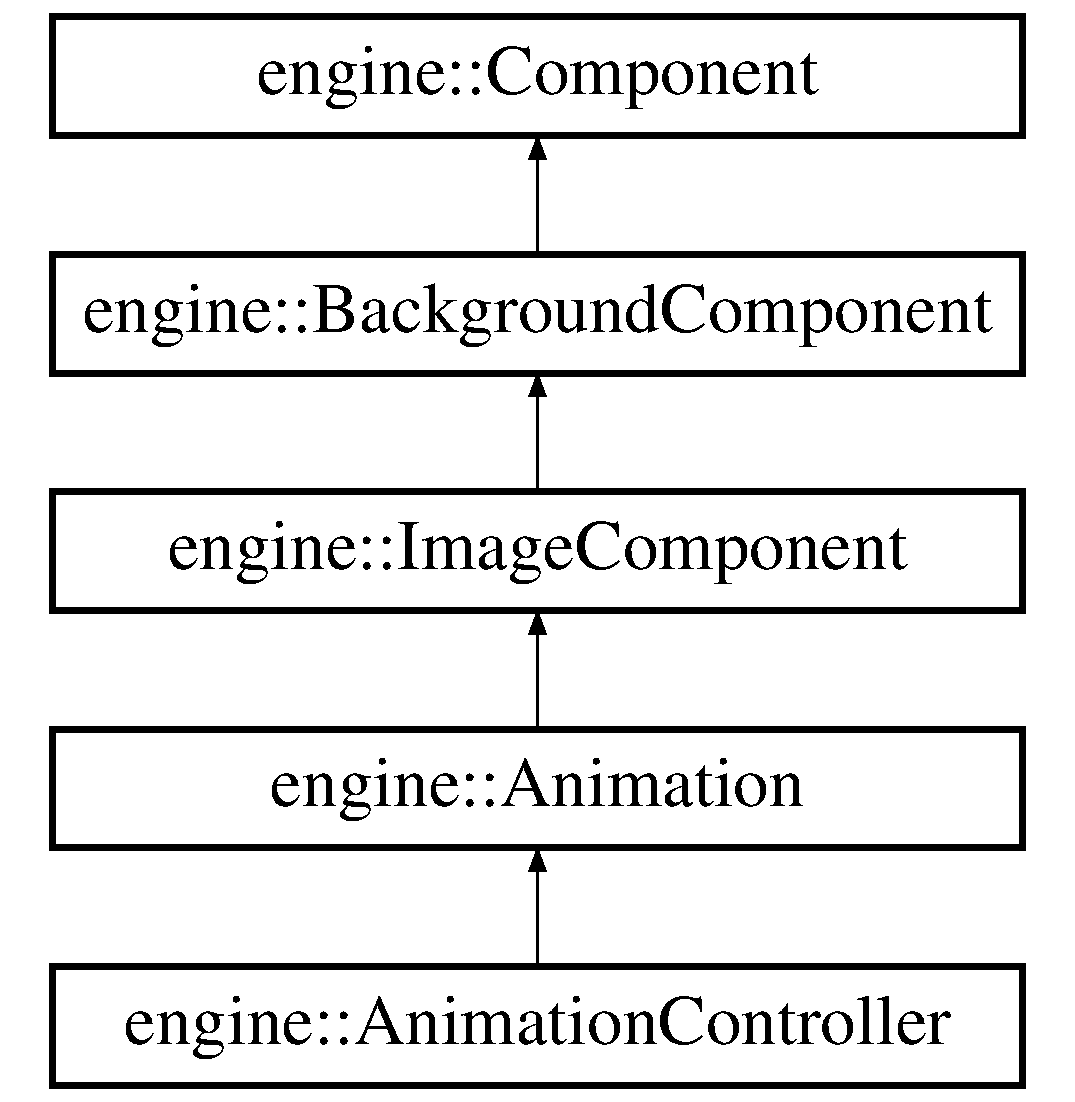
\includegraphics[height=5.000000cm]{classengine_1_1_animation}
\end{center}
\end{figure}
\subsection*{Public Member Functions}
\begin{DoxyCompactItemize}
\item 
\hyperlink{classengine_1_1_animation_a83f0a16cef7117f187ad596de38dd9d6}{Animation} ()
\item 
\hyperlink{classengine_1_1_animation_acc7e1092278297d6e029031115d147a6}{Animation} (\hyperlink{classengine_1_1_game_object}{Game\+Object} \&\hyperlink{classengine_1_1_component_ad4a4865ca4df98ebea34d04a4ec5ad07}{game\+Object}, std\+::string \hyperlink{classengine_1_1_background_component_aeffcb1aa8b67444e004413dee8c266b1}{image\+Path}, float animation\+Time, std\+::vector$<$ \hyperlink{classengine_1_1_sprite}{Sprite} $\ast$ $>$ sprite\+List, int start\+Frame, int end\+Frame, bool loop, double \hyperlink{classengine_1_1_image_component_aa27852286227a84dc9c9f01c9fe2add8}{zoom\+Factor})
\item 
\hyperlink{classengine_1_1_animation_a3bca75a5859165a3944d01efde626a2d}{Animation} (\hyperlink{classengine_1_1_game_object}{Game\+Object} \&\hyperlink{classengine_1_1_component_ad4a4865ca4df98ebea34d04a4ec5ad07}{game\+Object}, std\+::string \hyperlink{classengine_1_1_background_component_aeffcb1aa8b67444e004413dee8c266b1}{image\+Path}, float animation\+Time, std\+::vector$<$ \hyperlink{classengine_1_1_sprite}{Sprite} $\ast$ $>$ sprite\+List, int start\+Frame, int end\+Frame, bool loop, double \hyperlink{classengine_1_1_image_component_aa27852286227a84dc9c9f01c9fe2add8}{zoom\+Factor}, std\+::pair$<$ double, double $>$ position\+Relative\+To\+Object)
\item 
virtual \hyperlink{classengine_1_1_animation_a401b68793d4fbf48d481c030ee4b2a16}{$\sim$\+Animation} ()
\item 
void \hyperlink{classengine_1_1_animation_a219053e2c5bc9179fa355f14cf9bf032}{shutdown} ()
\begin{DoxyCompactList}\small\item\em inherits function that disable the game components \end{DoxyCompactList}\item 
void \hyperlink{classengine_1_1_animation_a5bc1f5aaee0372f573d4537dab43a162}{draw} ()
\begin{DoxyCompactList}\small\item\em inherits function that draw game objects. \end{DoxyCompactList}\item 
void \hyperlink{classengine_1_1_animation_aed6b685cec9e13063f171ce6bd49b9d7}{disable\+Component} ()
\begin{DoxyCompactList}\small\item\em disable components. \end{DoxyCompactList}\item 
std\+::string \hyperlink{classengine_1_1_animation_a6d7f93578e25311f51f2b3c737f885b2}{get\+Class\+Name} ()
\begin{DoxyCompactList}\small\item\em access the name of the class. \end{DoxyCompactList}\end{DoxyCompactItemize}
\subsection*{Public Attributes}
\begin{DoxyCompactItemize}
\item 
std\+::string \hyperlink{classengine_1_1_animation_a7db6aae9eef0e347e04af32b05a28476}{animation\+Name}
\item 
\hyperlink{namespaceengine_aa24807a1a7834d08efa99ae4672d3544}{Animation\+State} \hyperlink{classengine_1_1_animation_afa99aa470cb938b88ae337079d5628b7}{m\+State} = \hyperlink{namespaceengine_aa24807a1a7834d08efa99ae4672d3544a09d4d696b4e935115b9313e3c412509a}{Animation\+State\+::\+S\+T\+O\+P\+P\+ED}
\end{DoxyCompactItemize}
\subsection*{Additional Inherited Members}


\subsection{Detailed Description}


Definition at line 29 of file animation.\+hpp.



\subsection{Constructor \& Destructor Documentation}
\index{engine\+::\+Animation@{engine\+::\+Animation}!Animation@{Animation}}
\index{Animation@{Animation}!engine\+::\+Animation@{engine\+::\+Animation}}
\subsubsection[{\texorpdfstring{Animation()}{Animation()}}]{\setlength{\rightskip}{0pt plus 5cm}Animation\+::\+Animation (
\begin{DoxyParamCaption}
{}
\end{DoxyParamCaption}
)}\hypertarget{classengine_1_1_animation_a83f0a16cef7117f187ad596de38dd9d6}{}\label{classengine_1_1_animation_a83f0a16cef7117f187ad596de38dd9d6}


Definition at line 24 of file animation.\+cpp.

\index{engine\+::\+Animation@{engine\+::\+Animation}!Animation@{Animation}}
\index{Animation@{Animation}!engine\+::\+Animation@{engine\+::\+Animation}}
\subsubsection[{\texorpdfstring{Animation(\+Game\+Object \&game\+Object, std\+::string image\+Path, float animation\+Time, std\+::vector$<$ Sprite $\ast$ $>$ sprite\+List, int start\+Frame, int end\+Frame, bool loop, double zoom\+Factor)}{Animation(GameObject &gameObject, std::string imagePath, float animationTime, std::vector< Sprite * > spriteList, int startFrame, int endFrame, bool loop, double zoomFactor)}}]{\setlength{\rightskip}{0pt plus 5cm}Animation\+::\+Animation (
\begin{DoxyParamCaption}
\item[{{\bf Game\+Object} \&}]{game\+Object, }
\item[{std\+::string}]{image\+Path, }
\item[{float}]{animation\+Time, }
\item[{std\+::vector$<$ {\bf Sprite} $\ast$ $>$}]{sprite\+List, }
\item[{int}]{start\+Frame, }
\item[{int}]{end\+Frame, }
\item[{bool}]{loop, }
\item[{double}]{zoom\+Factor}
\end{DoxyParamCaption}
)}\hypertarget{classengine_1_1_animation_acc7e1092278297d6e029031115d147a6}{}\label{classengine_1_1_animation_acc7e1092278297d6e029031115d147a6}


Definition at line 26 of file animation.\+cpp.

\index{engine\+::\+Animation@{engine\+::\+Animation}!Animation@{Animation}}
\index{Animation@{Animation}!engine\+::\+Animation@{engine\+::\+Animation}}
\subsubsection[{\texorpdfstring{Animation(\+Game\+Object \&game\+Object, std\+::string image\+Path, float animation\+Time, std\+::vector$<$ Sprite $\ast$ $>$ sprite\+List, int start\+Frame, int end\+Frame, bool loop, double zoom\+Factor, std\+::pair$<$ double, double $>$ position\+Relative\+To\+Object)}{Animation(GameObject &gameObject, std::string imagePath, float animationTime, std::vector< Sprite * > spriteList, int startFrame, int endFrame, bool loop, double zoomFactor, std::pair< double, double > positionRelativeToObject)}}]{\setlength{\rightskip}{0pt plus 5cm}Animation\+::\+Animation (
\begin{DoxyParamCaption}
\item[{{\bf Game\+Object} \&}]{game\+Object, }
\item[{std\+::string}]{image\+Path, }
\item[{float}]{animation\+Time, }
\item[{std\+::vector$<$ {\bf Sprite} $\ast$ $>$}]{sprite\+List, }
\item[{int}]{start\+Frame, }
\item[{int}]{end\+Frame, }
\item[{bool}]{loop, }
\item[{double}]{zoom\+Factor, }
\item[{std\+::pair$<$ double, double $>$}]{position\+Relative\+To\+Object}
\end{DoxyParamCaption}
)}\hypertarget{classengine_1_1_animation_a3bca75a5859165a3944d01efde626a2d}{}\label{classengine_1_1_animation_a3bca75a5859165a3944d01efde626a2d}


Definition at line 46 of file animation.\+cpp.

\index{engine\+::\+Animation@{engine\+::\+Animation}!````~Animation@{$\sim$\+Animation}}
\index{````~Animation@{$\sim$\+Animation}!engine\+::\+Animation@{engine\+::\+Animation}}
\subsubsection[{\texorpdfstring{$\sim$\+Animation()}{~Animation()}}]{\setlength{\rightskip}{0pt plus 5cm}Animation\+::$\sim$\+Animation (
\begin{DoxyParamCaption}
{}
\end{DoxyParamCaption}
)\hspace{0.3cm}{\ttfamily [virtual]}}\hypertarget{classengine_1_1_animation_a401b68793d4fbf48d481c030ee4b2a16}{}\label{classengine_1_1_animation_a401b68793d4fbf48d481c030ee4b2a16}


Definition at line 68 of file animation.\+cpp.



\subsection{Member Function Documentation}
\index{engine\+::\+Animation@{engine\+::\+Animation}!disable\+Component@{disable\+Component}}
\index{disable\+Component@{disable\+Component}!engine\+::\+Animation@{engine\+::\+Animation}}
\subsubsection[{\texorpdfstring{disable\+Component()}{disableComponent()}}]{\setlength{\rightskip}{0pt plus 5cm}void Animation\+::disable\+Component (
\begin{DoxyParamCaption}
{}
\end{DoxyParamCaption}
)\hspace{0.3cm}{\ttfamily [virtual]}}\hypertarget{classengine_1_1_animation_aed6b685cec9e13063f171ce6bd49b9d7}{}\label{classengine_1_1_animation_aed6b685cec9e13063f171ce6bd49b9d7}


disable components. 

set the game object components state to disabled.

\begin{DoxyReturn}{Returns}
\char`\"{}void\char`\"{}. 
\end{DoxyReturn}


Reimplemented from \hyperlink{classengine_1_1_component_a9c42e55639174abeda044285a8b1db4b}{engine\+::\+Component}.



Definition at line 150 of file animation.\+cpp.

\index{engine\+::\+Animation@{engine\+::\+Animation}!draw@{draw}}
\index{draw@{draw}!engine\+::\+Animation@{engine\+::\+Animation}}
\subsubsection[{\texorpdfstring{draw()}{draw()}}]{\setlength{\rightskip}{0pt plus 5cm}void Animation\+::draw (
\begin{DoxyParamCaption}
{}
\end{DoxyParamCaption}
)\hspace{0.3cm}{\ttfamily [virtual]}}\hypertarget{classengine_1_1_animation_a5bc1f5aaee0372f573d4537dab43a162}{}\label{classengine_1_1_animation_a5bc1f5aaee0372f573d4537dab43a162}


inherits function that draw game objects. 

draws all the enabled game objects.

\begin{DoxyReturn}{Returns}
\char`\"{}void\char`\"{}. 
\end{DoxyReturn}


Reimplemented from \hyperlink{classengine_1_1_component_a3d20060d4af0bf0dd0c833994581bdfa}{engine\+::\+Component}.



Reimplemented in \hyperlink{classengine_1_1_animation_controller_a906d2adadfd5eeb2dc6edff3e2f15c45}{engine\+::\+Animation\+Controller}.



Definition at line 79 of file animation.\+cpp.

\index{engine\+::\+Animation@{engine\+::\+Animation}!get\+Class\+Name@{get\+Class\+Name}}
\index{get\+Class\+Name@{get\+Class\+Name}!engine\+::\+Animation@{engine\+::\+Animation}}
\subsubsection[{\texorpdfstring{get\+Class\+Name()}{getClassName()}}]{\setlength{\rightskip}{0pt plus 5cm}std\+::string engine\+::\+Animation\+::get\+Class\+Name (
\begin{DoxyParamCaption}
{}
\end{DoxyParamCaption}
)\hspace{0.3cm}{\ttfamily [inline]}, {\ttfamily [virtual]}}\hypertarget{classengine_1_1_animation_a6d7f93578e25311f51f2b3c737f885b2}{}\label{classengine_1_1_animation_a6d7f93578e25311f51f2b3c737f885b2}


access the name of the class. 

Used to get the private attribute class\+Name.

\begin{DoxyReturn}{Returns}
string that contains the scene name. 
\end{DoxyReturn}


Reimplemented from \hyperlink{classengine_1_1_component_a4341ed3c744b160590908bea151b6ca7}{engine\+::\+Component}.



Reimplemented in \hyperlink{classengine_1_1_animation_controller_a227866340161b386c3e39503a15e03cc}{engine\+::\+Animation\+Controller}.



Definition at line 62 of file animation.\+hpp.

\index{engine\+::\+Animation@{engine\+::\+Animation}!shutdown@{shutdown}}
\index{shutdown@{shutdown}!engine\+::\+Animation@{engine\+::\+Animation}}
\subsubsection[{\texorpdfstring{shutdown()}{shutdown()}}]{\setlength{\rightskip}{0pt plus 5cm}void Animation\+::shutdown (
\begin{DoxyParamCaption}
{}
\end{DoxyParamCaption}
)\hspace{0.3cm}{\ttfamily [virtual]}}\hypertarget{classengine_1_1_animation_a219053e2c5bc9179fa355f14cf9bf032}{}\label{classengine_1_1_animation_a219053e2c5bc9179fa355f14cf9bf032}


inherits function that disable the game components 

free the component pointers

\begin{DoxyReturn}{Returns}
\char`\"{}void\char`\"{}. 
\end{DoxyReturn}


Reimplemented from \hyperlink{classengine_1_1_component_a3e47775d51e78914bdfebba123354849}{engine\+::\+Component}.



Reimplemented in \hyperlink{classengine_1_1_animation_controller_a63ed3b30c0ea1fba109e6bed452c21ce}{engine\+::\+Animation\+Controller}.



Definition at line 70 of file animation.\+cpp.



\subsection{Member Data Documentation}
\index{engine\+::\+Animation@{engine\+::\+Animation}!animation\+Name@{animation\+Name}}
\index{animation\+Name@{animation\+Name}!engine\+::\+Animation@{engine\+::\+Animation}}
\subsubsection[{\texorpdfstring{animation\+Name}{animationName}}]{\setlength{\rightskip}{0pt plus 5cm}std\+::string engine\+::\+Animation\+::animation\+Name}\hypertarget{classengine_1_1_animation_a7db6aae9eef0e347e04af32b05a28476}{}\label{classengine_1_1_animation_a7db6aae9eef0e347e04af32b05a28476}


Definition at line 57 of file animation.\+hpp.

\index{engine\+::\+Animation@{engine\+::\+Animation}!m\+State@{m\+State}}
\index{m\+State@{m\+State}!engine\+::\+Animation@{engine\+::\+Animation}}
\subsubsection[{\texorpdfstring{m\+State}{mState}}]{\setlength{\rightskip}{0pt plus 5cm}{\bf Animation\+State} engine\+::\+Animation\+::m\+State = {\bf Animation\+State\+::\+S\+T\+O\+P\+P\+ED}}\hypertarget{classengine_1_1_animation_afa99aa470cb938b88ae337079d5628b7}{}\label{classengine_1_1_animation_afa99aa470cb938b88ae337079d5628b7}


Definition at line 58 of file animation.\+hpp.



The documentation for this class was generated from the following files\+:\begin{DoxyCompactItemize}
\item 
engine/include/\hyperlink{animation_8hpp}{animation.\+hpp}\item 
engine/src/\hyperlink{animation_8cpp}{animation.\+cpp}\end{DoxyCompactItemize}

\hypertarget{classengine_1_1_animation_controller}{}\section{engine\+:\+:Animation\+Controller Class Reference}
\label{classengine_1_1_animation_controller}\index{engine\+::\+Animation\+Controller@{engine\+::\+Animation\+Controller}}


{\ttfamily \#include $<$animation\+\_\+controller.\+hpp$>$}

Inheritance diagram for engine\+:\+:Animation\+Controller\+:\begin{figure}[H]
\begin{center}
\leavevmode
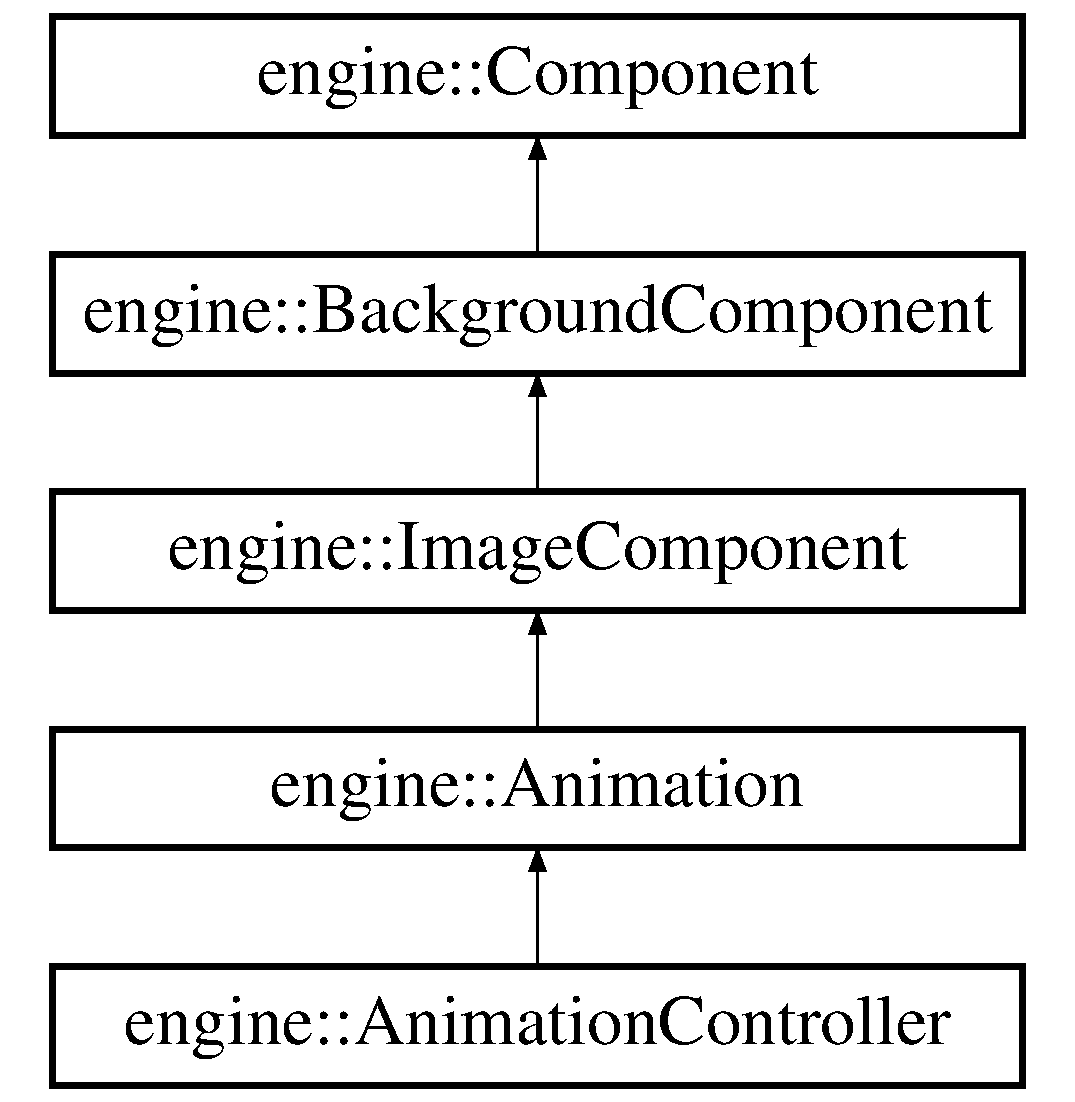
\includegraphics[height=5.000000cm]{classengine_1_1_animation_controller}
\end{center}
\end{figure}
\subsection*{Public Member Functions}
\begin{DoxyCompactItemize}
\item 
\hyperlink{classengine_1_1_animation_controller_a13976b0254122a71974b37ebc93b8526}{Animation\+Controller} ()
\item 
\hyperlink{classengine_1_1_animation_controller_ab56bec2905e143305453f2f2a88d0af8}{Animation\+Controller} (\hyperlink{classengine_1_1_game_object}{Game\+Object} \&\hyperlink{classengine_1_1_component_ad4a4865ca4df98ebea34d04a4ec5ad07}{game\+Object})
\item 
void \hyperlink{classengine_1_1_animation_controller_af52ba43bd14bb3cd912edd7a84afb3f9}{add\+Animation} (std\+::string \hyperlink{classengine_1_1_animation_a7db6aae9eef0e347e04af32b05a28476}{animation\+Name}, \hyperlink{classengine_1_1_animation}{Animation} \&animation)
\item 
void \hyperlink{classengine_1_1_animation_controller_af8950a96e4ac42fdab1d96bc79b951f4}{start\+Unique\+Animation} (std\+::string \hyperlink{classengine_1_1_animation_a7db6aae9eef0e347e04af32b05a28476}{animation\+Name})
\item 
void \hyperlink{classengine_1_1_animation_controller_ac0648702aa6724e46a4e377ae35221e1}{start\+Animation} (std\+::string \hyperlink{classengine_1_1_animation_a7db6aae9eef0e347e04af32b05a28476}{animation\+Name})
\item 
void \hyperlink{classengine_1_1_animation_controller_afc25ba59dc57193330399c491adff4bd}{stop\+Animation} (std\+::string \hyperlink{classengine_1_1_animation_a7db6aae9eef0e347e04af32b05a28476}{animation\+Name})
\item 
\hyperlink{namespaceengine_aa24807a1a7834d08efa99ae4672d3544}{Animation\+State} \hyperlink{classengine_1_1_animation_controller_a700251abe0a8f2145c84eb1d414f85c4}{get\+Animation\+Status} (std\+::string \hyperlink{classengine_1_1_animation_a7db6aae9eef0e347e04af32b05a28476}{animation\+Name})
\item 
void \hyperlink{classengine_1_1_animation_controller_ae40c2032604f044293d50c27da416f01}{init} ()
\begin{DoxyCompactList}\small\item\em inherits function that initialize the game components \end{DoxyCompactList}\item 
void \hyperlink{classengine_1_1_animation_controller_a63ed3b30c0ea1fba109e6bed452c21ce}{shutdown} ()
\begin{DoxyCompactList}\small\item\em inherits function that disable the game components \end{DoxyCompactList}\item 
void \hyperlink{classengine_1_1_animation_controller_a906d2adadfd5eeb2dc6edff3e2f15c45}{draw} ()
\begin{DoxyCompactList}\small\item\em inherits function that draw game objects. \end{DoxyCompactList}\item 
void \hyperlink{classengine_1_1_animation_controller_a90f9286c95905815716f87bf6aae733c}{next\+Sprite} (std\+::string name)
\item 
std\+::string \hyperlink{classengine_1_1_animation_controller_a227866340161b386c3e39503a15e03cc}{get\+Class\+Name} ()
\begin{DoxyCompactList}\small\item\em access the name of the class. \end{DoxyCompactList}\end{DoxyCompactItemize}
\subsection*{Additional Inherited Members}


\subsection{Detailed Description}


Definition at line 23 of file animation\+\_\+controller.\+hpp.



\subsection{Constructor \& Destructor Documentation}
\index{engine\+::\+Animation\+Controller@{engine\+::\+Animation\+Controller}!Animation\+Controller@{Animation\+Controller}}
\index{Animation\+Controller@{Animation\+Controller}!engine\+::\+Animation\+Controller@{engine\+::\+Animation\+Controller}}
\subsubsection[{\texorpdfstring{Animation\+Controller()}{AnimationController()}}]{\setlength{\rightskip}{0pt plus 5cm}Animation\+Controller\+::\+Animation\+Controller (
\begin{DoxyParamCaption}
{}
\end{DoxyParamCaption}
)}\hypertarget{classengine_1_1_animation_controller_a13976b0254122a71974b37ebc93b8526}{}\label{classengine_1_1_animation_controller_a13976b0254122a71974b37ebc93b8526}


Definition at line 40 of file animation\+\_\+controller.\+cpp.

\index{engine\+::\+Animation\+Controller@{engine\+::\+Animation\+Controller}!Animation\+Controller@{Animation\+Controller}}
\index{Animation\+Controller@{Animation\+Controller}!engine\+::\+Animation\+Controller@{engine\+::\+Animation\+Controller}}
\subsubsection[{\texorpdfstring{Animation\+Controller(\+Game\+Object \&game\+Object)}{AnimationController(GameObject &gameObject)}}]{\setlength{\rightskip}{0pt plus 5cm}Animation\+Controller\+::\+Animation\+Controller (
\begin{DoxyParamCaption}
\item[{{\bf Game\+Object} \&}]{game\+Object}
\end{DoxyParamCaption}
)}\hypertarget{classengine_1_1_animation_controller_ab56bec2905e143305453f2f2a88d0af8}{}\label{classengine_1_1_animation_controller_ab56bec2905e143305453f2f2a88d0af8}


Definition at line 44 of file animation\+\_\+controller.\+cpp.



\subsection{Member Function Documentation}
\index{engine\+::\+Animation\+Controller@{engine\+::\+Animation\+Controller}!add\+Animation@{add\+Animation}}
\index{add\+Animation@{add\+Animation}!engine\+::\+Animation\+Controller@{engine\+::\+Animation\+Controller}}
\subsubsection[{\texorpdfstring{add\+Animation(std\+::string animation\+Name, Animation \&animation)}{addAnimation(std::string animationName, Animation &animation)}}]{\setlength{\rightskip}{0pt plus 5cm}void Animation\+Controller\+::add\+Animation (
\begin{DoxyParamCaption}
\item[{std\+::string}]{animation\+Name, }
\item[{{\bf Animation} \&}]{animation}
\end{DoxyParamCaption}
)}\hypertarget{classengine_1_1_animation_controller_af52ba43bd14bb3cd912edd7a84afb3f9}{}\label{classengine_1_1_animation_controller_af52ba43bd14bb3cd912edd7a84afb3f9}


Definition at line 49 of file animation\+\_\+controller.\+cpp.

\index{engine\+::\+Animation\+Controller@{engine\+::\+Animation\+Controller}!draw@{draw}}
\index{draw@{draw}!engine\+::\+Animation\+Controller@{engine\+::\+Animation\+Controller}}
\subsubsection[{\texorpdfstring{draw()}{draw()}}]{\setlength{\rightskip}{0pt plus 5cm}void Animation\+Controller\+::draw (
\begin{DoxyParamCaption}
{}
\end{DoxyParamCaption}
)\hspace{0.3cm}{\ttfamily [virtual]}}\hypertarget{classengine_1_1_animation_controller_a906d2adadfd5eeb2dc6edff3e2f15c45}{}\label{classengine_1_1_animation_controller_a906d2adadfd5eeb2dc6edff3e2f15c45}


inherits function that draw game objects. 

draws all the enabled game objects.

\begin{DoxyReturn}{Returns}
\char`\"{}void\char`\"{}. 
\end{DoxyReturn}


Reimplemented from \hyperlink{classengine_1_1_animation_a5bc1f5aaee0372f573d4537dab43a162}{engine\+::\+Animation}.



Definition at line 24 of file animation\+\_\+controller.\+cpp.

\index{engine\+::\+Animation\+Controller@{engine\+::\+Animation\+Controller}!get\+Animation\+Status@{get\+Animation\+Status}}
\index{get\+Animation\+Status@{get\+Animation\+Status}!engine\+::\+Animation\+Controller@{engine\+::\+Animation\+Controller}}
\subsubsection[{\texorpdfstring{get\+Animation\+Status(std\+::string animation\+Name)}{getAnimationStatus(std::string animationName)}}]{\setlength{\rightskip}{0pt plus 5cm}{\bf Animation\+State} Animation\+Controller\+::get\+Animation\+Status (
\begin{DoxyParamCaption}
\item[{std\+::string}]{animation\+Name}
\end{DoxyParamCaption}
)}\hypertarget{classengine_1_1_animation_controller_a700251abe0a8f2145c84eb1d414f85c4}{}\label{classengine_1_1_animation_controller_a700251abe0a8f2145c84eb1d414f85c4}


Definition at line 98 of file animation\+\_\+controller.\+cpp.

\index{engine\+::\+Animation\+Controller@{engine\+::\+Animation\+Controller}!get\+Class\+Name@{get\+Class\+Name}}
\index{get\+Class\+Name@{get\+Class\+Name}!engine\+::\+Animation\+Controller@{engine\+::\+Animation\+Controller}}
\subsubsection[{\texorpdfstring{get\+Class\+Name()}{getClassName()}}]{\setlength{\rightskip}{0pt plus 5cm}std\+::string engine\+::\+Animation\+Controller\+::get\+Class\+Name (
\begin{DoxyParamCaption}
{}
\end{DoxyParamCaption}
)\hspace{0.3cm}{\ttfamily [inline]}, {\ttfamily [virtual]}}\hypertarget{classengine_1_1_animation_controller_a227866340161b386c3e39503a15e03cc}{}\label{classengine_1_1_animation_controller_a227866340161b386c3e39503a15e03cc}


access the name of the class. 

Used to get the private attribute class\+Name.

\begin{DoxyReturn}{Returns}
string that contains the scene name. 
\end{DoxyReturn}


Reimplemented from \hyperlink{classengine_1_1_animation_a6d7f93578e25311f51f2b3c737f885b2}{engine\+::\+Animation}.



Definition at line 45 of file animation\+\_\+controller.\+hpp.

\index{engine\+::\+Animation\+Controller@{engine\+::\+Animation\+Controller}!init@{init}}
\index{init@{init}!engine\+::\+Animation\+Controller@{engine\+::\+Animation\+Controller}}
\subsubsection[{\texorpdfstring{init()}{init()}}]{\setlength{\rightskip}{0pt plus 5cm}void Animation\+Controller\+::init (
\begin{DoxyParamCaption}
{}
\end{DoxyParamCaption}
)\hspace{0.3cm}{\ttfamily [virtual]}}\hypertarget{classengine_1_1_animation_controller_ae40c2032604f044293d50c27da416f01}{}\label{classengine_1_1_animation_controller_ae40c2032604f044293d50c27da416f01}


inherits function that initialize the game components 

Set all game components to enable

\begin{DoxyReturn}{Returns}
\char`\"{}void\char`\"{}. 
\end{DoxyReturn}


Reimplemented from \hyperlink{classengine_1_1_component_aa0bf4fb5f4bc0de25d3f7beef3a3ca45}{engine\+::\+Component}.



Definition at line 17 of file animation\+\_\+controller.\+cpp.

\index{engine\+::\+Animation\+Controller@{engine\+::\+Animation\+Controller}!next\+Sprite@{next\+Sprite}}
\index{next\+Sprite@{next\+Sprite}!engine\+::\+Animation\+Controller@{engine\+::\+Animation\+Controller}}
\subsubsection[{\texorpdfstring{next\+Sprite(std\+::string name)}{nextSprite(std::string name)}}]{\setlength{\rightskip}{0pt plus 5cm}void engine\+::\+Animation\+Controller\+::next\+Sprite (
\begin{DoxyParamCaption}
\item[{std\+::string}]{name}
\end{DoxyParamCaption}
)}\hypertarget{classengine_1_1_animation_controller_a90f9286c95905815716f87bf6aae733c}{}\label{classengine_1_1_animation_controller_a90f9286c95905815716f87bf6aae733c}
\index{engine\+::\+Animation\+Controller@{engine\+::\+Animation\+Controller}!shutdown@{shutdown}}
\index{shutdown@{shutdown}!engine\+::\+Animation\+Controller@{engine\+::\+Animation\+Controller}}
\subsubsection[{\texorpdfstring{shutdown()}{shutdown()}}]{\setlength{\rightskip}{0pt plus 5cm}void Animation\+Controller\+::shutdown (
\begin{DoxyParamCaption}
{}
\end{DoxyParamCaption}
)\hspace{0.3cm}{\ttfamily [virtual]}}\hypertarget{classengine_1_1_animation_controller_a63ed3b30c0ea1fba109e6bed452c21ce}{}\label{classengine_1_1_animation_controller_a63ed3b30c0ea1fba109e6bed452c21ce}


inherits function that disable the game components 

free the component pointers

\begin{DoxyReturn}{Returns}
\char`\"{}void\char`\"{}. 
\end{DoxyReturn}


Reimplemented from \hyperlink{classengine_1_1_animation_a219053e2c5bc9179fa355f14cf9bf032}{engine\+::\+Animation}.



Definition at line 33 of file animation\+\_\+controller.\+cpp.

\index{engine\+::\+Animation\+Controller@{engine\+::\+Animation\+Controller}!start\+Animation@{start\+Animation}}
\index{start\+Animation@{start\+Animation}!engine\+::\+Animation\+Controller@{engine\+::\+Animation\+Controller}}
\subsubsection[{\texorpdfstring{start\+Animation(std\+::string animation\+Name)}{startAnimation(std::string animationName)}}]{\setlength{\rightskip}{0pt plus 5cm}void Animation\+Controller\+::start\+Animation (
\begin{DoxyParamCaption}
\item[{std\+::string}]{animation\+Name}
\end{DoxyParamCaption}
)}\hypertarget{classengine_1_1_animation_controller_ac0648702aa6724e46a4e377ae35221e1}{}\label{classengine_1_1_animation_controller_ac0648702aa6724e46a4e377ae35221e1}


Definition at line 74 of file animation\+\_\+controller.\+cpp.

\index{engine\+::\+Animation\+Controller@{engine\+::\+Animation\+Controller}!start\+Unique\+Animation@{start\+Unique\+Animation}}
\index{start\+Unique\+Animation@{start\+Unique\+Animation}!engine\+::\+Animation\+Controller@{engine\+::\+Animation\+Controller}}
\subsubsection[{\texorpdfstring{start\+Unique\+Animation(std\+::string animation\+Name)}{startUniqueAnimation(std::string animationName)}}]{\setlength{\rightskip}{0pt plus 5cm}void Animation\+Controller\+::start\+Unique\+Animation (
\begin{DoxyParamCaption}
\item[{std\+::string}]{animation\+Name}
\end{DoxyParamCaption}
)}\hypertarget{classengine_1_1_animation_controller_af8950a96e4ac42fdab1d96bc79b951f4}{}\label{classengine_1_1_animation_controller_af8950a96e4ac42fdab1d96bc79b951f4}


Definition at line 55 of file animation\+\_\+controller.\+cpp.

\index{engine\+::\+Animation\+Controller@{engine\+::\+Animation\+Controller}!stop\+Animation@{stop\+Animation}}
\index{stop\+Animation@{stop\+Animation}!engine\+::\+Animation\+Controller@{engine\+::\+Animation\+Controller}}
\subsubsection[{\texorpdfstring{stop\+Animation(std\+::string animation\+Name)}{stopAnimation(std::string animationName)}}]{\setlength{\rightskip}{0pt plus 5cm}void Animation\+Controller\+::stop\+Animation (
\begin{DoxyParamCaption}
\item[{std\+::string}]{animation\+Name}
\end{DoxyParamCaption}
)}\hypertarget{classengine_1_1_animation_controller_afc25ba59dc57193330399c491adff4bd}{}\label{classengine_1_1_animation_controller_afc25ba59dc57193330399c491adff4bd}


Definition at line 88 of file animation\+\_\+controller.\+cpp.



The documentation for this class was generated from the following files\+:\begin{DoxyCompactItemize}
\item 
engine/include/\hyperlink{animation__controller_8hpp}{animation\+\_\+controller.\+hpp}\item 
engine/src/\hyperlink{animation__controller_8cpp}{animation\+\_\+controller.\+cpp}\end{DoxyCompactItemize}

\hypertarget{classengine_1_1_assets_manager}{}\section{engine\+:\+:Assets\+Manager Class Reference}
\label{classengine_1_1_assets_manager}\index{engine\+::\+Assets\+Manager@{engine\+::\+Assets\+Manager}}


\hyperlink{classengine_1_1_assets_manager}{Assets\+Manager} class.  




{\ttfamily \#include $<$assets\+\_\+manager.\+hpp$>$}

\subsection*{Public Member Functions}
\begin{DoxyCompactItemize}
\item 
\hyperlink{classengine_1_1_assets_manager_a04b603ba0f5398921d0a2d13c8535acf}{Assets\+Manager} ()
\begin{DoxyCompactList}\small\item\em Default constructor for the assets manager. \end{DoxyCompactList}\item 
\hyperlink{structengine_1_1_image}{Image} $\ast$ \hyperlink{classengine_1_1_assets_manager_a3ba125182551280bcfdaf50aed863950}{Load\+Image} (std\+::string image\+Path)
\item 
Mix\+\_\+\+Music $\ast$ \hyperlink{classengine_1_1_assets_manager_a7244ff799dc6f501c09ef13686b7a991}{Load\+Music} (std\+::string audio\+Path)
\item 
Mix\+\_\+\+Chunk $\ast$ \hyperlink{classengine_1_1_assets_manager_a7592447ab48c251bab45c3a1540828fe}{Load\+Sound} (std\+::string audio\+Path)
\end{DoxyCompactItemize}


\subsection{Detailed Description}
\hyperlink{classengine_1_1_assets_manager}{Assets\+Manager} class. 

This class is responsible for assets the \hyperlink{structengine_1_1_image}{Image} map, music map and sound map. 

Definition at line 34 of file assets\+\_\+manager.\+hpp.



\subsection{Constructor \& Destructor Documentation}
\index{engine\+::\+Assets\+Manager@{engine\+::\+Assets\+Manager}!Assets\+Manager@{Assets\+Manager}}
\index{Assets\+Manager@{Assets\+Manager}!engine\+::\+Assets\+Manager@{engine\+::\+Assets\+Manager}}
\subsubsection[{\texorpdfstring{Assets\+Manager()}{AssetsManager()}}]{\setlength{\rightskip}{0pt plus 5cm}Assets\+Manager\+::\+Assets\+Manager (
\begin{DoxyParamCaption}
{}
\end{DoxyParamCaption}
)}\hypertarget{classengine_1_1_assets_manager_a04b603ba0f5398921d0a2d13c8535acf}{}\label{classengine_1_1_assets_manager_a04b603ba0f5398921d0a2d13c8535acf}


Default constructor for the assets manager. 

\begin{DoxyReturn}{Returns}
\char`\"{}void\char`\"{}. 
\end{DoxyReturn}


Definition at line 20 of file assets\+\_\+manager.\+cpp.



\subsection{Member Function Documentation}
\index{engine\+::\+Assets\+Manager@{engine\+::\+Assets\+Manager}!Load\+Image@{Load\+Image}}
\index{Load\+Image@{Load\+Image}!engine\+::\+Assets\+Manager@{engine\+::\+Assets\+Manager}}
\subsubsection[{\texorpdfstring{Load\+Image(std\+::string image\+Path)}{LoadImage(std::string imagePath)}}]{\setlength{\rightskip}{0pt plus 5cm}{\bf Image} $\ast$ Assets\+Manager\+::\+Load\+Image (
\begin{DoxyParamCaption}
\item[{std\+::string}]{image\+Path}
\end{DoxyParamCaption}
)}\hypertarget{classengine_1_1_assets_manager_a3ba125182551280bcfdaf50aed863950}{}\label{classengine_1_1_assets_manager_a3ba125182551280bcfdaf50aed863950}


Definition at line 24 of file assets\+\_\+manager.\+cpp.

\index{engine\+::\+Assets\+Manager@{engine\+::\+Assets\+Manager}!Load\+Music@{Load\+Music}}
\index{Load\+Music@{Load\+Music}!engine\+::\+Assets\+Manager@{engine\+::\+Assets\+Manager}}
\subsubsection[{\texorpdfstring{Load\+Music(std\+::string audio\+Path)}{LoadMusic(std::string audioPath)}}]{\setlength{\rightskip}{0pt plus 5cm}Mix\+\_\+\+Music $\ast$ Assets\+Manager\+::\+Load\+Music (
\begin{DoxyParamCaption}
\item[{std\+::string}]{audio\+Path}
\end{DoxyParamCaption}
)}\hypertarget{classengine_1_1_assets_manager_a7244ff799dc6f501c09ef13686b7a991}{}\label{classengine_1_1_assets_manager_a7244ff799dc6f501c09ef13686b7a991}


Definition at line 86 of file assets\+\_\+manager.\+cpp.

\index{engine\+::\+Assets\+Manager@{engine\+::\+Assets\+Manager}!Load\+Sound@{Load\+Sound}}
\index{Load\+Sound@{Load\+Sound}!engine\+::\+Assets\+Manager@{engine\+::\+Assets\+Manager}}
\subsubsection[{\texorpdfstring{Load\+Sound(std\+::string audio\+Path)}{LoadSound(std::string audioPath)}}]{\setlength{\rightskip}{0pt plus 5cm}Mix\+\_\+\+Chunk $\ast$ Assets\+Manager\+::\+Load\+Sound (
\begin{DoxyParamCaption}
\item[{std\+::string}]{audio\+Path}
\end{DoxyParamCaption}
)}\hypertarget{classengine_1_1_assets_manager_a7592447ab48c251bab45c3a1540828fe}{}\label{classengine_1_1_assets_manager_a7592447ab48c251bab45c3a1540828fe}


Definition at line 129 of file assets\+\_\+manager.\+cpp.



The documentation for this class was generated from the following files\+:\begin{DoxyCompactItemize}
\item 
engine/include/\hyperlink{assets__manager_8hpp}{assets\+\_\+manager.\+hpp}\item 
engine/src/\hyperlink{assets__manager_8cpp}{assets\+\_\+manager.\+cpp}\end{DoxyCompactItemize}

\hypertarget{classengine_1_1_audio_component}{}\section{engine\+:\+:Audio\+Component Class Reference}
\label{classengine_1_1_audio_component}\index{engine\+::\+Audio\+Component@{engine\+::\+Audio\+Component}}


{\ttfamily \#include $<$audio\+\_\+component.\+hpp$>$}

Inheritance diagram for engine\+:\+:Audio\+Component\+:\begin{figure}[H]
\begin{center}
\leavevmode
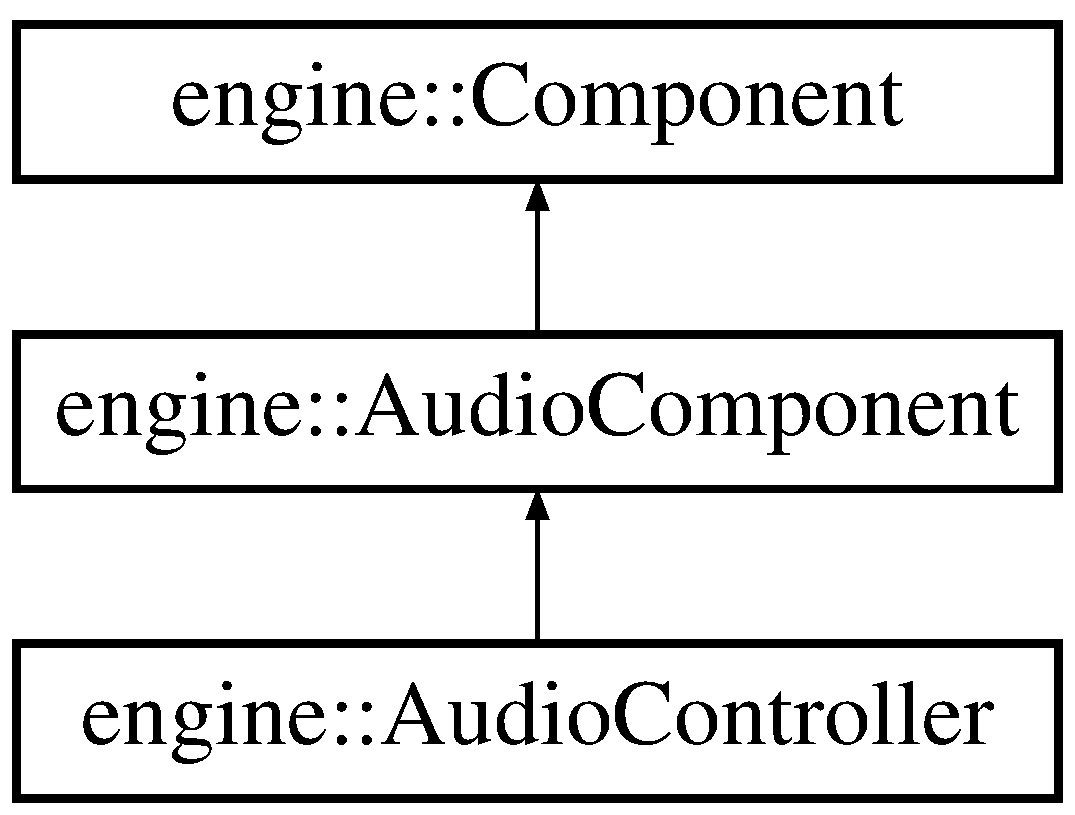
\includegraphics[height=3.000000cm]{classengine_1_1_audio_component}
\end{center}
\end{figure}
\subsection*{Public Member Functions}
\begin{DoxyCompactItemize}
\item 
\hyperlink{classengine_1_1_audio_component_aaea64af7cd81778f6737f0a4bee35394}{Audio\+Component} ()
\item 
virtual \hyperlink{classengine_1_1_audio_component_a68bf2351458d61601aad7abeb3f58588}{$\sim$\+Audio\+Component} ()
\item 
\hyperlink{classengine_1_1_audio_component_a59af70319c3b0c81a66b5c1b9525cb46}{Audio\+Component} (\hyperlink{classengine_1_1_game_object}{Game\+Object} \&\hyperlink{classengine_1_1_component_ad4a4865ca4df98ebea34d04a4ec5ad07}{game\+Object}, std\+::string audio\+Path, bool is\+Music, bool play\+On\+Start)
\item 
void \hyperlink{classengine_1_1_audio_component_a61f7e9f09253a0619ed979276267150c}{init} ()
\begin{DoxyCompactList}\small\item\em inherits function that initialize the game components \end{DoxyCompactList}\item 
void \hyperlink{classengine_1_1_audio_component_acb42c8fa38793ff0fe6c0652bbb9eac9}{shutdown} ()
\begin{DoxyCompactList}\small\item\em inherits function that disable the game components \end{DoxyCompactList}\item 
void \hyperlink{classengine_1_1_audio_component_aa35e7f57c104c2281680bb13764e4ef0}{update\+Code} ()
\begin{DoxyCompactList}\small\item\em inherits function that update the game code. \end{DoxyCompactList}\item 
void \hyperlink{classengine_1_1_audio_component_a09cc2c39a6bb97c79257a4593ab57e42}{play} (int loops, int channel)
\item 
void \hyperlink{classengine_1_1_audio_component_aa7274401541925ff8b8a639de01b2b7e}{stop} (int channel)
\item 
void \hyperlink{classengine_1_1_audio_component_adbc0fe9c86ccabf06cc685882e98701f}{pause} (int channel)
\item 
bool \hyperlink{classengine_1_1_audio_component_a3aeb1bb7591da6da496461a8384cff9c}{get\+Is\+Music} ()
\end{DoxyCompactItemize}
\subsection*{Public Attributes}
\begin{DoxyCompactItemize}
\item 
\hyperlink{namespaceengine_a5de9278ae356d4ff4fe8864ebf683bc8}{Audio\+State} \hyperlink{classengine_1_1_audio_component_a78e6ef6497d0f325df7aab194a1ab449}{audio\+State}
\end{DoxyCompactItemize}
\subsection*{Additional Inherited Members}


\subsection{Detailed Description}


Definition at line 39 of file audio\+\_\+component.\+hpp.



\subsection{Constructor \& Destructor Documentation}
\index{engine\+::\+Audio\+Component@{engine\+::\+Audio\+Component}!Audio\+Component@{Audio\+Component}}
\index{Audio\+Component@{Audio\+Component}!engine\+::\+Audio\+Component@{engine\+::\+Audio\+Component}}
\subsubsection[{\texorpdfstring{Audio\+Component()}{AudioComponent()}}]{\setlength{\rightskip}{0pt plus 5cm}Audio\+Component\+::\+Audio\+Component (
\begin{DoxyParamCaption}
{}
\end{DoxyParamCaption}
)}\hypertarget{classengine_1_1_audio_component_aaea64af7cd81778f6737f0a4bee35394}{}\label{classengine_1_1_audio_component_aaea64af7cd81778f6737f0a4bee35394}


Definition at line 21 of file audio\+\_\+component.\+cpp.

\index{engine\+::\+Audio\+Component@{engine\+::\+Audio\+Component}!````~Audio\+Component@{$\sim$\+Audio\+Component}}
\index{````~Audio\+Component@{$\sim$\+Audio\+Component}!engine\+::\+Audio\+Component@{engine\+::\+Audio\+Component}}
\subsubsection[{\texorpdfstring{$\sim$\+Audio\+Component()}{~AudioComponent()}}]{\setlength{\rightskip}{0pt plus 5cm}Audio\+Component\+::$\sim$\+Audio\+Component (
\begin{DoxyParamCaption}
{}
\end{DoxyParamCaption}
)\hspace{0.3cm}{\ttfamily [virtual]}}\hypertarget{classengine_1_1_audio_component_a68bf2351458d61601aad7abeb3f58588}{}\label{classengine_1_1_audio_component_a68bf2351458d61601aad7abeb3f58588}


Definition at line 24 of file audio\+\_\+component.\+cpp.

\index{engine\+::\+Audio\+Component@{engine\+::\+Audio\+Component}!Audio\+Component@{Audio\+Component}}
\index{Audio\+Component@{Audio\+Component}!engine\+::\+Audio\+Component@{engine\+::\+Audio\+Component}}
\subsubsection[{\texorpdfstring{Audio\+Component(\+Game\+Object \&game\+Object, std\+::string audio\+Path, bool is\+Music, bool play\+On\+Start)}{AudioComponent(GameObject &gameObject, std::string audioPath, bool isMusic, bool playOnStart)}}]{\setlength{\rightskip}{0pt plus 5cm}Audio\+Component\+::\+Audio\+Component (
\begin{DoxyParamCaption}
\item[{{\bf Game\+Object} \&}]{game\+Object, }
\item[{std\+::string}]{audio\+Path, }
\item[{bool}]{is\+Music, }
\item[{bool}]{play\+On\+Start}
\end{DoxyParamCaption}
)}\hypertarget{classengine_1_1_audio_component_a59af70319c3b0c81a66b5c1b9525cb46}{}\label{classengine_1_1_audio_component_a59af70319c3b0c81a66b5c1b9525cb46}


Definition at line 32 of file audio\+\_\+component.\+cpp.



\subsection{Member Function Documentation}
\index{engine\+::\+Audio\+Component@{engine\+::\+Audio\+Component}!get\+Is\+Music@{get\+Is\+Music}}
\index{get\+Is\+Music@{get\+Is\+Music}!engine\+::\+Audio\+Component@{engine\+::\+Audio\+Component}}
\subsubsection[{\texorpdfstring{get\+Is\+Music()}{getIsMusic()}}]{\setlength{\rightskip}{0pt plus 5cm}bool engine\+::\+Audio\+Component\+::get\+Is\+Music (
\begin{DoxyParamCaption}
{}
\end{DoxyParamCaption}
)\hspace{0.3cm}{\ttfamily [inline]}}\hypertarget{classengine_1_1_audio_component_a3aeb1bb7591da6da496461a8384cff9c}{}\label{classengine_1_1_audio_component_a3aeb1bb7591da6da496461a8384cff9c}


Definition at line 62 of file audio\+\_\+component.\+hpp.

\index{engine\+::\+Audio\+Component@{engine\+::\+Audio\+Component}!init@{init}}
\index{init@{init}!engine\+::\+Audio\+Component@{engine\+::\+Audio\+Component}}
\subsubsection[{\texorpdfstring{init()}{init()}}]{\setlength{\rightskip}{0pt plus 5cm}void Audio\+Component\+::init (
\begin{DoxyParamCaption}
{}
\end{DoxyParamCaption}
)\hspace{0.3cm}{\ttfamily [virtual]}}\hypertarget{classengine_1_1_audio_component_a61f7e9f09253a0619ed979276267150c}{}\label{classengine_1_1_audio_component_a61f7e9f09253a0619ed979276267150c}


inherits function that initialize the game components 

Set all game components to enable

\begin{DoxyReturn}{Returns}
\char`\"{}void\char`\"{}. 
\end{DoxyReturn}


Reimplemented from \hyperlink{classengine_1_1_component_aa0bf4fb5f4bc0de25d3f7beef3a3ca45}{engine\+::\+Component}.



Reimplemented in \hyperlink{classengine_1_1_audio_controller_a34af3c91cadbf4a97eafdd3e311671c9}{engine\+::\+Audio\+Controller}.



Definition at line 50 of file audio\+\_\+component.\+cpp.

\index{engine\+::\+Audio\+Component@{engine\+::\+Audio\+Component}!pause@{pause}}
\index{pause@{pause}!engine\+::\+Audio\+Component@{engine\+::\+Audio\+Component}}
\subsubsection[{\texorpdfstring{pause(int channel)}{pause(int channel)}}]{\setlength{\rightskip}{0pt plus 5cm}void Audio\+Component\+::pause (
\begin{DoxyParamCaption}
\item[{int}]{channel}
\end{DoxyParamCaption}
)}\hypertarget{classengine_1_1_audio_component_adbc0fe9c86ccabf06cc685882e98701f}{}\label{classengine_1_1_audio_component_adbc0fe9c86ccabf06cc685882e98701f}


Definition at line 150 of file audio\+\_\+component.\+cpp.

\index{engine\+::\+Audio\+Component@{engine\+::\+Audio\+Component}!play@{play}}
\index{play@{play}!engine\+::\+Audio\+Component@{engine\+::\+Audio\+Component}}
\subsubsection[{\texorpdfstring{play(int loops, int channel)}{play(int loops, int channel)}}]{\setlength{\rightskip}{0pt plus 5cm}void Audio\+Component\+::play (
\begin{DoxyParamCaption}
\item[{int}]{loops, }
\item[{int}]{channel}
\end{DoxyParamCaption}
)}\hypertarget{classengine_1_1_audio_component_a09cc2c39a6bb97c79257a4593ab57e42}{}\label{classengine_1_1_audio_component_a09cc2c39a6bb97c79257a4593ab57e42}


Definition at line 100 of file audio\+\_\+component.\+cpp.

\index{engine\+::\+Audio\+Component@{engine\+::\+Audio\+Component}!shutdown@{shutdown}}
\index{shutdown@{shutdown}!engine\+::\+Audio\+Component@{engine\+::\+Audio\+Component}}
\subsubsection[{\texorpdfstring{shutdown()}{shutdown()}}]{\setlength{\rightskip}{0pt plus 5cm}void Audio\+Component\+::shutdown (
\begin{DoxyParamCaption}
{}
\end{DoxyParamCaption}
)\hspace{0.3cm}{\ttfamily [virtual]}}\hypertarget{classengine_1_1_audio_component_acb42c8fa38793ff0fe6c0652bbb9eac9}{}\label{classengine_1_1_audio_component_acb42c8fa38793ff0fe6c0652bbb9eac9}


inherits function that disable the game components 

free the component pointers

\begin{DoxyReturn}{Returns}
\char`\"{}void\char`\"{}. 
\end{DoxyReturn}


Reimplemented from \hyperlink{classengine_1_1_component_a3e47775d51e78914bdfebba123354849}{engine\+::\+Component}.



Reimplemented in \hyperlink{classengine_1_1_audio_controller_aaeb8eaadaa523db5e3608f019fe1bf8e}{engine\+::\+Audio\+Controller}.



Definition at line 81 of file audio\+\_\+component.\+cpp.

\index{engine\+::\+Audio\+Component@{engine\+::\+Audio\+Component}!stop@{stop}}
\index{stop@{stop}!engine\+::\+Audio\+Component@{engine\+::\+Audio\+Component}}
\subsubsection[{\texorpdfstring{stop(int channel)}{stop(int channel)}}]{\setlength{\rightskip}{0pt plus 5cm}void Audio\+Component\+::stop (
\begin{DoxyParamCaption}
\item[{int}]{channel}
\end{DoxyParamCaption}
)}\hypertarget{classengine_1_1_audio_component_aa7274401541925ff8b8a639de01b2b7e}{}\label{classengine_1_1_audio_component_aa7274401541925ff8b8a639de01b2b7e}


Definition at line 131 of file audio\+\_\+component.\+cpp.

\index{engine\+::\+Audio\+Component@{engine\+::\+Audio\+Component}!update\+Code@{update\+Code}}
\index{update\+Code@{update\+Code}!engine\+::\+Audio\+Component@{engine\+::\+Audio\+Component}}
\subsubsection[{\texorpdfstring{update\+Code()}{updateCode()}}]{\setlength{\rightskip}{0pt plus 5cm}void Audio\+Component\+::update\+Code (
\begin{DoxyParamCaption}
{}
\end{DoxyParamCaption}
)\hspace{0.3cm}{\ttfamily [virtual]}}\hypertarget{classengine_1_1_audio_component_aa35e7f57c104c2281680bb13764e4ef0}{}\label{classengine_1_1_audio_component_aa35e7f57c104c2281680bb13764e4ef0}


inherits function that update the game code. 

update all the enabled game objects.

\begin{DoxyReturn}{Returns}
\char`\"{}void\char`\"{}. 
\end{DoxyReturn}


Reimplemented from \hyperlink{classengine_1_1_component_a21fd10ef0e28e9c930ccbffa943486aa}{engine\+::\+Component}.



Reimplemented in \hyperlink{classengine_1_1_audio_controller_acbbf0bd451c181fb1e3dc26e7c4be27d}{engine\+::\+Audio\+Controller}.



Definition at line 69 of file audio\+\_\+component.\+cpp.



\subsection{Member Data Documentation}
\index{engine\+::\+Audio\+Component@{engine\+::\+Audio\+Component}!audio\+State@{audio\+State}}
\index{audio\+State@{audio\+State}!engine\+::\+Audio\+Component@{engine\+::\+Audio\+Component}}
\subsubsection[{\texorpdfstring{audio\+State}{audioState}}]{\setlength{\rightskip}{0pt plus 5cm}{\bf Audio\+State} engine\+::\+Audio\+Component\+::audio\+State}\hypertarget{classengine_1_1_audio_component_a78e6ef6497d0f325df7aab194a1ab449}{}\label{classengine_1_1_audio_component_a78e6ef6497d0f325df7aab194a1ab449}


Definition at line 49 of file audio\+\_\+component.\+hpp.



The documentation for this class was generated from the following files\+:\begin{DoxyCompactItemize}
\item 
engine/include/\hyperlink{audio__component_8hpp}{audio\+\_\+component.\+hpp}\item 
engine/src/\hyperlink{audio__component_8cpp}{audio\+\_\+component.\+cpp}\end{DoxyCompactItemize}

\hypertarget{classengine_1_1_audio_controller}{}\section{engine\+:\+:Audio\+Controller Class Reference}
\label{classengine_1_1_audio_controller}\index{engine\+::\+Audio\+Controller@{engine\+::\+Audio\+Controller}}


{\ttfamily \#include $<$audio\+\_\+controller.\+hpp$>$}

Inheritance diagram for engine\+:\+:Audio\+Controller\+:\begin{figure}[H]
\begin{center}
\leavevmode
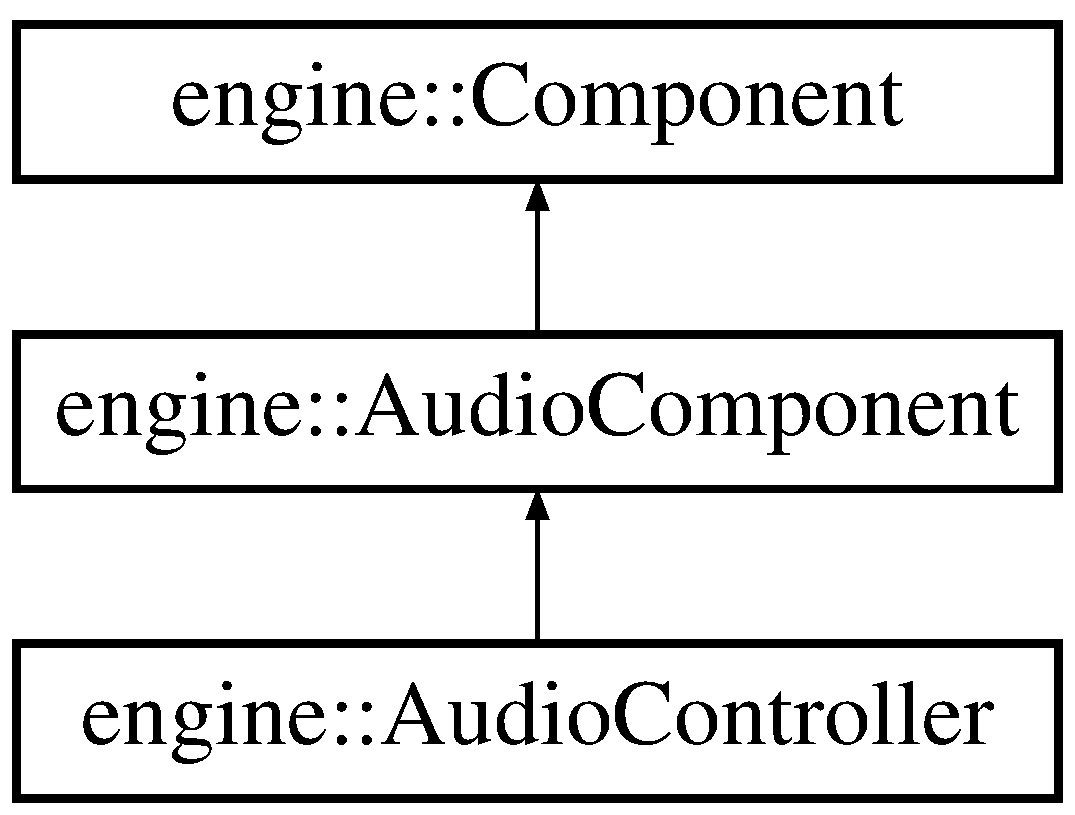
\includegraphics[height=3.000000cm]{classengine_1_1_audio_controller}
\end{center}
\end{figure}
\subsection*{Public Member Functions}
\begin{DoxyCompactItemize}
\item 
\hyperlink{classengine_1_1_audio_controller_ace94000a3e52f0473572395b0ef767a7}{Audio\+Controller} ()
\item 
virtual \hyperlink{classengine_1_1_audio_controller_afb803a7f9f6a450b13c73f972ecbd84d}{$\sim$\+Audio\+Controller} ()
\item 
\hyperlink{classengine_1_1_audio_controller_af8f485167b2b92c0bdd10e75b7f16e95}{Audio\+Controller} (\hyperlink{classengine_1_1_game_object}{Game\+Object} \&\hyperlink{classengine_1_1_component_ad4a4865ca4df98ebea34d04a4ec5ad07}{game\+Object})
\item 
void \hyperlink{classengine_1_1_audio_controller_a2ee4b9dd66a5ef288c22904267951dc1}{add\+Audio} (std\+::string audio\+Name, \hyperlink{classengine_1_1_audio_component}{Audio\+Component} \&audio)
\item 
void \hyperlink{classengine_1_1_audio_controller_a1c2527ac09312f27695a526d9888b420}{play\+Audio} (std\+::string audio\+Name)
\item 
void \hyperlink{classengine_1_1_audio_controller_ac065ab363d0494d376e9a50e558e52c6}{stop\+Audio} (std\+::string audio\+Name)
\item 
void \hyperlink{classengine_1_1_audio_controller_a230a285d71fbc1312b3fb4be9910182a}{pause\+Audio} (std\+::string audio\+Name)
\item 
void \hyperlink{classengine_1_1_audio_controller_a37c3410eaa94f29b465e29e72486a64d}{stop\+All\+Audios} ()
\item 
\hyperlink{namespaceengine_a5de9278ae356d4ff4fe8864ebf683bc8}{Audio\+State} \hyperlink{classengine_1_1_audio_controller_a72df19021e6d2bc8deb12ba35d7e6e8d}{get\+Audio\+State} (std\+::string audio\+Name)
\item 
void \hyperlink{classengine_1_1_audio_controller_a34af3c91cadbf4a97eafdd3e311671c9}{init} ()
\begin{DoxyCompactList}\small\item\em inherits function that initialize the game components \end{DoxyCompactList}\item 
void \hyperlink{classengine_1_1_audio_controller_aaeb8eaadaa523db5e3608f019fe1bf8e}{shutdown} ()
\begin{DoxyCompactList}\small\item\em inherits function that disable the game components \end{DoxyCompactList}\item 
void \hyperlink{classengine_1_1_audio_controller_acbbf0bd451c181fb1e3dc26e7c4be27d}{update\+Code} ()
\begin{DoxyCompactList}\small\item\em inherits function that update the game code. \end{DoxyCompactList}\end{DoxyCompactItemize}
\subsection*{Additional Inherited Members}


\subsection{Detailed Description}


Definition at line 26 of file audio\+\_\+controller.\+hpp.



\subsection{Constructor \& Destructor Documentation}
\index{engine\+::\+Audio\+Controller@{engine\+::\+Audio\+Controller}!Audio\+Controller@{Audio\+Controller}}
\index{Audio\+Controller@{Audio\+Controller}!engine\+::\+Audio\+Controller@{engine\+::\+Audio\+Controller}}
\subsubsection[{\texorpdfstring{Audio\+Controller()}{AudioController()}}]{\setlength{\rightskip}{0pt plus 5cm}Audio\+Controller\+::\+Audio\+Controller (
\begin{DoxyParamCaption}
{}
\end{DoxyParamCaption}
)}\hypertarget{classengine_1_1_audio_controller_ace94000a3e52f0473572395b0ef767a7}{}\label{classengine_1_1_audio_controller_ace94000a3e52f0473572395b0ef767a7}


Definition at line 52 of file audio\+\_\+controller.\+cpp.

\index{engine\+::\+Audio\+Controller@{engine\+::\+Audio\+Controller}!````~Audio\+Controller@{$\sim$\+Audio\+Controller}}
\index{````~Audio\+Controller@{$\sim$\+Audio\+Controller}!engine\+::\+Audio\+Controller@{engine\+::\+Audio\+Controller}}
\subsubsection[{\texorpdfstring{$\sim$\+Audio\+Controller()}{~AudioController()}}]{\setlength{\rightskip}{0pt plus 5cm}Audio\+Controller\+::$\sim$\+Audio\+Controller (
\begin{DoxyParamCaption}
{}
\end{DoxyParamCaption}
)\hspace{0.3cm}{\ttfamily [virtual]}}\hypertarget{classengine_1_1_audio_controller_afb803a7f9f6a450b13c73f972ecbd84d}{}\label{classengine_1_1_audio_controller_afb803a7f9f6a450b13c73f972ecbd84d}


Definition at line 14 of file audio\+\_\+controller.\+cpp.

\index{engine\+::\+Audio\+Controller@{engine\+::\+Audio\+Controller}!Audio\+Controller@{Audio\+Controller}}
\index{Audio\+Controller@{Audio\+Controller}!engine\+::\+Audio\+Controller@{engine\+::\+Audio\+Controller}}
\subsubsection[{\texorpdfstring{Audio\+Controller(\+Game\+Object \&game\+Object)}{AudioController(GameObject &gameObject)}}]{\setlength{\rightskip}{0pt plus 5cm}Audio\+Controller\+::\+Audio\+Controller (
\begin{DoxyParamCaption}
\item[{{\bf Game\+Object} \&}]{game\+Object}
\end{DoxyParamCaption}
)}\hypertarget{classengine_1_1_audio_controller_af8f485167b2b92c0bdd10e75b7f16e95}{}\label{classengine_1_1_audio_controller_af8f485167b2b92c0bdd10e75b7f16e95}


Definition at line 61 of file audio\+\_\+controller.\+cpp.



\subsection{Member Function Documentation}
\index{engine\+::\+Audio\+Controller@{engine\+::\+Audio\+Controller}!add\+Audio@{add\+Audio}}
\index{add\+Audio@{add\+Audio}!engine\+::\+Audio\+Controller@{engine\+::\+Audio\+Controller}}
\subsubsection[{\texorpdfstring{add\+Audio(std\+::string audio\+Name, Audio\+Component \&audio)}{addAudio(std::string audioName, AudioComponent &audio)}}]{\setlength{\rightskip}{0pt plus 5cm}void Audio\+Controller\+::add\+Audio (
\begin{DoxyParamCaption}
\item[{std\+::string}]{audio\+Name, }
\item[{{\bf Audio\+Component} \&}]{audio}
\end{DoxyParamCaption}
)}\hypertarget{classengine_1_1_audio_controller_a2ee4b9dd66a5ef288c22904267951dc1}{}\label{classengine_1_1_audio_controller_a2ee4b9dd66a5ef288c22904267951dc1}


Definition at line 71 of file audio\+\_\+controller.\+cpp.

\index{engine\+::\+Audio\+Controller@{engine\+::\+Audio\+Controller}!get\+Audio\+State@{get\+Audio\+State}}
\index{get\+Audio\+State@{get\+Audio\+State}!engine\+::\+Audio\+Controller@{engine\+::\+Audio\+Controller}}
\subsubsection[{\texorpdfstring{get\+Audio\+State(std\+::string audio\+Name)}{getAudioState(std::string audioName)}}]{\setlength{\rightskip}{0pt plus 5cm}{\bf Audio\+State} Audio\+Controller\+::get\+Audio\+State (
\begin{DoxyParamCaption}
\item[{std\+::string}]{audio\+Name}
\end{DoxyParamCaption}
)}\hypertarget{classengine_1_1_audio_controller_a72df19021e6d2bc8deb12ba35d7e6e8d}{}\label{classengine_1_1_audio_controller_a72df19021e6d2bc8deb12ba35d7e6e8d}


Definition at line 134 of file audio\+\_\+controller.\+cpp.

\index{engine\+::\+Audio\+Controller@{engine\+::\+Audio\+Controller}!init@{init}}
\index{init@{init}!engine\+::\+Audio\+Controller@{engine\+::\+Audio\+Controller}}
\subsubsection[{\texorpdfstring{init()}{init()}}]{\setlength{\rightskip}{0pt plus 5cm}void Audio\+Controller\+::init (
\begin{DoxyParamCaption}
{}
\end{DoxyParamCaption}
)\hspace{0.3cm}{\ttfamily [virtual]}}\hypertarget{classengine_1_1_audio_controller_a34af3c91cadbf4a97eafdd3e311671c9}{}\label{classengine_1_1_audio_controller_a34af3c91cadbf4a97eafdd3e311671c9}


inherits function that initialize the game components 

Set all game components to enable

\begin{DoxyReturn}{Returns}
\char`\"{}void\char`\"{}. 
\end{DoxyReturn}


Reimplemented from \hyperlink{classengine_1_1_audio_component_a61f7e9f09253a0619ed979276267150c}{engine\+::\+Audio\+Component}.



Definition at line 19 of file audio\+\_\+controller.\+cpp.

\index{engine\+::\+Audio\+Controller@{engine\+::\+Audio\+Controller}!pause\+Audio@{pause\+Audio}}
\index{pause\+Audio@{pause\+Audio}!engine\+::\+Audio\+Controller@{engine\+::\+Audio\+Controller}}
\subsubsection[{\texorpdfstring{pause\+Audio(std\+::string audio\+Name)}{pauseAudio(std::string audioName)}}]{\setlength{\rightskip}{0pt plus 5cm}void Audio\+Controller\+::pause\+Audio (
\begin{DoxyParamCaption}
\item[{std\+::string}]{audio\+Name}
\end{DoxyParamCaption}
)}\hypertarget{classengine_1_1_audio_controller_a230a285d71fbc1312b3fb4be9910182a}{}\label{classengine_1_1_audio_controller_a230a285d71fbc1312b3fb4be9910182a}


Definition at line 118 of file audio\+\_\+controller.\+cpp.

\index{engine\+::\+Audio\+Controller@{engine\+::\+Audio\+Controller}!play\+Audio@{play\+Audio}}
\index{play\+Audio@{play\+Audio}!engine\+::\+Audio\+Controller@{engine\+::\+Audio\+Controller}}
\subsubsection[{\texorpdfstring{play\+Audio(std\+::string audio\+Name)}{playAudio(std::string audioName)}}]{\setlength{\rightskip}{0pt plus 5cm}void Audio\+Controller\+::play\+Audio (
\begin{DoxyParamCaption}
\item[{std\+::string}]{audio\+Name}
\end{DoxyParamCaption}
)}\hypertarget{classengine_1_1_audio_controller_a1c2527ac09312f27695a526d9888b420}{}\label{classengine_1_1_audio_controller_a1c2527ac09312f27695a526d9888b420}


Definition at line 80 of file audio\+\_\+controller.\+cpp.

\index{engine\+::\+Audio\+Controller@{engine\+::\+Audio\+Controller}!shutdown@{shutdown}}
\index{shutdown@{shutdown}!engine\+::\+Audio\+Controller@{engine\+::\+Audio\+Controller}}
\subsubsection[{\texorpdfstring{shutdown()}{shutdown()}}]{\setlength{\rightskip}{0pt plus 5cm}void Audio\+Controller\+::shutdown (
\begin{DoxyParamCaption}
{}
\end{DoxyParamCaption}
)\hspace{0.3cm}{\ttfamily [virtual]}}\hypertarget{classengine_1_1_audio_controller_aaeb8eaadaa523db5e3608f019fe1bf8e}{}\label{classengine_1_1_audio_controller_aaeb8eaadaa523db5e3608f019fe1bf8e}


inherits function that disable the game components 

free the component pointers

\begin{DoxyReturn}{Returns}
\char`\"{}void\char`\"{}. 
\end{DoxyReturn}


Reimplemented from \hyperlink{classengine_1_1_audio_component_acb42c8fa38793ff0fe6c0652bbb9eac9}{engine\+::\+Audio\+Component}.



Definition at line 31 of file audio\+\_\+controller.\+cpp.

\index{engine\+::\+Audio\+Controller@{engine\+::\+Audio\+Controller}!stop\+All\+Audios@{stop\+All\+Audios}}
\index{stop\+All\+Audios@{stop\+All\+Audios}!engine\+::\+Audio\+Controller@{engine\+::\+Audio\+Controller}}
\subsubsection[{\texorpdfstring{stop\+All\+Audios()}{stopAllAudios()}}]{\setlength{\rightskip}{0pt plus 5cm}void Audio\+Controller\+::stop\+All\+Audios (
\begin{DoxyParamCaption}
{}
\end{DoxyParamCaption}
)}\hypertarget{classengine_1_1_audio_controller_a37c3410eaa94f29b465e29e72486a64d}{}\label{classengine_1_1_audio_controller_a37c3410eaa94f29b465e29e72486a64d}


Definition at line 108 of file audio\+\_\+controller.\+cpp.

\index{engine\+::\+Audio\+Controller@{engine\+::\+Audio\+Controller}!stop\+Audio@{stop\+Audio}}
\index{stop\+Audio@{stop\+Audio}!engine\+::\+Audio\+Controller@{engine\+::\+Audio\+Controller}}
\subsubsection[{\texorpdfstring{stop\+Audio(std\+::string audio\+Name)}{stopAudio(std::string audioName)}}]{\setlength{\rightskip}{0pt plus 5cm}void Audio\+Controller\+::stop\+Audio (
\begin{DoxyParamCaption}
\item[{std\+::string}]{audio\+Name}
\end{DoxyParamCaption}
)}\hypertarget{classengine_1_1_audio_controller_ac065ab363d0494d376e9a50e558e52c6}{}\label{classengine_1_1_audio_controller_ac065ab363d0494d376e9a50e558e52c6}


Definition at line 97 of file audio\+\_\+controller.\+cpp.

\index{engine\+::\+Audio\+Controller@{engine\+::\+Audio\+Controller}!update\+Code@{update\+Code}}
\index{update\+Code@{update\+Code}!engine\+::\+Audio\+Controller@{engine\+::\+Audio\+Controller}}
\subsubsection[{\texorpdfstring{update\+Code()}{updateCode()}}]{\setlength{\rightskip}{0pt plus 5cm}void Audio\+Controller\+::update\+Code (
\begin{DoxyParamCaption}
{}
\end{DoxyParamCaption}
)\hspace{0.3cm}{\ttfamily [virtual]}}\hypertarget{classengine_1_1_audio_controller_acbbf0bd451c181fb1e3dc26e7c4be27d}{}\label{classengine_1_1_audio_controller_acbbf0bd451c181fb1e3dc26e7c4be27d}


inherits function that update the game code. 

update all the enabled game objects.

\begin{DoxyReturn}{Returns}
\char`\"{}void\char`\"{}. 
\end{DoxyReturn}


Reimplemented from \hyperlink{classengine_1_1_audio_component_aa35e7f57c104c2281680bb13764e4ef0}{engine\+::\+Audio\+Component}.



Definition at line 40 of file audio\+\_\+controller.\+cpp.



The documentation for this class was generated from the following files\+:\begin{DoxyCompactItemize}
\item 
engine/include/\hyperlink{audio__controller_8hpp}{audio\+\_\+controller.\+hpp}\item 
engine/src/\hyperlink{audio__controller_8cpp}{audio\+\_\+controller.\+cpp}\end{DoxyCompactItemize}

\hypertarget{classengine_1_1_background_component}{}\section{engine\+:\+:Background\+Component Class Reference}
\label{classengine_1_1_background_component}\index{engine\+::\+Background\+Component@{engine\+::\+Background\+Component}}


{\ttfamily \#include $<$background\+\_\+component.\+hpp$>$}

Inheritance diagram for engine\+:\+:Background\+Component\+:\begin{figure}[H]
\begin{center}
\leavevmode
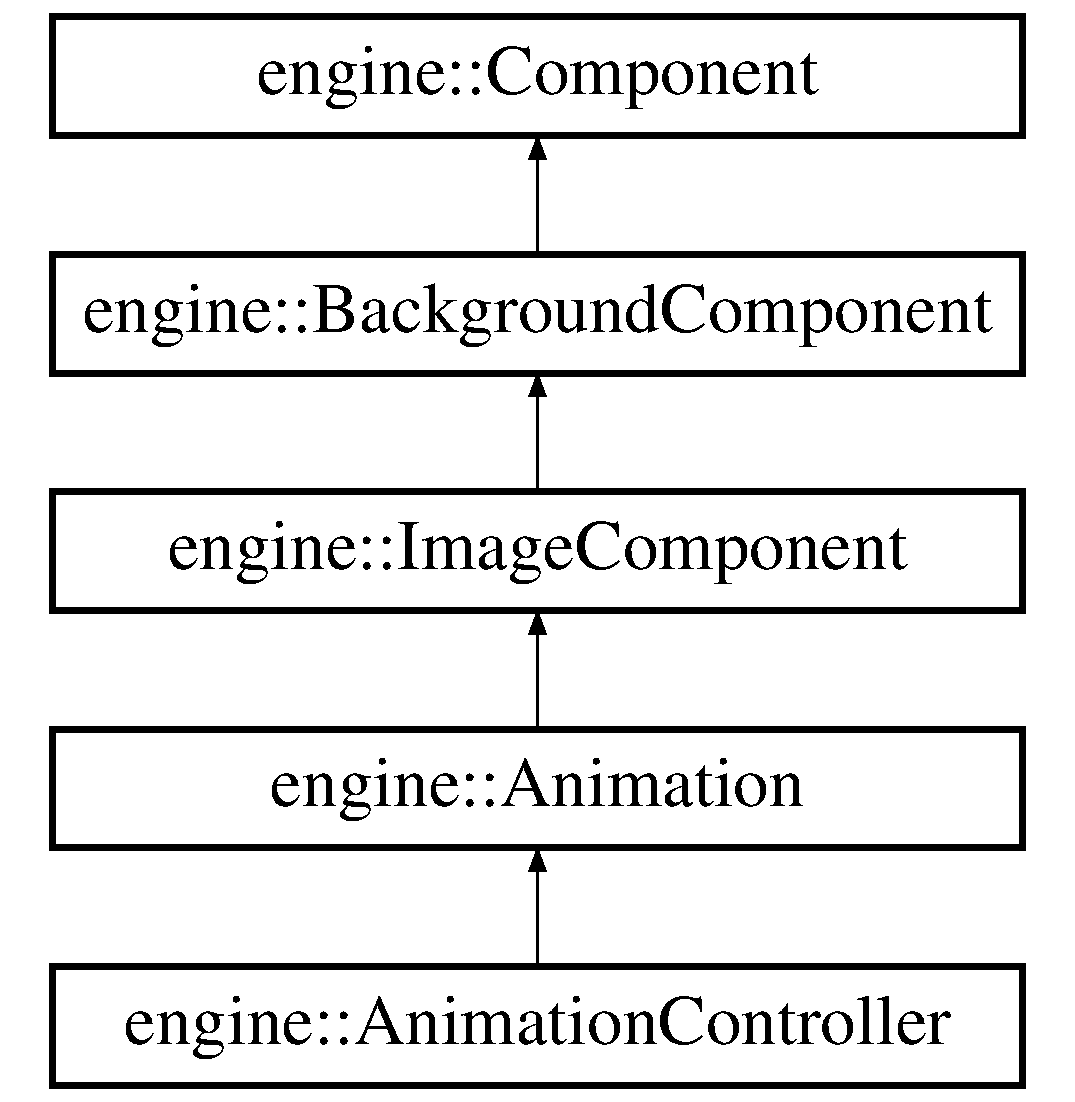
\includegraphics[height=5.000000cm]{classengine_1_1_background_component}
\end{center}
\end{figure}
\subsection*{Public Member Functions}
\begin{DoxyCompactItemize}
\item 
\hyperlink{classengine_1_1_background_component_a80e304ab2a7f912dc7947645e26ff992}{Background\+Component} ()
\item 
\hyperlink{classengine_1_1_background_component_aba5db2cc51b47dc1fcf48a253cb37e79}{Background\+Component} (std\+::string \hyperlink{classengine_1_1_background_component_aeffcb1aa8b67444e004413dee8c266b1}{image\+Path})
\item 
\hyperlink{classengine_1_1_background_component_a0ec590cdd404d4fbf106b7c14a6a7260}{Background\+Component} (\hyperlink{classengine_1_1_game_object}{Game\+Object} \&\hyperlink{classengine_1_1_component_ad4a4865ca4df98ebea34d04a4ec5ad07}{game\+Object}, std\+::string \hyperlink{classengine_1_1_background_component_aeffcb1aa8b67444e004413dee8c266b1}{image\+Path})
\item 
\hyperlink{classengine_1_1_background_component_a2de1b03eff649102040132d22f6e23e1}{$\sim$\+Background\+Component} ()
\item 
void \hyperlink{classengine_1_1_background_component_a88a96b265f85934474d23d37cb2e6413}{init} ()
\begin{DoxyCompactList}\small\item\em inherits function that initialize the game components \end{DoxyCompactList}\item 
void \hyperlink{classengine_1_1_background_component_a88da6fd205007306776b1ff186b29668}{shutdown} ()
\begin{DoxyCompactList}\small\item\em inherits function that disable the game components \end{DoxyCompactList}\item 
void \hyperlink{classengine_1_1_background_component_a7b3c366c4b917888bde48917d83994be}{draw} ()
\begin{DoxyCompactList}\small\item\em inherits function that draw game objects. \end{DoxyCompactList}\item 
std\+::string \hyperlink{classengine_1_1_background_component_ad3283bbe6ab2d5c170ca67d2180c9fe2}{get\+Class\+Name} ()
\begin{DoxyCompactList}\small\item\em access the name of the class. \end{DoxyCompactList}\end{DoxyCompactItemize}
\subsection*{Protected Attributes}
\begin{DoxyCompactItemize}
\item 
std\+::string \hyperlink{classengine_1_1_background_component_aeffcb1aa8b67444e004413dee8c266b1}{image\+Path}
\item 
S\+D\+L\+\_\+\+Texture $\ast$ \hyperlink{classengine_1_1_background_component_a8f3e8087b12106e4cea2f3c3c5e75c8e}{image\+Texture}
\item 
S\+D\+L\+\_\+\+Rect \hyperlink{classengine_1_1_background_component_afade3c167174d12a54b2b548199c3942}{render\+Quad}
\item 
int \hyperlink{classengine_1_1_background_component_ab791d4b2d6c30affd8d27bbd2f51db69}{component\+Width}
\item 
int \hyperlink{classengine_1_1_background_component_af3aa1860b46dc7d4d1252c2a62d03f24}{component\+Height}
\end{DoxyCompactItemize}


\subsection{Detailed Description}


Definition at line 25 of file background\+\_\+component.\+hpp.



\subsection{Constructor \& Destructor Documentation}
\index{engine\+::\+Background\+Component@{engine\+::\+Background\+Component}!Background\+Component@{Background\+Component}}
\index{Background\+Component@{Background\+Component}!engine\+::\+Background\+Component@{engine\+::\+Background\+Component}}
\subsubsection[{\texorpdfstring{Background\+Component()}{BackgroundComponent()}}]{\setlength{\rightskip}{0pt plus 5cm}Background\+Component\+::\+Background\+Component (
\begin{DoxyParamCaption}
{}
\end{DoxyParamCaption}
)}\hypertarget{classengine_1_1_background_component_a80e304ab2a7f912dc7947645e26ff992}{}\label{classengine_1_1_background_component_a80e304ab2a7f912dc7947645e26ff992}


Definition at line 23 of file background\+\_\+component.\+cpp.

\index{engine\+::\+Background\+Component@{engine\+::\+Background\+Component}!Background\+Component@{Background\+Component}}
\index{Background\+Component@{Background\+Component}!engine\+::\+Background\+Component@{engine\+::\+Background\+Component}}
\subsubsection[{\texorpdfstring{Background\+Component(std\+::string image\+Path)}{BackgroundComponent(std::string imagePath)}}]{\setlength{\rightskip}{0pt plus 5cm}Background\+Component\+::\+Background\+Component (
\begin{DoxyParamCaption}
\item[{std\+::string}]{image\+Path}
\end{DoxyParamCaption}
)}\hypertarget{classengine_1_1_background_component_aba5db2cc51b47dc1fcf48a253cb37e79}{}\label{classengine_1_1_background_component_aba5db2cc51b47dc1fcf48a253cb37e79}


Definition at line 25 of file background\+\_\+component.\+cpp.

\index{engine\+::\+Background\+Component@{engine\+::\+Background\+Component}!Background\+Component@{Background\+Component}}
\index{Background\+Component@{Background\+Component}!engine\+::\+Background\+Component@{engine\+::\+Background\+Component}}
\subsubsection[{\texorpdfstring{Background\+Component(\+Game\+Object \&game\+Object, std\+::string image\+Path)}{BackgroundComponent(GameObject &gameObject, std::string imagePath)}}]{\setlength{\rightskip}{0pt plus 5cm}Background\+Component\+::\+Background\+Component (
\begin{DoxyParamCaption}
\item[{{\bf Game\+Object} \&}]{game\+Object, }
\item[{std\+::string}]{image\+Path}
\end{DoxyParamCaption}
)}\hypertarget{classengine_1_1_background_component_a0ec590cdd404d4fbf106b7c14a6a7260}{}\label{classengine_1_1_background_component_a0ec590cdd404d4fbf106b7c14a6a7260}


Definition at line 30 of file background\+\_\+component.\+cpp.

\index{engine\+::\+Background\+Component@{engine\+::\+Background\+Component}!````~Background\+Component@{$\sim$\+Background\+Component}}
\index{````~Background\+Component@{$\sim$\+Background\+Component}!engine\+::\+Background\+Component@{engine\+::\+Background\+Component}}
\subsubsection[{\texorpdfstring{$\sim$\+Background\+Component()}{~BackgroundComponent()}}]{\setlength{\rightskip}{0pt plus 5cm}Background\+Component\+::$\sim$\+Background\+Component (
\begin{DoxyParamCaption}
{}
\end{DoxyParamCaption}
)}\hypertarget{classengine_1_1_background_component_a2de1b03eff649102040132d22f6e23e1}{}\label{classengine_1_1_background_component_a2de1b03eff649102040132d22f6e23e1}


Definition at line 36 of file background\+\_\+component.\+cpp.



\subsection{Member Function Documentation}
\index{engine\+::\+Background\+Component@{engine\+::\+Background\+Component}!draw@{draw}}
\index{draw@{draw}!engine\+::\+Background\+Component@{engine\+::\+Background\+Component}}
\subsubsection[{\texorpdfstring{draw()}{draw()}}]{\setlength{\rightskip}{0pt plus 5cm}void Background\+Component\+::draw (
\begin{DoxyParamCaption}
{}
\end{DoxyParamCaption}
)\hspace{0.3cm}{\ttfamily [virtual]}}\hypertarget{classengine_1_1_background_component_a7b3c366c4b917888bde48917d83994be}{}\label{classengine_1_1_background_component_a7b3c366c4b917888bde48917d83994be}


inherits function that draw game objects. 

draws all the enabled game objects.

\begin{DoxyReturn}{Returns}
\char`\"{}void\char`\"{}. 
\end{DoxyReturn}


Reimplemented from \hyperlink{classengine_1_1_component_a3d20060d4af0bf0dd0c833994581bdfa}{engine\+::\+Component}.



Reimplemented in \hyperlink{classengine_1_1_image_component_a2be1a46da22f0f2280f7748c49fa6276}{engine\+::\+Image\+Component}.



Definition at line 52 of file background\+\_\+component.\+cpp.

\index{engine\+::\+Background\+Component@{engine\+::\+Background\+Component}!get\+Class\+Name@{get\+Class\+Name}}
\index{get\+Class\+Name@{get\+Class\+Name}!engine\+::\+Background\+Component@{engine\+::\+Background\+Component}}
\subsubsection[{\texorpdfstring{get\+Class\+Name()}{getClassName()}}]{\setlength{\rightskip}{0pt plus 5cm}std\+::string engine\+::\+Background\+Component\+::get\+Class\+Name (
\begin{DoxyParamCaption}
{}
\end{DoxyParamCaption}
)\hspace{0.3cm}{\ttfamily [inline]}, {\ttfamily [virtual]}}\hypertarget{classengine_1_1_background_component_ad3283bbe6ab2d5c170ca67d2180c9fe2}{}\label{classengine_1_1_background_component_ad3283bbe6ab2d5c170ca67d2180c9fe2}


access the name of the class. 

Used to get the private attribute class\+Name.

\begin{DoxyReturn}{Returns}
string that contains the scene name. 
\end{DoxyReturn}


Reimplemented from \hyperlink{classengine_1_1_component_a4341ed3c744b160590908bea151b6ca7}{engine\+::\+Component}.



Reimplemented in \hyperlink{classengine_1_1_image_component_ac18bc924683d4d389b6706abd0afab20}{engine\+::\+Image\+Component}.



Definition at line 40 of file background\+\_\+component.\+hpp.

\index{engine\+::\+Background\+Component@{engine\+::\+Background\+Component}!init@{init}}
\index{init@{init}!engine\+::\+Background\+Component@{engine\+::\+Background\+Component}}
\subsubsection[{\texorpdfstring{init()}{init()}}]{\setlength{\rightskip}{0pt plus 5cm}void Background\+Component\+::init (
\begin{DoxyParamCaption}
{}
\end{DoxyParamCaption}
)\hspace{0.3cm}{\ttfamily [virtual]}}\hypertarget{classengine_1_1_background_component_a88a96b265f85934474d23d37cb2e6413}{}\label{classengine_1_1_background_component_a88a96b265f85934474d23d37cb2e6413}


inherits function that initialize the game components 

Set all game components to enable

\begin{DoxyReturn}{Returns}
\char`\"{}void\char`\"{}. 
\end{DoxyReturn}


Reimplemented from \hyperlink{classengine_1_1_component_aa0bf4fb5f4bc0de25d3f7beef3a3ca45}{engine\+::\+Component}.



Reimplemented in \hyperlink{classengine_1_1_image_component_a4e5def28ca4647b29a4fe9bda78f9e57}{engine\+::\+Image\+Component}.



Definition at line 38 of file background\+\_\+component.\+cpp.

\index{engine\+::\+Background\+Component@{engine\+::\+Background\+Component}!shutdown@{shutdown}}
\index{shutdown@{shutdown}!engine\+::\+Background\+Component@{engine\+::\+Background\+Component}}
\subsubsection[{\texorpdfstring{shutdown()}{shutdown()}}]{\setlength{\rightskip}{0pt plus 5cm}void Background\+Component\+::shutdown (
\begin{DoxyParamCaption}
{}
\end{DoxyParamCaption}
)\hspace{0.3cm}{\ttfamily [virtual]}}\hypertarget{classengine_1_1_background_component_a88da6fd205007306776b1ff186b29668}{}\label{classengine_1_1_background_component_a88da6fd205007306776b1ff186b29668}


inherits function that disable the game components 

free the component pointers

\begin{DoxyReturn}{Returns}
\char`\"{}void\char`\"{}. 
\end{DoxyReturn}


Reimplemented from \hyperlink{classengine_1_1_component_a3e47775d51e78914bdfebba123354849}{engine\+::\+Component}.



Definition at line 47 of file background\+\_\+component.\+cpp.



\subsection{Member Data Documentation}
\index{engine\+::\+Background\+Component@{engine\+::\+Background\+Component}!component\+Height@{component\+Height}}
\index{component\+Height@{component\+Height}!engine\+::\+Background\+Component@{engine\+::\+Background\+Component}}
\subsubsection[{\texorpdfstring{component\+Height}{componentHeight}}]{\setlength{\rightskip}{0pt plus 5cm}int engine\+::\+Background\+Component\+::component\+Height\hspace{0.3cm}{\ttfamily [protected]}}\hypertarget{classengine_1_1_background_component_af3aa1860b46dc7d4d1252c2a62d03f24}{}\label{classengine_1_1_background_component_af3aa1860b46dc7d4d1252c2a62d03f24}


Definition at line 31 of file background\+\_\+component.\+hpp.

\index{engine\+::\+Background\+Component@{engine\+::\+Background\+Component}!component\+Width@{component\+Width}}
\index{component\+Width@{component\+Width}!engine\+::\+Background\+Component@{engine\+::\+Background\+Component}}
\subsubsection[{\texorpdfstring{component\+Width}{componentWidth}}]{\setlength{\rightskip}{0pt plus 5cm}int engine\+::\+Background\+Component\+::component\+Width\hspace{0.3cm}{\ttfamily [protected]}}\hypertarget{classengine_1_1_background_component_ab791d4b2d6c30affd8d27bbd2f51db69}{}\label{classengine_1_1_background_component_ab791d4b2d6c30affd8d27bbd2f51db69}


Definition at line 30 of file background\+\_\+component.\+hpp.

\index{engine\+::\+Background\+Component@{engine\+::\+Background\+Component}!image\+Path@{image\+Path}}
\index{image\+Path@{image\+Path}!engine\+::\+Background\+Component@{engine\+::\+Background\+Component}}
\subsubsection[{\texorpdfstring{image\+Path}{imagePath}}]{\setlength{\rightskip}{0pt plus 5cm}std\+::string engine\+::\+Background\+Component\+::image\+Path\hspace{0.3cm}{\ttfamily [protected]}}\hypertarget{classengine_1_1_background_component_aeffcb1aa8b67444e004413dee8c266b1}{}\label{classengine_1_1_background_component_aeffcb1aa8b67444e004413dee8c266b1}


Definition at line 27 of file background\+\_\+component.\+hpp.

\index{engine\+::\+Background\+Component@{engine\+::\+Background\+Component}!image\+Texture@{image\+Texture}}
\index{image\+Texture@{image\+Texture}!engine\+::\+Background\+Component@{engine\+::\+Background\+Component}}
\subsubsection[{\texorpdfstring{image\+Texture}{imageTexture}}]{\setlength{\rightskip}{0pt plus 5cm}S\+D\+L\+\_\+\+Texture$\ast$ engine\+::\+Background\+Component\+::image\+Texture\hspace{0.3cm}{\ttfamily [protected]}}\hypertarget{classengine_1_1_background_component_a8f3e8087b12106e4cea2f3c3c5e75c8e}{}\label{classengine_1_1_background_component_a8f3e8087b12106e4cea2f3c3c5e75c8e}


Definition at line 28 of file background\+\_\+component.\+hpp.

\index{engine\+::\+Background\+Component@{engine\+::\+Background\+Component}!render\+Quad@{render\+Quad}}
\index{render\+Quad@{render\+Quad}!engine\+::\+Background\+Component@{engine\+::\+Background\+Component}}
\subsubsection[{\texorpdfstring{render\+Quad}{renderQuad}}]{\setlength{\rightskip}{0pt plus 5cm}S\+D\+L\+\_\+\+Rect engine\+::\+Background\+Component\+::render\+Quad\hspace{0.3cm}{\ttfamily [protected]}}\hypertarget{classengine_1_1_background_component_afade3c167174d12a54b2b548199c3942}{}\label{classengine_1_1_background_component_afade3c167174d12a54b2b548199c3942}


Definition at line 29 of file background\+\_\+component.\+hpp.



The documentation for this class was generated from the following files\+:\begin{DoxyCompactItemize}
\item 
engine/include/\hyperlink{background__component_8hpp}{background\+\_\+component.\+hpp}\item 
engine/src/\hyperlink{background__component_8cpp}{background\+\_\+component.\+cpp}\end{DoxyCompactItemize}

\hypertarget{classengine_1_1_code_component}{}\section{engine\+:\+:Code\+Component Class Reference}
\label{classengine_1_1_code_component}\index{engine\+::\+Code\+Component@{engine\+::\+Code\+Component}}


A Code \hyperlink{classengine_1_1_component}{Component} class.  




{\ttfamily \#include $<$code\+\_\+component.\+hpp$>$}

Inheritance diagram for engine\+:\+:Code\+Component\+:\begin{figure}[H]
\begin{center}
\leavevmode
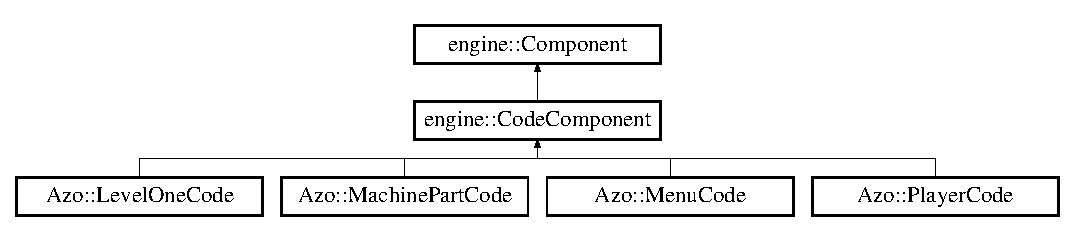
\includegraphics[height=2.675159cm]{classengine_1_1_code_component}
\end{center}
\end{figure}
\subsection*{Public Member Functions}
\begin{DoxyCompactItemize}
\item 
\hyperlink{classengine_1_1_code_component_a7dada09414813e7a5f83679323402dd3}{Code\+Component} ()
\begin{DoxyCompactList}\small\item\em Default constructor for the code component. \end{DoxyCompactList}\item 
\hyperlink{classengine_1_1_code_component_aa48bca8c3008c5d51e5131dde228deb3}{Code\+Component} (\hyperlink{classengine_1_1_game_object}{Game\+Object} \&\hyperlink{classengine_1_1_component_ad4a4865ca4df98ebea34d04a4ec5ad07}{game\+Object})
\begin{DoxyCompactList}\small\item\em Constructor for the code component. \end{DoxyCompactList}\item 
void \hyperlink{classengine_1_1_code_component_a710d9f79114c7b055aaa94fae179ae55}{init} ()
\begin{DoxyCompactList}\small\item\em inherits function that initialize the game code components. \end{DoxyCompactList}\item 
void \hyperlink{classengine_1_1_code_component_af76ba17f9f87216418081d1e2c7c3a22}{shutdown} ()
\begin{DoxyCompactList}\small\item\em inherits function that disable the game code components. \end{DoxyCompactList}\item 
void \hyperlink{classengine_1_1_code_component_a78363275025956ccdbfa11fd42f8ae96}{update\+Code} ()
\begin{DoxyCompactList}\small\item\em inherits function that update the game code. \end{DoxyCompactList}\end{DoxyCompactItemize}
\subsection*{Additional Inherited Members}


\subsection{Detailed Description}
A Code \hyperlink{classengine_1_1_component}{Component} class. 

Generic \hyperlink{classengine_1_1_component}{Component} class. It\textquotesingle{}s how the engine\textquotesingle{}ll see all components that will try to use it. 

Definition at line 30 of file code\+\_\+component.\+hpp.



\subsection{Constructor \& Destructor Documentation}
\index{engine\+::\+Code\+Component@{engine\+::\+Code\+Component}!Code\+Component@{Code\+Component}}
\index{Code\+Component@{Code\+Component}!engine\+::\+Code\+Component@{engine\+::\+Code\+Component}}
\subsubsection[{\texorpdfstring{Code\+Component()}{CodeComponent()}}]{\setlength{\rightskip}{0pt plus 5cm}Code\+Component\+::\+Code\+Component (
\begin{DoxyParamCaption}
{}
\end{DoxyParamCaption}
)}\hypertarget{classengine_1_1_code_component_a7dada09414813e7a5f83679323402dd3}{}\label{classengine_1_1_code_component_a7dada09414813e7a5f83679323402dd3}


Default constructor for the code component. 

\begin{DoxyReturn}{Returns}
\char`\"{}void\char`\"{}. 
\end{DoxyReturn}


Definition at line 22 of file code\+\_\+component.\+cpp.

\index{engine\+::\+Code\+Component@{engine\+::\+Code\+Component}!Code\+Component@{Code\+Component}}
\index{Code\+Component@{Code\+Component}!engine\+::\+Code\+Component@{engine\+::\+Code\+Component}}
\subsubsection[{\texorpdfstring{Code\+Component(\+Game\+Object \&game\+Object)}{CodeComponent(GameObject &gameObject)}}]{\setlength{\rightskip}{0pt plus 5cm}Code\+Component\+::\+Code\+Component (
\begin{DoxyParamCaption}
\item[{{\bf Game\+Object} \&}]{game\+Object}
\end{DoxyParamCaption}
)}\hypertarget{classengine_1_1_code_component_aa48bca8c3008c5d51e5131dde228deb3}{}\label{classengine_1_1_code_component_aa48bca8c3008c5d51e5131dde228deb3}


Constructor for the code component. 


\begin{DoxyParams}{Parameters}
{\em game} & object to the code component.\\
\hline
\end{DoxyParams}
\begin{DoxyReturn}{Returns}
\char`\"{}void\char`\"{}. 
\end{DoxyReturn}


Definition at line 31 of file code\+\_\+component.\+cpp.



\subsection{Member Function Documentation}
\index{engine\+::\+Code\+Component@{engine\+::\+Code\+Component}!init@{init}}
\index{init@{init}!engine\+::\+Code\+Component@{engine\+::\+Code\+Component}}
\subsubsection[{\texorpdfstring{init()}{init()}}]{\setlength{\rightskip}{0pt plus 5cm}void Code\+Component\+::init (
\begin{DoxyParamCaption}
{}
\end{DoxyParamCaption}
)\hspace{0.3cm}{\ttfamily [virtual]}}\hypertarget{classengine_1_1_code_component_a710d9f79114c7b055aaa94fae179ae55}{}\label{classengine_1_1_code_component_a710d9f79114c7b055aaa94fae179ae55}


inherits function that initialize the game code components. 

Set all game code components to enable.

\begin{DoxyReturn}{Returns}
\char`\"{}void\char`\"{}. 
\end{DoxyReturn}


Reimplemented from \hyperlink{classengine_1_1_component_aa0bf4fb5f4bc0de25d3f7beef3a3ca45}{engine\+::\+Component}.



Definition at line 43 of file code\+\_\+component.\+cpp.

\index{engine\+::\+Code\+Component@{engine\+::\+Code\+Component}!shutdown@{shutdown}}
\index{shutdown@{shutdown}!engine\+::\+Code\+Component@{engine\+::\+Code\+Component}}
\subsubsection[{\texorpdfstring{shutdown()}{shutdown()}}]{\setlength{\rightskip}{0pt plus 5cm}void Code\+Component\+::shutdown (
\begin{DoxyParamCaption}
{}
\end{DoxyParamCaption}
)\hspace{0.3cm}{\ttfamily [virtual]}}\hypertarget{classengine_1_1_code_component_af76ba17f9f87216418081d1e2c7c3a22}{}\label{classengine_1_1_code_component_af76ba17f9f87216418081d1e2c7c3a22}


inherits function that disable the game code components. 

free the code component pointer.

\begin{DoxyReturn}{Returns}
\char`\"{}void\char`\"{}. 
\end{DoxyReturn}


Reimplemented from \hyperlink{classengine_1_1_component_a3e47775d51e78914bdfebba123354849}{engine\+::\+Component}.



Reimplemented in \hyperlink{class_azo_1_1_player_code_aea1004e3e9f7c7c58d69f428dd0b5b6f}{Azo\+::\+Player\+Code}, \hyperlink{class_azo_1_1_level_one_code_af66d92f836d8a6c0f72d718d05db63a5}{Azo\+::\+Level\+One\+Code}, and \hyperlink{class_azo_1_1_machine_part_code_aea9e8e5ccc20e0ac975277104b29d0bf}{Azo\+::\+Machine\+Part\+Code}.



Definition at line 52 of file code\+\_\+component.\+cpp.

\index{engine\+::\+Code\+Component@{engine\+::\+Code\+Component}!update\+Code@{update\+Code}}
\index{update\+Code@{update\+Code}!engine\+::\+Code\+Component@{engine\+::\+Code\+Component}}
\subsubsection[{\texorpdfstring{update\+Code()}{updateCode()}}]{\setlength{\rightskip}{0pt plus 5cm}void Code\+Component\+::update\+Code (
\begin{DoxyParamCaption}
{}
\end{DoxyParamCaption}
)\hspace{0.3cm}{\ttfamily [virtual]}}\hypertarget{classengine_1_1_code_component_a78363275025956ccdbfa11fd42f8ae96}{}\label{classengine_1_1_code_component_a78363275025956ccdbfa11fd42f8ae96}


inherits function that update the game code. 

update all the enabled game objects.

\begin{DoxyReturn}{Returns}
\char`\"{}void\char`\"{}. 
\end{DoxyReturn}


Reimplemented from \hyperlink{classengine_1_1_component_a21fd10ef0e28e9c930ccbffa943486aa}{engine\+::\+Component}.



Definition at line 61 of file code\+\_\+component.\+cpp.



The documentation for this class was generated from the following files\+:\begin{DoxyCompactItemize}
\item 
engine/include/\hyperlink{code__component_8hpp}{code\+\_\+component.\+hpp}\item 
engine/src/\hyperlink{code__component_8cpp}{code\+\_\+component.\+cpp}\end{DoxyCompactItemize}

\hypertarget{classengine_1_1_component}{}\section{engine\+:\+:Component Class Reference}
\label{classengine_1_1_component}\index{engine\+::\+Component@{engine\+::\+Component}}


A \hyperlink{classengine_1_1_component}{Component} class.  




{\ttfamily \#include $<$component.\+hpp$>$}

Inheritance diagram for engine\+:\+:Component\+:\begin{figure}[H]
\begin{center}
\leavevmode
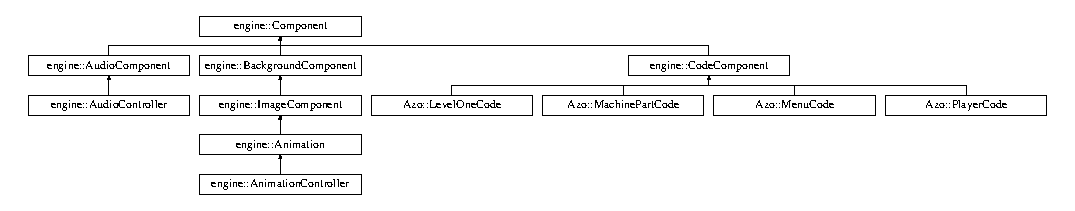
\includegraphics[height=2.393162cm]{classengine_1_1_component}
\end{center}
\end{figure}
\subsection*{Public Member Functions}
\begin{DoxyCompactItemize}
\item 
\hyperlink{classengine_1_1_component_a8775db6d1a2c1afc2e77cd3c8f39da6f}{Component} ()
\begin{DoxyCompactList}\small\item\em Default constructor for the component. \end{DoxyCompactList}\item 
\hyperlink{classengine_1_1_component_aa724dee82c2f103886b0663e8fd085a0}{Component} (\hyperlink{classengine_1_1_game_object}{Game\+Object} \&\hyperlink{classengine_1_1_component_ad4a4865ca4df98ebea34d04a4ec5ad07}{game\+Object})
\begin{DoxyCompactList}\small\item\em Constructor for the component. \end{DoxyCompactList}\item 
virtual void \hyperlink{classengine_1_1_component_aa0bf4fb5f4bc0de25d3f7beef3a3ca45}{init} ()
\begin{DoxyCompactList}\small\item\em inherits function that initialize the game components \end{DoxyCompactList}\item 
virtual void \hyperlink{classengine_1_1_component_a3e47775d51e78914bdfebba123354849}{shutdown} ()
\begin{DoxyCompactList}\small\item\em inherits function that disable the game components \end{DoxyCompactList}\item 
virtual void \hyperlink{classengine_1_1_component_a3d20060d4af0bf0dd0c833994581bdfa}{draw} ()
\begin{DoxyCompactList}\small\item\em inherits function that draw game objects. \end{DoxyCompactList}\item 
virtual void \hyperlink{classengine_1_1_component_a21fd10ef0e28e9c930ccbffa943486aa}{update\+Code} ()
\begin{DoxyCompactList}\small\item\em inherits function that update the game code. \end{DoxyCompactList}\item 
virtual void \hyperlink{classengine_1_1_component_ae4e0b2575af124b63c7c5c15765c3add}{enable\+Component} ()
\begin{DoxyCompactList}\small\item\em enable components. \end{DoxyCompactList}\item 
virtual void \hyperlink{classengine_1_1_component_a9c42e55639174abeda044285a8b1db4b}{disable\+Component} ()
\begin{DoxyCompactList}\small\item\em disable components. \end{DoxyCompactList}\item 
bool \hyperlink{classengine_1_1_component_aa22ebfe0829ab3f1609fd139ddd0ff54}{is\+Enabled} ()
\begin{DoxyCompactList}\small\item\em test if component is enable. \end{DoxyCompactList}\item 
virtual std\+::string \hyperlink{classengine_1_1_component_a4341ed3c744b160590908bea151b6ca7}{get\+Class\+Name} ()
\begin{DoxyCompactList}\small\item\em access the name of the class. \end{DoxyCompactList}\end{DoxyCompactItemize}
\subsection*{Protected Attributes}
\begin{DoxyCompactItemize}
\item 
\hyperlink{classengine_1_1_game_object}{Game\+Object} $\ast$ \hyperlink{classengine_1_1_component_ad4a4865ca4df98ebea34d04a4ec5ad07}{game\+Object}
\item 
\hyperlink{namespaceengine_aa1fd544a3408d033764aa448ec42c912}{State} \hyperlink{classengine_1_1_component_acd64e7e69db92dbdafe70d208dc1c85e}{component\+State} = State\+::\+E\+N\+A\+B\+L\+ED
\end{DoxyCompactItemize}


\subsection{Detailed Description}
A \hyperlink{classengine_1_1_component}{Component} class. 

Generic \hyperlink{classengine_1_1_component}{Component} class. It\textquotesingle{}s how the engine\textquotesingle{}ll see all components that will try to use it. 

Definition at line 43 of file component.\+hpp.



\subsection{Constructor \& Destructor Documentation}
\index{engine\+::\+Component@{engine\+::\+Component}!Component@{Component}}
\index{Component@{Component}!engine\+::\+Component@{engine\+::\+Component}}
\subsubsection[{\texorpdfstring{Component()}{Component()}}]{\setlength{\rightskip}{0pt plus 5cm}Component\+::\+Component (
\begin{DoxyParamCaption}
{}
\end{DoxyParamCaption}
)}\hypertarget{classengine_1_1_component_a8775db6d1a2c1afc2e77cd3c8f39da6f}{}\label{classengine_1_1_component_a8775db6d1a2c1afc2e77cd3c8f39da6f}


Default constructor for the component. 

\begin{DoxyReturn}{Returns}
\char`\"{}void\char`\"{}. 
\end{DoxyReturn}


Definition at line 22 of file component.\+cpp.

\index{engine\+::\+Component@{engine\+::\+Component}!Component@{Component}}
\index{Component@{Component}!engine\+::\+Component@{engine\+::\+Component}}
\subsubsection[{\texorpdfstring{Component(\+Game\+Object \&game\+Object)}{Component(GameObject &gameObject)}}]{\setlength{\rightskip}{0pt plus 5cm}Component\+::\+Component (
\begin{DoxyParamCaption}
\item[{{\bf Game\+Object} \&}]{game\+Object}
\end{DoxyParamCaption}
)}\hypertarget{classengine_1_1_component_aa724dee82c2f103886b0663e8fd085a0}{}\label{classengine_1_1_component_aa724dee82c2f103886b0663e8fd085a0}


Constructor for the component. 


\begin{DoxyParams}{Parameters}
{\em game} & object to the component.\\
\hline
\end{DoxyParams}
\begin{DoxyReturn}{Returns}
\char`\"{}void\char`\"{}. 
\end{DoxyReturn}


Definition at line 31 of file component.\+cpp.



\subsection{Member Function Documentation}
\index{engine\+::\+Component@{engine\+::\+Component}!disable\+Component@{disable\+Component}}
\index{disable\+Component@{disable\+Component}!engine\+::\+Component@{engine\+::\+Component}}
\subsubsection[{\texorpdfstring{disable\+Component()}{disableComponent()}}]{\setlength{\rightskip}{0pt plus 5cm}void Component\+::disable\+Component (
\begin{DoxyParamCaption}
{}
\end{DoxyParamCaption}
)\hspace{0.3cm}{\ttfamily [virtual]}}\hypertarget{classengine_1_1_component_a9c42e55639174abeda044285a8b1db4b}{}\label{classengine_1_1_component_a9c42e55639174abeda044285a8b1db4b}


disable components. 

set the game object components state to disabled.

\begin{DoxyReturn}{Returns}
\char`\"{}void\char`\"{}. 
\end{DoxyReturn}


Reimplemented in \hyperlink{classengine_1_1_animation_aed6b685cec9e13063f171ce6bd49b9d7}{engine\+::\+Animation}.



Definition at line 90 of file component.\+cpp.

\index{engine\+::\+Component@{engine\+::\+Component}!draw@{draw}}
\index{draw@{draw}!engine\+::\+Component@{engine\+::\+Component}}
\subsubsection[{\texorpdfstring{draw()}{draw()}}]{\setlength{\rightskip}{0pt plus 5cm}void Component\+::draw (
\begin{DoxyParamCaption}
{}
\end{DoxyParamCaption}
)\hspace{0.3cm}{\ttfamily [virtual]}}\hypertarget{classengine_1_1_component_a3d20060d4af0bf0dd0c833994581bdfa}{}\label{classengine_1_1_component_a3d20060d4af0bf0dd0c833994581bdfa}


inherits function that draw game objects. 

draws all the enabled game objects.

\begin{DoxyReturn}{Returns}
\char`\"{}void\char`\"{}. 
\end{DoxyReturn}


Reimplemented in \hyperlink{classengine_1_1_animation_a5bc1f5aaee0372f573d4537dab43a162}{engine\+::\+Animation}, \hyperlink{classengine_1_1_animation_controller_a906d2adadfd5eeb2dc6edff3e2f15c45}{engine\+::\+Animation\+Controller}, \hyperlink{classengine_1_1_background_component_a7b3c366c4b917888bde48917d83994be}{engine\+::\+Background\+Component}, and \hyperlink{classengine_1_1_image_component_a2be1a46da22f0f2280f7748c49fa6276}{engine\+::\+Image\+Component}.



Definition at line 61 of file component.\+cpp.

\index{engine\+::\+Component@{engine\+::\+Component}!enable\+Component@{enable\+Component}}
\index{enable\+Component@{enable\+Component}!engine\+::\+Component@{engine\+::\+Component}}
\subsubsection[{\texorpdfstring{enable\+Component()}{enableComponent()}}]{\setlength{\rightskip}{0pt plus 5cm}void Component\+::enable\+Component (
\begin{DoxyParamCaption}
{}
\end{DoxyParamCaption}
)\hspace{0.3cm}{\ttfamily [virtual]}}\hypertarget{classengine_1_1_component_ae4e0b2575af124b63c7c5c15765c3add}{}\label{classengine_1_1_component_ae4e0b2575af124b63c7c5c15765c3add}


enable components. 

set the game object components state to enabled.

\begin{DoxyReturn}{Returns}
\char`\"{}void\char`\"{}. 
\end{DoxyReturn}


Definition at line 79 of file component.\+cpp.

\index{engine\+::\+Component@{engine\+::\+Component}!get\+Class\+Name@{get\+Class\+Name}}
\index{get\+Class\+Name@{get\+Class\+Name}!engine\+::\+Component@{engine\+::\+Component}}
\subsubsection[{\texorpdfstring{get\+Class\+Name()}{getClassName()}}]{\setlength{\rightskip}{0pt plus 5cm}virtual std\+::string engine\+::\+Component\+::get\+Class\+Name (
\begin{DoxyParamCaption}
{}
\end{DoxyParamCaption}
)\hspace{0.3cm}{\ttfamily [inline]}, {\ttfamily [virtual]}}\hypertarget{classengine_1_1_component_a4341ed3c744b160590908bea151b6ca7}{}\label{classengine_1_1_component_a4341ed3c744b160590908bea151b6ca7}


access the name of the class. 

Used to get the private attribute class\+Name.

\begin{DoxyReturn}{Returns}
string that contains the scene name. 
\end{DoxyReturn}


Reimplemented in \hyperlink{classengine_1_1_animation_a6d7f93578e25311f51f2b3c737f885b2}{engine\+::\+Animation}, \hyperlink{classengine_1_1_animation_controller_a227866340161b386c3e39503a15e03cc}{engine\+::\+Animation\+Controller}, \hyperlink{classengine_1_1_background_component_ad3283bbe6ab2d5c170ca67d2180c9fe2}{engine\+::\+Background\+Component}, and \hyperlink{classengine_1_1_image_component_ac18bc924683d4d389b6706abd0afab20}{engine\+::\+Image\+Component}.



Definition at line 66 of file component.\+hpp.

\index{engine\+::\+Component@{engine\+::\+Component}!init@{init}}
\index{init@{init}!engine\+::\+Component@{engine\+::\+Component}}
\subsubsection[{\texorpdfstring{init()}{init()}}]{\setlength{\rightskip}{0pt plus 5cm}void Component\+::init (
\begin{DoxyParamCaption}
{}
\end{DoxyParamCaption}
)\hspace{0.3cm}{\ttfamily [virtual]}}\hypertarget{classengine_1_1_component_aa0bf4fb5f4bc0de25d3f7beef3a3ca45}{}\label{classengine_1_1_component_aa0bf4fb5f4bc0de25d3f7beef3a3ca45}


inherits function that initialize the game components 

Set all game components to enable

\begin{DoxyReturn}{Returns}
\char`\"{}void\char`\"{}. 
\end{DoxyReturn}


Reimplemented in \hyperlink{classengine_1_1_audio_component_a61f7e9f09253a0619ed979276267150c}{engine\+::\+Audio\+Component}, \hyperlink{classengine_1_1_animation_controller_ae40c2032604f044293d50c27da416f01}{engine\+::\+Animation\+Controller}, \hyperlink{classengine_1_1_audio_controller_a34af3c91cadbf4a97eafdd3e311671c9}{engine\+::\+Audio\+Controller}, \hyperlink{classengine_1_1_background_component_a88a96b265f85934474d23d37cb2e6413}{engine\+::\+Background\+Component}, \hyperlink{classengine_1_1_image_component_a4e5def28ca4647b29a4fe9bda78f9e57}{engine\+::\+Image\+Component}, and \hyperlink{classengine_1_1_code_component_a710d9f79114c7b055aaa94fae179ae55}{engine\+::\+Code\+Component}.



Definition at line 43 of file component.\+cpp.

\index{engine\+::\+Component@{engine\+::\+Component}!is\+Enabled@{is\+Enabled}}
\index{is\+Enabled@{is\+Enabled}!engine\+::\+Component@{engine\+::\+Component}}
\subsubsection[{\texorpdfstring{is\+Enabled()}{isEnabled()}}]{\setlength{\rightskip}{0pt plus 5cm}bool Component\+::is\+Enabled (
\begin{DoxyParamCaption}
{}
\end{DoxyParamCaption}
)}\hypertarget{classengine_1_1_component_aa22ebfe0829ab3f1609fd139ddd0ff54}{}\label{classengine_1_1_component_aa22ebfe0829ab3f1609fd139ddd0ff54}


test if component is enable. 

allows see if component is enable or disable.

\begin{DoxyReturn}{Returns}
bool that response if component is enabled. 
\end{DoxyReturn}


Definition at line 101 of file component.\+cpp.

\index{engine\+::\+Component@{engine\+::\+Component}!shutdown@{shutdown}}
\index{shutdown@{shutdown}!engine\+::\+Component@{engine\+::\+Component}}
\subsubsection[{\texorpdfstring{shutdown()}{shutdown()}}]{\setlength{\rightskip}{0pt plus 5cm}void Component\+::shutdown (
\begin{DoxyParamCaption}
{}
\end{DoxyParamCaption}
)\hspace{0.3cm}{\ttfamily [virtual]}}\hypertarget{classengine_1_1_component_a3e47775d51e78914bdfebba123354849}{}\label{classengine_1_1_component_a3e47775d51e78914bdfebba123354849}


inherits function that disable the game components 

free the component pointers

\begin{DoxyReturn}{Returns}
\char`\"{}void\char`\"{}. 
\end{DoxyReturn}


Reimplemented in \hyperlink{classengine_1_1_animation_a219053e2c5bc9179fa355f14cf9bf032}{engine\+::\+Animation}, \hyperlink{classengine_1_1_audio_component_acb42c8fa38793ff0fe6c0652bbb9eac9}{engine\+::\+Audio\+Component}, \hyperlink{class_azo_1_1_player_code_aea1004e3e9f7c7c58d69f428dd0b5b6f}{Azo\+::\+Player\+Code}, \hyperlink{classengine_1_1_animation_controller_a63ed3b30c0ea1fba109e6bed452c21ce}{engine\+::\+Animation\+Controller}, \hyperlink{class_azo_1_1_level_one_code_af66d92f836d8a6c0f72d718d05db63a5}{Azo\+::\+Level\+One\+Code}, \hyperlink{classengine_1_1_audio_controller_aaeb8eaadaa523db5e3608f019fe1bf8e}{engine\+::\+Audio\+Controller}, \hyperlink{classengine_1_1_background_component_a88da6fd205007306776b1ff186b29668}{engine\+::\+Background\+Component}, \hyperlink{classengine_1_1_code_component_af76ba17f9f87216418081d1e2c7c3a22}{engine\+::\+Code\+Component}, and \hyperlink{class_azo_1_1_machine_part_code_aea9e8e5ccc20e0ac975277104b29d0bf}{Azo\+::\+Machine\+Part\+Code}.



Definition at line 52 of file component.\+cpp.

\index{engine\+::\+Component@{engine\+::\+Component}!update\+Code@{update\+Code}}
\index{update\+Code@{update\+Code}!engine\+::\+Component@{engine\+::\+Component}}
\subsubsection[{\texorpdfstring{update\+Code()}{updateCode()}}]{\setlength{\rightskip}{0pt plus 5cm}void Component\+::update\+Code (
\begin{DoxyParamCaption}
{}
\end{DoxyParamCaption}
)\hspace{0.3cm}{\ttfamily [virtual]}}\hypertarget{classengine_1_1_component_a21fd10ef0e28e9c930ccbffa943486aa}{}\label{classengine_1_1_component_a21fd10ef0e28e9c930ccbffa943486aa}


inherits function that update the game code. 

update all the enabled game objects.

\begin{DoxyReturn}{Returns}
\char`\"{}void\char`\"{}. 
\end{DoxyReturn}


Reimplemented in \hyperlink{classengine_1_1_audio_component_aa35e7f57c104c2281680bb13764e4ef0}{engine\+::\+Audio\+Component}, \hyperlink{classengine_1_1_audio_controller_acbbf0bd451c181fb1e3dc26e7c4be27d}{engine\+::\+Audio\+Controller}, and \hyperlink{classengine_1_1_code_component_a78363275025956ccdbfa11fd42f8ae96}{engine\+::\+Code\+Component}.



Definition at line 70 of file component.\+cpp.



\subsection{Member Data Documentation}
\index{engine\+::\+Component@{engine\+::\+Component}!component\+State@{component\+State}}
\index{component\+State@{component\+State}!engine\+::\+Component@{engine\+::\+Component}}
\subsubsection[{\texorpdfstring{component\+State}{componentState}}]{\setlength{\rightskip}{0pt plus 5cm}{\bf State} engine\+::\+Component\+::component\+State = State\+::\+E\+N\+A\+B\+L\+ED\hspace{0.3cm}{\ttfamily [protected]}}\hypertarget{classengine_1_1_component_acd64e7e69db92dbdafe70d208dc1c85e}{}\label{classengine_1_1_component_acd64e7e69db92dbdafe70d208dc1c85e}


Definition at line 47 of file component.\+hpp.

\index{engine\+::\+Component@{engine\+::\+Component}!game\+Object@{game\+Object}}
\index{game\+Object@{game\+Object}!engine\+::\+Component@{engine\+::\+Component}}
\subsubsection[{\texorpdfstring{game\+Object}{gameObject}}]{\setlength{\rightskip}{0pt plus 5cm}{\bf Game\+Object}$\ast$ engine\+::\+Component\+::game\+Object\hspace{0.3cm}{\ttfamily [protected]}}\hypertarget{classengine_1_1_component_ad4a4865ca4df98ebea34d04a4ec5ad07}{}\label{classengine_1_1_component_ad4a4865ca4df98ebea34d04a4ec5ad07}


Definition at line 46 of file component.\+hpp.



The documentation for this class was generated from the following files\+:\begin{DoxyCompactItemize}
\item 
engine/include/\hyperlink{component_8hpp}{component.\+hpp}\item 
engine/src/\hyperlink{component_8cpp}{component.\+cpp}\end{DoxyCompactItemize}

\hypertarget{classengine_1_1_game}{}\section{engine\+:\+:Game Class Reference}
\label{classengine_1_1_game}\index{engine\+::\+Game@{engine\+::\+Game}}


A \hyperlink{classengine_1_1_game}{Game} class.  




{\ttfamily \#include $<$game.\+hpp$>$}

\subsection*{Public Member Functions}
\begin{DoxyCompactItemize}
\item 
\hyperlink{classengine_1_1_game_ad59df6562a58a614fda24622d3715b65}{Game} ()
\begin{DoxyCompactList}\small\item\em Default constructor for the \hyperlink{classengine_1_1_game}{Game} component. \end{DoxyCompactList}\item 
void \hyperlink{classengine_1_1_game_a1ab78f5ed0d5ea879157357cf2fb2afa}{run} ()
\begin{DoxyCompactList}\small\item\em Main \hyperlink{classengine_1_1_game}{Game} Loop and \hyperlink{classengine_1_1_s_d_l}{S\+DL} Initiators. \end{DoxyCompactList}\item 
bool \hyperlink{classengine_1_1_game_a0c4045649cdb6a1e1a804b6f1c136ec3}{add\+Scene} (\hyperlink{classengine_1_1_scene}{engine\+::\+Scene} \&scene)
\begin{DoxyCompactList}\small\item\em add scenes to the game. \end{DoxyCompactList}\item 
void \hyperlink{classengine_1_1_game_ae3e212e771960fda160fd298306460c8}{restart\+Scene} (std\+::string scene\+Name)
\begin{DoxyCompactList}\small\item\em Restart game scene. \end{DoxyCompactList}\item 
void \hyperlink{classengine_1_1_game_a8f6fd890cc6a5c4e4fc8fa5b325d0ca3}{set\+Attributes} (std\+::string game\+Name, int window\+Width, int window\+Height, int frame\+Rate)
\begin{DoxyCompactList}\small\item\em set the game attributtes to \hyperlink{classengine_1_1_s_d_l}{S\+DL} instance. \end{DoxyCompactList}\item 
\hyperlink{classengine_1_1_timer}{Timer} \& \hyperlink{classengine_1_1_game_af3b784dd57665c8b8cfa8d17e70fff9a}{get\+Timer} ()
\begin{DoxyCompactList}\small\item\em access the \hyperlink{classengine_1_1_timer}{Timer}. \end{DoxyCompactList}\item 
\hyperlink{classengine_1_1_assets_manager}{Assets\+Manager} \& \hyperlink{classengine_1_1_game_ae47c2387cf5bd6881161ae6f556fe385}{get\+Assets\+Manager} ()
\begin{DoxyCompactList}\small\item\em access the assets manager. \end{DoxyCompactList}\item 
void \hyperlink{classengine_1_1_game_a7150904ff2536b8553b4a152a724c67c}{change\+Scene} (std\+::string scene\+Name)
\begin{DoxyCompactList}\small\item\em change the game scene. \end{DoxyCompactList}\end{DoxyCompactItemize}
\subsection*{Public Attributes}
\begin{DoxyCompactItemize}
\item 
\hyperlink{classengine_1_1_s_d_l}{S\+DL} \hyperlink{classengine_1_1_game_ab4a295f7b30b191183d5411f5fa5d66b}{sdl\+Elements}
\item 
\hyperlink{classengine_1_1_input_manager}{Input\+Manager} \hyperlink{classengine_1_1_game_ab9e84515e30301e673fa693c676f0c63}{input\+Manager}
\item 
\hyperlink{namespaceengine_af41e517ae74e4a8447ff80a2abcaf8dd}{Game\+State} \hyperlink{classengine_1_1_game_a6e5b7bd8569cf22309b9f934ba426eae}{game\+State}
\end{DoxyCompactItemize}
\subsection*{Static Public Attributes}
\begin{DoxyCompactItemize}
\item 
static \hyperlink{classengine_1_1_game}{Game} \hyperlink{classengine_1_1_game_aed34cffcaed0e8027c11d68b1d42258b}{instance}
\end{DoxyCompactItemize}


\subsection{Detailed Description}
A \hyperlink{classengine_1_1_game}{Game} class. 

Generic \hyperlink{classengine_1_1_game}{Game} class. It\textquotesingle{}s how the engine\textquotesingle{}ll see all games that will try to use it. 

Definition at line 46 of file game.\+hpp.



\subsection{Constructor \& Destructor Documentation}
\index{engine\+::\+Game@{engine\+::\+Game}!Game@{Game}}
\index{Game@{Game}!engine\+::\+Game@{engine\+::\+Game}}
\subsubsection[{\texorpdfstring{Game()}{Game()}}]{\setlength{\rightskip}{0pt plus 5cm}Game\+::\+Game (
\begin{DoxyParamCaption}
{}
\end{DoxyParamCaption}
)}\hypertarget{classengine_1_1_game_ad59df6562a58a614fda24622d3715b65}{}\label{classengine_1_1_game_ad59df6562a58a614fda24622d3715b65}


Default constructor for the \hyperlink{classengine_1_1_game}{Game} component. 

\begin{DoxyReturn}{Returns}
\char`\"{}void\char`\"{}. 
\end{DoxyReturn}


Definition at line 27 of file game.\+cpp.



\subsection{Member Function Documentation}
\index{engine\+::\+Game@{engine\+::\+Game}!add\+Scene@{add\+Scene}}
\index{add\+Scene@{add\+Scene}!engine\+::\+Game@{engine\+::\+Game}}
\subsubsection[{\texorpdfstring{add\+Scene(engine\+::\+Scene \&scene)}{addScene(engine::Scene &scene)}}]{\setlength{\rightskip}{0pt plus 5cm}bool Game\+::add\+Scene (
\begin{DoxyParamCaption}
\item[{{\bf engine\+::\+Scene} \&}]{scene}
\end{DoxyParamCaption}
)}\hypertarget{classengine_1_1_game_a0c4045649cdb6a1e1a804b6f1c136ec3}{}\label{classengine_1_1_game_a0c4045649cdb6a1e1a804b6f1c136ec3}


add scenes to the game. 

Used to add a \hyperlink{classengine_1_1_scene}{Scene} to map that have all \hyperlink{classengine_1_1_game}{Game}\textquotesingle{}s Scenes.


\begin{DoxyParams}{Parameters}
{\em \hyperlink{classengine_1_1_scene}{Scene}} & that represent a game stage.\\
\hline
\end{DoxyParams}
\begin{DoxyReturn}{Returns}
a bool that indicates the add scene success. 
\end{DoxyReturn}


Definition at line 110 of file game.\+cpp.

\index{engine\+::\+Game@{engine\+::\+Game}!change\+Scene@{change\+Scene}}
\index{change\+Scene@{change\+Scene}!engine\+::\+Game@{engine\+::\+Game}}
\subsubsection[{\texorpdfstring{change\+Scene(std\+::string scene\+Name)}{changeScene(std::string sceneName)}}]{\setlength{\rightskip}{0pt plus 5cm}void Game\+::change\+Scene (
\begin{DoxyParamCaption}
\item[{std\+::string}]{scene\+Name}
\end{DoxyParamCaption}
)}\hypertarget{classengine_1_1_game_a7150904ff2536b8553b4a152a724c67c}{}\label{classengine_1_1_game_a7150904ff2536b8553b4a152a724c67c}


change the game scene. 

Perform the necessary checks and prepare the structure to switch Scenes.


\begin{DoxyParams}{Parameters}
{\em scene\+Name} & string that has the scene name\\
\hline
\end{DoxyParams}
\begin{DoxyReturn}{Returns}
\char`\"{}void\char`\"{}. 
\end{DoxyReturn}


Definition at line 147 of file game.\+cpp.

\index{engine\+::\+Game@{engine\+::\+Game}!get\+Assets\+Manager@{get\+Assets\+Manager}}
\index{get\+Assets\+Manager@{get\+Assets\+Manager}!engine\+::\+Game@{engine\+::\+Game}}
\subsubsection[{\texorpdfstring{get\+Assets\+Manager()}{getAssetsManager()}}]{\setlength{\rightskip}{0pt plus 5cm}{\bf Assets\+Manager}\& engine\+::\+Game\+::get\+Assets\+Manager (
\begin{DoxyParamCaption}
{}
\end{DoxyParamCaption}
)\hspace{0.3cm}{\ttfamily [inline]}}\hypertarget{classengine_1_1_game_ae47c2387cf5bd6881161ae6f556fe385}{}\label{classengine_1_1_game_ae47c2387cf5bd6881161ae6f556fe385}


access the assets manager. 

Used to get the private attribute \hyperlink{classengine_1_1_assets_manager}{Assets\+Manager}.

\begin{DoxyReturn}{Returns}
the game assets manager. 
\end{DoxyReturn}


Definition at line 91 of file game.\+hpp.

\index{engine\+::\+Game@{engine\+::\+Game}!get\+Timer@{get\+Timer}}
\index{get\+Timer@{get\+Timer}!engine\+::\+Game@{engine\+::\+Game}}
\subsubsection[{\texorpdfstring{get\+Timer()}{getTimer()}}]{\setlength{\rightskip}{0pt plus 5cm}{\bf Timer}\& engine\+::\+Game\+::get\+Timer (
\begin{DoxyParamCaption}
{}
\end{DoxyParamCaption}
)\hspace{0.3cm}{\ttfamily [inline]}}\hypertarget{classengine_1_1_game_af3b784dd57665c8b8cfa8d17e70fff9a}{}\label{classengine_1_1_game_af3b784dd57665c8b8cfa8d17e70fff9a}


access the \hyperlink{classengine_1_1_timer}{Timer}. 

Used to get the private attribute \hyperlink{classengine_1_1_timer}{Timer}.

\begin{DoxyReturn}{Returns}
the game timer. 
\end{DoxyReturn}


Definition at line 80 of file game.\+hpp.

\index{engine\+::\+Game@{engine\+::\+Game}!restart\+Scene@{restart\+Scene}}
\index{restart\+Scene@{restart\+Scene}!engine\+::\+Game@{engine\+::\+Game}}
\subsubsection[{\texorpdfstring{restart\+Scene(std\+::string scene\+Name)}{restartScene(std::string sceneName)}}]{\setlength{\rightskip}{0pt plus 5cm}void Game\+::restart\+Scene (
\begin{DoxyParamCaption}
\item[{std\+::string}]{scene\+Name}
\end{DoxyParamCaption}
)}\hypertarget{classengine_1_1_game_ae3e212e771960fda160fd298306460c8}{}\label{classengine_1_1_game_ae3e212e771960fda160fd298306460c8}


Restart game scene. 

Load the scene. Used every time a scene needs to be reseted.


\begin{DoxyParams}{Parameters}
{\em scene\+Name} & string that has the scene name.\\
\hline
\end{DoxyParams}
\begin{DoxyReturn}{Returns}
\char`\"{}void\char`\"{}. 
\end{DoxyReturn}


Definition at line 132 of file game.\+cpp.

\index{engine\+::\+Game@{engine\+::\+Game}!run@{run}}
\index{run@{run}!engine\+::\+Game@{engine\+::\+Game}}
\subsubsection[{\texorpdfstring{run()}{run()}}]{\setlength{\rightskip}{0pt plus 5cm}void Game\+::run (
\begin{DoxyParamCaption}
{}
\end{DoxyParamCaption}
)}\hypertarget{classengine_1_1_game_a1ab78f5ed0d5ea879157357cf2fb2afa}{}\label{classengine_1_1_game_a1ab78f5ed0d5ea879157357cf2fb2afa}


Main \hyperlink{classengine_1_1_game}{Game} Loop and \hyperlink{classengine_1_1_s_d_l}{S\+DL} Initiators. 

Run all the game.

\begin{DoxyReturn}{Returns}
\char`\"{}void\char`\"{}. 
\end{DoxyReturn}
If the time that has passed until now was faster than the frame\textquotesingle{}s time, is needed wait the time necessary to complete a frame\textquotesingle{}s time.

Definition at line 41 of file game.\+cpp.

\index{engine\+::\+Game@{engine\+::\+Game}!set\+Attributes@{set\+Attributes}}
\index{set\+Attributes@{set\+Attributes}!engine\+::\+Game@{engine\+::\+Game}}
\subsubsection[{\texorpdfstring{set\+Attributes(std\+::string game\+Name, int window\+Width, int window\+Height, int frame\+Rate)}{setAttributes(std::string gameName, int windowWidth, int windowHeight, int frameRate)}}]{\setlength{\rightskip}{0pt plus 5cm}void Game\+::set\+Attributes (
\begin{DoxyParamCaption}
\item[{std\+::string}]{game\+Name, }
\item[{int}]{window\+Width, }
\item[{int}]{window\+Height, }
\item[{int}]{frame\+Rate}
\end{DoxyParamCaption}
)}\hypertarget{classengine_1_1_game_a8f6fd890cc6a5c4e4fc8fa5b325d0ca3}{}\label{classengine_1_1_game_a8f6fd890cc6a5c4e4fc8fa5b325d0ca3}


set the game attributtes to \hyperlink{classengine_1_1_s_d_l}{S\+DL} instance. 

Transfer the game attributes to \hyperlink{classengine_1_1_s_d_l}{S\+DL} instace and set \hyperlink{classengine_1_1_game}{Game}\textquotesingle{}s frame\+Rate.


\begin{DoxyParams}{Parameters}
{\em game\+Name} & string that has the name of the game \\
\hline
{\em window\+Width} & sets the width of the game screen \\
\hline
{\em window\+Height} & sets the height of the game screen \\
\hline
{\em frame\+Rate} & Frames per Second of the \hyperlink{classengine_1_1_game}{Game} (F\+PS).\\
\hline
\end{DoxyParams}
\begin{DoxyReturn}{Returns}
\char`\"{}void\char`\"{}. 
\end{DoxyReturn}


Definition at line 216 of file game.\+cpp.



\subsection{Member Data Documentation}
\index{engine\+::\+Game@{engine\+::\+Game}!game\+State@{game\+State}}
\index{game\+State@{game\+State}!engine\+::\+Game@{engine\+::\+Game}}
\subsubsection[{\texorpdfstring{game\+State}{gameState}}]{\setlength{\rightskip}{0pt plus 5cm}{\bf Game\+State} engine\+::\+Game\+::game\+State}\hypertarget{classengine_1_1_game_a6e5b7bd8569cf22309b9f934ba426eae}{}\label{classengine_1_1_game_a6e5b7bd8569cf22309b9f934ba426eae}


Definition at line 51 of file game.\+hpp.

\index{engine\+::\+Game@{engine\+::\+Game}!input\+Manager@{input\+Manager}}
\index{input\+Manager@{input\+Manager}!engine\+::\+Game@{engine\+::\+Game}}
\subsubsection[{\texorpdfstring{input\+Manager}{inputManager}}]{\setlength{\rightskip}{0pt plus 5cm}{\bf Input\+Manager} engine\+::\+Game\+::input\+Manager}\hypertarget{classengine_1_1_game_ab9e84515e30301e673fa693c676f0c63}{}\label{classengine_1_1_game_ab9e84515e30301e673fa693c676f0c63}


Definition at line 50 of file game.\+hpp.

\index{engine\+::\+Game@{engine\+::\+Game}!instance@{instance}}
\index{instance@{instance}!engine\+::\+Game@{engine\+::\+Game}}
\subsubsection[{\texorpdfstring{instance}{instance}}]{\setlength{\rightskip}{0pt plus 5cm}{\bf Game} Game\+::instance\hspace{0.3cm}{\ttfamily [static]}}\hypertarget{classengine_1_1_game_aed34cffcaed0e8027c11d68b1d42258b}{}\label{classengine_1_1_game_aed34cffcaed0e8027c11d68b1d42258b}


Definition at line 48 of file game.\+hpp.

\index{engine\+::\+Game@{engine\+::\+Game}!sdl\+Elements@{sdl\+Elements}}
\index{sdl\+Elements@{sdl\+Elements}!engine\+::\+Game@{engine\+::\+Game}}
\subsubsection[{\texorpdfstring{sdl\+Elements}{sdlElements}}]{\setlength{\rightskip}{0pt plus 5cm}{\bf S\+DL} engine\+::\+Game\+::sdl\+Elements}\hypertarget{classengine_1_1_game_ab4a295f7b30b191183d5411f5fa5d66b}{}\label{classengine_1_1_game_ab4a295f7b30b191183d5411f5fa5d66b}


Definition at line 49 of file game.\+hpp.



The documentation for this class was generated from the following files\+:\begin{DoxyCompactItemize}
\item 
engine/include/\hyperlink{game_8hpp}{game.\+hpp}\item 
engine/src/\hyperlink{game_8cpp}{game.\+cpp}\end{DoxyCompactItemize}

\hypertarget{classengine_1_1_game_object}{}\section{engine\+:\+:Game\+Object Class Reference}
\label{classengine_1_1_game_object}\index{engine\+::\+Game\+Object@{engine\+::\+Game\+Object}}


A \hyperlink{classengine_1_1_game}{Game} Object class.  




{\ttfamily \#include $<$game\+\_\+object.\+hpp$>$}

Inheritance diagram for engine\+:\+:Game\+Object\+:\begin{figure}[H]
\begin{center}
\leavevmode
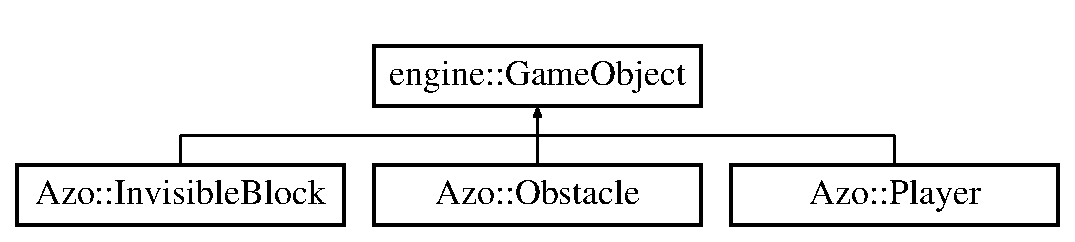
\includegraphics[height=2.000000cm]{classengine_1_1_game_object}
\end{center}
\end{figure}
\subsection*{Public Member Functions}
\begin{DoxyCompactItemize}
\item 
\hyperlink{classengine_1_1_game_object_a0348e3ee2e83d56eafca7a3547f432c4}{Game\+Object} ()
\begin{DoxyCompactList}\small\item\em Default constructor for the \hyperlink{classengine_1_1_game}{Game} Object component. \end{DoxyCompactList}\item 
\hyperlink{classengine_1_1_game_object_a55a9b8b92185ade1c96bac19b10f72ef}{Game\+Object} (std\+::string game\+Object\+Name, std\+::pair$<$ double, double $>$ current\+Position)
\begin{DoxyCompactList}\small\item\em Constructor for the game object. \end{DoxyCompactList}\item 
void \hyperlink{classengine_1_1_game_object_ab0358466033307401a6a0714184503d3}{add\+Component} (\hyperlink{classengine_1_1_component}{Component} \&component)
\begin{DoxyCompactList}\small\item\em add components to the game. \end{DoxyCompactList}\item 
\hyperlink{classengine_1_1_animation_controller}{Animation\+Controller} $\ast$ \hyperlink{classengine_1_1_game_object_a2ed6ce8eadeb37e2eea4f95eaa82b4e4}{get\+Animation\+Controller} (std\+::type\+\_\+index component\+Type)
\begin{DoxyCompactList}\small\item\em retrieve the animation controller. \end{DoxyCompactList}\item 
\hyperlink{classengine_1_1_audio_controller}{Audio\+Controller} $\ast$ \hyperlink{classengine_1_1_game_object_ae14d1f2f05718d3f1e127c81adf6cb36}{get\+Audio\+Controller} (std\+::type\+\_\+index component\+Type)
\begin{DoxyCompactList}\small\item\em retrieve the audio controller. \end{DoxyCompactList}\item 
virtual void \hyperlink{classengine_1_1_game_object_a9b565e5ec63bef28e5c860f724d2de7c}{init} ()
\begin{DoxyCompactList}\small\item\em function that initialize the game objects components. \end{DoxyCompactList}\item 
virtual void \hyperlink{classengine_1_1_game_object_abb64143e72358beb808db22182517802}{draw} ()
\begin{DoxyCompactList}\small\item\em function that draw game objects components. \end{DoxyCompactList}\item 
virtual void \hyperlink{classengine_1_1_game_object_a08d7a48b6eb90f55c8b670b6f98ab393}{shutdown} ()
\begin{DoxyCompactList}\small\item\em inherits function that disable the game components. \end{DoxyCompactList}\item 
virtual void \hyperlink{classengine_1_1_game_object_ac008ad125b3192f0114af78549f6d829}{update\+Code} ()
\begin{DoxyCompactList}\small\item\em function that update the game object code. \end{DoxyCompactList}\item 
virtual std\+::string \hyperlink{classengine_1_1_game_object_ac836deb7933c725ac09b67386ad10239}{get\+Class\+Name} ()
\item 
std\+::pair$<$ double, double $>$ \hyperlink{classengine_1_1_game_object_a615683282d234126169ab8c004c804aa}{calc\+Bottom\+Left} ()
\begin{DoxyCompactList}\small\item\em calculate the bottom left coordinate of a game object. \end{DoxyCompactList}\item 
std\+::pair$<$ double, double $>$ \hyperlink{classengine_1_1_game_object_a804740468e962005e912fb7f5905e5e7}{calc\+Bottom\+Right} ()
\begin{DoxyCompactList}\small\item\em calculate the bottom right coordinate of a game object. \end{DoxyCompactList}\item 
std\+::pair$<$ double, double $>$ \hyperlink{classengine_1_1_game_object_aa1a0d2f7da78692acb1e8e1fde9a7743}{calc\+Top\+Left} ()
\begin{DoxyCompactList}\small\item\em calculate the top left coordinate of a game object. \end{DoxyCompactList}\item 
std\+::pair$<$ double, double $>$ \hyperlink{classengine_1_1_game_object_a86b57828238be71e962132bb28b7e6b7}{calc\+Top\+Right} ()
\begin{DoxyCompactList}\small\item\em calculate the top right coordinate of a game object. \end{DoxyCompactList}\item 
std\+::pair$<$ double, double $>$ \hyperlink{classengine_1_1_game_object_a40e9d29053f3d9e7ccd5f3cadd007f03}{calc\+Right\+Up} ()
\begin{DoxyCompactList}\small\item\em calculate the right up coordinate of a game object. \end{DoxyCompactList}\item 
std\+::pair$<$ double, double $>$ \hyperlink{classengine_1_1_game_object_a85130378e83e5b0d3cba0b98992c4489}{calc\+Right\+Down} ()
\begin{DoxyCompactList}\small\item\em calculate the right down coordinate of a game object. \end{DoxyCompactList}\item 
std\+::pair$<$ double, double $>$ \hyperlink{classengine_1_1_game_object_aabc735b6bccc2106270ee3e09dca21f9}{calc\+Left\+Up} ()
\begin{DoxyCompactList}\small\item\em calculate the left up coordinate of a game object. \end{DoxyCompactList}\item 
std\+::pair$<$ double, double $>$ \hyperlink{classengine_1_1_game_object_aa3215c1412bd15ad3dcd5bbc6e1e3f94}{calc\+Left\+Down} ()
\begin{DoxyCompactList}\small\item\em calculate the left down coordinate of a game object. \end{DoxyCompactList}\end{DoxyCompactItemize}
\subsection*{Public Attributes}
\begin{DoxyCompactItemize}
\item 
std\+::pair$<$ double, double $>$ \hyperlink{classengine_1_1_game_object_a0a4c0a35e88df30bef6e09df9b51e6bd}{m\+Current\+Position}
\item 
std\+::pair$<$ double, double $>$ \hyperlink{classengine_1_1_game_object_a52f18d63910240efdcd7490d81f37dc8}{m\+Size}
\item 
std\+::pair$<$ double, double $>$ \hyperlink{classengine_1_1_game_object_ae1867b69e8bfbf7d9b01a463f2e89e9a}{m\+Center}
\item 
std\+::pair$<$ double, double $>$ \hyperlink{classengine_1_1_game_object_a3d62630e8dc477795f8cc3923747aaba}{m\+Half\+Size}
\item 
std\+::list$<$ \hyperlink{classengine_1_1_game_object}{Game\+Object} $\ast$ $>$ \hyperlink{classengine_1_1_game_object_a407bc88cc30f6432b378da41ba142fae}{m\+Parent\+List}
\item 
std\+::string \hyperlink{classengine_1_1_game_object_af6c682b4912f897b9d798eb5479159bc}{m\+Name}
\item 
\hyperlink{namespaceengine_aae2fae4fa5de0d9b0accc1b59b6c2ff5}{Object\+State} \hyperlink{classengine_1_1_game_object_a14fc4192c3e64ff6c6421add7aeacad8}{m\+Object\+State} = Object\+State\+::\+E\+N\+A\+B\+L\+ED
\end{DoxyCompactItemize}
\subsection*{Protected Attributes}
\begin{DoxyCompactItemize}
\item 
std\+::unordered\+\_\+multimap$<$ std\+::type\+\_\+index, \hyperlink{classengine_1_1_component}{Component} $\ast$ $>$ \hyperlink{classengine_1_1_game_object_a6a2bc7c46e6b3ebce8b8d5a4c152db71}{m\+Component\+Map}
\end{DoxyCompactItemize}


\subsection{Detailed Description}
A \hyperlink{classengine_1_1_game}{Game} Object class. 

Generic \hyperlink{classengine_1_1_game}{Game} Object class. It\textquotesingle{}s how the engine\textquotesingle{}ll see all game objects that will try to use it. 

Definition at line 45 of file game\+\_\+object.\+hpp.



\subsection{Constructor \& Destructor Documentation}
\index{engine\+::\+Game\+Object@{engine\+::\+Game\+Object}!Game\+Object@{Game\+Object}}
\index{Game\+Object@{Game\+Object}!engine\+::\+Game\+Object@{engine\+::\+Game\+Object}}
\subsubsection[{\texorpdfstring{Game\+Object()}{GameObject()}}]{\setlength{\rightskip}{0pt plus 5cm}Game\+Object\+::\+Game\+Object (
\begin{DoxyParamCaption}
{}
\end{DoxyParamCaption}
)}\hypertarget{classengine_1_1_game_object_a0348e3ee2e83d56eafca7a3547f432c4}{}\label{classengine_1_1_game_object_a0348e3ee2e83d56eafca7a3547f432c4}


Default constructor for the \hyperlink{classengine_1_1_game}{Game} Object component. 

\begin{DoxyReturn}{Returns}
\char`\"{}void\char`\"{}. 
\end{DoxyReturn}


Definition at line 24 of file game\+\_\+object.\+cpp.

\index{engine\+::\+Game\+Object@{engine\+::\+Game\+Object}!Game\+Object@{Game\+Object}}
\index{Game\+Object@{Game\+Object}!engine\+::\+Game\+Object@{engine\+::\+Game\+Object}}
\subsubsection[{\texorpdfstring{Game\+Object(std\+::string game\+Object\+Name, std\+::pair$<$ double, double $>$ current\+Position)}{GameObject(std::string gameObjectName, std::pair< double, double > currentPosition)}}]{\setlength{\rightskip}{0pt plus 5cm}Game\+Object\+::\+Game\+Object (
\begin{DoxyParamCaption}
\item[{std\+::string}]{game\+Object\+Name, }
\item[{std\+::pair$<$ double, double $>$}]{current\+Position}
\end{DoxyParamCaption}
)}\hypertarget{classengine_1_1_game_object_a55a9b8b92185ade1c96bac19b10f72ef}{}\label{classengine_1_1_game_object_a55a9b8b92185ade1c96bac19b10f72ef}


Constructor for the game object. 


\begin{DoxyParams}{Parameters}
{\em string} & that has game object name. \\
\hline
{\em pair} & that has the game object current position.\\
\hline
\end{DoxyParams}
\begin{DoxyReturn}{Returns}
\char`\"{}void\char`\"{}. 
\end{DoxyReturn}


Definition at line 39 of file game\+\_\+object.\+cpp.



\subsection{Member Function Documentation}
\index{engine\+::\+Game\+Object@{engine\+::\+Game\+Object}!add\+Component@{add\+Component}}
\index{add\+Component@{add\+Component}!engine\+::\+Game\+Object@{engine\+::\+Game\+Object}}
\subsubsection[{\texorpdfstring{add\+Component(\+Component \&component)}{addComponent(Component &component)}}]{\setlength{\rightskip}{0pt plus 5cm}void Game\+Object\+::add\+Component (
\begin{DoxyParamCaption}
\item[{{\bf Component} \&}]{component}
\end{DoxyParamCaption}
)}\hypertarget{classengine_1_1_game_object_ab0358466033307401a6a0714184503d3}{}\label{classengine_1_1_game_object_ab0358466033307401a6a0714184503d3}


add components to the game. 

set the position and insert the game components.


\begin{DoxyParams}{Parameters}
{\em component} & that is added to the game.\\
\hline
\end{DoxyParams}
\begin{DoxyReturn}{Returns}
\char`\"{}void\char`\"{}. 
\end{DoxyReturn}


Definition at line 53 of file game\+\_\+object.\+cpp.

\index{engine\+::\+Game\+Object@{engine\+::\+Game\+Object}!calc\+Bottom\+Left@{calc\+Bottom\+Left}}
\index{calc\+Bottom\+Left@{calc\+Bottom\+Left}!engine\+::\+Game\+Object@{engine\+::\+Game\+Object}}
\subsubsection[{\texorpdfstring{calc\+Bottom\+Left()}{calcBottomLeft()}}]{\setlength{\rightskip}{0pt plus 5cm}std\+::pair$<$ double, double $>$ Game\+Object\+::calc\+Bottom\+Left (
\begin{DoxyParamCaption}
{}
\end{DoxyParamCaption}
)}\hypertarget{classengine_1_1_game_object_a615683282d234126169ab8c004c804aa}{}\label{classengine_1_1_game_object_a615683282d234126169ab8c004c804aa}


calculate the bottom left coordinate of a game object. 

calculate the bottom left coordinate based on its size and half.

\begin{DoxyReturn}{Returns}
a pair containing the bottom left coordinate of the game object. 
\end{DoxyReturn}


Definition at line 166 of file game\+\_\+object.\+cpp.

\index{engine\+::\+Game\+Object@{engine\+::\+Game\+Object}!calc\+Bottom\+Right@{calc\+Bottom\+Right}}
\index{calc\+Bottom\+Right@{calc\+Bottom\+Right}!engine\+::\+Game\+Object@{engine\+::\+Game\+Object}}
\subsubsection[{\texorpdfstring{calc\+Bottom\+Right()}{calcBottomRight()}}]{\setlength{\rightskip}{0pt plus 5cm}std\+::pair$<$ double, double $>$ Game\+Object\+::calc\+Bottom\+Right (
\begin{DoxyParamCaption}
{}
\end{DoxyParamCaption}
)}\hypertarget{classengine_1_1_game_object_a804740468e962005e912fb7f5905e5e7}{}\label{classengine_1_1_game_object_a804740468e962005e912fb7f5905e5e7}


calculate the bottom right coordinate of a game object. 

calculate the bottom right coordinate based on its size and half.

\begin{DoxyReturn}{Returns}
a pair containing the bottom right coordinate of the game object. 
\end{DoxyReturn}


Definition at line 180 of file game\+\_\+object.\+cpp.

\index{engine\+::\+Game\+Object@{engine\+::\+Game\+Object}!calc\+Left\+Down@{calc\+Left\+Down}}
\index{calc\+Left\+Down@{calc\+Left\+Down}!engine\+::\+Game\+Object@{engine\+::\+Game\+Object}}
\subsubsection[{\texorpdfstring{calc\+Left\+Down()}{calcLeftDown()}}]{\setlength{\rightskip}{0pt plus 5cm}std\+::pair$<$ double, double $>$ Game\+Object\+::calc\+Left\+Down (
\begin{DoxyParamCaption}
{}
\end{DoxyParamCaption}
)}\hypertarget{classengine_1_1_game_object_aa3215c1412bd15ad3dcd5bbc6e1e3f94}{}\label{classengine_1_1_game_object_aa3215c1412bd15ad3dcd5bbc6e1e3f94}


calculate the left down coordinate of a game object. 

calculate the left down coordinate based on bottom left coordinate.

\begin{DoxyReturn}{Returns}
a pair containing the left down coordinate of the game object. 
\end{DoxyReturn}


Definition at line 255 of file game\+\_\+object.\+cpp.

\index{engine\+::\+Game\+Object@{engine\+::\+Game\+Object}!calc\+Left\+Up@{calc\+Left\+Up}}
\index{calc\+Left\+Up@{calc\+Left\+Up}!engine\+::\+Game\+Object@{engine\+::\+Game\+Object}}
\subsubsection[{\texorpdfstring{calc\+Left\+Up()}{calcLeftUp()}}]{\setlength{\rightskip}{0pt plus 5cm}std\+::pair$<$ double, double $>$ Game\+Object\+::calc\+Left\+Up (
\begin{DoxyParamCaption}
{}
\end{DoxyParamCaption}
)}\hypertarget{classengine_1_1_game_object_aabc735b6bccc2106270ee3e09dca21f9}{}\label{classengine_1_1_game_object_aabc735b6bccc2106270ee3e09dca21f9}


calculate the left up coordinate of a game object. 

calculate the left up coordinate based on top left coordinate.

\begin{DoxyReturn}{Returns}
a pair containing the left up coordinate of the game object. 
\end{DoxyReturn}


Definition at line 244 of file game\+\_\+object.\+cpp.

\index{engine\+::\+Game\+Object@{engine\+::\+Game\+Object}!calc\+Right\+Down@{calc\+Right\+Down}}
\index{calc\+Right\+Down@{calc\+Right\+Down}!engine\+::\+Game\+Object@{engine\+::\+Game\+Object}}
\subsubsection[{\texorpdfstring{calc\+Right\+Down()}{calcRightDown()}}]{\setlength{\rightskip}{0pt plus 5cm}std\+::pair$<$ double, double $>$ Game\+Object\+::calc\+Right\+Down (
\begin{DoxyParamCaption}
{}
\end{DoxyParamCaption}
)}\hypertarget{classengine_1_1_game_object_a85130378e83e5b0d3cba0b98992c4489}{}\label{classengine_1_1_game_object_a85130378e83e5b0d3cba0b98992c4489}


calculate the right down coordinate of a game object. 

calculate the right down coordinate based on bottom right coordinate.

\begin{DoxyReturn}{Returns}
a pair containing the right down coordinate of the game object. 
\end{DoxyReturn}


Definition at line 233 of file game\+\_\+object.\+cpp.

\index{engine\+::\+Game\+Object@{engine\+::\+Game\+Object}!calc\+Right\+Up@{calc\+Right\+Up}}
\index{calc\+Right\+Up@{calc\+Right\+Up}!engine\+::\+Game\+Object@{engine\+::\+Game\+Object}}
\subsubsection[{\texorpdfstring{calc\+Right\+Up()}{calcRightUp()}}]{\setlength{\rightskip}{0pt plus 5cm}std\+::pair$<$ double, double $>$ Game\+Object\+::calc\+Right\+Up (
\begin{DoxyParamCaption}
{}
\end{DoxyParamCaption}
)}\hypertarget{classengine_1_1_game_object_a40e9d29053f3d9e7ccd5f3cadd007f03}{}\label{classengine_1_1_game_object_a40e9d29053f3d9e7ccd5f3cadd007f03}


calculate the right up coordinate of a game object. 

calculate the right up coordinate based on top right coordinate.

\begin{DoxyReturn}{Returns}
a pair containing the right up coordinate of the game object. 
\end{DoxyReturn}


Definition at line 222 of file game\+\_\+object.\+cpp.

\index{engine\+::\+Game\+Object@{engine\+::\+Game\+Object}!calc\+Top\+Left@{calc\+Top\+Left}}
\index{calc\+Top\+Left@{calc\+Top\+Left}!engine\+::\+Game\+Object@{engine\+::\+Game\+Object}}
\subsubsection[{\texorpdfstring{calc\+Top\+Left()}{calcTopLeft()}}]{\setlength{\rightskip}{0pt plus 5cm}std\+::pair$<$ double, double $>$ Game\+Object\+::calc\+Top\+Left (
\begin{DoxyParamCaption}
{}
\end{DoxyParamCaption}
)}\hypertarget{classengine_1_1_game_object_aa1a0d2f7da78692acb1e8e1fde9a7743}{}\label{classengine_1_1_game_object_aa1a0d2f7da78692acb1e8e1fde9a7743}


calculate the top left coordinate of a game object. 

calculate the top left coordinate based on its size and half.

\begin{DoxyReturn}{Returns}
a pair containing the top left coordinate of the game object. 
\end{DoxyReturn}


Definition at line 194 of file game\+\_\+object.\+cpp.

\index{engine\+::\+Game\+Object@{engine\+::\+Game\+Object}!calc\+Top\+Right@{calc\+Top\+Right}}
\index{calc\+Top\+Right@{calc\+Top\+Right}!engine\+::\+Game\+Object@{engine\+::\+Game\+Object}}
\subsubsection[{\texorpdfstring{calc\+Top\+Right()}{calcTopRight()}}]{\setlength{\rightskip}{0pt plus 5cm}std\+::pair$<$ double, double $>$ Game\+Object\+::calc\+Top\+Right (
\begin{DoxyParamCaption}
{}
\end{DoxyParamCaption}
)}\hypertarget{classengine_1_1_game_object_a86b57828238be71e962132bb28b7e6b7}{}\label{classengine_1_1_game_object_a86b57828238be71e962132bb28b7e6b7}


calculate the top right coordinate of a game object. 

calculate the top right coordinate based on its size and half.

\begin{DoxyReturn}{Returns}
a pair containing the top right coordinate of the game object. 
\end{DoxyReturn}


Definition at line 208 of file game\+\_\+object.\+cpp.

\index{engine\+::\+Game\+Object@{engine\+::\+Game\+Object}!draw@{draw}}
\index{draw@{draw}!engine\+::\+Game\+Object@{engine\+::\+Game\+Object}}
\subsubsection[{\texorpdfstring{draw()}{draw()}}]{\setlength{\rightskip}{0pt plus 5cm}void Game\+Object\+::draw (
\begin{DoxyParamCaption}
{}
\end{DoxyParamCaption}
)\hspace{0.3cm}{\ttfamily [virtual]}}\hypertarget{classengine_1_1_game_object_abb64143e72358beb808db22182517802}{}\label{classengine_1_1_game_object_abb64143e72358beb808db22182517802}


function that draw game objects components. 

draws all the enabled game objects components.

\begin{DoxyReturn}{Returns}
\char`\"{}void\char`\"{}. 
\end{DoxyReturn}


Definition at line 122 of file game\+\_\+object.\+cpp.

\index{engine\+::\+Game\+Object@{engine\+::\+Game\+Object}!get\+Animation\+Controller@{get\+Animation\+Controller}}
\index{get\+Animation\+Controller@{get\+Animation\+Controller}!engine\+::\+Game\+Object@{engine\+::\+Game\+Object}}
\subsubsection[{\texorpdfstring{get\+Animation\+Controller(std\+::type\+\_\+index component\+Type)}{getAnimationController(std::type_index componentType)}}]{\setlength{\rightskip}{0pt plus 5cm}{\bf Animation\+Controller} $\ast$ Game\+Object\+::get\+Animation\+Controller (
\begin{DoxyParamCaption}
\item[{std\+::type\+\_\+index}]{component\+Type}
\end{DoxyParamCaption}
)}\hypertarget{classengine_1_1_game_object_a2ed6ce8eadeb37e2eea4f95eaa82b4e4}{}\label{classengine_1_1_game_object_a2ed6ce8eadeb37e2eea4f95eaa82b4e4}


retrieve the animation controller. 

find and sets the animation controller.


\begin{DoxyParams}{Parameters}
{\em index} & of components that has the component type.\\
\hline
\end{DoxyParams}
\begin{DoxyReturn}{Returns}
the game object \hyperlink{classengine_1_1_animation}{Animation} Controller. 
\end{DoxyReturn}


Definition at line 67 of file game\+\_\+object.\+cpp.

\index{engine\+::\+Game\+Object@{engine\+::\+Game\+Object}!get\+Audio\+Controller@{get\+Audio\+Controller}}
\index{get\+Audio\+Controller@{get\+Audio\+Controller}!engine\+::\+Game\+Object@{engine\+::\+Game\+Object}}
\subsubsection[{\texorpdfstring{get\+Audio\+Controller(std\+::type\+\_\+index component\+Type)}{getAudioController(std::type_index componentType)}}]{\setlength{\rightskip}{0pt plus 5cm}{\bf Audio\+Controller} $\ast$ Game\+Object\+::get\+Audio\+Controller (
\begin{DoxyParamCaption}
\item[{std\+::type\+\_\+index}]{component\+Type}
\end{DoxyParamCaption}
)}\hypertarget{classengine_1_1_game_object_ae14d1f2f05718d3f1e127c81adf6cb36}{}\label{classengine_1_1_game_object_ae14d1f2f05718d3f1e127c81adf6cb36}


retrieve the audio controller. 

find and sets the audio controller.


\begin{DoxyParams}{Parameters}
{\em index} & of components that has the component type.\\
\hline
\end{DoxyParams}
\begin{DoxyReturn}{Returns}
the game object Audio Controller. 
\end{DoxyReturn}


Definition at line 87 of file game\+\_\+object.\+cpp.

\index{engine\+::\+Game\+Object@{engine\+::\+Game\+Object}!get\+Class\+Name@{get\+Class\+Name}}
\index{get\+Class\+Name@{get\+Class\+Name}!engine\+::\+Game\+Object@{engine\+::\+Game\+Object}}
\subsubsection[{\texorpdfstring{get\+Class\+Name()}{getClassName()}}]{\setlength{\rightskip}{0pt plus 5cm}virtual std\+::string engine\+::\+Game\+Object\+::get\+Class\+Name (
\begin{DoxyParamCaption}
{}
\end{DoxyParamCaption}
)\hspace{0.3cm}{\ttfamily [inline]}, {\ttfamily [virtual]}}\hypertarget{classengine_1_1_game_object_ac836deb7933c725ac09b67386ad10239}{}\label{classengine_1_1_game_object_ac836deb7933c725ac09b67386ad10239}


Reimplemented in \hyperlink{class_azo_1_1_obstacle_a376685ade60d5c05661ce0bceab19da6}{Azo\+::\+Obstacle}, and \hyperlink{class_azo_1_1_invisible_block_a627cab09cdae548b6d58ceb150561a45}{Azo\+::\+Invisible\+Block}.



Definition at line 70 of file game\+\_\+object.\+hpp.

\index{engine\+::\+Game\+Object@{engine\+::\+Game\+Object}!init@{init}}
\index{init@{init}!engine\+::\+Game\+Object@{engine\+::\+Game\+Object}}
\subsubsection[{\texorpdfstring{init()}{init()}}]{\setlength{\rightskip}{0pt plus 5cm}void Game\+Object\+::init (
\begin{DoxyParamCaption}
{}
\end{DoxyParamCaption}
)\hspace{0.3cm}{\ttfamily [virtual]}}\hypertarget{classengine_1_1_game_object_a9b565e5ec63bef28e5c860f724d2de7c}{}\label{classengine_1_1_game_object_a9b565e5ec63bef28e5c860f724d2de7c}


function that initialize the game objects components. 

Set all game object components to enable.

\begin{DoxyReturn}{Returns}
\char`\"{}void\char`\"{}. 
\end{DoxyReturn}


Definition at line 106 of file game\+\_\+object.\+cpp.

\index{engine\+::\+Game\+Object@{engine\+::\+Game\+Object}!shutdown@{shutdown}}
\index{shutdown@{shutdown}!engine\+::\+Game\+Object@{engine\+::\+Game\+Object}}
\subsubsection[{\texorpdfstring{shutdown()}{shutdown()}}]{\setlength{\rightskip}{0pt plus 5cm}void Game\+Object\+::shutdown (
\begin{DoxyParamCaption}
{}
\end{DoxyParamCaption}
)\hspace{0.3cm}{\ttfamily [virtual]}}\hypertarget{classengine_1_1_game_object_a08d7a48b6eb90f55c8b670b6f98ab393}{}\label{classengine_1_1_game_object_a08d7a48b6eb90f55c8b670b6f98ab393}


inherits function that disable the game components. 

free the component pointers.

\begin{DoxyReturn}{Returns}
\char`\"{}void\char`\"{}. 
\end{DoxyReturn}


Reimplemented in \hyperlink{class_azo_1_1_player_a57070d462aa21dbfb8dc645b2a25bf86}{Azo\+::\+Player}, \hyperlink{class_azo_1_1_obstacle_aaff76ad6fd2803f73e941446e1724674}{Azo\+::\+Obstacle}, and \hyperlink{class_azo_1_1_invisible_block_adeb8f56bc48b28236165da3ef05af0b1}{Azo\+::\+Invisible\+Block}.



Definition at line 157 of file game\+\_\+object.\+cpp.

\index{engine\+::\+Game\+Object@{engine\+::\+Game\+Object}!update\+Code@{update\+Code}}
\index{update\+Code@{update\+Code}!engine\+::\+Game\+Object@{engine\+::\+Game\+Object}}
\subsubsection[{\texorpdfstring{update\+Code()}{updateCode()}}]{\setlength{\rightskip}{0pt plus 5cm}void Game\+Object\+::update\+Code (
\begin{DoxyParamCaption}
{}
\end{DoxyParamCaption}
)\hspace{0.3cm}{\ttfamily [virtual]}}\hypertarget{classengine_1_1_game_object_ac008ad125b3192f0114af78549f6d829}{}\label{classengine_1_1_game_object_ac008ad125b3192f0114af78549f6d829}


function that update the game object code. 

update all the enabled game object components.

\begin{DoxyReturn}{Returns}
\char`\"{}void\char`\"{}. 
\end{DoxyReturn}


Definition at line 141 of file game\+\_\+object.\+cpp.



\subsection{Member Data Documentation}
\index{engine\+::\+Game\+Object@{engine\+::\+Game\+Object}!m\+Center@{m\+Center}}
\index{m\+Center@{m\+Center}!engine\+::\+Game\+Object@{engine\+::\+Game\+Object}}
\subsubsection[{\texorpdfstring{m\+Center}{mCenter}}]{\setlength{\rightskip}{0pt plus 5cm}std\+::pair$<$double, double$>$ engine\+::\+Game\+Object\+::m\+Center}\hypertarget{classengine_1_1_game_object_ae1867b69e8bfbf7d9b01a463f2e89e9a}{}\label{classengine_1_1_game_object_ae1867b69e8bfbf7d9b01a463f2e89e9a}


Definition at line 50 of file game\+\_\+object.\+hpp.

\index{engine\+::\+Game\+Object@{engine\+::\+Game\+Object}!m\+Component\+Map@{m\+Component\+Map}}
\index{m\+Component\+Map@{m\+Component\+Map}!engine\+::\+Game\+Object@{engine\+::\+Game\+Object}}
\subsubsection[{\texorpdfstring{m\+Component\+Map}{mComponentMap}}]{\setlength{\rightskip}{0pt plus 5cm}std\+::unordered\+\_\+multimap$<$std\+::type\+\_\+index, {\bf Component} $\ast$$>$ engine\+::\+Game\+Object\+::m\+Component\+Map\hspace{0.3cm}{\ttfamily [protected]}}\hypertarget{classengine_1_1_game_object_a6a2bc7c46e6b3ebce8b8d5a4c152db71}{}\label{classengine_1_1_game_object_a6a2bc7c46e6b3ebce8b8d5a4c152db71}


Definition at line 57 of file game\+\_\+object.\+hpp.

\index{engine\+::\+Game\+Object@{engine\+::\+Game\+Object}!m\+Current\+Position@{m\+Current\+Position}}
\index{m\+Current\+Position@{m\+Current\+Position}!engine\+::\+Game\+Object@{engine\+::\+Game\+Object}}
\subsubsection[{\texorpdfstring{m\+Current\+Position}{mCurrentPosition}}]{\setlength{\rightskip}{0pt plus 5cm}std\+::pair$<$double, double$>$ engine\+::\+Game\+Object\+::m\+Current\+Position}\hypertarget{classengine_1_1_game_object_a0a4c0a35e88df30bef6e09df9b51e6bd}{}\label{classengine_1_1_game_object_a0a4c0a35e88df30bef6e09df9b51e6bd}


Definition at line 48 of file game\+\_\+object.\+hpp.

\index{engine\+::\+Game\+Object@{engine\+::\+Game\+Object}!m\+Half\+Size@{m\+Half\+Size}}
\index{m\+Half\+Size@{m\+Half\+Size}!engine\+::\+Game\+Object@{engine\+::\+Game\+Object}}
\subsubsection[{\texorpdfstring{m\+Half\+Size}{mHalfSize}}]{\setlength{\rightskip}{0pt plus 5cm}std\+::pair$<$double, double$>$ engine\+::\+Game\+Object\+::m\+Half\+Size}\hypertarget{classengine_1_1_game_object_a3d62630e8dc477795f8cc3923747aaba}{}\label{classengine_1_1_game_object_a3d62630e8dc477795f8cc3923747aaba}


Definition at line 51 of file game\+\_\+object.\+hpp.

\index{engine\+::\+Game\+Object@{engine\+::\+Game\+Object}!m\+Name@{m\+Name}}
\index{m\+Name@{m\+Name}!engine\+::\+Game\+Object@{engine\+::\+Game\+Object}}
\subsubsection[{\texorpdfstring{m\+Name}{mName}}]{\setlength{\rightskip}{0pt plus 5cm}std\+::string engine\+::\+Game\+Object\+::m\+Name}\hypertarget{classengine_1_1_game_object_af6c682b4912f897b9d798eb5479159bc}{}\label{classengine_1_1_game_object_af6c682b4912f897b9d798eb5479159bc}


Definition at line 53 of file game\+\_\+object.\+hpp.

\index{engine\+::\+Game\+Object@{engine\+::\+Game\+Object}!m\+Object\+State@{m\+Object\+State}}
\index{m\+Object\+State@{m\+Object\+State}!engine\+::\+Game\+Object@{engine\+::\+Game\+Object}}
\subsubsection[{\texorpdfstring{m\+Object\+State}{mObjectState}}]{\setlength{\rightskip}{0pt plus 5cm}{\bf Object\+State} engine\+::\+Game\+Object\+::m\+Object\+State = Object\+State\+::\+E\+N\+A\+B\+L\+ED}\hypertarget{classengine_1_1_game_object_a14fc4192c3e64ff6c6421add7aeacad8}{}\label{classengine_1_1_game_object_a14fc4192c3e64ff6c6421add7aeacad8}


Definition at line 54 of file game\+\_\+object.\+hpp.

\index{engine\+::\+Game\+Object@{engine\+::\+Game\+Object}!m\+Parent\+List@{m\+Parent\+List}}
\index{m\+Parent\+List@{m\+Parent\+List}!engine\+::\+Game\+Object@{engine\+::\+Game\+Object}}
\subsubsection[{\texorpdfstring{m\+Parent\+List}{mParentList}}]{\setlength{\rightskip}{0pt plus 5cm}std\+::list$<${\bf Game\+Object} $\ast$$>$ engine\+::\+Game\+Object\+::m\+Parent\+List}\hypertarget{classengine_1_1_game_object_a407bc88cc30f6432b378da41ba142fae}{}\label{classengine_1_1_game_object_a407bc88cc30f6432b378da41ba142fae}


Definition at line 52 of file game\+\_\+object.\+hpp.

\index{engine\+::\+Game\+Object@{engine\+::\+Game\+Object}!m\+Size@{m\+Size}}
\index{m\+Size@{m\+Size}!engine\+::\+Game\+Object@{engine\+::\+Game\+Object}}
\subsubsection[{\texorpdfstring{m\+Size}{mSize}}]{\setlength{\rightskip}{0pt plus 5cm}std\+::pair$<$double, double$>$ engine\+::\+Game\+Object\+::m\+Size}\hypertarget{classengine_1_1_game_object_a52f18d63910240efdcd7490d81f37dc8}{}\label{classengine_1_1_game_object_a52f18d63910240efdcd7490d81f37dc8}


Definition at line 49 of file game\+\_\+object.\+hpp.



The documentation for this class was generated from the following files\+:\begin{DoxyCompactItemize}
\item 
engine/include/\hyperlink{game__object_8hpp}{game\+\_\+object.\+hpp}\item 
engine/src/\hyperlink{game__object_8cpp}{game\+\_\+object.\+cpp}\end{DoxyCompactItemize}

\hypertarget{structengine_1_1_image}{}\section{engine\+:\+:Image Struct Reference}
\label{structengine_1_1_image}\index{engine\+::\+Image@{engine\+::\+Image}}


{\ttfamily \#include $<$assets\+\_\+manager.\+hpp$>$}

\subsection*{Public Attributes}
\begin{DoxyCompactItemize}
\item 
S\+D\+L\+\_\+\+Texture $\ast$ \hyperlink{structengine_1_1_image_a1aba43ce4fe48d3c18e4db97543c1077}{texture}
\item 
unsigned int \hyperlink{structengine_1_1_image_a705d917a73360772b548c2b8a9a47969}{width}
\item 
unsigned int \hyperlink{structengine_1_1_image_a26b454af62aa1652eaf068df70a583b4}{height}
\end{DoxyCompactItemize}


\subsection{Detailed Description}


Definition at line 22 of file assets\+\_\+manager.\+hpp.



\subsection{Member Data Documentation}
\index{engine\+::\+Image@{engine\+::\+Image}!height@{height}}
\index{height@{height}!engine\+::\+Image@{engine\+::\+Image}}
\subsubsection[{\texorpdfstring{height}{height}}]{\setlength{\rightskip}{0pt plus 5cm}unsigned int engine\+::\+Image\+::height}\hypertarget{structengine_1_1_image_a26b454af62aa1652eaf068df70a583b4}{}\label{structengine_1_1_image_a26b454af62aa1652eaf068df70a583b4}


Definition at line 25 of file assets\+\_\+manager.\+hpp.

\index{engine\+::\+Image@{engine\+::\+Image}!texture@{texture}}
\index{texture@{texture}!engine\+::\+Image@{engine\+::\+Image}}
\subsubsection[{\texorpdfstring{texture}{texture}}]{\setlength{\rightskip}{0pt plus 5cm}S\+D\+L\+\_\+\+Texture$\ast$ engine\+::\+Image\+::texture}\hypertarget{structengine_1_1_image_a1aba43ce4fe48d3c18e4db97543c1077}{}\label{structengine_1_1_image_a1aba43ce4fe48d3c18e4db97543c1077}


Definition at line 23 of file assets\+\_\+manager.\+hpp.

\index{engine\+::\+Image@{engine\+::\+Image}!width@{width}}
\index{width@{width}!engine\+::\+Image@{engine\+::\+Image}}
\subsubsection[{\texorpdfstring{width}{width}}]{\setlength{\rightskip}{0pt plus 5cm}unsigned int engine\+::\+Image\+::width}\hypertarget{structengine_1_1_image_a705d917a73360772b548c2b8a9a47969}{}\label{structengine_1_1_image_a705d917a73360772b548c2b8a9a47969}


Definition at line 24 of file assets\+\_\+manager.\+hpp.



The documentation for this struct was generated from the following file\+:\begin{DoxyCompactItemize}
\item 
engine/include/\hyperlink{assets__manager_8hpp}{assets\+\_\+manager.\+hpp}\end{DoxyCompactItemize}

\hypertarget{classengine_1_1_image_component}{}\section{engine\+:\+:Image\+Component Class Reference}
\label{classengine_1_1_image_component}\index{engine\+::\+Image\+Component@{engine\+::\+Image\+Component}}


{\ttfamily \#include $<$image\+\_\+component.\+hpp$>$}

Inheritance diagram for engine\+:\+:Image\+Component\+:\begin{figure}[H]
\begin{center}
\leavevmode
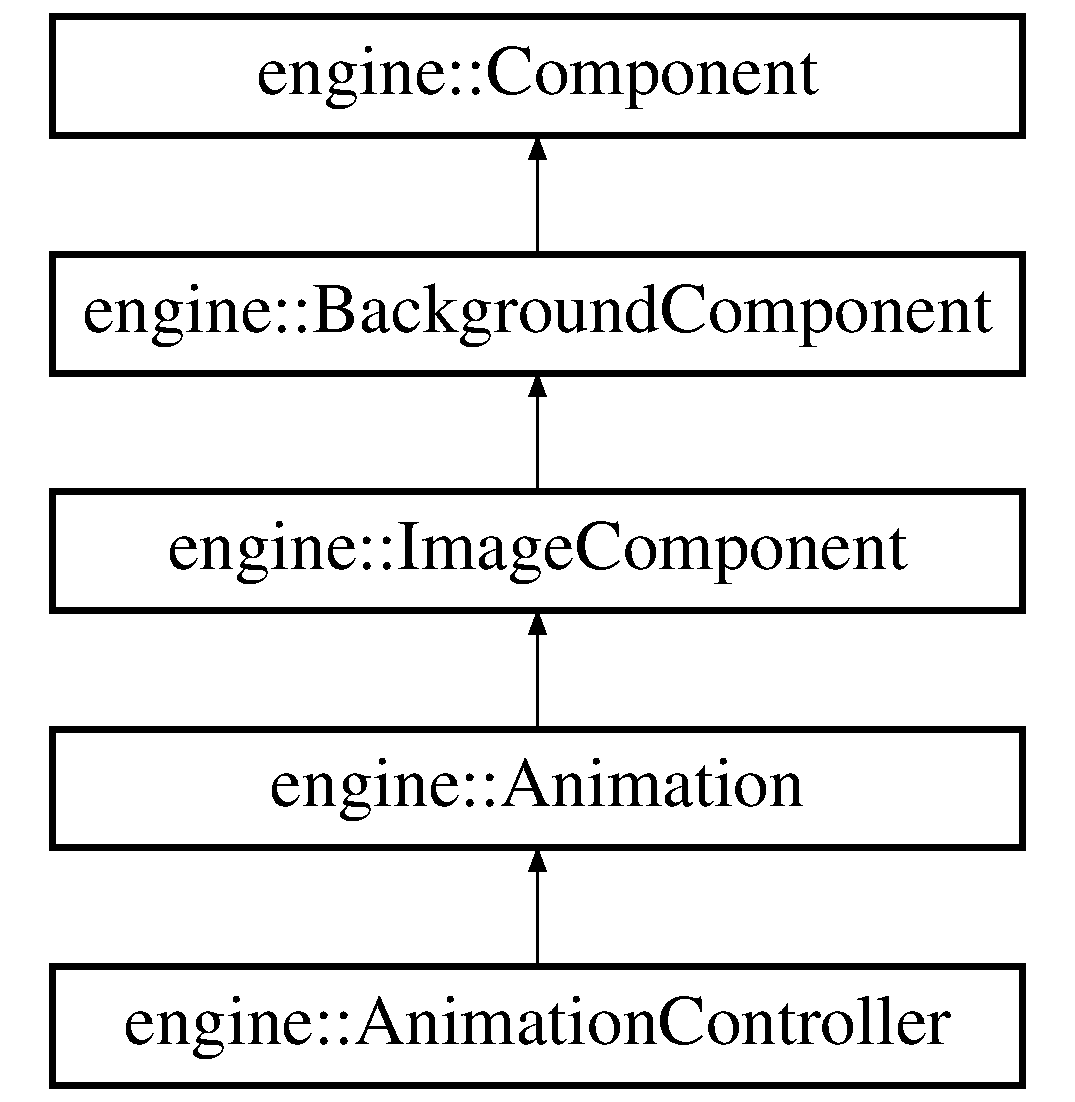
\includegraphics[height=5.000000cm]{classengine_1_1_image_component}
\end{center}
\end{figure}
\subsection*{Public Member Functions}
\begin{DoxyCompactItemize}
\item 
\hyperlink{classengine_1_1_image_component_a23b36883184415e68d4da77e06b10bf3}{Image\+Component} ()
\item 
virtual \hyperlink{classengine_1_1_image_component_a80d6f915909d151df0c785b803f1aafa}{$\sim$\+Image\+Component} ()
\item 
\hyperlink{classengine_1_1_image_component_ab6d7f27c64158fbea6ec71704abbf4ea}{Image\+Component} (\hyperlink{classengine_1_1_game_object}{Game\+Object} \&\hyperlink{classengine_1_1_component_ad4a4865ca4df98ebea34d04a4ec5ad07}{game\+Object}, std\+::string \hyperlink{classengine_1_1_background_component_aeffcb1aa8b67444e004413dee8c266b1}{image\+Path}, double \hyperlink{classengine_1_1_image_component_aa27852286227a84dc9c9f01c9fe2add8}{zoom\+Factor})
\item 
\hyperlink{classengine_1_1_image_component_acf18f670b8d344df162a50f76032ecfa}{Image\+Component} (\hyperlink{classengine_1_1_game_object}{Game\+Object} \&\hyperlink{classengine_1_1_component_ad4a4865ca4df98ebea34d04a4ec5ad07}{game\+Object}, std\+::string \hyperlink{classengine_1_1_background_component_aeffcb1aa8b67444e004413dee8c266b1}{image\+Path}, double \hyperlink{classengine_1_1_image_component_aa27852286227a84dc9c9f01c9fe2add8}{zoom\+Factor}, std\+::pair$<$ double, double $>$ position\+Relative\+To\+Object)
\item 
void \hyperlink{classengine_1_1_image_component_a4e5def28ca4647b29a4fe9bda78f9e57}{init} ()
\begin{DoxyCompactList}\small\item\em inherits function that initialize the game components \end{DoxyCompactList}\item 
void \hyperlink{classengine_1_1_image_component_a2be1a46da22f0f2280f7748c49fa6276}{draw} ()
\begin{DoxyCompactList}\small\item\em inherits function that draw game objects. \end{DoxyCompactList}\item 
void \hyperlink{classengine_1_1_image_component_ae821d9ce91c9cb6235b80d5ef248516b}{update\+Quad} ()
\item 
std\+::string \hyperlink{classengine_1_1_image_component_ac18bc924683d4d389b6706abd0afab20}{get\+Class\+Name} ()
\begin{DoxyCompactList}\small\item\em access the name of the class. \end{DoxyCompactList}\end{DoxyCompactItemize}
\subsection*{Protected Attributes}
\begin{DoxyCompactItemize}
\item 
std\+::pair$<$ double, double $>$ \hyperlink{classengine_1_1_image_component_aa89d785f15ac45a3b4343d08a2c5c146}{m\+Position\+Relative\+To\+Object} = std\+::make\+\_\+pair(0, 0)
\item 
double \hyperlink{classengine_1_1_image_component_aa27852286227a84dc9c9f01c9fe2add8}{zoom\+Factor}
\item 
S\+D\+L\+\_\+\+Rect \hyperlink{classengine_1_1_image_component_a563b4484c368c3206ce02a35b3cadd6b}{canvas\+Quad}
\end{DoxyCompactItemize}


\subsection{Detailed Description}


Definition at line 20 of file image\+\_\+component.\+hpp.



\subsection{Constructor \& Destructor Documentation}
\index{engine\+::\+Image\+Component@{engine\+::\+Image\+Component}!Image\+Component@{Image\+Component}}
\index{Image\+Component@{Image\+Component}!engine\+::\+Image\+Component@{engine\+::\+Image\+Component}}
\subsubsection[{\texorpdfstring{Image\+Component()}{ImageComponent()}}]{\setlength{\rightskip}{0pt plus 5cm}Image\+Component\+::\+Image\+Component (
\begin{DoxyParamCaption}
{}
\end{DoxyParamCaption}
)}\hypertarget{classengine_1_1_image_component_a23b36883184415e68d4da77e06b10bf3}{}\label{classengine_1_1_image_component_a23b36883184415e68d4da77e06b10bf3}


Definition at line 18 of file image\+\_\+component.\+cpp.

\index{engine\+::\+Image\+Component@{engine\+::\+Image\+Component}!````~Image\+Component@{$\sim$\+Image\+Component}}
\index{````~Image\+Component@{$\sim$\+Image\+Component}!engine\+::\+Image\+Component@{engine\+::\+Image\+Component}}
\subsubsection[{\texorpdfstring{$\sim$\+Image\+Component()}{~ImageComponent()}}]{\setlength{\rightskip}{0pt plus 5cm}Image\+Component\+::$\sim$\+Image\+Component (
\begin{DoxyParamCaption}
{}
\end{DoxyParamCaption}
)\hspace{0.3cm}{\ttfamily [virtual]}}\hypertarget{classengine_1_1_image_component_a80d6f915909d151df0c785b803f1aafa}{}\label{classengine_1_1_image_component_a80d6f915909d151df0c785b803f1aafa}


Definition at line 20 of file image\+\_\+component.\+cpp.

\index{engine\+::\+Image\+Component@{engine\+::\+Image\+Component}!Image\+Component@{Image\+Component}}
\index{Image\+Component@{Image\+Component}!engine\+::\+Image\+Component@{engine\+::\+Image\+Component}}
\subsubsection[{\texorpdfstring{Image\+Component(\+Game\+Object \&game\+Object, std\+::string image\+Path, double zoom\+Factor)}{ImageComponent(GameObject &gameObject, std::string imagePath, double zoomFactor)}}]{\setlength{\rightskip}{0pt plus 5cm}Image\+Component\+::\+Image\+Component (
\begin{DoxyParamCaption}
\item[{{\bf Game\+Object} \&}]{game\+Object, }
\item[{std\+::string}]{image\+Path, }
\item[{double}]{zoom\+Factor}
\end{DoxyParamCaption}
)}\hypertarget{classengine_1_1_image_component_ab6d7f27c64158fbea6ec71704abbf4ea}{}\label{classengine_1_1_image_component_ab6d7f27c64158fbea6ec71704abbf4ea}


Definition at line 22 of file image\+\_\+component.\+cpp.

\index{engine\+::\+Image\+Component@{engine\+::\+Image\+Component}!Image\+Component@{Image\+Component}}
\index{Image\+Component@{Image\+Component}!engine\+::\+Image\+Component@{engine\+::\+Image\+Component}}
\subsubsection[{\texorpdfstring{Image\+Component(\+Game\+Object \&game\+Object, std\+::string image\+Path, double zoom\+Factor, std\+::pair$<$ double, double $>$ position\+Relative\+To\+Object)}{ImageComponent(GameObject &gameObject, std::string imagePath, double zoomFactor, std::pair< double, double > positionRelativeToObject)}}]{\setlength{\rightskip}{0pt plus 5cm}Image\+Component\+::\+Image\+Component (
\begin{DoxyParamCaption}
\item[{{\bf Game\+Object} \&}]{game\+Object, }
\item[{std\+::string}]{image\+Path, }
\item[{double}]{zoom\+Factor, }
\item[{std\+::pair$<$ double, double $>$}]{position\+Relative\+To\+Object}
\end{DoxyParamCaption}
)}\hypertarget{classengine_1_1_image_component_acf18f670b8d344df162a50f76032ecfa}{}\label{classengine_1_1_image_component_acf18f670b8d344df162a50f76032ecfa}


Definition at line 28 of file image\+\_\+component.\+cpp.



\subsection{Member Function Documentation}
\index{engine\+::\+Image\+Component@{engine\+::\+Image\+Component}!draw@{draw}}
\index{draw@{draw}!engine\+::\+Image\+Component@{engine\+::\+Image\+Component}}
\subsubsection[{\texorpdfstring{draw()}{draw()}}]{\setlength{\rightskip}{0pt plus 5cm}void Image\+Component\+::draw (
\begin{DoxyParamCaption}
{}
\end{DoxyParamCaption}
)\hspace{0.3cm}{\ttfamily [virtual]}}\hypertarget{classengine_1_1_image_component_a2be1a46da22f0f2280f7748c49fa6276}{}\label{classengine_1_1_image_component_a2be1a46da22f0f2280f7748c49fa6276}


inherits function that draw game objects. 

draws all the enabled game objects.

\begin{DoxyReturn}{Returns}
\char`\"{}void\char`\"{}. 
\end{DoxyReturn}


Reimplemented from \hyperlink{classengine_1_1_background_component_a7b3c366c4b917888bde48917d83994be}{engine\+::\+Background\+Component}.



Definition at line 62 of file image\+\_\+component.\+cpp.

\index{engine\+::\+Image\+Component@{engine\+::\+Image\+Component}!get\+Class\+Name@{get\+Class\+Name}}
\index{get\+Class\+Name@{get\+Class\+Name}!engine\+::\+Image\+Component@{engine\+::\+Image\+Component}}
\subsubsection[{\texorpdfstring{get\+Class\+Name()}{getClassName()}}]{\setlength{\rightskip}{0pt plus 5cm}std\+::string engine\+::\+Image\+Component\+::get\+Class\+Name (
\begin{DoxyParamCaption}
{}
\end{DoxyParamCaption}
)\hspace{0.3cm}{\ttfamily [inline]}, {\ttfamily [virtual]}}\hypertarget{classengine_1_1_image_component_ac18bc924683d4d389b6706abd0afab20}{}\label{classengine_1_1_image_component_ac18bc924683d4d389b6706abd0afab20}


access the name of the class. 

Used to get the private attribute class\+Name.

\begin{DoxyReturn}{Returns}
string that contains the scene name. 
\end{DoxyReturn}


Reimplemented from \hyperlink{classengine_1_1_background_component_ad3283bbe6ab2d5c170ca67d2180c9fe2}{engine\+::\+Background\+Component}.



Definition at line 40 of file image\+\_\+component.\+hpp.

\index{engine\+::\+Image\+Component@{engine\+::\+Image\+Component}!init@{init}}
\index{init@{init}!engine\+::\+Image\+Component@{engine\+::\+Image\+Component}}
\subsubsection[{\texorpdfstring{init()}{init()}}]{\setlength{\rightskip}{0pt plus 5cm}void Image\+Component\+::init (
\begin{DoxyParamCaption}
{}
\end{DoxyParamCaption}
)\hspace{0.3cm}{\ttfamily [virtual]}}\hypertarget{classengine_1_1_image_component_a4e5def28ca4647b29a4fe9bda78f9e57}{}\label{classengine_1_1_image_component_a4e5def28ca4647b29a4fe9bda78f9e57}


inherits function that initialize the game components 

Set all game components to enable

\begin{DoxyReturn}{Returns}
\char`\"{}void\char`\"{}. 
\end{DoxyReturn}


Reimplemented from \hyperlink{classengine_1_1_background_component_a88a96b265f85934474d23d37cb2e6413}{engine\+::\+Background\+Component}.



Definition at line 38 of file image\+\_\+component.\+cpp.

\index{engine\+::\+Image\+Component@{engine\+::\+Image\+Component}!update\+Quad@{update\+Quad}}
\index{update\+Quad@{update\+Quad}!engine\+::\+Image\+Component@{engine\+::\+Image\+Component}}
\subsubsection[{\texorpdfstring{update\+Quad()}{updateQuad()}}]{\setlength{\rightskip}{0pt plus 5cm}void Image\+Component\+::update\+Quad (
\begin{DoxyParamCaption}
{}
\end{DoxyParamCaption}
)}\hypertarget{classengine_1_1_image_component_ae821d9ce91c9cb6235b80d5ef248516b}{}\label{classengine_1_1_image_component_ae821d9ce91c9cb6235b80d5ef248516b}


Definition at line 72 of file image\+\_\+component.\+cpp.



\subsection{Member Data Documentation}
\index{engine\+::\+Image\+Component@{engine\+::\+Image\+Component}!canvas\+Quad@{canvas\+Quad}}
\index{canvas\+Quad@{canvas\+Quad}!engine\+::\+Image\+Component@{engine\+::\+Image\+Component}}
\subsubsection[{\texorpdfstring{canvas\+Quad}{canvasQuad}}]{\setlength{\rightskip}{0pt plus 5cm}S\+D\+L\+\_\+\+Rect engine\+::\+Image\+Component\+::canvas\+Quad\hspace{0.3cm}{\ttfamily [protected]}}\hypertarget{classengine_1_1_image_component_a563b4484c368c3206ce02a35b3cadd6b}{}\label{classengine_1_1_image_component_a563b4484c368c3206ce02a35b3cadd6b}


Definition at line 24 of file image\+\_\+component.\+hpp.

\index{engine\+::\+Image\+Component@{engine\+::\+Image\+Component}!m\+Position\+Relative\+To\+Object@{m\+Position\+Relative\+To\+Object}}
\index{m\+Position\+Relative\+To\+Object@{m\+Position\+Relative\+To\+Object}!engine\+::\+Image\+Component@{engine\+::\+Image\+Component}}
\subsubsection[{\texorpdfstring{m\+Position\+Relative\+To\+Object}{mPositionRelativeToObject}}]{\setlength{\rightskip}{0pt plus 5cm}std\+::pair$<$double, double$>$ engine\+::\+Image\+Component\+::m\+Position\+Relative\+To\+Object = std\+::make\+\_\+pair(0, 0)\hspace{0.3cm}{\ttfamily [protected]}}\hypertarget{classengine_1_1_image_component_aa89d785f15ac45a3b4343d08a2c5c146}{}\label{classengine_1_1_image_component_aa89d785f15ac45a3b4343d08a2c5c146}


Definition at line 22 of file image\+\_\+component.\+hpp.

\index{engine\+::\+Image\+Component@{engine\+::\+Image\+Component}!zoom\+Factor@{zoom\+Factor}}
\index{zoom\+Factor@{zoom\+Factor}!engine\+::\+Image\+Component@{engine\+::\+Image\+Component}}
\subsubsection[{\texorpdfstring{zoom\+Factor}{zoomFactor}}]{\setlength{\rightskip}{0pt plus 5cm}double engine\+::\+Image\+Component\+::zoom\+Factor\hspace{0.3cm}{\ttfamily [protected]}}\hypertarget{classengine_1_1_image_component_aa27852286227a84dc9c9f01c9fe2add8}{}\label{classengine_1_1_image_component_aa27852286227a84dc9c9f01c9fe2add8}


Definition at line 23 of file image\+\_\+component.\+hpp.



The documentation for this class was generated from the following files\+:\begin{DoxyCompactItemize}
\item 
engine/include/\hyperlink{image__component_8hpp}{image\+\_\+component.\+hpp}\item 
engine/src/\hyperlink{image__component_8cpp}{image\+\_\+component.\+cpp}\end{DoxyCompactItemize}

\hypertarget{classengine_1_1_input_manager}{}\section{engine\+:\+:Input\+Manager Class Reference}
\label{classengine_1_1_input_manager}\index{engine\+::\+Input\+Manager@{engine\+::\+Input\+Manager}}


\hyperlink{classengine_1_1_input_manager}{Input\+Manager} class.  




{\ttfamily \#include $<$input\+\_\+manager.\+hpp$>$}

\subsection*{Public Member Functions}
\begin{DoxyCompactItemize}
\item 
\hyperlink{classengine_1_1_input_manager_a8be46886da639b26d67181c29dab6d6c}{Input\+Manager} ()
\begin{DoxyCompactList}\small\item\em Default constructor for the input manager. \end{DoxyCompactList}\item 
\hyperlink{classengine_1_1_input_manager_af518290877dd183606709d5852db5491}{$\sim$\+Input\+Manager} ()
\item 
void \hyperlink{classengine_1_1_input_manager_af7fdc23fa8b7bfa3651aa58f476b1a70}{update} (S\+D\+L\+\_\+\+Event \+\_\+event)
\begin{DoxyCompactList}\small\item\em update the sdl events. \end{DoxyCompactList}\item 
bool \hyperlink{classengine_1_1_input_manager_a3a25017b57aaa5ce61801158d852d1cb}{key\+Down} (\hyperlink{namespaceengine_ae215983ad6dd0b5102ec75314b5afe2d}{Button} button)
\begin{DoxyCompactList}\small\item\em test if button is pressed. \end{DoxyCompactList}\item 
bool \hyperlink{classengine_1_1_input_manager_ad82059c91ae6f43a6a5d5cd211b79c54}{key\+Down\+Once} (\hyperlink{namespaceengine_ae215983ad6dd0b5102ec75314b5afe2d}{Button} button)
\begin{DoxyCompactList}\small\item\em test if button is pressed once. \end{DoxyCompactList}\item 
bool \hyperlink{classengine_1_1_input_manager_a80d060705d719bd7f39329f7f34e32b8}{key\+State} (\hyperlink{namespaceengine_ae215983ad6dd0b5102ec75314b5afe2d}{Button} button)
\begin{DoxyCompactList}\small\item\em test the button state. \end{DoxyCompactList}\item 
void \hyperlink{classengine_1_1_input_manager_a233e9499354dc5c911a32a1f1d1f0ec0}{clear} ()
\begin{DoxyCompactList}\small\item\em clear. \end{DoxyCompactList}\end{DoxyCompactItemize}


\subsection{Detailed Description}
\hyperlink{classengine_1_1_input_manager}{Input\+Manager} class. 

This class is responsible for managing entries.

It works according to the command button that is selected. 

Definition at line 39 of file input\+\_\+manager.\+hpp.



\subsection{Constructor \& Destructor Documentation}
\index{engine\+::\+Input\+Manager@{engine\+::\+Input\+Manager}!Input\+Manager@{Input\+Manager}}
\index{Input\+Manager@{Input\+Manager}!engine\+::\+Input\+Manager@{engine\+::\+Input\+Manager}}
\subsubsection[{\texorpdfstring{Input\+Manager()}{InputManager()}}]{\setlength{\rightskip}{0pt plus 5cm}Input\+Manager\+::\+Input\+Manager (
\begin{DoxyParamCaption}
{}
\end{DoxyParamCaption}
)}\hypertarget{classengine_1_1_input_manager_a8be46886da639b26d67181c29dab6d6c}{}\label{classengine_1_1_input_manager_a8be46886da639b26d67181c29dab6d6c}


Default constructor for the input manager. 

\begin{DoxyReturn}{Returns}
\char`\"{}void\char`\"{}. 
\end{DoxyReturn}


Definition at line 19 of file input\+\_\+manager.\+cpp.

\index{engine\+::\+Input\+Manager@{engine\+::\+Input\+Manager}!````~Input\+Manager@{$\sim$\+Input\+Manager}}
\index{````~Input\+Manager@{$\sim$\+Input\+Manager}!engine\+::\+Input\+Manager@{engine\+::\+Input\+Manager}}
\subsubsection[{\texorpdfstring{$\sim$\+Input\+Manager()}{~InputManager()}}]{\setlength{\rightskip}{0pt plus 5cm}Input\+Manager\+::$\sim$\+Input\+Manager (
\begin{DoxyParamCaption}
{}
\end{DoxyParamCaption}
)}\hypertarget{classengine_1_1_input_manager_af518290877dd183606709d5852db5491}{}\label{classengine_1_1_input_manager_af518290877dd183606709d5852db5491}


Definition at line 20 of file input\+\_\+manager.\+cpp.



\subsection{Member Function Documentation}
\index{engine\+::\+Input\+Manager@{engine\+::\+Input\+Manager}!clear@{clear}}
\index{clear@{clear}!engine\+::\+Input\+Manager@{engine\+::\+Input\+Manager}}
\subsubsection[{\texorpdfstring{clear()}{clear()}}]{\setlength{\rightskip}{0pt plus 5cm}void Input\+Manager\+::clear (
\begin{DoxyParamCaption}
{}
\end{DoxyParamCaption}
)}\hypertarget{classengine_1_1_input_manager_a233e9499354dc5c911a32a1f1d1f0ec0}{}\label{classengine_1_1_input_manager_a233e9499354dc5c911a32a1f1d1f0ec0}


clear. 

Used to clear the events.

\begin{DoxyReturn}{Returns}
\char`\"{}void\char`\"{}. 
\end{DoxyReturn}


Definition at line 93 of file input\+\_\+manager.\+cpp.

\index{engine\+::\+Input\+Manager@{engine\+::\+Input\+Manager}!key\+Down@{key\+Down}}
\index{key\+Down@{key\+Down}!engine\+::\+Input\+Manager@{engine\+::\+Input\+Manager}}
\subsubsection[{\texorpdfstring{key\+Down(\+Button button)}{keyDown(Button button)}}]{\setlength{\rightskip}{0pt plus 5cm}bool Input\+Manager\+::key\+Down (
\begin{DoxyParamCaption}
\item[{{\bf Button}}]{button}
\end{DoxyParamCaption}
)}\hypertarget{classengine_1_1_input_manager_a3a25017b57aaa5ce61801158d852d1cb}{}\label{classengine_1_1_input_manager_a3a25017b57aaa5ce61801158d852d1cb}


test if button is pressed. 

Used to set the test of key down.


\begin{DoxyParams}{Parameters}
{\em Button} & that represent user input.\\
\hline
\end{DoxyParams}
\begin{DoxyReturn}{Returns}
a bool that indicates the add scene success. 
\end{DoxyReturn}


Definition at line 31 of file input\+\_\+manager.\+cpp.

\index{engine\+::\+Input\+Manager@{engine\+::\+Input\+Manager}!key\+Down\+Once@{key\+Down\+Once}}
\index{key\+Down\+Once@{key\+Down\+Once}!engine\+::\+Input\+Manager@{engine\+::\+Input\+Manager}}
\subsubsection[{\texorpdfstring{key\+Down\+Once(\+Button button)}{keyDownOnce(Button button)}}]{\setlength{\rightskip}{0pt plus 5cm}bool Input\+Manager\+::key\+Down\+Once (
\begin{DoxyParamCaption}
\item[{{\bf Button}}]{button}
\end{DoxyParamCaption}
)}\hypertarget{classengine_1_1_input_manager_ad82059c91ae6f43a6a5d5cd211b79c54}{}\label{classengine_1_1_input_manager_ad82059c91ae6f43a6a5d5cd211b79c54}


test if button is pressed once. 

Used to set the test of key down only once.


\begin{DoxyParams}{Parameters}
{\em Button} & that represent user input.\\
\hline
\end{DoxyParams}
\begin{DoxyReturn}{Returns}
a bool that indicates the add scene success. 
\end{DoxyReturn}


Definition at line 61 of file input\+\_\+manager.\+cpp.

\index{engine\+::\+Input\+Manager@{engine\+::\+Input\+Manager}!key\+State@{key\+State}}
\index{key\+State@{key\+State}!engine\+::\+Input\+Manager@{engine\+::\+Input\+Manager}}
\subsubsection[{\texorpdfstring{key\+State(\+Button button)}{keyState(Button button)}}]{\setlength{\rightskip}{0pt plus 5cm}bool Input\+Manager\+::key\+State (
\begin{DoxyParamCaption}
\item[{{\bf Button}}]{button}
\end{DoxyParamCaption}
)}\hypertarget{classengine_1_1_input_manager_a80d060705d719bd7f39329f7f34e32b8}{}\label{classengine_1_1_input_manager_a80d060705d719bd7f39329f7f34e32b8}


test the button state. 

Used to set the test of key state.


\begin{DoxyParams}{Parameters}
{\em Button} & that represent user input.\\
\hline
\end{DoxyParams}
\begin{DoxyReturn}{Returns}
a bool that indicates the add scene success. 
\end{DoxyReturn}


Definition at line 80 of file input\+\_\+manager.\+cpp.

\index{engine\+::\+Input\+Manager@{engine\+::\+Input\+Manager}!update@{update}}
\index{update@{update}!engine\+::\+Input\+Manager@{engine\+::\+Input\+Manager}}
\subsubsection[{\texorpdfstring{update(\+S\+D\+L\+\_\+\+Event \+\_\+event)}{update(SDL_Event _event)}}]{\setlength{\rightskip}{0pt plus 5cm}void Input\+Manager\+::update (
\begin{DoxyParamCaption}
\item[{S\+D\+L\+\_\+\+Event}]{\+\_\+event}
\end{DoxyParamCaption}
)}\hypertarget{classengine_1_1_input_manager_af7fdc23fa8b7bfa3651aa58f476b1a70}{}\label{classengine_1_1_input_manager_af7fdc23fa8b7bfa3651aa58f476b1a70}


update the sdl events. 

Used to get the keyboard state.


\begin{DoxyParams}{Parameters}
{\em \+\_\+event.} & \\
\hline
\end{DoxyParams}
\begin{DoxyReturn}{Returns}
\char`\"{}void\char`\"{}. 
\end{DoxyReturn}


Definition at line 106 of file input\+\_\+manager.\+cpp.



The documentation for this class was generated from the following files\+:\begin{DoxyCompactItemize}
\item 
engine/include/\hyperlink{input__manager_8hpp}{input\+\_\+manager.\+hpp}\item 
engine/src/\hyperlink{input__manager_8cpp}{input\+\_\+manager.\+cpp}\end{DoxyCompactItemize}

\hypertarget{class_azo_1_1_invisible_block}{}\section{Azo\+:\+:Invisible\+Block Class Reference}
\label{class_azo_1_1_invisible_block}\index{Azo\+::\+Invisible\+Block@{Azo\+::\+Invisible\+Block}}


A collision class with invisible blocks.  




{\ttfamily \#include $<$invisible\+\_\+block.\+hpp$>$}

Inheritance diagram for Azo\+:\+:Invisible\+Block\+:\begin{figure}[H]
\begin{center}
\leavevmode
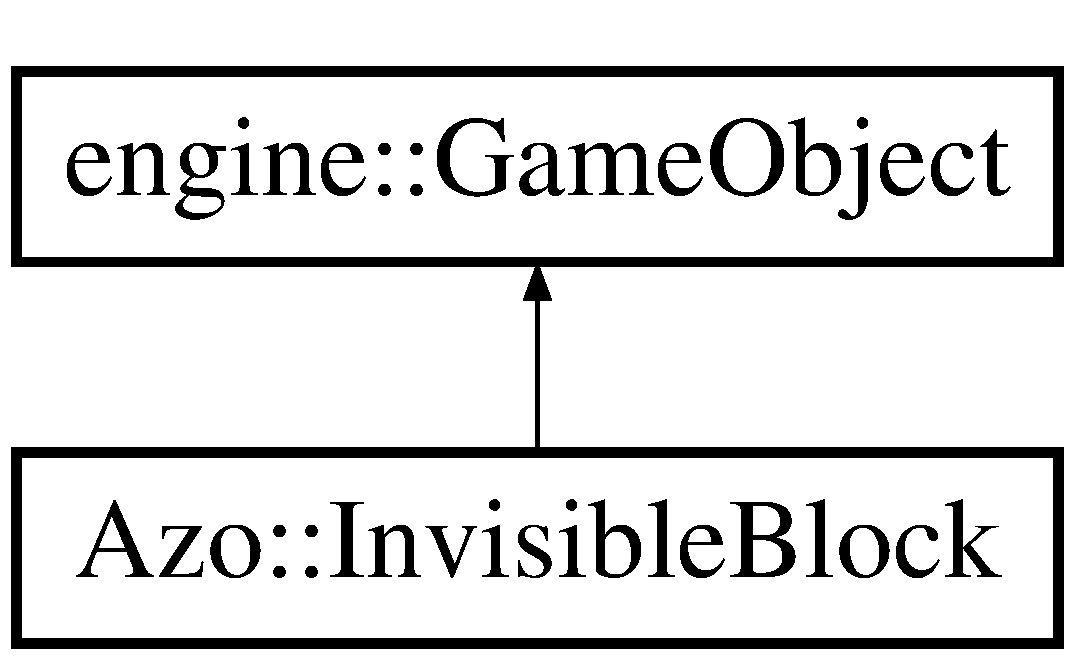
\includegraphics[height=2.000000cm]{class_azo_1_1_invisible_block}
\end{center}
\end{figure}
\subsection*{Public Member Functions}
\begin{DoxyCompactItemize}
\item 
\hyperlink{class_azo_1_1_invisible_block_a75b3abaaaa5dd90bf39a83b1605dd9ad}{Invisible\+Block} ()
\item 
virtual \hyperlink{class_azo_1_1_invisible_block_a08325dc2f5ef563800beaa2a6bc73667}{$\sim$\+Invisible\+Block} ()
\item 
\hyperlink{class_azo_1_1_invisible_block_ab47f9aabb5bd98f2159b188ab4d29ede}{Invisible\+Block} (std\+::string name, std\+::pair$<$ double, double $>$ position\+Relative\+To\+Parent, std\+::pair$<$ double, double $>$ size)
\begin{DoxyCompactList}\small\item\em Constructor for \hyperlink{class_azo_1_1_invisible_block}{Invisible\+Block} class. \end{DoxyCompactList}\item 
void \hyperlink{class_azo_1_1_invisible_block_adeb8f56bc48b28236165da3ef05af0b1}{shutdown} ()
\begin{DoxyCompactList}\small\item\em Destructor class for \hyperlink{class_azo_1_1_invisible_block}{Invisible\+Block}. \end{DoxyCompactList}\item 
std\+::string \hyperlink{class_azo_1_1_invisible_block_a627cab09cdae548b6d58ceb150561a45}{get\+Class\+Name} ()
\begin{DoxyCompactList}\small\item\em Method for class name. \end{DoxyCompactList}\end{DoxyCompactItemize}
\subsection*{Public Attributes}
\begin{DoxyCompactItemize}
\item 
std\+::pair$<$ double, double $>$ \hyperlink{class_azo_1_1_invisible_block_aa761a24addda645a72ecc5b8db29095d}{m\+Position\+Relative\+To\+Parent}
\end{DoxyCompactItemize}
\subsection*{Additional Inherited Members}


\subsection{Detailed Description}
A collision class with invisible blocks. 

A class for collision calculation using invisible blocks as parameters. 

Definition at line 21 of file invisible\+\_\+block.\+hpp.



\subsection{Constructor \& Destructor Documentation}
\index{Azo\+::\+Invisible\+Block@{Azo\+::\+Invisible\+Block}!Invisible\+Block@{Invisible\+Block}}
\index{Invisible\+Block@{Invisible\+Block}!Azo\+::\+Invisible\+Block@{Azo\+::\+Invisible\+Block}}
\subsubsection[{\texorpdfstring{Invisible\+Block()}{InvisibleBlock()}}]{\setlength{\rightskip}{0pt plus 5cm}Azo\+::\+Invisible\+Block\+::\+Invisible\+Block (
\begin{DoxyParamCaption}
{}
\end{DoxyParamCaption}
)}\hypertarget{class_azo_1_1_invisible_block_a75b3abaaaa5dd90bf39a83b1605dd9ad}{}\label{class_azo_1_1_invisible_block_a75b3abaaaa5dd90bf39a83b1605dd9ad}
\index{Azo\+::\+Invisible\+Block@{Azo\+::\+Invisible\+Block}!````~Invisible\+Block@{$\sim$\+Invisible\+Block}}
\index{````~Invisible\+Block@{$\sim$\+Invisible\+Block}!Azo\+::\+Invisible\+Block@{Azo\+::\+Invisible\+Block}}
\subsubsection[{\texorpdfstring{$\sim$\+Invisible\+Block()}{~InvisibleBlock()}}]{\setlength{\rightskip}{0pt plus 5cm}Invisible\+Block\+::$\sim$\+Invisible\+Block (
\begin{DoxyParamCaption}
{}
\end{DoxyParamCaption}
)\hspace{0.3cm}{\ttfamily [virtual]}}\hypertarget{class_azo_1_1_invisible_block_a08325dc2f5ef563800beaa2a6bc73667}{}\label{class_azo_1_1_invisible_block_a08325dc2f5ef563800beaa2a6bc73667}


Definition at line 14 of file invisible\+\_\+block.\+cpp.

\index{Azo\+::\+Invisible\+Block@{Azo\+::\+Invisible\+Block}!Invisible\+Block@{Invisible\+Block}}
\index{Invisible\+Block@{Invisible\+Block}!Azo\+::\+Invisible\+Block@{Azo\+::\+Invisible\+Block}}
\subsubsection[{\texorpdfstring{Invisible\+Block(std\+::string name, std\+::pair$<$ double, double $>$ position\+Relative\+To\+Parent, std\+::pair$<$ double, double $>$ size)}{InvisibleBlock(std::string name, std::pair< double, double > positionRelativeToParent, std::pair< double, double > size)}}]{\setlength{\rightskip}{0pt plus 5cm}Invisible\+Block\+::\+Invisible\+Block (
\begin{DoxyParamCaption}
\item[{std\+::string}]{name, }
\item[{std\+::pair$<$ double, double $>$}]{position\+Relative\+To\+Parent, }
\item[{std\+::pair$<$ double, double $>$}]{size}
\end{DoxyParamCaption}
)}\hypertarget{class_azo_1_1_invisible_block_ab47f9aabb5bd98f2159b188ab4d29ede}{}\label{class_azo_1_1_invisible_block_ab47f9aabb5bd98f2159b188ab4d29ede}


Constructor for \hyperlink{class_azo_1_1_invisible_block}{Invisible\+Block} class. 

Used for initializing class variables. 
\begin{DoxyParams}{Parameters}
{\em name} & \hyperlink{class_azo_1_1_invisible_block}{Invisible\+Block} name. \\
\hline
{\em position\+Relative\+To\+Parent} & Pair of doubles relative to position(range $>$ 0). \\
\hline
{\em size} & Pair of doubles relative to size(range $>$ 0). \\
\hline
\end{DoxyParams}


Definition at line 24 of file invisible\+\_\+block.\+cpp.



\subsection{Member Function Documentation}
\index{Azo\+::\+Invisible\+Block@{Azo\+::\+Invisible\+Block}!get\+Class\+Name@{get\+Class\+Name}}
\index{get\+Class\+Name@{get\+Class\+Name}!Azo\+::\+Invisible\+Block@{Azo\+::\+Invisible\+Block}}
\subsubsection[{\texorpdfstring{get\+Class\+Name()}{getClassName()}}]{\setlength{\rightskip}{0pt plus 5cm}std\+::string Azo\+::\+Invisible\+Block\+::get\+Class\+Name (
\begin{DoxyParamCaption}
{}
\end{DoxyParamCaption}
)\hspace{0.3cm}{\ttfamily [inline]}, {\ttfamily [virtual]}}\hypertarget{class_azo_1_1_invisible_block_a627cab09cdae548b6d58ceb150561a45}{}\label{class_azo_1_1_invisible_block_a627cab09cdae548b6d58ceb150561a45}


Method for class name. 

Inline method for returning the class\textquotesingle{} name. 

Reimplemented from \hyperlink{classengine_1_1_game_object_ac836deb7933c725ac09b67386ad10239}{engine\+::\+Game\+Object}.



Definition at line 38 of file invisible\+\_\+block.\+hpp.

\index{Azo\+::\+Invisible\+Block@{Azo\+::\+Invisible\+Block}!shutdown@{shutdown}}
\index{shutdown@{shutdown}!Azo\+::\+Invisible\+Block@{Azo\+::\+Invisible\+Block}}
\subsubsection[{\texorpdfstring{shutdown()}{shutdown()}}]{\setlength{\rightskip}{0pt plus 5cm}void Invisible\+Block\+::shutdown (
\begin{DoxyParamCaption}
{}
\end{DoxyParamCaption}
)\hspace{0.3cm}{\ttfamily [virtual]}}\hypertarget{class_azo_1_1_invisible_block_adeb8f56bc48b28236165da3ef05af0b1}{}\label{class_azo_1_1_invisible_block_adeb8f56bc48b28236165da3ef05af0b1}


Destructor class for \hyperlink{class_azo_1_1_invisible_block}{Invisible\+Block}. 

Used for shutting down Image\+Component so as to free memory when closing the game. 

Reimplemented from \hyperlink{classengine_1_1_game_object_a08d7a48b6eb90f55c8b670b6f98ab393}{engine\+::\+Game\+Object}.



Definition at line 51 of file invisible\+\_\+block.\+cpp.



\subsection{Member Data Documentation}
\index{Azo\+::\+Invisible\+Block@{Azo\+::\+Invisible\+Block}!m\+Position\+Relative\+To\+Parent@{m\+Position\+Relative\+To\+Parent}}
\index{m\+Position\+Relative\+To\+Parent@{m\+Position\+Relative\+To\+Parent}!Azo\+::\+Invisible\+Block@{Azo\+::\+Invisible\+Block}}
\subsubsection[{\texorpdfstring{m\+Position\+Relative\+To\+Parent}{mPositionRelativeToParent}}]{\setlength{\rightskip}{0pt plus 5cm}std\+::pair$<$double, double$>$ Azo\+::\+Invisible\+Block\+::m\+Position\+Relative\+To\+Parent}\hypertarget{class_azo_1_1_invisible_block_aa761a24addda645a72ecc5b8db29095d}{}\label{class_azo_1_1_invisible_block_aa761a24addda645a72ecc5b8db29095d}


Definition at line 26 of file invisible\+\_\+block.\+hpp.



The documentation for this class was generated from the following files\+:\begin{DoxyCompactItemize}
\item 
include/\hyperlink{invisible__block_8hpp}{invisible\+\_\+block.\+hpp}\item 
src/\hyperlink{invisible__block_8cpp}{invisible\+\_\+block.\+cpp}\end{DoxyCompactItemize}

\hypertarget{class_azo_1_1_level_one}{}\section{Azo\+:\+:Level\+One Class Reference}
\label{class_azo_1_1_level_one}\index{Azo\+::\+Level\+One@{Azo\+::\+Level\+One}}


\hyperlink{class_azo_1_1_level_one}{Level\+One} class This class is used to manage creation and behavior of game objects, menus and parents.  




{\ttfamily \#include $<$level\+\_\+one.\+hpp$>$}

Inheritance diagram for Azo\+:\+:Level\+One\+:\begin{figure}[H]
\begin{center}
\leavevmode
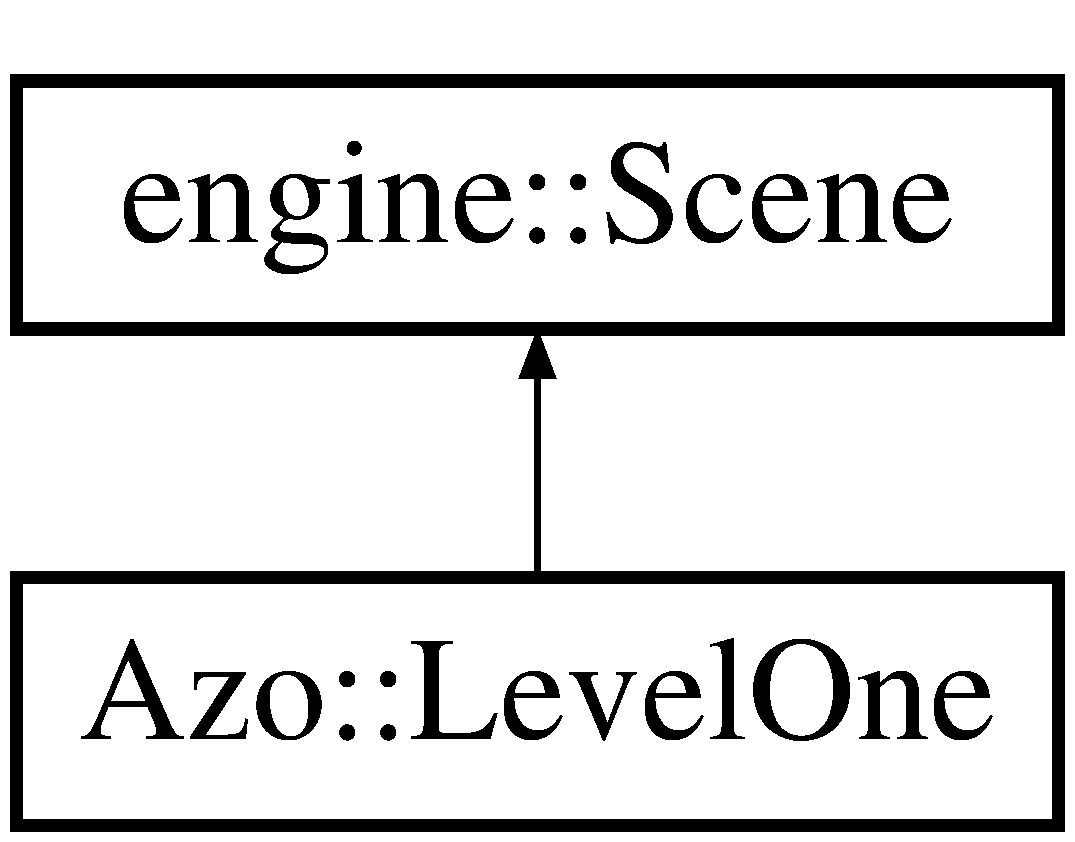
\includegraphics[height=2.000000cm]{class_azo_1_1_level_one}
\end{center}
\end{figure}
\subsection*{Public Member Functions}
\begin{DoxyCompactItemize}
\item 
\hyperlink{class_azo_1_1_level_one_a3fe4df62466654e6e7617377c8bd67a7}{Level\+One} ()
\item 
\hyperlink{class_azo_1_1_level_one_a7162ded32f3cc966d0e3304666beb878}{Level\+One} (std\+::string name)
\item 
void \hyperlink{class_azo_1_1_level_one_ac388145a996f6663e2ae757f026f07f1}{restart} ()
\end{DoxyCompactItemize}
\subsection*{Additional Inherited Members}


\subsection{Detailed Description}
\hyperlink{class_azo_1_1_level_one}{Level\+One} class This class is used to manage creation and behavior of game objects, menus and parents. 

Definition at line 28 of file level\+\_\+one.\+hpp.



\subsection{Constructor \& Destructor Documentation}
\index{Azo\+::\+Level\+One@{Azo\+::\+Level\+One}!Level\+One@{Level\+One}}
\index{Level\+One@{Level\+One}!Azo\+::\+Level\+One@{Azo\+::\+Level\+One}}
\subsubsection[{\texorpdfstring{Level\+One()}{LevelOne()}}]{\setlength{\rightskip}{0pt plus 5cm}Level\+One\+::\+Level\+One (
\begin{DoxyParamCaption}
{}
\end{DoxyParamCaption}
)}\hypertarget{class_azo_1_1_level_one_a3fe4df62466654e6e7617377c8bd67a7}{}\label{class_azo_1_1_level_one_a3fe4df62466654e6e7617377c8bd67a7}


Definition at line 16 of file level\+\_\+one.\+cpp.

\index{Azo\+::\+Level\+One@{Azo\+::\+Level\+One}!Level\+One@{Level\+One}}
\index{Level\+One@{Level\+One}!Azo\+::\+Level\+One@{Azo\+::\+Level\+One}}
\subsubsection[{\texorpdfstring{Level\+One(std\+::string name)}{LevelOne(std::string name)}}]{\setlength{\rightskip}{0pt plus 5cm}Level\+One\+::\+Level\+One (
\begin{DoxyParamCaption}
\item[{std\+::string}]{name}
\end{DoxyParamCaption}
)}\hypertarget{class_azo_1_1_level_one_a7162ded32f3cc966d0e3304666beb878}{}\label{class_azo_1_1_level_one_a7162ded32f3cc966d0e3304666beb878}


Definition at line 19 of file level\+\_\+one.\+cpp.



\subsection{Member Function Documentation}
\index{Azo\+::\+Level\+One@{Azo\+::\+Level\+One}!restart@{restart}}
\index{restart@{restart}!Azo\+::\+Level\+One@{Azo\+::\+Level\+One}}
\subsubsection[{\texorpdfstring{restart()}{restart()}}]{\setlength{\rightskip}{0pt plus 5cm}void Level\+One\+::restart (
\begin{DoxyParamCaption}
{}
\end{DoxyParamCaption}
)\hspace{0.3cm}{\ttfamily [virtual]}}\hypertarget{class_azo_1_1_level_one_ac388145a996f6663e2ae757f026f07f1}{}\label{class_azo_1_1_level_one_ac388145a996f6663e2ae757f026f07f1}


Reimplemented from \hyperlink{classengine_1_1_scene_a279192188f7c239355209afd3e7c16ac}{engine\+::\+Scene}.



Definition at line 25 of file level\+\_\+one.\+cpp.



The documentation for this class was generated from the following files\+:\begin{DoxyCompactItemize}
\item 
include/\hyperlink{level__one_8hpp}{level\+\_\+one.\+hpp}\item 
src/\hyperlink{level__one_8cpp}{level\+\_\+one.\+cpp}\end{DoxyCompactItemize}

\hypertarget{class_azo_1_1_level_one_code}{}\section{Azo\+:\+:Level\+One\+Code Class Reference}
\label{class_azo_1_1_level_one_code}\index{Azo\+::\+Level\+One\+Code@{Azo\+::\+Level\+One\+Code}}


\hyperlink{class_azo_1_1_level_one_code}{Level\+One\+Code} class This class is used to manage creation and behavior of the engine at the first level of the game.  




{\ttfamily \#include $<$level\+\_\+one\+\_\+code.\+hpp$>$}

Inheritance diagram for Azo\+:\+:Level\+One\+Code\+:\begin{figure}[H]
\begin{center}
\leavevmode
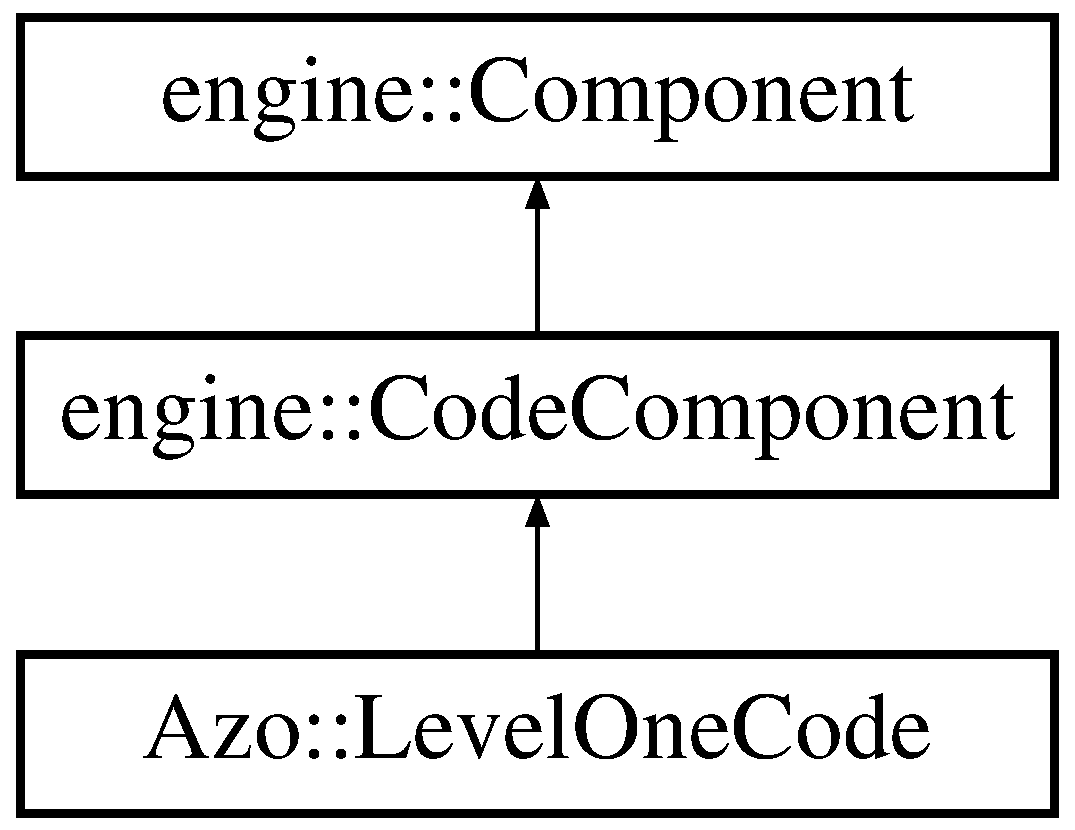
\includegraphics[height=3.000000cm]{class_azo_1_1_level_one_code}
\end{center}
\end{figure}
\subsection*{Public Member Functions}
\begin{DoxyCompactItemize}
\item 
\hyperlink{class_azo_1_1_level_one_code_aa35d7bc4e322a0db629dcdbdd60c07ca}{Level\+One\+Code} (\hyperlink{classengine_1_1_game_object}{engine\+::\+Game\+Object} \&\hyperlink{classengine_1_1_component_ad4a4865ca4df98ebea34d04a4ec5ad07}{game\+Object})
\item 
void \hyperlink{class_azo_1_1_level_one_code_af66d92f836d8a6c0f72d718d05db63a5}{shutdown} ()
\begin{DoxyCompactList}\small\item\em inherits function that disable the game code components. \end{DoxyCompactList}\end{DoxyCompactItemize}
\subsection*{Additional Inherited Members}


\subsection{Detailed Description}
\hyperlink{class_azo_1_1_level_one_code}{Level\+One\+Code} class This class is used to manage creation and behavior of the engine at the first level of the game. 

Definition at line 26 of file level\+\_\+one\+\_\+code.\+hpp.



\subsection{Constructor \& Destructor Documentation}
\index{Azo\+::\+Level\+One\+Code@{Azo\+::\+Level\+One\+Code}!Level\+One\+Code@{Level\+One\+Code}}
\index{Level\+One\+Code@{Level\+One\+Code}!Azo\+::\+Level\+One\+Code@{Azo\+::\+Level\+One\+Code}}
\subsubsection[{\texorpdfstring{Level\+One\+Code(engine\+::\+Game\+Object \&game\+Object)}{LevelOneCode(engine::GameObject &gameObject)}}]{\setlength{\rightskip}{0pt plus 5cm}Level\+One\+Code\+::\+Level\+One\+Code (
\begin{DoxyParamCaption}
\item[{{\bf engine\+::\+Game\+Object} \&}]{game\+Object}
\end{DoxyParamCaption}
)}\hypertarget{class_azo_1_1_level_one_code_aa35d7bc4e322a0db629dcdbdd60c07ca}{}\label{class_azo_1_1_level_one_code_aa35d7bc4e322a0db629dcdbdd60c07ca}


Definition at line 16 of file level\+\_\+one\+\_\+code.\+cpp.



\subsection{Member Function Documentation}
\index{Azo\+::\+Level\+One\+Code@{Azo\+::\+Level\+One\+Code}!shutdown@{shutdown}}
\index{shutdown@{shutdown}!Azo\+::\+Level\+One\+Code@{Azo\+::\+Level\+One\+Code}}
\subsubsection[{\texorpdfstring{shutdown()}{shutdown()}}]{\setlength{\rightskip}{0pt plus 5cm}void Level\+One\+Code\+::shutdown (
\begin{DoxyParamCaption}
{}
\end{DoxyParamCaption}
)\hspace{0.3cm}{\ttfamily [virtual]}}\hypertarget{class_azo_1_1_level_one_code_af66d92f836d8a6c0f72d718d05db63a5}{}\label{class_azo_1_1_level_one_code_af66d92f836d8a6c0f72d718d05db63a5}


inherits function that disable the game code components. 

free the code component pointer.

\begin{DoxyReturn}{Returns}
\char`\"{}void\char`\"{}. 
\end{DoxyReturn}


Reimplemented from \hyperlink{classengine_1_1_code_component_af76ba17f9f87216418081d1e2c7c3a22}{engine\+::\+Code\+Component}.



Definition at line 22 of file level\+\_\+one\+\_\+code.\+cpp.



The documentation for this class was generated from the following files\+:\begin{DoxyCompactItemize}
\item 
include/\hyperlink{level__one__code_8hpp}{level\+\_\+one\+\_\+code.\+hpp}\item 
src/\hyperlink{level__one__code_8cpp}{level\+\_\+one\+\_\+code.\+cpp}\end{DoxyCompactItemize}

\hypertarget{class_azo_1_1_machine_part_code}{}\section{Azo\+:\+:Machine\+Part\+Code Class Reference}
\label{class_azo_1_1_machine_part_code}\index{Azo\+::\+Machine\+Part\+Code@{Azo\+::\+Machine\+Part\+Code}}


A Hitbox class. \hyperlink{class_azo_1_1_machine_part_code}{Machine\+Part\+Code} class.  




{\ttfamily \#include $<$machine\+\_\+part\+\_\+code.\+hpp$>$}

Inheritance diagram for Azo\+:\+:Machine\+Part\+Code\+:\begin{figure}[H]
\begin{center}
\leavevmode
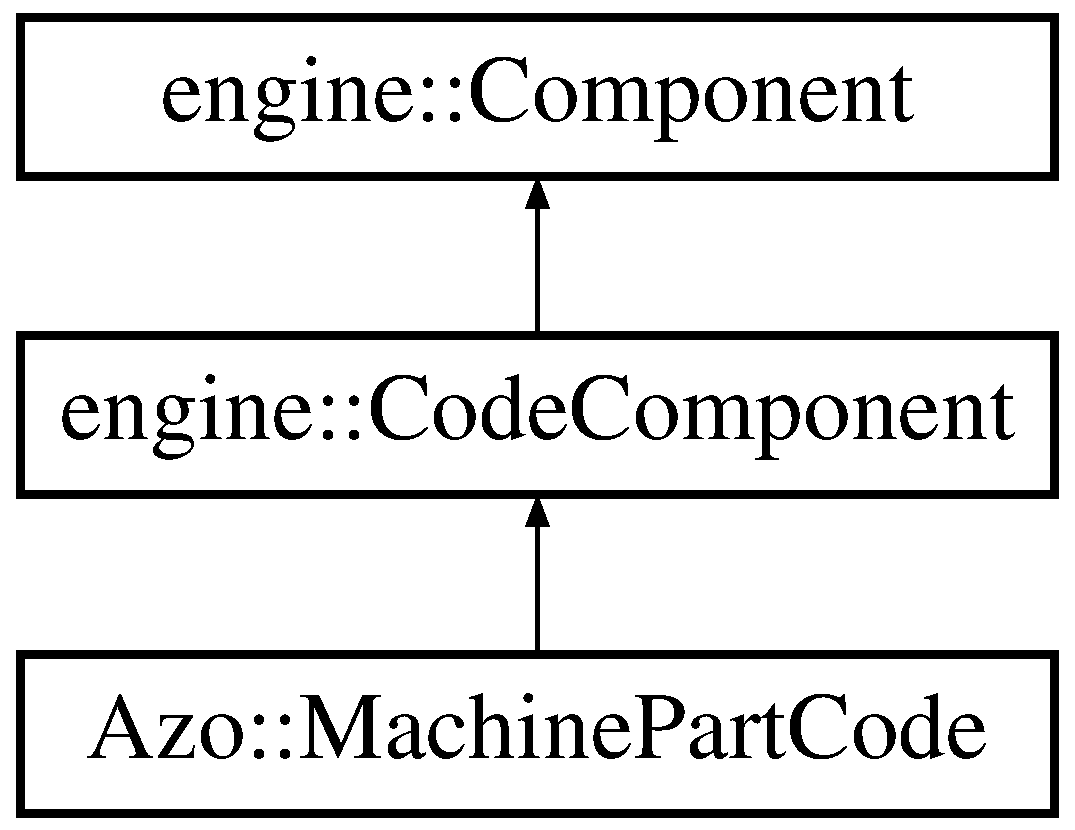
\includegraphics[height=3.000000cm]{class_azo_1_1_machine_part_code}
\end{center}
\end{figure}
\subsection*{Public Member Functions}
\begin{DoxyCompactItemize}
\item 
\hyperlink{class_azo_1_1_machine_part_code_a4ce37129563be975a557942ab8c897f0}{Machine\+Part\+Code} (\hyperlink{class_azo_1_1_obstacle}{Obstacle} $\ast$machine\+Part)
\begin{DoxyCompactList}\small\item\em function responsible for creating parts that will be collected by the player \end{DoxyCompactList}\item 
virtual \hyperlink{class_azo_1_1_machine_part_code_a3769b1d5af7d63b989369aef122760b5}{$\sim$\+Machine\+Part\+Code} ()
\item 
void \hyperlink{class_azo_1_1_machine_part_code_aea9e8e5ccc20e0ac975277104b29d0bf}{shutdown} ()
\begin{DoxyCompactList}\small\item\em function responsible for disabling game audio \end{DoxyCompactList}\end{DoxyCompactItemize}
\subsection*{Additional Inherited Members}


\subsection{Detailed Description}
A Hitbox class. \hyperlink{class_azo_1_1_machine_part_code}{Machine\+Part\+Code} class. 

A more elaborate class description. Class responsible for the creation of the parts by which the player must collect to get to victory. 

Definition at line 27 of file machine\+\_\+part\+\_\+code.\+hpp.



\subsection{Constructor \& Destructor Documentation}
\index{Azo\+::\+Machine\+Part\+Code@{Azo\+::\+Machine\+Part\+Code}!Machine\+Part\+Code@{Machine\+Part\+Code}}
\index{Machine\+Part\+Code@{Machine\+Part\+Code}!Azo\+::\+Machine\+Part\+Code@{Azo\+::\+Machine\+Part\+Code}}
\subsubsection[{\texorpdfstring{Machine\+Part\+Code(\+Obstacle $\ast$machine\+Part)}{MachinePartCode(Obstacle *machinePart)}}]{\setlength{\rightskip}{0pt plus 5cm}Machine\+Part\+Code\+::\+Machine\+Part\+Code (
\begin{DoxyParamCaption}
\item[{{\bf Obstacle} $\ast$}]{machine\+Part}
\end{DoxyParamCaption}
)}\hypertarget{class_azo_1_1_machine_part_code_a4ce37129563be975a557942ab8c897f0}{}\label{class_azo_1_1_machine_part_code_a4ce37129563be975a557942ab8c897f0}


function responsible for creating parts that will be collected by the player 

Why\+: So that they can be collected throughout the game by the player


\begin{DoxyParams}{Parameters}
{\em \hyperlink{class_azo_1_1_obstacle}{Obstacle}} & that has the parts that need to be collected \\
\hline
\end{DoxyParams}


Definition at line 23 of file machine\+\_\+part\+\_\+code.\+cpp.

\index{Azo\+::\+Machine\+Part\+Code@{Azo\+::\+Machine\+Part\+Code}!````~Machine\+Part\+Code@{$\sim$\+Machine\+Part\+Code}}
\index{````~Machine\+Part\+Code@{$\sim$\+Machine\+Part\+Code}!Azo\+::\+Machine\+Part\+Code@{Azo\+::\+Machine\+Part\+Code}}
\subsubsection[{\texorpdfstring{$\sim$\+Machine\+Part\+Code()}{~MachinePartCode()}}]{\setlength{\rightskip}{0pt plus 5cm}Machine\+Part\+Code\+::$\sim$\+Machine\+Part\+Code (
\begin{DoxyParamCaption}
{}
\end{DoxyParamCaption}
)\hspace{0.3cm}{\ttfamily [virtual]}}\hypertarget{class_azo_1_1_machine_part_code_a3769b1d5af7d63b989369aef122760b5}{}\label{class_azo_1_1_machine_part_code_a3769b1d5af7d63b989369aef122760b5}


Definition at line 28 of file machine\+\_\+part\+\_\+code.\+cpp.



\subsection{Member Function Documentation}
\index{Azo\+::\+Machine\+Part\+Code@{Azo\+::\+Machine\+Part\+Code}!shutdown@{shutdown}}
\index{shutdown@{shutdown}!Azo\+::\+Machine\+Part\+Code@{Azo\+::\+Machine\+Part\+Code}}
\subsubsection[{\texorpdfstring{shutdown()}{shutdown()}}]{\setlength{\rightskip}{0pt plus 5cm}void Machine\+Part\+Code\+::shutdown (
\begin{DoxyParamCaption}
{}
\end{DoxyParamCaption}
)\hspace{0.3cm}{\ttfamily [virtual]}}\hypertarget{class_azo_1_1_machine_part_code_aea9e8e5ccc20e0ac975277104b29d0bf}{}\label{class_azo_1_1_machine_part_code_aea9e8e5ccc20e0ac975277104b29d0bf}


function responsible for disabling game audio 

Why\+: Used to release pointer referring to the game audio

\begin{DoxyReturn}{Returns}
\char`\"{}void\char`\"{}. 
\end{DoxyReturn}


Reimplemented from \hyperlink{classengine_1_1_code_component_af76ba17f9f87216418081d1e2c7c3a22}{engine\+::\+Code\+Component}.



Definition at line 38 of file machine\+\_\+part\+\_\+code.\+cpp.



The documentation for this class was generated from the following files\+:\begin{DoxyCompactItemize}
\item 
include/\hyperlink{machine__part__code_8hpp}{machine\+\_\+part\+\_\+code.\+hpp}\item 
src/\hyperlink{machine__part__code_8cpp}{machine\+\_\+part\+\_\+code.\+cpp}\end{DoxyCompactItemize}

\hypertarget{class_azo_1_1_menu}{}\section{Azo\+:\+:Menu Class Reference}
\label{class_azo_1_1_menu}\index{Azo\+::\+Menu@{Azo\+::\+Menu}}


A Hitbox class. \hyperlink{class_azo_1_1_menu}{Menu} class.  




{\ttfamily \#include $<$menu.\+hpp$>$}

Inheritance diagram for Azo\+:\+:Menu\+:\begin{figure}[H]
\begin{center}
\leavevmode
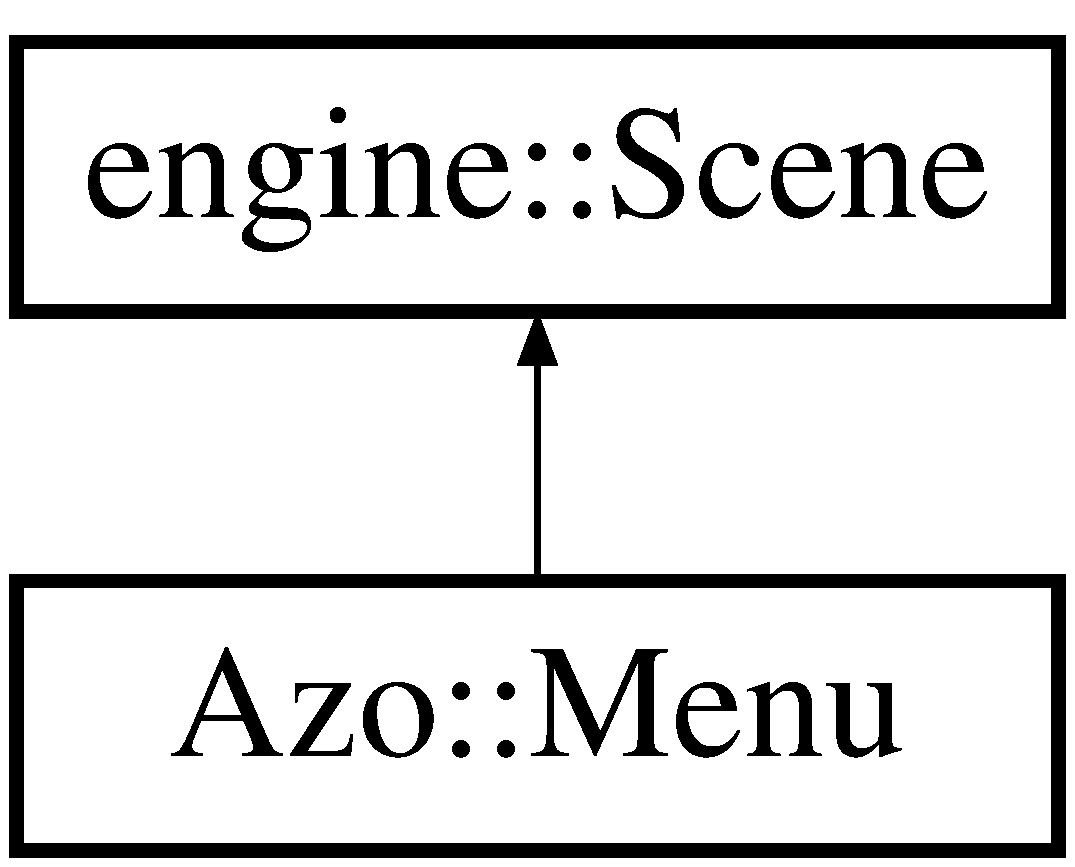
\includegraphics[height=2.000000cm]{class_azo_1_1_menu}
\end{center}
\end{figure}
\subsection*{Public Member Functions}
\begin{DoxyCompactItemize}
\item 
\hyperlink{class_azo_1_1_menu_ab688f65761b8e8f37d855cbca00fae2e}{Menu} ()
\item 
\hyperlink{class_azo_1_1_menu_a5b8be0abc6a6c078e5deeab8e2ef5d47}{Menu} (std\+::string name)
\begin{DoxyCompactList}\small\item\em function responsible for creating menu scene \end{DoxyCompactList}\item 
void \hyperlink{class_azo_1_1_menu_a7f375c556043d9e1964c670fc6d0d846}{restart} ()
\begin{DoxyCompactList}\small\item\em function responsible for restarting the game \end{DoxyCompactList}\item 
void \hyperlink{class_azo_1_1_menu_a999a8b12f7d1e6572c65f1a97cb3163a}{shutdown} ()
\begin{DoxyCompactList}\small\item\em function responsible for debugging \end{DoxyCompactList}\end{DoxyCompactItemize}
\subsection*{Additional Inherited Members}


\subsection{Detailed Description}
A Hitbox class. \hyperlink{class_azo_1_1_menu}{Menu} class. 

A more elaborate class description. Class responsible for creating the \textquotesingle{} menu \textquotesingle{} 

Definition at line 25 of file menu.\+hpp.



\subsection{Constructor \& Destructor Documentation}
\index{Azo\+::\+Menu@{Azo\+::\+Menu}!Menu@{Menu}}
\index{Menu@{Menu}!Azo\+::\+Menu@{Azo\+::\+Menu}}
\subsubsection[{\texorpdfstring{Menu()}{Menu()}}]{\setlength{\rightskip}{0pt plus 5cm}Azo\+::\+Menu\+::\+Menu (
\begin{DoxyParamCaption}
{}
\end{DoxyParamCaption}
)}\hypertarget{class_azo_1_1_menu_ab688f65761b8e8f37d855cbca00fae2e}{}\label{class_azo_1_1_menu_ab688f65761b8e8f37d855cbca00fae2e}
\index{Azo\+::\+Menu@{Azo\+::\+Menu}!Menu@{Menu}}
\index{Menu@{Menu}!Azo\+::\+Menu@{Azo\+::\+Menu}}
\subsubsection[{\texorpdfstring{Menu(std\+::string name)}{Menu(std::string name)}}]{\setlength{\rightskip}{0pt plus 5cm}Menu\+::\+Menu (
\begin{DoxyParamCaption}
\item[{std\+::string}]{name}
\end{DoxyParamCaption}
)}\hypertarget{class_azo_1_1_menu_a5b8be0abc6a6c078e5deeab8e2ef5d47}{}\label{class_azo_1_1_menu_a5b8be0abc6a6c078e5deeab8e2ef5d47}


function responsible for creating menu scene 


\begin{DoxyItemize}
\item T11 Why\+: Because it is necessary for the player to have access to the game menu before it starts 
\end{DoxyItemize}

Definition at line 19 of file menu.\+cpp.



\subsection{Member Function Documentation}
\index{Azo\+::\+Menu@{Azo\+::\+Menu}!restart@{restart}}
\index{restart@{restart}!Azo\+::\+Menu@{Azo\+::\+Menu}}
\subsubsection[{\texorpdfstring{restart()}{restart()}}]{\setlength{\rightskip}{0pt plus 5cm}void Menu\+::restart (
\begin{DoxyParamCaption}
{}
\end{DoxyParamCaption}
)\hspace{0.3cm}{\ttfamily [virtual]}}\hypertarget{class_azo_1_1_menu_a7f375c556043d9e1964c670fc6d0d846}{}\label{class_azo_1_1_menu_a7f375c556043d9e1964c670fc6d0d846}


function responsible for restarting the game 


\begin{DoxyItemize}
\item T11 Why\+: Because it is necessary that the player can restart the game

\begin{DoxyReturn}{Returns}
\char`\"{}void\char`\"{}. 
\end{DoxyReturn}

\end{DoxyItemize}

Reimplemented from \hyperlink{classengine_1_1_scene_a279192188f7c239355209afd3e7c16ac}{engine\+::\+Scene}.



Definition at line 31 of file menu.\+cpp.

\index{Azo\+::\+Menu@{Azo\+::\+Menu}!shutdown@{shutdown}}
\index{shutdown@{shutdown}!Azo\+::\+Menu@{Azo\+::\+Menu}}
\subsubsection[{\texorpdfstring{shutdown()}{shutdown()}}]{\setlength{\rightskip}{0pt plus 5cm}void Menu\+::shutdown (
\begin{DoxyParamCaption}
{}
\end{DoxyParamCaption}
)\hspace{0.3cm}{\ttfamily [virtual]}}\hypertarget{class_azo_1_1_menu_a999a8b12f7d1e6572c65f1a97cb3163a}{}\label{class_azo_1_1_menu_a999a8b12f7d1e6572c65f1a97cb3163a}


function responsible for debugging 


\begin{DoxyItemize}
\item T11 Why\+: Because it is responsible for debugging the code

\begin{DoxyReturn}{Returns}
\char`\"{}void\char`\"{}. 
\end{DoxyReturn}

\end{DoxyItemize}

Reimplemented from \hyperlink{classengine_1_1_scene_afdc5c5539730b162ddb6fd99b0c0660c}{engine\+::\+Scene}.



Definition at line 224 of file menu.\+cpp.



The documentation for this class was generated from the following files\+:\begin{DoxyCompactItemize}
\item 
include/\hyperlink{menu_8hpp}{menu.\+hpp}\item 
src/\hyperlink{menu_8cpp}{menu.\+cpp}\end{DoxyCompactItemize}

\hypertarget{class_azo_1_1_menu_code}{}\section{Azo\+:\+:Menu\+Code Class Reference}
\label{class_azo_1_1_menu_code}\index{Azo\+::\+Menu\+Code@{Azo\+::\+Menu\+Code}}


A Hitbox class. \hyperlink{class_azo_1_1_menu_code}{Menu\+Code} class.  




{\ttfamily \#include $<$menu\+\_\+code.\+hpp$>$}

Inheritance diagram for Azo\+:\+:Menu\+Code\+:\begin{figure}[H]
\begin{center}
\leavevmode
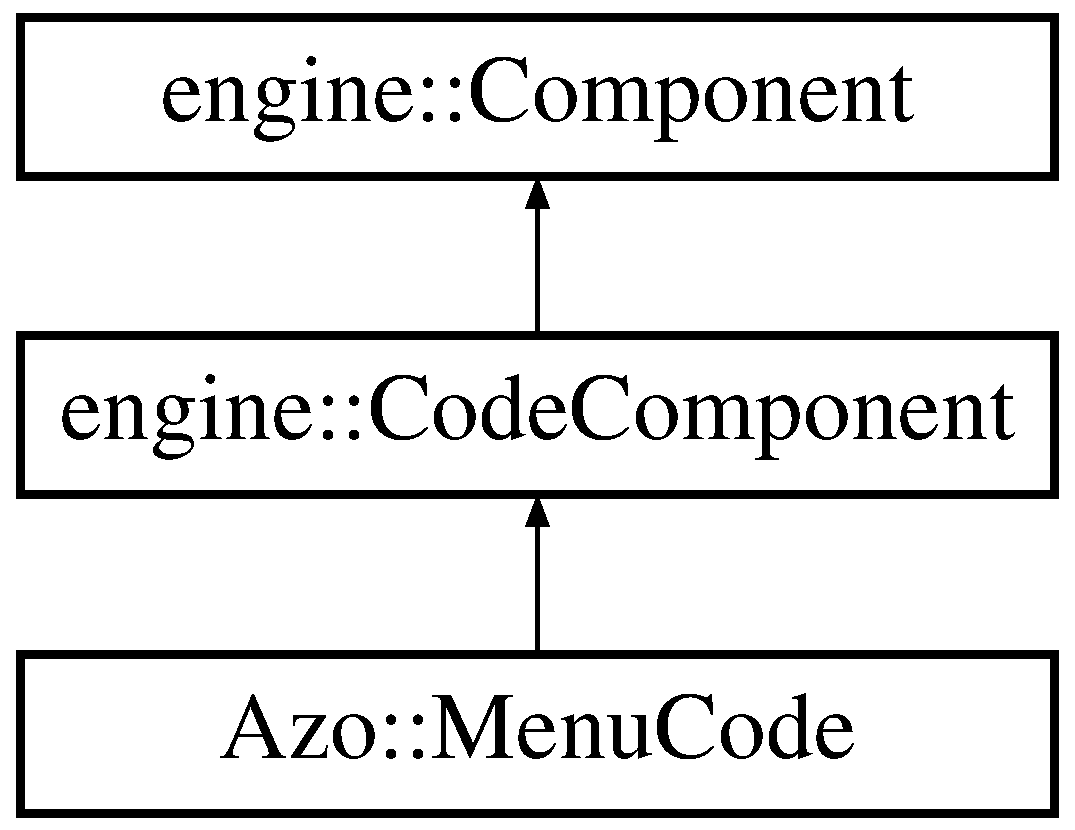
\includegraphics[height=3.000000cm]{class_azo_1_1_menu_code}
\end{center}
\end{figure}
\subsection*{Public Member Functions}
\begin{DoxyCompactItemize}
\item 
\hyperlink{class_azo_1_1_menu_code_a97efbd5b0b0e65a1c5adb823aa978e08}{Menu\+Code} (\hyperlink{classengine_1_1_game_object}{engine\+::\+Game\+Object} $\ast$\hyperlink{classengine_1_1_component_ad4a4865ca4df98ebea34d04a4ec5ad07}{game\+Object})
\begin{DoxyCompactList}\small\item\em function responsible for building menu \end{DoxyCompactList}\end{DoxyCompactItemize}
\subsection*{Additional Inherited Members}


\subsection{Detailed Description}
A Hitbox class. \hyperlink{class_azo_1_1_menu_code}{Menu\+Code} class. 

A more elaborate class description. Class responsible for creating the \hyperlink{class_azo_1_1_menu}{Menu} features 

Definition at line 24 of file menu\+\_\+code.\+hpp.



\subsection{Constructor \& Destructor Documentation}
\index{Azo\+::\+Menu\+Code@{Azo\+::\+Menu\+Code}!Menu\+Code@{Menu\+Code}}
\index{Menu\+Code@{Menu\+Code}!Azo\+::\+Menu\+Code@{Azo\+::\+Menu\+Code}}
\subsubsection[{\texorpdfstring{Menu\+Code(engine\+::\+Game\+Object $\ast$game\+Object)}{MenuCode(engine::GameObject *gameObject)}}]{\setlength{\rightskip}{0pt plus 5cm}Menu\+Code\+::\+Menu\+Code (
\begin{DoxyParamCaption}
\item[{{\bf engine\+::\+Game\+Object} $\ast$}]{game\+Object}
\end{DoxyParamCaption}
)}\hypertarget{class_azo_1_1_menu_code_a97efbd5b0b0e65a1c5adb823aa978e08}{}\label{class_azo_1_1_menu_code_a97efbd5b0b0e65a1c5adb823aa978e08}


function responsible for building menu 

Why\+: Used to build menu on the map


\begin{DoxyParams}{Parameters}
{\em Gameobject} & that is the creation object of the \textquotesingle{} menu \textquotesingle{} \\
\hline
\end{DoxyParams}


Definition at line 22 of file menu\+\_\+code.\+cpp.



The documentation for this class was generated from the following files\+:\begin{DoxyCompactItemize}
\item 
include/\hyperlink{menu__code_8hpp}{menu\+\_\+code.\+hpp}\item 
src/\hyperlink{menu__code_8cpp}{menu\+\_\+code.\+cpp}\end{DoxyCompactItemize}

\hypertarget{class_azo_1_1_obstacle}{}\section{Azo\+:\+:Obstacle Class Reference}
\label{class_azo_1_1_obstacle}\index{Azo\+::\+Obstacle@{Azo\+::\+Obstacle}}


\hyperlink{class_azo_1_1_obstacle}{Obstacle} class for in-\/game objects with collision.  




{\ttfamily \#include $<$obstacle.\+hpp$>$}

Inheritance diagram for Azo\+:\+:Obstacle\+:\begin{figure}[H]
\begin{center}
\leavevmode
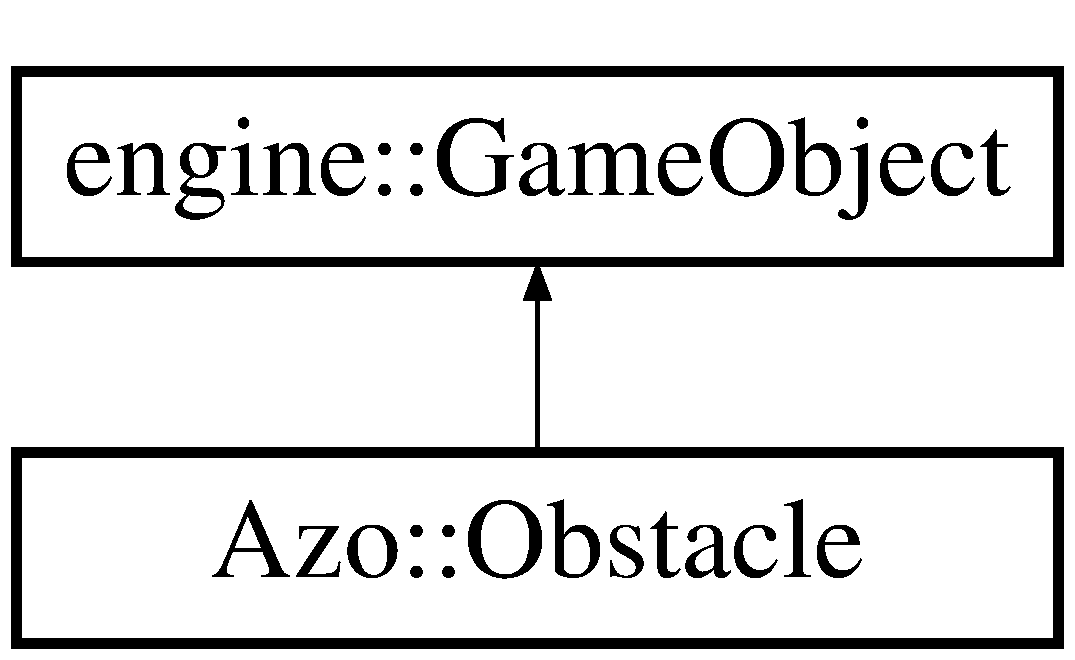
\includegraphics[height=2.000000cm]{class_azo_1_1_obstacle}
\end{center}
\end{figure}
\subsection*{Public Member Functions}
\begin{DoxyCompactItemize}
\item 
\hyperlink{class_azo_1_1_obstacle_a8f734072321fa06a7b7dae2d5f50f352}{Obstacle} ()
\begin{DoxyCompactList}\small\item\em Basic contructor for \hyperlink{class_azo_1_1_obstacle}{Obstacle}. \end{DoxyCompactList}\item 
virtual \hyperlink{class_azo_1_1_obstacle_af2f9cc9c6cff75dca0974fd5ac4f71a9}{$\sim$\+Obstacle} ()
\begin{DoxyCompactList}\small\item\em Virtual constructor for \hyperlink{class_azo_1_1_obstacle}{Obstacle}. \end{DoxyCompactList}\item 
\hyperlink{class_azo_1_1_obstacle_ac2605eab1c4049885e27749fe8bd4b14}{Obstacle} (std\+::string name, std\+::pair$<$ double, double $>$ position\+Relative\+To\+Parent, \hyperlink{namespace_azo_ac4ec77a26f64a5b7cd450e40dad04059}{Obstacle\+Type} obstacle\+Type)
\begin{DoxyCompactList}\small\item\em Constructor class for \hyperlink{class_azo_1_1_obstacle}{Obstacle}. \end{DoxyCompactList}\item 
void \hyperlink{class_azo_1_1_obstacle_aaff76ad6fd2803f73e941446e1724674}{shutdown} ()
\begin{DoxyCompactList}\small\item\em Destructor class for \hyperlink{class_azo_1_1_obstacle}{Obstacle}. \end{DoxyCompactList}\item 
std\+::string \hyperlink{class_azo_1_1_obstacle_a376685ade60d5c05661ce0bceab19da6}{get\+Class\+Name} ()
\begin{DoxyCompactList}\small\item\em Method for class name. \end{DoxyCompactList}\end{DoxyCompactItemize}
\subsection*{Public Attributes}
\begin{DoxyCompactItemize}
\item 
std\+::pair$<$ double, double $>$ \hyperlink{class_azo_1_1_obstacle_aac3846345bf1ae1070d8b407fb4f7c3a}{m\+Position\+Relative\+To\+Parent}
\item 
std\+::list$<$ \hyperlink{class_azo_1_1_invisible_block}{Invisible\+Block} $\ast$ $>$ \hyperlink{class_azo_1_1_obstacle_a535374cbd0b83f289b0644eda7650e48}{m\+Block\+List}
\item 
\hyperlink{namespace_azo_ac4ec77a26f64a5b7cd450e40dad04059}{Obstacle\+Type} \hyperlink{class_azo_1_1_obstacle_aaab3518ffd0b5360643383a9199e7e7d}{m\+Obstacle\+Type}
\item 
\hyperlink{namespace_azo_a75e30005795a46482a25b996ca785c67}{Machine\+Part\+State} \hyperlink{class_azo_1_1_obstacle_a3408445f79b6339fc2b72cd1d98676a4}{m\+Machine\+Part\+State} = \hyperlink{namespace_azo_a75e30005795a46482a25b996ca785c67a66b3c5ed1d52d8dcffab16270f632960}{Machine\+Part\+State\+::\+N\+O\+N\+\_\+\+M\+A\+C\+H\+I\+NE}
\end{DoxyCompactItemize}
\subsection*{Additional Inherited Members}


\subsection{Detailed Description}
\hyperlink{class_azo_1_1_obstacle}{Obstacle} class for in-\/game objects with collision. 

Used to create game objects that the player has to avoid in order to progress or has to collect in-\/game(such as Machine\+Parts). 

Definition at line 57 of file obstacle.\+hpp.



\subsection{Constructor \& Destructor Documentation}
\index{Azo\+::\+Obstacle@{Azo\+::\+Obstacle}!Obstacle@{Obstacle}}
\index{Obstacle@{Obstacle}!Azo\+::\+Obstacle@{Azo\+::\+Obstacle}}
\subsubsection[{\texorpdfstring{Obstacle()}{Obstacle()}}]{\setlength{\rightskip}{0pt plus 5cm}Obstacle\+::\+Obstacle (
\begin{DoxyParamCaption}
{}
\end{DoxyParamCaption}
)}\hypertarget{class_azo_1_1_obstacle_a8f734072321fa06a7b7dae2d5f50f352}{}\label{class_azo_1_1_obstacle_a8f734072321fa06a7b7dae2d5f50f352}


Basic contructor for \hyperlink{class_azo_1_1_obstacle}{Obstacle}. 

Default basic constructor for \hyperlink{class_azo_1_1_obstacle}{Obstacle}. 

Definition at line 19 of file obstacle.\+cpp.

\index{Azo\+::\+Obstacle@{Azo\+::\+Obstacle}!````~Obstacle@{$\sim$\+Obstacle}}
\index{````~Obstacle@{$\sim$\+Obstacle}!Azo\+::\+Obstacle@{Azo\+::\+Obstacle}}
\subsubsection[{\texorpdfstring{$\sim$\+Obstacle()}{~Obstacle()}}]{\setlength{\rightskip}{0pt plus 5cm}Obstacle\+::$\sim$\+Obstacle (
\begin{DoxyParamCaption}
{}
\end{DoxyParamCaption}
)\hspace{0.3cm}{\ttfamily [virtual]}}\hypertarget{class_azo_1_1_obstacle_af2f9cc9c6cff75dca0974fd5ac4f71a9}{}\label{class_azo_1_1_obstacle_af2f9cc9c6cff75dca0974fd5ac4f71a9}


Virtual constructor for \hyperlink{class_azo_1_1_obstacle}{Obstacle}. 

Default virtual constructor for \hyperlink{class_azo_1_1_obstacle}{Obstacle}. 

Definition at line 26 of file obstacle.\+cpp.

\index{Azo\+::\+Obstacle@{Azo\+::\+Obstacle}!Obstacle@{Obstacle}}
\index{Obstacle@{Obstacle}!Azo\+::\+Obstacle@{Azo\+::\+Obstacle}}
\subsubsection[{\texorpdfstring{Obstacle(std\+::string name, std\+::pair$<$ double, double $>$ position\+Relative\+To\+Parent, Obstacle\+Type obstacle\+Type)}{Obstacle(std::string name, std::pair< double, double > positionRelativeToParent, ObstacleType obstacleType)}}]{\setlength{\rightskip}{0pt plus 5cm}Obstacle\+::\+Obstacle (
\begin{DoxyParamCaption}
\item[{std\+::string}]{name, }
\item[{std\+::pair$<$ double, double $>$}]{position\+Relative\+To\+Parent, }
\item[{{\bf Obstacle\+Type}}]{obstacle\+Type}
\end{DoxyParamCaption}
)}\hypertarget{class_azo_1_1_obstacle_ac2605eab1c4049885e27749fe8bd4b14}{}\label{class_azo_1_1_obstacle_ac2605eab1c4049885e27749fe8bd4b14}


Constructor class for \hyperlink{class_azo_1_1_obstacle}{Obstacle}. 

Used to initialize \hyperlink{class_azo_1_1_obstacle}{Obstacle} class variables. 
\begin{DoxyParams}{Parameters}
{\em name} & \hyperlink{class_azo_1_1_obstacle}{Obstacle} name. \\
\hline
{\em position\+Relative\+To\+Parent} & Pair of doubles relative to position(range $>$ 0). \\
\hline
{\em obstacle\+Type} & Type of obstacle according to enum class Obstacle\+Type from \hyperlink{obstacle_8hpp}{obstacle.\+hpp} . \\
\hline
\end{DoxyParams}


Definition at line 96 of file obstacle.\+cpp.



\subsection{Member Function Documentation}
\index{Azo\+::\+Obstacle@{Azo\+::\+Obstacle}!get\+Class\+Name@{get\+Class\+Name}}
\index{get\+Class\+Name@{get\+Class\+Name}!Azo\+::\+Obstacle@{Azo\+::\+Obstacle}}
\subsubsection[{\texorpdfstring{get\+Class\+Name()}{getClassName()}}]{\setlength{\rightskip}{0pt plus 5cm}std\+::string Azo\+::\+Obstacle\+::get\+Class\+Name (
\begin{DoxyParamCaption}
{}
\end{DoxyParamCaption}
)\hspace{0.3cm}{\ttfamily [inline]}, {\ttfamily [virtual]}}\hypertarget{class_azo_1_1_obstacle_a376685ade60d5c05661ce0bceab19da6}{}\label{class_azo_1_1_obstacle_a376685ade60d5c05661ce0bceab19da6}


Method for class name. 

Inline method for returning the class\textquotesingle{} name. 

Reimplemented from \hyperlink{classengine_1_1_game_object_ac836deb7933c725ac09b67386ad10239}{engine\+::\+Game\+Object}.



Definition at line 81 of file obstacle.\+hpp.

\index{Azo\+::\+Obstacle@{Azo\+::\+Obstacle}!shutdown@{shutdown}}
\index{shutdown@{shutdown}!Azo\+::\+Obstacle@{Azo\+::\+Obstacle}}
\subsubsection[{\texorpdfstring{shutdown()}{shutdown()}}]{\setlength{\rightskip}{0pt plus 5cm}void Obstacle\+::shutdown (
\begin{DoxyParamCaption}
{}
\end{DoxyParamCaption}
)\hspace{0.3cm}{\ttfamily [virtual]}}\hypertarget{class_azo_1_1_obstacle_aaff76ad6fd2803f73e941446e1724674}{}\label{class_azo_1_1_obstacle_aaff76ad6fd2803f73e941446e1724674}


Destructor class for \hyperlink{class_azo_1_1_obstacle}{Obstacle}. 

Used for shutting down each one of the \hyperlink{class_azo_1_1_obstacle}{Obstacle}\textquotesingle{}s attributes so as to free memory when closing the game. 

Reimplemented from \hyperlink{classengine_1_1_game_object_a08d7a48b6eb90f55c8b670b6f98ab393}{engine\+::\+Game\+Object}.



Definition at line 35 of file obstacle.\+cpp.



\subsection{Member Data Documentation}
\index{Azo\+::\+Obstacle@{Azo\+::\+Obstacle}!m\+Block\+List@{m\+Block\+List}}
\index{m\+Block\+List@{m\+Block\+List}!Azo\+::\+Obstacle@{Azo\+::\+Obstacle}}
\subsubsection[{\texorpdfstring{m\+Block\+List}{mBlockList}}]{\setlength{\rightskip}{0pt plus 5cm}std\+::list$<${\bf Invisible\+Block} $\ast$$>$ Azo\+::\+Obstacle\+::m\+Block\+List}\hypertarget{class_azo_1_1_obstacle_a535374cbd0b83f289b0644eda7650e48}{}\label{class_azo_1_1_obstacle_a535374cbd0b83f289b0644eda7650e48}


Definition at line 60 of file obstacle.\+hpp.

\index{Azo\+::\+Obstacle@{Azo\+::\+Obstacle}!m\+Machine\+Part\+State@{m\+Machine\+Part\+State}}
\index{m\+Machine\+Part\+State@{m\+Machine\+Part\+State}!Azo\+::\+Obstacle@{Azo\+::\+Obstacle}}
\subsubsection[{\texorpdfstring{m\+Machine\+Part\+State}{mMachinePartState}}]{\setlength{\rightskip}{0pt plus 5cm}{\bf Machine\+Part\+State} Azo\+::\+Obstacle\+::m\+Machine\+Part\+State = {\bf Machine\+Part\+State\+::\+N\+O\+N\+\_\+\+M\+A\+C\+H\+I\+NE}}\hypertarget{class_azo_1_1_obstacle_a3408445f79b6339fc2b72cd1d98676a4}{}\label{class_azo_1_1_obstacle_a3408445f79b6339fc2b72cd1d98676a4}


Definition at line 62 of file obstacle.\+hpp.

\index{Azo\+::\+Obstacle@{Azo\+::\+Obstacle}!m\+Obstacle\+Type@{m\+Obstacle\+Type}}
\index{m\+Obstacle\+Type@{m\+Obstacle\+Type}!Azo\+::\+Obstacle@{Azo\+::\+Obstacle}}
\subsubsection[{\texorpdfstring{m\+Obstacle\+Type}{mObstacleType}}]{\setlength{\rightskip}{0pt plus 5cm}{\bf Obstacle\+Type} Azo\+::\+Obstacle\+::m\+Obstacle\+Type}\hypertarget{class_azo_1_1_obstacle_aaab3518ffd0b5360643383a9199e7e7d}{}\label{class_azo_1_1_obstacle_aaab3518ffd0b5360643383a9199e7e7d}


Definition at line 61 of file obstacle.\+hpp.

\index{Azo\+::\+Obstacle@{Azo\+::\+Obstacle}!m\+Position\+Relative\+To\+Parent@{m\+Position\+Relative\+To\+Parent}}
\index{m\+Position\+Relative\+To\+Parent@{m\+Position\+Relative\+To\+Parent}!Azo\+::\+Obstacle@{Azo\+::\+Obstacle}}
\subsubsection[{\texorpdfstring{m\+Position\+Relative\+To\+Parent}{mPositionRelativeToParent}}]{\setlength{\rightskip}{0pt plus 5cm}std\+::pair$<$double, double$>$ Azo\+::\+Obstacle\+::m\+Position\+Relative\+To\+Parent}\hypertarget{class_azo_1_1_obstacle_aac3846345bf1ae1070d8b407fb4f7c3a}{}\label{class_azo_1_1_obstacle_aac3846345bf1ae1070d8b407fb4f7c3a}


Definition at line 59 of file obstacle.\+hpp.



The documentation for this class was generated from the following files\+:\begin{DoxyCompactItemize}
\item 
include/\hyperlink{obstacle_8hpp}{obstacle.\+hpp}\item 
src/\hyperlink{obstacle_8cpp}{obstacle.\+cpp}\end{DoxyCompactItemize}

\hypertarget{class_azo_1_1_player}{}\section{Azo\+:\+:Player Class Reference}
\label{class_azo_1_1_player}\index{Azo\+::\+Player@{Azo\+::\+Player}}


\hyperlink{class_azo_1_1_player}{Player} class This class is used to characterize player and set its configurations and behaviour.  




{\ttfamily \#include $<$player.\+hpp$>$}

Inheritance diagram for Azo\+:\+:Player\+:\begin{figure}[H]
\begin{center}
\leavevmode
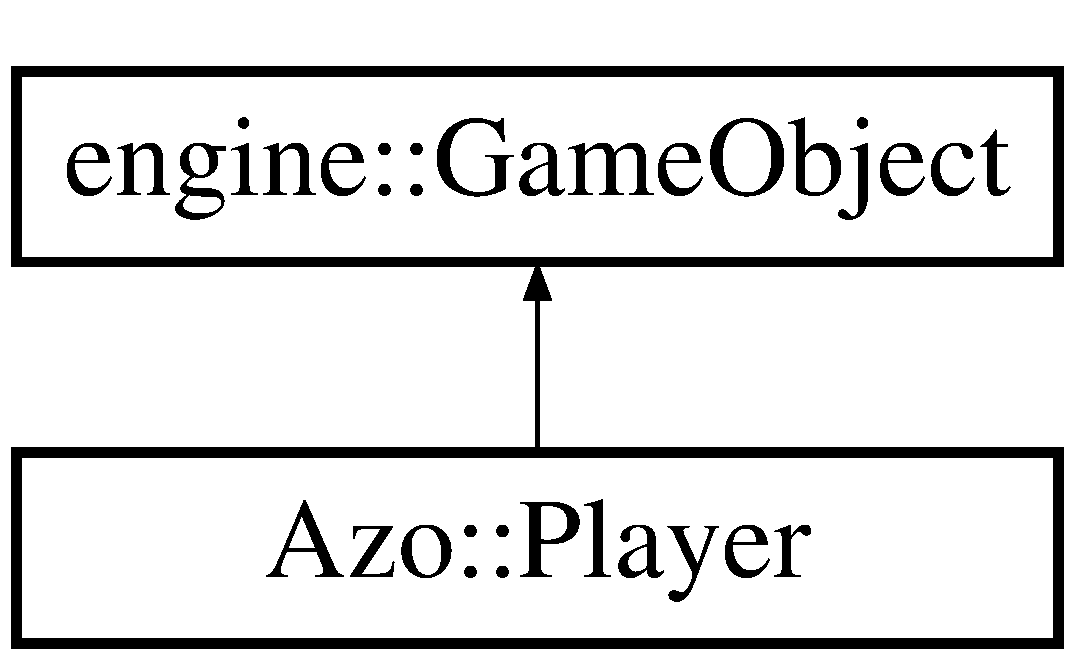
\includegraphics[height=2.000000cm]{class_azo_1_1_player}
\end{center}
\end{figure}
\subsection*{Public Member Functions}
\begin{DoxyCompactItemize}
\item 
\hyperlink{class_azo_1_1_player_a70594f977b11b9574450b1f4510f6ee5}{Player} ()
\item 
\hyperlink{class_azo_1_1_player_a4e229f75d3c2e31f502ca0bb48f6a42f}{Player} (std\+::string name, std\+::pair$<$ double, double $>$ current\+Position)
\item 
void \hyperlink{class_azo_1_1_player_a57070d462aa21dbfb8dc645b2a25bf86}{shutdown} ()
\begin{DoxyCompactList}\small\item\em inherits function that disable the game components. \end{DoxyCompactList}\end{DoxyCompactItemize}
\subsection*{Public Attributes}
\begin{DoxyCompactItemize}
\item 
const std\+::pair$<$ double, double $>$ \hyperlink{class_azo_1_1_player_a7c56f1e510b86c4719bef956b69befa4}{M\+\_\+\+Z\+E\+R\+O\+\_\+\+V\+E\+C\+T\+OR} = std\+::make\+\_\+pair(0.\+0f, 0.\+0f)
\item 
const double \hyperlink{class_azo_1_1_player_a2daa546daa4c5f15640d703fdde56059}{M\+\_\+\+G\+R\+A\+V\+I\+TY} = 0.\+003f
\item 
const double \hyperlink{class_azo_1_1_player_a926fea900dde401f4b2b5faa28bfa7c6}{M\+\_\+\+J\+U\+M\+P\+I\+N\+G\+\_\+\+S\+P\+E\+ED} = -\/1.\+0f
\item 
const double \hyperlink{class_azo_1_1_player_a597ac6977889f5bef7f95aaf13ff3f85}{M\+\_\+\+W\+A\+L\+K\+I\+N\+G\+\_\+\+S\+P\+E\+ED} = 4.\+8f
\item 
const int \hyperlink{class_azo_1_1_player_a4cd316a415fb0af5d4179a6cd32a2ab2}{M\+\_\+\+T\+O\+T\+A\+L\+\_\+\+P\+A\+R\+TS} = 25
\item 
\hyperlink{namespace_azo_ab6013e2aec3a179604cef5ea80418e33}{Player\+State} \hyperlink{class_azo_1_1_player_a6c500f32806b1450aaf2acb66ae5b9bf}{m\+State}
\item 
std\+::pair$<$ double, double $>$ \hyperlink{class_azo_1_1_player_a545f3a8fe6ace68bc67f9573ba179b3b}{m\+Speed}
\item 
bool \hyperlink{class_azo_1_1_player_a777f7f3207c772734e886188c85523fe}{m\+Pushes\+Right\+Wall}
\item 
bool \hyperlink{class_azo_1_1_player_a49cc98a0198d753b53837cdd6d35539d}{m\+Pushes\+Left\+Wall}
\item 
bool \hyperlink{class_azo_1_1_player_a3bd316a4da8a7b1da0b9844a3d6b1e49}{m\+At\+Ceiling}
\item 
bool \hyperlink{class_azo_1_1_player_af525a6da7698c344f378ece79dcd28bc}{m\+On\+Ground}
\item 
int \hyperlink{class_azo_1_1_player_a7d2a2c8e92e8fd22aa1dc220fd6d6df7}{m\+Collected\+Parts} = 0
\end{DoxyCompactItemize}
\subsection*{Additional Inherited Members}


\subsection{Detailed Description}
\hyperlink{class_azo_1_1_player}{Player} class This class is used to characterize player and set its configurations and behaviour. 

Definition at line 46 of file player.\+hpp.



\subsection{Constructor \& Destructor Documentation}
\index{Azo\+::\+Player@{Azo\+::\+Player}!Player@{Player}}
\index{Player@{Player}!Azo\+::\+Player@{Azo\+::\+Player}}
\subsubsection[{\texorpdfstring{Player()}{Player()}}]{\setlength{\rightskip}{0pt plus 5cm}Azo\+::\+Player\+::\+Player (
\begin{DoxyParamCaption}
{}
\end{DoxyParamCaption}
)}\hypertarget{class_azo_1_1_player_a70594f977b11b9574450b1f4510f6ee5}{}\label{class_azo_1_1_player_a70594f977b11b9574450b1f4510f6ee5}
\index{Azo\+::\+Player@{Azo\+::\+Player}!Player@{Player}}
\index{Player@{Player}!Azo\+::\+Player@{Azo\+::\+Player}}
\subsubsection[{\texorpdfstring{Player(std\+::string name, std\+::pair$<$ double, double $>$ current\+Position)}{Player(std::string name, std::pair< double, double > currentPosition)}}]{\setlength{\rightskip}{0pt plus 5cm}Player\+::\+Player (
\begin{DoxyParamCaption}
\item[{std\+::string}]{name, }
\item[{std\+::pair$<$ double, double $>$}]{current\+Position}
\end{DoxyParamCaption}
)}\hypertarget{class_azo_1_1_player_a4e229f75d3c2e31f502ca0bb48f6a42f}{}\label{class_azo_1_1_player_a4e229f75d3c2e31f502ca0bb48f6a42f}


Definition at line 20 of file player.\+cpp.



\subsection{Member Function Documentation}
\index{Azo\+::\+Player@{Azo\+::\+Player}!shutdown@{shutdown}}
\index{shutdown@{shutdown}!Azo\+::\+Player@{Azo\+::\+Player}}
\subsubsection[{\texorpdfstring{shutdown()}{shutdown()}}]{\setlength{\rightskip}{0pt plus 5cm}void Player\+::shutdown (
\begin{DoxyParamCaption}
{}
\end{DoxyParamCaption}
)\hspace{0.3cm}{\ttfamily [virtual]}}\hypertarget{class_azo_1_1_player_a57070d462aa21dbfb8dc645b2a25bf86}{}\label{class_azo_1_1_player_a57070d462aa21dbfb8dc645b2a25bf86}


inherits function that disable the game components. 

free the component pointers.

\begin{DoxyReturn}{Returns}
\char`\"{}void\char`\"{}. 
\end{DoxyReturn}


Reimplemented from \hyperlink{classengine_1_1_game_object_a08d7a48b6eb90f55c8b670b6f98ab393}{engine\+::\+Game\+Object}.



Definition at line 30 of file player.\+cpp.



\subsection{Member Data Documentation}
\index{Azo\+::\+Player@{Azo\+::\+Player}!M\+\_\+\+G\+R\+A\+V\+I\+TY@{M\+\_\+\+G\+R\+A\+V\+I\+TY}}
\index{M\+\_\+\+G\+R\+A\+V\+I\+TY@{M\+\_\+\+G\+R\+A\+V\+I\+TY}!Azo\+::\+Player@{Azo\+::\+Player}}
\subsubsection[{\texorpdfstring{M\+\_\+\+G\+R\+A\+V\+I\+TY}{M_GRAVITY}}]{\setlength{\rightskip}{0pt plus 5cm}const double Azo\+::\+Player\+::\+M\+\_\+\+G\+R\+A\+V\+I\+TY = 0.\+003f}\hypertarget{class_azo_1_1_player_a2daa546daa4c5f15640d703fdde56059}{}\label{class_azo_1_1_player_a2daa546daa4c5f15640d703fdde56059}


Definition at line 76 of file player.\+hpp.

\index{Azo\+::\+Player@{Azo\+::\+Player}!M\+\_\+\+J\+U\+M\+P\+I\+N\+G\+\_\+\+S\+P\+E\+ED@{M\+\_\+\+J\+U\+M\+P\+I\+N\+G\+\_\+\+S\+P\+E\+ED}}
\index{M\+\_\+\+J\+U\+M\+P\+I\+N\+G\+\_\+\+S\+P\+E\+ED@{M\+\_\+\+J\+U\+M\+P\+I\+N\+G\+\_\+\+S\+P\+E\+ED}!Azo\+::\+Player@{Azo\+::\+Player}}
\subsubsection[{\texorpdfstring{M\+\_\+\+J\+U\+M\+P\+I\+N\+G\+\_\+\+S\+P\+E\+ED}{M_JUMPING_SPEED}}]{\setlength{\rightskip}{0pt plus 5cm}const double Azo\+::\+Player\+::\+M\+\_\+\+J\+U\+M\+P\+I\+N\+G\+\_\+\+S\+P\+E\+ED = -\/1.\+0f}\hypertarget{class_azo_1_1_player_a926fea900dde401f4b2b5faa28bfa7c6}{}\label{class_azo_1_1_player_a926fea900dde401f4b2b5faa28bfa7c6}


Definition at line 77 of file player.\+hpp.

\index{Azo\+::\+Player@{Azo\+::\+Player}!M\+\_\+\+T\+O\+T\+A\+L\+\_\+\+P\+A\+R\+TS@{M\+\_\+\+T\+O\+T\+A\+L\+\_\+\+P\+A\+R\+TS}}
\index{M\+\_\+\+T\+O\+T\+A\+L\+\_\+\+P\+A\+R\+TS@{M\+\_\+\+T\+O\+T\+A\+L\+\_\+\+P\+A\+R\+TS}!Azo\+::\+Player@{Azo\+::\+Player}}
\subsubsection[{\texorpdfstring{M\+\_\+\+T\+O\+T\+A\+L\+\_\+\+P\+A\+R\+TS}{M_TOTAL_PARTS}}]{\setlength{\rightskip}{0pt plus 5cm}const int Azo\+::\+Player\+::\+M\+\_\+\+T\+O\+T\+A\+L\+\_\+\+P\+A\+R\+TS = 25}\hypertarget{class_azo_1_1_player_a4cd316a415fb0af5d4179a6cd32a2ab2}{}\label{class_azo_1_1_player_a4cd316a415fb0af5d4179a6cd32a2ab2}


Definition at line 80 of file player.\+hpp.

\index{Azo\+::\+Player@{Azo\+::\+Player}!M\+\_\+\+W\+A\+L\+K\+I\+N\+G\+\_\+\+S\+P\+E\+ED@{M\+\_\+\+W\+A\+L\+K\+I\+N\+G\+\_\+\+S\+P\+E\+ED}}
\index{M\+\_\+\+W\+A\+L\+K\+I\+N\+G\+\_\+\+S\+P\+E\+ED@{M\+\_\+\+W\+A\+L\+K\+I\+N\+G\+\_\+\+S\+P\+E\+ED}!Azo\+::\+Player@{Azo\+::\+Player}}
\subsubsection[{\texorpdfstring{M\+\_\+\+W\+A\+L\+K\+I\+N\+G\+\_\+\+S\+P\+E\+ED}{M_WALKING_SPEED}}]{\setlength{\rightskip}{0pt plus 5cm}const double Azo\+::\+Player\+::\+M\+\_\+\+W\+A\+L\+K\+I\+N\+G\+\_\+\+S\+P\+E\+ED = 4.\+8f}\hypertarget{class_azo_1_1_player_a597ac6977889f5bef7f95aaf13ff3f85}{}\label{class_azo_1_1_player_a597ac6977889f5bef7f95aaf13ff3f85}


Definition at line 79 of file player.\+hpp.

\index{Azo\+::\+Player@{Azo\+::\+Player}!M\+\_\+\+Z\+E\+R\+O\+\_\+\+V\+E\+C\+T\+OR@{M\+\_\+\+Z\+E\+R\+O\+\_\+\+V\+E\+C\+T\+OR}}
\index{M\+\_\+\+Z\+E\+R\+O\+\_\+\+V\+E\+C\+T\+OR@{M\+\_\+\+Z\+E\+R\+O\+\_\+\+V\+E\+C\+T\+OR}!Azo\+::\+Player@{Azo\+::\+Player}}
\subsubsection[{\texorpdfstring{M\+\_\+\+Z\+E\+R\+O\+\_\+\+V\+E\+C\+T\+OR}{M_ZERO_VECTOR}}]{\setlength{\rightskip}{0pt plus 5cm}const std\+::pair$<$double, double$>$ Azo\+::\+Player\+::\+M\+\_\+\+Z\+E\+R\+O\+\_\+\+V\+E\+C\+T\+OR = std\+::make\+\_\+pair(0.\+0f, 0.\+0f)}\hypertarget{class_azo_1_1_player_a7c56f1e510b86c4719bef956b69befa4}{}\label{class_azo_1_1_player_a7c56f1e510b86c4719bef956b69befa4}


Definition at line 75 of file player.\+hpp.

\index{Azo\+::\+Player@{Azo\+::\+Player}!m\+At\+Ceiling@{m\+At\+Ceiling}}
\index{m\+At\+Ceiling@{m\+At\+Ceiling}!Azo\+::\+Player@{Azo\+::\+Player}}
\subsubsection[{\texorpdfstring{m\+At\+Ceiling}{mAtCeiling}}]{\setlength{\rightskip}{0pt plus 5cm}bool Azo\+::\+Player\+::m\+At\+Ceiling}\hypertarget{class_azo_1_1_player_a3bd316a4da8a7b1da0b9844a3d6b1e49}{}\label{class_azo_1_1_player_a3bd316a4da8a7b1da0b9844a3d6b1e49}


Definition at line 87 of file player.\+hpp.

\index{Azo\+::\+Player@{Azo\+::\+Player}!m\+Collected\+Parts@{m\+Collected\+Parts}}
\index{m\+Collected\+Parts@{m\+Collected\+Parts}!Azo\+::\+Player@{Azo\+::\+Player}}
\subsubsection[{\texorpdfstring{m\+Collected\+Parts}{mCollectedParts}}]{\setlength{\rightskip}{0pt plus 5cm}int Azo\+::\+Player\+::m\+Collected\+Parts = 0}\hypertarget{class_azo_1_1_player_a7d2a2c8e92e8fd22aa1dc220fd6d6df7}{}\label{class_azo_1_1_player_a7d2a2c8e92e8fd22aa1dc220fd6d6df7}


Definition at line 90 of file player.\+hpp.

\index{Azo\+::\+Player@{Azo\+::\+Player}!m\+On\+Ground@{m\+On\+Ground}}
\index{m\+On\+Ground@{m\+On\+Ground}!Azo\+::\+Player@{Azo\+::\+Player}}
\subsubsection[{\texorpdfstring{m\+On\+Ground}{mOnGround}}]{\setlength{\rightskip}{0pt plus 5cm}bool Azo\+::\+Player\+::m\+On\+Ground}\hypertarget{class_azo_1_1_player_af525a6da7698c344f378ece79dcd28bc}{}\label{class_azo_1_1_player_af525a6da7698c344f378ece79dcd28bc}


Definition at line 88 of file player.\+hpp.

\index{Azo\+::\+Player@{Azo\+::\+Player}!m\+Pushes\+Left\+Wall@{m\+Pushes\+Left\+Wall}}
\index{m\+Pushes\+Left\+Wall@{m\+Pushes\+Left\+Wall}!Azo\+::\+Player@{Azo\+::\+Player}}
\subsubsection[{\texorpdfstring{m\+Pushes\+Left\+Wall}{mPushesLeftWall}}]{\setlength{\rightskip}{0pt plus 5cm}bool Azo\+::\+Player\+::m\+Pushes\+Left\+Wall}\hypertarget{class_azo_1_1_player_a49cc98a0198d753b53837cdd6d35539d}{}\label{class_azo_1_1_player_a49cc98a0198d753b53837cdd6d35539d}


Definition at line 86 of file player.\+hpp.

\index{Azo\+::\+Player@{Azo\+::\+Player}!m\+Pushes\+Right\+Wall@{m\+Pushes\+Right\+Wall}}
\index{m\+Pushes\+Right\+Wall@{m\+Pushes\+Right\+Wall}!Azo\+::\+Player@{Azo\+::\+Player}}
\subsubsection[{\texorpdfstring{m\+Pushes\+Right\+Wall}{mPushesRightWall}}]{\setlength{\rightskip}{0pt plus 5cm}bool Azo\+::\+Player\+::m\+Pushes\+Right\+Wall}\hypertarget{class_azo_1_1_player_a777f7f3207c772734e886188c85523fe}{}\label{class_azo_1_1_player_a777f7f3207c772734e886188c85523fe}


Definition at line 85 of file player.\+hpp.

\index{Azo\+::\+Player@{Azo\+::\+Player}!m\+Speed@{m\+Speed}}
\index{m\+Speed@{m\+Speed}!Azo\+::\+Player@{Azo\+::\+Player}}
\subsubsection[{\texorpdfstring{m\+Speed}{mSpeed}}]{\setlength{\rightskip}{0pt plus 5cm}std\+::pair$<$double, double$>$ Azo\+::\+Player\+::m\+Speed}\hypertarget{class_azo_1_1_player_a545f3a8fe6ace68bc67f9573ba179b3b}{}\label{class_azo_1_1_player_a545f3a8fe6ace68bc67f9573ba179b3b}


Definition at line 83 of file player.\+hpp.

\index{Azo\+::\+Player@{Azo\+::\+Player}!m\+State@{m\+State}}
\index{m\+State@{m\+State}!Azo\+::\+Player@{Azo\+::\+Player}}
\subsubsection[{\texorpdfstring{m\+State}{mState}}]{\setlength{\rightskip}{0pt plus 5cm}{\bf Player\+State} Azo\+::\+Player\+::m\+State}\hypertarget{class_azo_1_1_player_a6c500f32806b1450aaf2acb66ae5b9bf}{}\label{class_azo_1_1_player_a6c500f32806b1450aaf2acb66ae5b9bf}


Definition at line 82 of file player.\+hpp.



The documentation for this class was generated from the following files\+:\begin{DoxyCompactItemize}
\item 
include/\hyperlink{player_8hpp}{player.\+hpp}\item 
src/\hyperlink{player_8cpp}{player.\+cpp}\end{DoxyCompactItemize}

\hypertarget{class_azo_1_1_player_code}{}\section{Azo\+:\+:Player\+Code Class Reference}
\label{class_azo_1_1_player_code}\index{Azo\+::\+Player\+Code@{Azo\+::\+Player\+Code}}


\hyperlink{class_azo_1_1_player_code}{Player\+Code} class This class is used to controll the player\textquotesingle{}s character behaviour. It updates player\textquotesingle{}s animation and audios according to the events.  




{\ttfamily \#include $<$player\+\_\+code.\+hpp$>$}

Inheritance diagram for Azo\+:\+:Player\+Code\+:\begin{figure}[H]
\begin{center}
\leavevmode
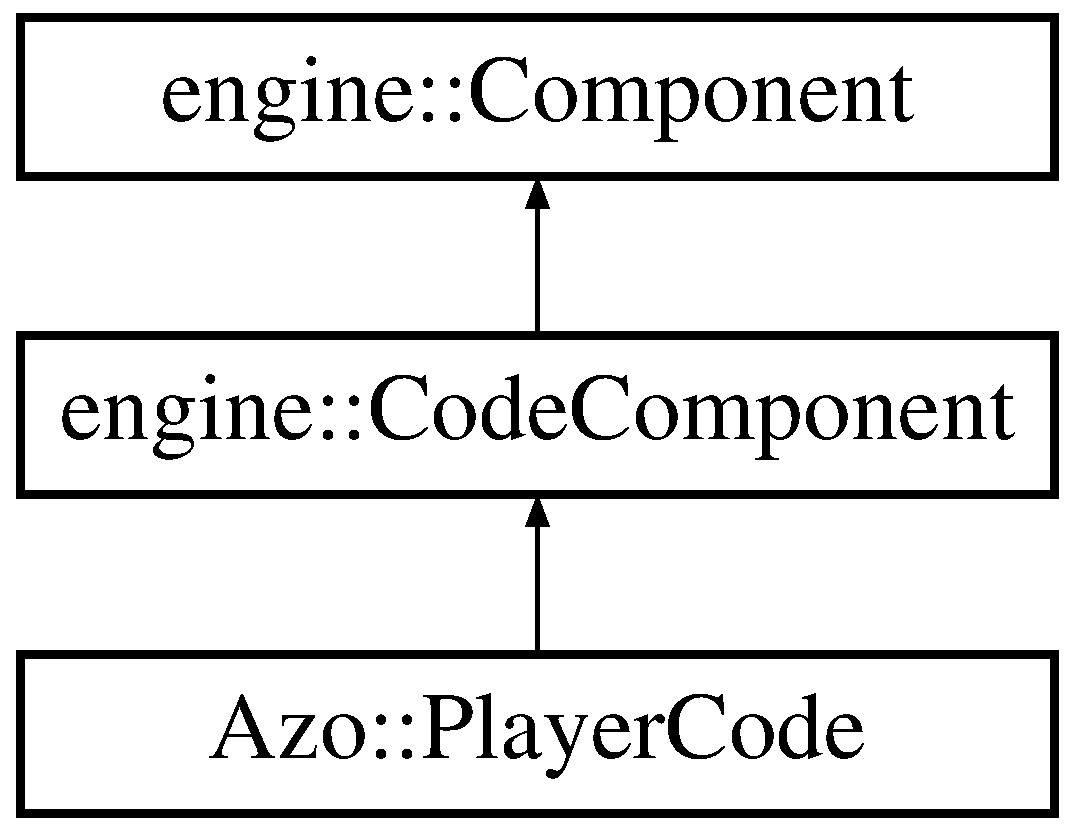
\includegraphics[height=3.000000cm]{class_azo_1_1_player_code}
\end{center}
\end{figure}
\subsection*{Public Member Functions}
\begin{DoxyCompactItemize}
\item 
\hyperlink{class_azo_1_1_player_code_a8f40c27c0a16f344eb324321f6b3bd58}{Player\+Code} ()
\begin{DoxyCompactList}\small\item\em default constructor for \hyperlink{class_azo_1_1_player_code}{Player\+Code} Object \end{DoxyCompactList}\item 
virtual \hyperlink{class_azo_1_1_player_code_af59a02bc37b40f8f2b89c2c840105094}{$\sim$\+Player\+Code} ()
\begin{DoxyCompactList}\small\item\em default destructor for \hyperlink{class_azo_1_1_player_code}{Player\+Code} Object \end{DoxyCompactList}\item 
\hyperlink{class_azo_1_1_player_code_a9952382660834549c2fcd2fafb32a20b}{Player\+Code} (\hyperlink{class_azo_1_1_player}{Player} $\ast$player)
\begin{DoxyCompactList}\small\item\em overwritten constructor for the \hyperlink{class_azo_1_1_player_code}{Player\+Code} object. \end{DoxyCompactList}\item 
void \hyperlink{class_azo_1_1_player_code_aea1004e3e9f7c7c58d69f428dd0b5b6f}{shutdown} ()
\begin{DoxyCompactList}\small\item\em free the animation pointer when charcter dies, free the animation pointer \end{DoxyCompactList}\end{DoxyCompactItemize}
\subsection*{Additional Inherited Members}


\subsection{Detailed Description}
\hyperlink{class_azo_1_1_player_code}{Player\+Code} class This class is used to controll the player\textquotesingle{}s character behaviour. It updates player\textquotesingle{}s animation and audios according to the events. 

Definition at line 29 of file player\+\_\+code.\+hpp.



\subsection{Constructor \& Destructor Documentation}
\index{Azo\+::\+Player\+Code@{Azo\+::\+Player\+Code}!Player\+Code@{Player\+Code}}
\index{Player\+Code@{Player\+Code}!Azo\+::\+Player\+Code@{Azo\+::\+Player\+Code}}
\subsubsection[{\texorpdfstring{Player\+Code()}{PlayerCode()}}]{\setlength{\rightskip}{0pt plus 5cm}Player\+Code\+::\+Player\+Code (
\begin{DoxyParamCaption}
{}
\end{DoxyParamCaption}
)}\hypertarget{class_azo_1_1_player_code_a8f40c27c0a16f344eb324321f6b3bd58}{}\label{class_azo_1_1_player_code_a8f40c27c0a16f344eb324321f6b3bd58}


default constructor for \hyperlink{class_azo_1_1_player_code}{Player\+Code} Object 

\begin{DoxyReturn}{Returns}
\char`\"{}void\char`\"{}. 
\end{DoxyReturn}


Definition at line 26 of file player\+\_\+code.\+cpp.

\index{Azo\+::\+Player\+Code@{Azo\+::\+Player\+Code}!````~Player\+Code@{$\sim$\+Player\+Code}}
\index{````~Player\+Code@{$\sim$\+Player\+Code}!Azo\+::\+Player\+Code@{Azo\+::\+Player\+Code}}
\subsubsection[{\texorpdfstring{$\sim$\+Player\+Code()}{~PlayerCode()}}]{\setlength{\rightskip}{0pt plus 5cm}Player\+Code\+::$\sim$\+Player\+Code (
\begin{DoxyParamCaption}
{}
\end{DoxyParamCaption}
)\hspace{0.3cm}{\ttfamily [virtual]}}\hypertarget{class_azo_1_1_player_code_af59a02bc37b40f8f2b89c2c840105094}{}\label{class_azo_1_1_player_code_af59a02bc37b40f8f2b89c2c840105094}


default destructor for \hyperlink{class_azo_1_1_player_code}{Player\+Code} Object 

\begin{DoxyReturn}{Returns}
\char`\"{}void\char`\"{}. 
\end{DoxyReturn}


Definition at line 33 of file player\+\_\+code.\+cpp.

\index{Azo\+::\+Player\+Code@{Azo\+::\+Player\+Code}!Player\+Code@{Player\+Code}}
\index{Player\+Code@{Player\+Code}!Azo\+::\+Player\+Code@{Azo\+::\+Player\+Code}}
\subsubsection[{\texorpdfstring{Player\+Code(\+Player $\ast$player)}{PlayerCode(Player *player)}}]{\setlength{\rightskip}{0pt plus 5cm}Player\+Code\+::\+Player\+Code (
\begin{DoxyParamCaption}
\item[{{\bf Player} $\ast$}]{player}
\end{DoxyParamCaption}
)}\hypertarget{class_azo_1_1_player_code_a9952382660834549c2fcd2fafb32a20b}{}\label{class_azo_1_1_player_code_a9952382660834549c2fcd2fafb32a20b}


overwritten constructor for the \hyperlink{class_azo_1_1_player_code}{Player\+Code} object. 


\begin{DoxyParams}{Parameters}
{\em pointer} & reffering to player \\
\hline
\end{DoxyParams}
\begin{DoxyReturn}{Returns}
\char`\"{}void\char`\"{}. 
\end{DoxyReturn}


Definition at line 41 of file player\+\_\+code.\+cpp.



\subsection{Member Function Documentation}
\index{Azo\+::\+Player\+Code@{Azo\+::\+Player\+Code}!shutdown@{shutdown}}
\index{shutdown@{shutdown}!Azo\+::\+Player\+Code@{Azo\+::\+Player\+Code}}
\subsubsection[{\texorpdfstring{shutdown()}{shutdown()}}]{\setlength{\rightskip}{0pt plus 5cm}void Player\+Code\+::shutdown (
\begin{DoxyParamCaption}
{}
\end{DoxyParamCaption}
)\hspace{0.3cm}{\ttfamily [virtual]}}\hypertarget{class_azo_1_1_player_code_aea1004e3e9f7c7c58d69f428dd0b5b6f}{}\label{class_azo_1_1_player_code_aea1004e3e9f7c7c58d69f428dd0b5b6f}


free the animation pointer when charcter dies, free the animation pointer 

\begin{DoxyReturn}{Returns}
\textquotesingle{}void\textquotesingle{}. 
\end{DoxyReturn}


Reimplemented from \hyperlink{classengine_1_1_code_component_af76ba17f9f87216418081d1e2c7c3a22}{engine\+::\+Code\+Component}.



Definition at line 75 of file player\+\_\+code.\+cpp.



The documentation for this class was generated from the following files\+:\begin{DoxyCompactItemize}
\item 
include/\hyperlink{player__code_8hpp}{player\+\_\+code.\+hpp}\item 
src/\hyperlink{player__code_8cpp}{player\+\_\+code.\+cpp}\end{DoxyCompactItemize}

\hypertarget{classengine_1_1_scene}{}\section{engine\+:\+:Scene Class Reference}
\label{classengine_1_1_scene}\index{engine\+::\+Scene@{engine\+::\+Scene}}


{\ttfamily \#include $<$scene.\+hpp$>$}

Inheritance diagram for engine\+:\+:Scene\+:\begin{figure}[H]
\begin{center}
\leavevmode
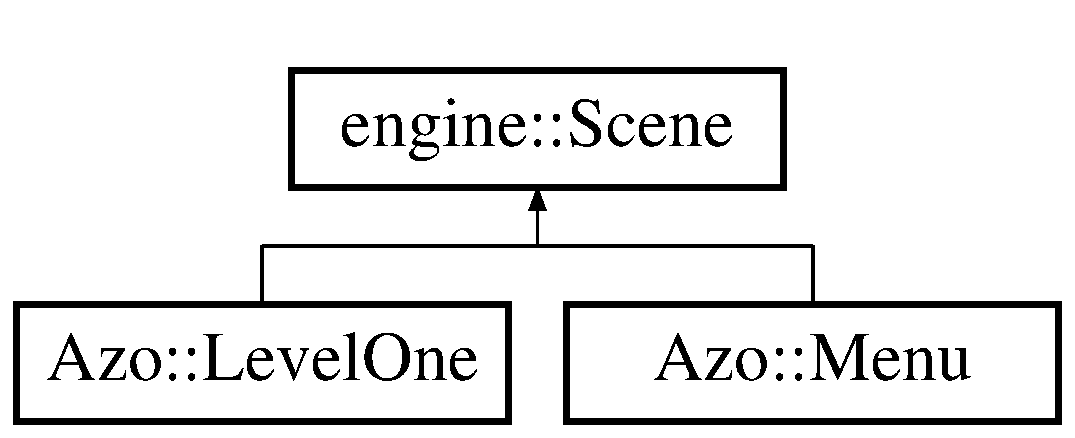
\includegraphics[height=2.000000cm]{classengine_1_1_scene}
\end{center}
\end{figure}
\subsection*{Public Member Functions}
\begin{DoxyCompactItemize}
\item 
\hyperlink{classengine_1_1_scene_ad10176d75a9cc0da56626f682d083507}{Scene} ()
\item 
\hyperlink{classengine_1_1_scene_a06cf49594fe578fbcd662ab0e976cbd5}{Scene} (std\+::string \hyperlink{classengine_1_1_scene_a62943c09d12941bc32feab48e2d7d38a}{scene\+Name})
\item 
virtual void \hyperlink{classengine_1_1_scene_abb3b6efc6fdba03cd96436edaf08a967}{init} ()
\item 
virtual void \hyperlink{classengine_1_1_scene_afdc5c5539730b162ddb6fd99b0c0660c}{shutdown} ()
\item 
virtual void \hyperlink{classengine_1_1_scene_ac0e3d2c98ba6063a086467fb2c19142f}{draw} ()
\item 
virtual void \hyperlink{classengine_1_1_scene_ab8eb8334aee22d2797aedbacef9e3874}{update\+Code} ()
\item 
virtual void \hyperlink{classengine_1_1_scene_a279192188f7c239355209afd3e7c16ac}{restart} ()
\item 
std\+::string \hyperlink{classengine_1_1_scene_a4e9388d63f1576d127928a91d00fe8c8}{get\+Scene\+Name} ()
\item 
void \hyperlink{classengine_1_1_scene_a1035f4628a4878a0f1a7eb4082b83ded}{delete\+Key\+List} ()
\item 
void \hyperlink{classengine_1_1_scene_a2c1e265823a5e281e1970377674f0ff9}{add\+Game\+Object} (\hyperlink{classengine_1_1_game_object}{engine\+::\+Game\+Object} \&game\+Object)
\item 
void \hyperlink{classengine_1_1_scene_a02bb6e553349fe8a37f58cfe1bbc93cf}{remove\+Game\+Object} (std\+::string \&game\+Object\+Name)
\item 
\hyperlink{classengine_1_1_game_object}{engine\+::\+Game\+Object} \& \hyperlink{classengine_1_1_scene_af8eacc131836e089cd14f7b1ca88484c}{get\+Game\+Object} (std\+::string \&game\+Object\+Name)
\end{DoxyCompactItemize}
\subsection*{Public Attributes}
\begin{DoxyCompactItemize}
\item 
\hyperlink{namespaceengine_a49a8e8541d5f387918f566b7909abd98}{Scene\+State} \hyperlink{classengine_1_1_scene_a25912176ae12eab48035b7d218955466}{m\+State} = \hyperlink{namespaceengine_a49a8e8541d5f387918f566b7909abd98a7f6c43f1f96a930f7d49210196a52ad2}{Scene\+State\+::\+F\+I\+R\+S\+T\+\_\+\+T\+I\+ME}
\end{DoxyCompactItemize}
\subsection*{Protected Attributes}
\begin{DoxyCompactItemize}
\item 
std\+::map$<$ std\+::string, \hyperlink{classengine_1_1_game_object}{engine\+::\+Game\+Object} $\ast$ $>$ \hyperlink{classengine_1_1_scene_a7b27b00796602fc52515114b17f06ea4}{game\+Object\+Map}
\item 
std\+::list$<$ std\+::string $>$ \hyperlink{classengine_1_1_scene_a1fff54180b377adb5d66dc75e6494d5e}{m\+Key\+List}
\item 
std\+::string \hyperlink{classengine_1_1_scene_a62943c09d12941bc32feab48e2d7d38a}{scene\+Name}
\end{DoxyCompactItemize}


\subsection{Detailed Description}


Definition at line 35 of file scene.\+hpp.



\subsection{Constructor \& Destructor Documentation}
\index{engine\+::\+Scene@{engine\+::\+Scene}!Scene@{Scene}}
\index{Scene@{Scene}!engine\+::\+Scene@{engine\+::\+Scene}}
\subsubsection[{\texorpdfstring{Scene()}{Scene()}}]{\setlength{\rightskip}{0pt plus 5cm}Scene\+::\+Scene (
\begin{DoxyParamCaption}
{}
\end{DoxyParamCaption}
)}\hypertarget{classengine_1_1_scene_ad10176d75a9cc0da56626f682d083507}{}\label{classengine_1_1_scene_ad10176d75a9cc0da56626f682d083507}


Definition at line 14 of file scene.\+cpp.

\index{engine\+::\+Scene@{engine\+::\+Scene}!Scene@{Scene}}
\index{Scene@{Scene}!engine\+::\+Scene@{engine\+::\+Scene}}
\subsubsection[{\texorpdfstring{Scene(std\+::string scene\+Name)}{Scene(std::string sceneName)}}]{\setlength{\rightskip}{0pt plus 5cm}Scene\+::\+Scene (
\begin{DoxyParamCaption}
\item[{std\+::string}]{scene\+Name}
\end{DoxyParamCaption}
)}\hypertarget{classengine_1_1_scene_a06cf49594fe578fbcd662ab0e976cbd5}{}\label{classengine_1_1_scene_a06cf49594fe578fbcd662ab0e976cbd5}


Definition at line 21 of file scene.\+cpp.



\subsection{Member Function Documentation}
\index{engine\+::\+Scene@{engine\+::\+Scene}!add\+Game\+Object@{add\+Game\+Object}}
\index{add\+Game\+Object@{add\+Game\+Object}!engine\+::\+Scene@{engine\+::\+Scene}}
\subsubsection[{\texorpdfstring{add\+Game\+Object(engine\+::\+Game\+Object \&game\+Object)}{addGameObject(engine::GameObject &gameObject)}}]{\setlength{\rightskip}{0pt plus 5cm}void Scene\+::add\+Game\+Object (
\begin{DoxyParamCaption}
\item[{{\bf engine\+::\+Game\+Object} \&}]{game\+Object}
\end{DoxyParamCaption}
)}\hypertarget{classengine_1_1_scene_a2c1e265823a5e281e1970377674f0ff9}{}\label{classengine_1_1_scene_a2c1e265823a5e281e1970377674f0ff9}


Definition at line 94 of file scene.\+cpp.

\index{engine\+::\+Scene@{engine\+::\+Scene}!delete\+Key\+List@{delete\+Key\+List}}
\index{delete\+Key\+List@{delete\+Key\+List}!engine\+::\+Scene@{engine\+::\+Scene}}
\subsubsection[{\texorpdfstring{delete\+Key\+List()}{deleteKeyList()}}]{\setlength{\rightskip}{0pt plus 5cm}void Scene\+::delete\+Key\+List (
\begin{DoxyParamCaption}
{}
\end{DoxyParamCaption}
)}\hypertarget{classengine_1_1_scene_a1035f4628a4878a0f1a7eb4082b83ded}{}\label{classengine_1_1_scene_a1035f4628a4878a0f1a7eb4082b83ded}


Definition at line 52 of file scene.\+cpp.

\index{engine\+::\+Scene@{engine\+::\+Scene}!draw@{draw}}
\index{draw@{draw}!engine\+::\+Scene@{engine\+::\+Scene}}
\subsubsection[{\texorpdfstring{draw()}{draw()}}]{\setlength{\rightskip}{0pt plus 5cm}void Scene\+::draw (
\begin{DoxyParamCaption}
{}
\end{DoxyParamCaption}
)\hspace{0.3cm}{\ttfamily [virtual]}}\hypertarget{classengine_1_1_scene_ac0e3d2c98ba6063a086467fb2c19142f}{}\label{classengine_1_1_scene_ac0e3d2c98ba6063a086467fb2c19142f}


Definition at line 61 of file scene.\+cpp.

\index{engine\+::\+Scene@{engine\+::\+Scene}!get\+Game\+Object@{get\+Game\+Object}}
\index{get\+Game\+Object@{get\+Game\+Object}!engine\+::\+Scene@{engine\+::\+Scene}}
\subsubsection[{\texorpdfstring{get\+Game\+Object(std\+::string \&game\+Object\+Name)}{getGameObject(std::string &gameObjectName)}}]{\setlength{\rightskip}{0pt plus 5cm}{\bf Game\+Object} \& Scene\+::get\+Game\+Object (
\begin{DoxyParamCaption}
\item[{std\+::string \&}]{game\+Object\+Name}
\end{DoxyParamCaption}
)}\hypertarget{classengine_1_1_scene_af8eacc131836e089cd14f7b1ca88484c}{}\label{classengine_1_1_scene_af8eacc131836e089cd14f7b1ca88484c}


Definition at line 110 of file scene.\+cpp.

\index{engine\+::\+Scene@{engine\+::\+Scene}!get\+Scene\+Name@{get\+Scene\+Name}}
\index{get\+Scene\+Name@{get\+Scene\+Name}!engine\+::\+Scene@{engine\+::\+Scene}}
\subsubsection[{\texorpdfstring{get\+Scene\+Name()}{getSceneName()}}]{\setlength{\rightskip}{0pt plus 5cm}std\+::string engine\+::\+Scene\+::get\+Scene\+Name (
\begin{DoxyParamCaption}
{}
\end{DoxyParamCaption}
)\hspace{0.3cm}{\ttfamily [inline]}}\hypertarget{classengine_1_1_scene_a4e9388d63f1576d127928a91d00fe8c8}{}\label{classengine_1_1_scene_a4e9388d63f1576d127928a91d00fe8c8}


Definition at line 46 of file scene.\+hpp.

\index{engine\+::\+Scene@{engine\+::\+Scene}!init@{init}}
\index{init@{init}!engine\+::\+Scene@{engine\+::\+Scene}}
\subsubsection[{\texorpdfstring{init()}{init()}}]{\setlength{\rightskip}{0pt plus 5cm}void Scene\+::init (
\begin{DoxyParamCaption}
{}
\end{DoxyParamCaption}
)\hspace{0.3cm}{\ttfamily [virtual]}}\hypertarget{classengine_1_1_scene_abb3b6efc6fdba03cd96436edaf08a967}{}\label{classengine_1_1_scene_abb3b6efc6fdba03cd96436edaf08a967}


Definition at line 30 of file scene.\+cpp.

\index{engine\+::\+Scene@{engine\+::\+Scene}!remove\+Game\+Object@{remove\+Game\+Object}}
\index{remove\+Game\+Object@{remove\+Game\+Object}!engine\+::\+Scene@{engine\+::\+Scene}}
\subsubsection[{\texorpdfstring{remove\+Game\+Object(std\+::string \&game\+Object\+Name)}{removeGameObject(std::string &gameObjectName)}}]{\setlength{\rightskip}{0pt plus 5cm}void Scene\+::remove\+Game\+Object (
\begin{DoxyParamCaption}
\item[{std\+::string \&}]{game\+Object\+Name}
\end{DoxyParamCaption}
)}\hypertarget{classengine_1_1_scene_a02bb6e553349fe8a37f58cfe1bbc93cf}{}\label{classengine_1_1_scene_a02bb6e553349fe8a37f58cfe1bbc93cf}


Definition at line 123 of file scene.\+cpp.

\index{engine\+::\+Scene@{engine\+::\+Scene}!restart@{restart}}
\index{restart@{restart}!engine\+::\+Scene@{engine\+::\+Scene}}
\subsubsection[{\texorpdfstring{restart()}{restart()}}]{\setlength{\rightskip}{0pt plus 5cm}void Scene\+::restart (
\begin{DoxyParamCaption}
{}
\end{DoxyParamCaption}
)\hspace{0.3cm}{\ttfamily [virtual]}}\hypertarget{classengine_1_1_scene_a279192188f7c239355209afd3e7c16ac}{}\label{classengine_1_1_scene_a279192188f7c239355209afd3e7c16ac}


Reimplemented in \hyperlink{class_azo_1_1_level_one_ac388145a996f6663e2ae757f026f07f1}{Azo\+::\+Level\+One}, and \hyperlink{class_azo_1_1_menu_a7f375c556043d9e1964c670fc6d0d846}{Azo\+::\+Menu}.



Definition at line 87 of file scene.\+cpp.

\index{engine\+::\+Scene@{engine\+::\+Scene}!shutdown@{shutdown}}
\index{shutdown@{shutdown}!engine\+::\+Scene@{engine\+::\+Scene}}
\subsubsection[{\texorpdfstring{shutdown()}{shutdown()}}]{\setlength{\rightskip}{0pt plus 5cm}void Scene\+::shutdown (
\begin{DoxyParamCaption}
{}
\end{DoxyParamCaption}
)\hspace{0.3cm}{\ttfamily [virtual]}}\hypertarget{classengine_1_1_scene_afdc5c5539730b162ddb6fd99b0c0660c}{}\label{classengine_1_1_scene_afdc5c5539730b162ddb6fd99b0c0660c}


Reimplemented in \hyperlink{class_azo_1_1_menu_a999a8b12f7d1e6572c65f1a97cb3163a}{Azo\+::\+Menu}.



Definition at line 41 of file scene.\+cpp.

\index{engine\+::\+Scene@{engine\+::\+Scene}!update\+Code@{update\+Code}}
\index{update\+Code@{update\+Code}!engine\+::\+Scene@{engine\+::\+Scene}}
\subsubsection[{\texorpdfstring{update\+Code()}{updateCode()}}]{\setlength{\rightskip}{0pt plus 5cm}void Scene\+::update\+Code (
\begin{DoxyParamCaption}
{}
\end{DoxyParamCaption}
)\hspace{0.3cm}{\ttfamily [virtual]}}\hypertarget{classengine_1_1_scene_ab8eb8334aee22d2797aedbacef9e3874}{}\label{classengine_1_1_scene_ab8eb8334aee22d2797aedbacef9e3874}


Definition at line 74 of file scene.\+cpp.



\subsection{Member Data Documentation}
\index{engine\+::\+Scene@{engine\+::\+Scene}!game\+Object\+Map@{game\+Object\+Map}}
\index{game\+Object\+Map@{game\+Object\+Map}!engine\+::\+Scene@{engine\+::\+Scene}}
\subsubsection[{\texorpdfstring{game\+Object\+Map}{gameObjectMap}}]{\setlength{\rightskip}{0pt plus 5cm}std\+::map$<$std\+::string, {\bf engine\+::\+Game\+Object} $\ast$$>$ engine\+::\+Scene\+::game\+Object\+Map\hspace{0.3cm}{\ttfamily [protected]}}\hypertarget{classengine_1_1_scene_a7b27b00796602fc52515114b17f06ea4}{}\label{classengine_1_1_scene_a7b27b00796602fc52515114b17f06ea4}


Definition at line 57 of file scene.\+hpp.

\index{engine\+::\+Scene@{engine\+::\+Scene}!m\+Key\+List@{m\+Key\+List}}
\index{m\+Key\+List@{m\+Key\+List}!engine\+::\+Scene@{engine\+::\+Scene}}
\subsubsection[{\texorpdfstring{m\+Key\+List}{mKeyList}}]{\setlength{\rightskip}{0pt plus 5cm}std\+::list$<$std\+::string$>$ engine\+::\+Scene\+::m\+Key\+List\hspace{0.3cm}{\ttfamily [protected]}}\hypertarget{classengine_1_1_scene_a1fff54180b377adb5d66dc75e6494d5e}{}\label{classengine_1_1_scene_a1fff54180b377adb5d66dc75e6494d5e}


Definition at line 58 of file scene.\+hpp.

\index{engine\+::\+Scene@{engine\+::\+Scene}!m\+State@{m\+State}}
\index{m\+State@{m\+State}!engine\+::\+Scene@{engine\+::\+Scene}}
\subsubsection[{\texorpdfstring{m\+State}{mState}}]{\setlength{\rightskip}{0pt plus 5cm}{\bf Scene\+State} engine\+::\+Scene\+::m\+State = {\bf Scene\+State\+::\+F\+I\+R\+S\+T\+\_\+\+T\+I\+ME}}\hypertarget{classengine_1_1_scene_a25912176ae12eab48035b7d218955466}{}\label{classengine_1_1_scene_a25912176ae12eab48035b7d218955466}


Definition at line 54 of file scene.\+hpp.

\index{engine\+::\+Scene@{engine\+::\+Scene}!scene\+Name@{scene\+Name}}
\index{scene\+Name@{scene\+Name}!engine\+::\+Scene@{engine\+::\+Scene}}
\subsubsection[{\texorpdfstring{scene\+Name}{sceneName}}]{\setlength{\rightskip}{0pt plus 5cm}std\+::string engine\+::\+Scene\+::scene\+Name\hspace{0.3cm}{\ttfamily [protected]}}\hypertarget{classengine_1_1_scene_a62943c09d12941bc32feab48e2d7d38a}{}\label{classengine_1_1_scene_a62943c09d12941bc32feab48e2d7d38a}


Definition at line 59 of file scene.\+hpp.



The documentation for this class was generated from the following files\+:\begin{DoxyCompactItemize}
\item 
engine/include/\hyperlink{scene_8hpp}{scene.\+hpp}\item 
engine/src/\hyperlink{scene_8cpp}{scene.\+cpp}\end{DoxyCompactItemize}

\hypertarget{classengine_1_1_s_d_l}{}\section{engine\+:\+:S\+DL Class Reference}
\label{classengine_1_1_s_d_l}\index{engine\+::\+S\+DL@{engine\+::\+S\+DL}}


class that look after all \hyperlink{classengine_1_1_s_d_l}{S\+DL}\textquotesingle{}s dependences to run in first.  




{\ttfamily \#include $<$sdl.\+hpp$>$}

\subsection*{Public Member Functions}
\begin{DoxyCompactItemize}
\item 
\hyperlink{classengine_1_1_s_d_l_af3795554364a7fce185958eede6ad061}{S\+DL} ()
\begin{DoxyCompactList}\small\item\em Default constructor for the sdl. \end{DoxyCompactList}\item 
void \hyperlink{classengine_1_1_s_d_l_af6ee7dd9c220e82ce4f931a0325b315f}{set\+S\+D\+L\+Attributes} (std\+::string game\+Name, int window\+Width, int window\+Height)
\begin{DoxyCompactList}\small\item\em receive attributes of the \hyperlink{classengine_1_1_game}{Game} instance through \char`\"{}\+Set\+Game\+Attributes\char`\"{} method. \end{DoxyCompactList}\item 
void \hyperlink{classengine_1_1_s_d_l_a10afdc6fa827ad9c3772c7ef759a903c}{init\+S\+DL} ()
\begin{DoxyCompactList}\small\item\em initialize all \hyperlink{classengine_1_1_s_d_l}{S\+DL}. \end{DoxyCompactList}\item 
S\+D\+L\+\_\+\+Renderer $\ast$ \hyperlink{classengine_1_1_s_d_l_a3875fe564e0571ef84c899ead42675c6}{get\+Canvas} ()
\begin{DoxyCompactList}\small\item\em copy the code where the method is called. \end{DoxyCompactList}\item 
void \hyperlink{classengine_1_1_s_d_l_a3259aab79da90549924b0eb286e61e64}{create\+Window} ()
\begin{DoxyCompactList}\small\item\em creating the Window and Canvas. \end{DoxyCompactList}\item 
void \hyperlink{classengine_1_1_s_d_l_afcc094fe19573bc62d6a5c0537f6e073}{terminate\+S\+DL} ()
\begin{DoxyCompactList}\small\item\em terminating \hyperlink{classengine_1_1_s_d_l}{S\+DL}. \end{DoxyCompactList}\item 
int \hyperlink{classengine_1_1_s_d_l_a656bbafd95481b395aab1fdccef8a785}{get\+Window\+Width} ()
\begin{DoxyCompactList}\small\item\em private attribute \char`\"{}window\+\_\+width\char`\"{}. \end{DoxyCompactList}\item 
int \hyperlink{classengine_1_1_s_d_l_a4de4ede7cd92d53d0f509f2a2058e840}{get\+Window\+Height} ()
\begin{DoxyCompactList}\small\item\em private attribute \char`\"{}window\+\_\+height\char`\"{}. \end{DoxyCompactList}\end{DoxyCompactItemize}


\subsection{Detailed Description}
class that look after all \hyperlink{classengine_1_1_s_d_l}{S\+DL}\textquotesingle{}s dependences to run in first. 

Class that define the behavior of the sdl.

\begin{DoxyReturn}{Returns}
\char`\"{}void\char`\"{}. 
\end{DoxyReturn}


Definition at line 27 of file sdl.\+hpp.



\subsection{Constructor \& Destructor Documentation}
\index{engine\+::\+S\+DL@{engine\+::\+S\+DL}!S\+DL@{S\+DL}}
\index{S\+DL@{S\+DL}!engine\+::\+S\+DL@{engine\+::\+S\+DL}}
\subsubsection[{\texorpdfstring{S\+D\+L()}{SDL()}}]{\setlength{\rightskip}{0pt plus 5cm}S\+D\+L\+::\+S\+DL (
\begin{DoxyParamCaption}
{}
\end{DoxyParamCaption}
)}\hypertarget{classengine_1_1_s_d_l_af3795554364a7fce185958eede6ad061}{}\label{classengine_1_1_s_d_l_af3795554364a7fce185958eede6ad061}


Default constructor for the sdl. 

\begin{DoxyReturn}{Returns}
\char`\"{}void\char`\"{}. 
\end{DoxyReturn}


Definition at line 25 of file sdl.\+cpp.



\subsection{Member Function Documentation}
\index{engine\+::\+S\+DL@{engine\+::\+S\+DL}!create\+Window@{create\+Window}}
\index{create\+Window@{create\+Window}!engine\+::\+S\+DL@{engine\+::\+S\+DL}}
\subsubsection[{\texorpdfstring{create\+Window()}{createWindow()}}]{\setlength{\rightskip}{0pt plus 5cm}void S\+D\+L\+::create\+Window (
\begin{DoxyParamCaption}
{}
\end{DoxyParamCaption}
)}\hypertarget{classengine_1_1_s_d_l_a3259aab79da90549924b0eb286e61e64}{}\label{classengine_1_1_s_d_l_a3259aab79da90549924b0eb286e61e64}


creating the Window and Canvas. 

Used inside \char`\"{}\+Run\char`\"{} method of the \hyperlink{classengine_1_1_game}{Game}.

\begin{DoxyReturn}{Returns}
\char`\"{}void\char`\"{}. 
\end{DoxyReturn}


Definition at line 61 of file sdl.\+cpp.

\index{engine\+::\+S\+DL@{engine\+::\+S\+DL}!get\+Canvas@{get\+Canvas}}
\index{get\+Canvas@{get\+Canvas}!engine\+::\+S\+DL@{engine\+::\+S\+DL}}
\subsubsection[{\texorpdfstring{get\+Canvas()}{getCanvas()}}]{\setlength{\rightskip}{0pt plus 5cm}S\+D\+L\+\_\+\+Renderer$\ast$ engine\+::\+S\+D\+L\+::get\+Canvas (
\begin{DoxyParamCaption}
{}
\end{DoxyParamCaption}
)\hspace{0.3cm}{\ttfamily [inline]}}\hypertarget{classengine_1_1_s_d_l_a3875fe564e0571ef84c899ead42675c6}{}\label{classengine_1_1_s_d_l_a3875fe564e0571ef84c899ead42675c6}


copy the code where the method is called. 

Used to get Canvas with Inline to be more efficient.

\begin{DoxyReturn}{Returns}
\char`\"{}canvas\char`\"{}. 
\end{DoxyReturn}


Definition at line 60 of file sdl.\+hpp.

\index{engine\+::\+S\+DL@{engine\+::\+S\+DL}!get\+Window\+Height@{get\+Window\+Height}}
\index{get\+Window\+Height@{get\+Window\+Height}!engine\+::\+S\+DL@{engine\+::\+S\+DL}}
\subsubsection[{\texorpdfstring{get\+Window\+Height()}{getWindowHeight()}}]{\setlength{\rightskip}{0pt plus 5cm}int engine\+::\+S\+D\+L\+::get\+Window\+Height (
\begin{DoxyParamCaption}
{}
\end{DoxyParamCaption}
)\hspace{0.3cm}{\ttfamily [inline]}}\hypertarget{classengine_1_1_s_d_l_a4de4ede7cd92d53d0f509f2a2058e840}{}\label{classengine_1_1_s_d_l_a4de4ede7cd92d53d0f509f2a2058e840}


private attribute \char`\"{}window\+\_\+height\char`\"{}. 

Used to use the private attribute \char`\"{}window\+\_\+height\char`\"{}.

\begin{DoxyReturn}{Returns}
\char`\"{}window\+\_\+height\char`\"{}. 
\end{DoxyReturn}


Definition at line 102 of file sdl.\+hpp.

\index{engine\+::\+S\+DL@{engine\+::\+S\+DL}!get\+Window\+Width@{get\+Window\+Width}}
\index{get\+Window\+Width@{get\+Window\+Width}!engine\+::\+S\+DL@{engine\+::\+S\+DL}}
\subsubsection[{\texorpdfstring{get\+Window\+Width()}{getWindowWidth()}}]{\setlength{\rightskip}{0pt plus 5cm}int engine\+::\+S\+D\+L\+::get\+Window\+Width (
\begin{DoxyParamCaption}
{}
\end{DoxyParamCaption}
)\hspace{0.3cm}{\ttfamily [inline]}}\hypertarget{classengine_1_1_s_d_l_a656bbafd95481b395aab1fdccef8a785}{}\label{classengine_1_1_s_d_l_a656bbafd95481b395aab1fdccef8a785}


private attribute \char`\"{}window\+\_\+width\char`\"{}. 

Used to use the private attribute \char`\"{}window\+\_\+width\char`\"{}.

\begin{DoxyReturn}{Returns}
\char`\"{}window\+\_\+width\char`\"{}. 
\end{DoxyReturn}


Definition at line 90 of file sdl.\+hpp.

\index{engine\+::\+S\+DL@{engine\+::\+S\+DL}!init\+S\+DL@{init\+S\+DL}}
\index{init\+S\+DL@{init\+S\+DL}!engine\+::\+S\+DL@{engine\+::\+S\+DL}}
\subsubsection[{\texorpdfstring{init\+S\+D\+L()}{initSDL()}}]{\setlength{\rightskip}{0pt plus 5cm}void S\+D\+L\+::init\+S\+DL (
\begin{DoxyParamCaption}
{}
\end{DoxyParamCaption}
)}\hypertarget{classengine_1_1_s_d_l_a10afdc6fa827ad9c3772c7ef759a903c}{}\label{classengine_1_1_s_d_l_a10afdc6fa827ad9c3772c7ef759a903c}


initialize all \hyperlink{classengine_1_1_s_d_l}{S\+DL}. 

Initialize attributes to Windows, Canvas, S\+D\+L\+\_\+\+I\+M\+A\+GE, S\+D\+L\+\_\+\+V\+I\+D\+EO, S\+D\+L\+\_\+\+A\+U\+D\+IO.

\begin{DoxyReturn}{Returns}
\char`\"{}void\char`\"{}. 
\end{DoxyReturn}


Definition at line 34 of file sdl.\+cpp.

\index{engine\+::\+S\+DL@{engine\+::\+S\+DL}!set\+S\+D\+L\+Attributes@{set\+S\+D\+L\+Attributes}}
\index{set\+S\+D\+L\+Attributes@{set\+S\+D\+L\+Attributes}!engine\+::\+S\+DL@{engine\+::\+S\+DL}}
\subsubsection[{\texorpdfstring{set\+S\+D\+L\+Attributes(std\+::string game\+Name, int window\+Width, int window\+Height)}{setSDLAttributes(std::string gameName, int windowWidth, int windowHeight)}}]{\setlength{\rightskip}{0pt plus 5cm}void S\+D\+L\+::set\+S\+D\+L\+Attributes (
\begin{DoxyParamCaption}
\item[{std\+::string}]{game\+Name, }
\item[{int}]{window\+Width, }
\item[{int}]{window\+Height}
\end{DoxyParamCaption}
)}\hypertarget{classengine_1_1_s_d_l_af6ee7dd9c220e82ce4f931a0325b315f}{}\label{classengine_1_1_s_d_l_af6ee7dd9c220e82ce4f931a0325b315f}


receive attributes of the \hyperlink{classengine_1_1_game}{Game} instance through \char`\"{}\+Set\+Game\+Attributes\char`\"{} method. 

receive attributes of the \hyperlink{classengine_1_1_game}{Game} instance.

\begin{DoxyReturn}{Returns}
\char`\"{}void\char`\"{}.
\end{DoxyReturn}
Throught \char`\"{}\+Set\+Game\+Attributes\char`\"{} method.


\begin{DoxyParams}{Parameters}
{\em game\+Name} & string that says the name of the game. \\
\hline
{\em window\+Width} & integer that is responsible for the width of the window. \\
\hline
{\em window\+Heighth} & integer that is responsible for the heith of the window.\\
\hline
\end{DoxyParams}
\begin{DoxyReturn}{Returns}
\char`\"{}void\char`\"{}. 
\end{DoxyReturn}


Definition at line 136 of file sdl.\+cpp.

\index{engine\+::\+S\+DL@{engine\+::\+S\+DL}!terminate\+S\+DL@{terminate\+S\+DL}}
\index{terminate\+S\+DL@{terminate\+S\+DL}!engine\+::\+S\+DL@{engine\+::\+S\+DL}}
\subsubsection[{\texorpdfstring{terminate\+S\+D\+L()}{terminateSDL()}}]{\setlength{\rightskip}{0pt plus 5cm}void S\+D\+L\+::terminate\+S\+DL (
\begin{DoxyParamCaption}
{}
\end{DoxyParamCaption}
)}\hypertarget{classengine_1_1_s_d_l_afcc094fe19573bc62d6a5c0537f6e073}{}\label{classengine_1_1_s_d_l_afcc094fe19573bc62d6a5c0537f6e073}


terminating \hyperlink{classengine_1_1_s_d_l}{S\+DL}. 

Used in the Main Loop\textquotesingle{}s End.

\begin{DoxyReturn}{Returns}
\char`\"{}void\char`\"{}. 
\end{DoxyReturn}


Definition at line 105 of file sdl.\+cpp.



The documentation for this class was generated from the following files\+:\begin{DoxyCompactItemize}
\item 
engine/include/\hyperlink{sdl_8hpp}{sdl.\+hpp}\item 
engine/src/\hyperlink{sdl_8cpp}{sdl.\+cpp}\end{DoxyCompactItemize}

\hypertarget{classengine_1_1_sprite}{}\section{engine\+:\+:Sprite Class Reference}
\label{classengine_1_1_sprite}\index{engine\+::\+Sprite@{engine\+::\+Sprite}}


{\ttfamily \#include $<$sprite.\+hpp$>$}

\subsection*{Public Member Functions}
\begin{DoxyCompactItemize}
\item 
\hyperlink{classengine_1_1_sprite_a12cba3ac1868418add3c4d95ce87e615}{Sprite} ()
\item 
\hyperlink{classengine_1_1_sprite_ab88d7f28df5bd653a9ed1206b14429e9}{Sprite} (int \hyperlink{classengine_1_1_sprite_a6bf325695b8242a3e3a5844a13ca4405}{sprite\+Width}, int \hyperlink{classengine_1_1_sprite_a535447d266fb4582b772f5277ae02f3a}{sprite\+Height}, int \hyperlink{classengine_1_1_sprite_ad3676fe88266289405966233c7990d33}{spriteX}, int \hyperlink{classengine_1_1_sprite_a5726d051f7f84fbffb8a74792a3f02a1}{spriteY})
\item 
\hyperlink{classengine_1_1_sprite_a8accab430f9d90ae5117b57d67e32b84}{$\sim$\+Sprite} ()
\end{DoxyCompactItemize}
\subsection*{Public Attributes}
\begin{DoxyCompactItemize}
\item 
int \hyperlink{classengine_1_1_sprite_a6bf325695b8242a3e3a5844a13ca4405}{sprite\+Width}
\item 
int \hyperlink{classengine_1_1_sprite_a535447d266fb4582b772f5277ae02f3a}{sprite\+Height}
\item 
int \hyperlink{classengine_1_1_sprite_ad3676fe88266289405966233c7990d33}{spriteX}
\item 
int \hyperlink{classengine_1_1_sprite_a5726d051f7f84fbffb8a74792a3f02a1}{spriteY}
\end{DoxyCompactItemize}


\subsection{Detailed Description}


Definition at line 17 of file sprite.\+hpp.



\subsection{Constructor \& Destructor Documentation}
\index{engine\+::\+Sprite@{engine\+::\+Sprite}!Sprite@{Sprite}}
\index{Sprite@{Sprite}!engine\+::\+Sprite@{engine\+::\+Sprite}}
\subsubsection[{\texorpdfstring{Sprite()}{Sprite()}}]{\setlength{\rightskip}{0pt plus 5cm}Sprite\+::\+Sprite (
\begin{DoxyParamCaption}
{}
\end{DoxyParamCaption}
)}\hypertarget{classengine_1_1_sprite_a12cba3ac1868418add3c4d95ce87e615}{}\label{classengine_1_1_sprite_a12cba3ac1868418add3c4d95ce87e615}


Definition at line 17 of file sprite.\+cpp.

\index{engine\+::\+Sprite@{engine\+::\+Sprite}!Sprite@{Sprite}}
\index{Sprite@{Sprite}!engine\+::\+Sprite@{engine\+::\+Sprite}}
\subsubsection[{\texorpdfstring{Sprite(int sprite\+Width, int sprite\+Height, int sprite\+X, int sprite\+Y)}{Sprite(int spriteWidth, int spriteHeight, int spriteX, int spriteY)}}]{\setlength{\rightskip}{0pt plus 5cm}Sprite\+::\+Sprite (
\begin{DoxyParamCaption}
\item[{int}]{sprite\+Width, }
\item[{int}]{sprite\+Height, }
\item[{int}]{spriteX, }
\item[{int}]{spriteY}
\end{DoxyParamCaption}
)}\hypertarget{classengine_1_1_sprite_ab88d7f28df5bd653a9ed1206b14429e9}{}\label{classengine_1_1_sprite_ab88d7f28df5bd653a9ed1206b14429e9}


Definition at line 18 of file sprite.\+cpp.

\index{engine\+::\+Sprite@{engine\+::\+Sprite}!````~Sprite@{$\sim$\+Sprite}}
\index{````~Sprite@{$\sim$\+Sprite}!engine\+::\+Sprite@{engine\+::\+Sprite}}
\subsubsection[{\texorpdfstring{$\sim$\+Sprite()}{~Sprite()}}]{\setlength{\rightskip}{0pt plus 5cm}Sprite\+::$\sim$\+Sprite (
\begin{DoxyParamCaption}
{}
\end{DoxyParamCaption}
)}\hypertarget{classengine_1_1_sprite_a8accab430f9d90ae5117b57d67e32b84}{}\label{classengine_1_1_sprite_a8accab430f9d90ae5117b57d67e32b84}


Definition at line 24 of file sprite.\+cpp.



\subsection{Member Data Documentation}
\index{engine\+::\+Sprite@{engine\+::\+Sprite}!sprite\+Height@{sprite\+Height}}
\index{sprite\+Height@{sprite\+Height}!engine\+::\+Sprite@{engine\+::\+Sprite}}
\subsubsection[{\texorpdfstring{sprite\+Height}{spriteHeight}}]{\setlength{\rightskip}{0pt plus 5cm}int engine\+::\+Sprite\+::sprite\+Height}\hypertarget{classengine_1_1_sprite_a535447d266fb4582b772f5277ae02f3a}{}\label{classengine_1_1_sprite_a535447d266fb4582b772f5277ae02f3a}


Definition at line 24 of file sprite.\+hpp.

\index{engine\+::\+Sprite@{engine\+::\+Sprite}!sprite\+Width@{sprite\+Width}}
\index{sprite\+Width@{sprite\+Width}!engine\+::\+Sprite@{engine\+::\+Sprite}}
\subsubsection[{\texorpdfstring{sprite\+Width}{spriteWidth}}]{\setlength{\rightskip}{0pt plus 5cm}int engine\+::\+Sprite\+::sprite\+Width}\hypertarget{classengine_1_1_sprite_a6bf325695b8242a3e3a5844a13ca4405}{}\label{classengine_1_1_sprite_a6bf325695b8242a3e3a5844a13ca4405}


Definition at line 23 of file sprite.\+hpp.

\index{engine\+::\+Sprite@{engine\+::\+Sprite}!spriteX@{spriteX}}
\index{spriteX@{spriteX}!engine\+::\+Sprite@{engine\+::\+Sprite}}
\subsubsection[{\texorpdfstring{spriteX}{spriteX}}]{\setlength{\rightskip}{0pt plus 5cm}int engine\+::\+Sprite\+::spriteX}\hypertarget{classengine_1_1_sprite_ad3676fe88266289405966233c7990d33}{}\label{classengine_1_1_sprite_ad3676fe88266289405966233c7990d33}


Definition at line 25 of file sprite.\+hpp.

\index{engine\+::\+Sprite@{engine\+::\+Sprite}!spriteY@{spriteY}}
\index{spriteY@{spriteY}!engine\+::\+Sprite@{engine\+::\+Sprite}}
\subsubsection[{\texorpdfstring{spriteY}{spriteY}}]{\setlength{\rightskip}{0pt plus 5cm}int engine\+::\+Sprite\+::spriteY}\hypertarget{classengine_1_1_sprite_a5726d051f7f84fbffb8a74792a3f02a1}{}\label{classengine_1_1_sprite_a5726d051f7f84fbffb8a74792a3f02a1}


Definition at line 26 of file sprite.\+hpp.



The documentation for this class was generated from the following files\+:\begin{DoxyCompactItemize}
\item 
engine/include/\hyperlink{sprite_8hpp}{sprite.\+hpp}\item 
engine/src/\hyperlink{sprite_8cpp}{sprite.\+cpp}\end{DoxyCompactItemize}

\hypertarget{classengine_1_1_timer}{}\section{engine\+:\+:Timer Class Reference}
\label{classengine_1_1_timer}\index{engine\+::\+Timer@{engine\+::\+Timer}}


{\ttfamily \#include $<$timer.\+hpp$>$}

\subsection*{Public Member Functions}
\begin{DoxyCompactItemize}
\item 
\hyperlink{classengine_1_1_timer_a5f16e8da27d2a5a5242dead46de05d97}{Timer} ()
\item 
\hyperlink{classengine_1_1_timer_a14fa469c4c295c5fa6e66a4ad1092146}{$\sim$\+Timer} ()
\item 
void \hyperlink{classengine_1_1_timer_ae7c0c1e7d12de4b8a6e7c64e451cdd2a}{Reset} ()
\item 
void \hyperlink{classengine_1_1_timer_af9b57c2b9883938912c92309fa9b61db}{Delta\+Time} ()
\item 
void \hyperlink{classengine_1_1_timer_a5ffcf88d70a8c89b356b3151dea29fd2}{step} ()
\item 
float \hyperlink{classengine_1_1_timer_a834027d81d942b0e84a9f0a83415096f}{get\+Delta\+Time} ()
\end{DoxyCompactItemize}


\subsection{Detailed Description}


Definition at line 18 of file timer.\+hpp.



\subsection{Constructor \& Destructor Documentation}
\index{engine\+::\+Timer@{engine\+::\+Timer}!Timer@{Timer}}
\index{Timer@{Timer}!engine\+::\+Timer@{engine\+::\+Timer}}
\subsubsection[{\texorpdfstring{Timer()}{Timer()}}]{\setlength{\rightskip}{0pt plus 5cm}Timer\+::\+Timer (
\begin{DoxyParamCaption}
{}
\end{DoxyParamCaption}
)}\hypertarget{classengine_1_1_timer_a5f16e8da27d2a5a5242dead46de05d97}{}\label{classengine_1_1_timer_a5f16e8da27d2a5a5242dead46de05d97}


Definition at line 19 of file timer.\+cpp.

\index{engine\+::\+Timer@{engine\+::\+Timer}!````~Timer@{$\sim$\+Timer}}
\index{````~Timer@{$\sim$\+Timer}!engine\+::\+Timer@{engine\+::\+Timer}}
\subsubsection[{\texorpdfstring{$\sim$\+Timer()}{~Timer()}}]{\setlength{\rightskip}{0pt plus 5cm}Timer\+::$\sim$\+Timer (
\begin{DoxyParamCaption}
{}
\end{DoxyParamCaption}
)}\hypertarget{classengine_1_1_timer_a14fa469c4c295c5fa6e66a4ad1092146}{}\label{classengine_1_1_timer_a14fa469c4c295c5fa6e66a4ad1092146}


Definition at line 22 of file timer.\+cpp.



\subsection{Member Function Documentation}
\index{engine\+::\+Timer@{engine\+::\+Timer}!Delta\+Time@{Delta\+Time}}
\index{Delta\+Time@{Delta\+Time}!engine\+::\+Timer@{engine\+::\+Timer}}
\subsubsection[{\texorpdfstring{Delta\+Time()}{DeltaTime()}}]{\setlength{\rightskip}{0pt plus 5cm}void Timer\+::\+Delta\+Time (
\begin{DoxyParamCaption}
{}
\end{DoxyParamCaption}
)}\hypertarget{classengine_1_1_timer_af9b57c2b9883938912c92309fa9b61db}{}\label{classengine_1_1_timer_af9b57c2b9883938912c92309fa9b61db}


Definition at line 40 of file timer.\+cpp.

\index{engine\+::\+Timer@{engine\+::\+Timer}!get\+Delta\+Time@{get\+Delta\+Time}}
\index{get\+Delta\+Time@{get\+Delta\+Time}!engine\+::\+Timer@{engine\+::\+Timer}}
\subsubsection[{\texorpdfstring{get\+Delta\+Time()}{getDeltaTime()}}]{\setlength{\rightskip}{0pt plus 5cm}float Timer\+::get\+Delta\+Time (
\begin{DoxyParamCaption}
{}
\end{DoxyParamCaption}
)}\hypertarget{classengine_1_1_timer_a834027d81d942b0e84a9f0a83415096f}{}\label{classengine_1_1_timer_a834027d81d942b0e84a9f0a83415096f}


Definition at line 49 of file timer.\+cpp.

\index{engine\+::\+Timer@{engine\+::\+Timer}!Reset@{Reset}}
\index{Reset@{Reset}!engine\+::\+Timer@{engine\+::\+Timer}}
\subsubsection[{\texorpdfstring{Reset()}{Reset()}}]{\setlength{\rightskip}{0pt plus 5cm}void Timer\+::\+Reset (
\begin{DoxyParamCaption}
{}
\end{DoxyParamCaption}
)}\hypertarget{classengine_1_1_timer_ae7c0c1e7d12de4b8a6e7c64e451cdd2a}{}\label{classengine_1_1_timer_ae7c0c1e7d12de4b8a6e7c64e451cdd2a}


Definition at line 29 of file timer.\+cpp.

\index{engine\+::\+Timer@{engine\+::\+Timer}!step@{step}}
\index{step@{step}!engine\+::\+Timer@{engine\+::\+Timer}}
\subsubsection[{\texorpdfstring{step()}{step()}}]{\setlength{\rightskip}{0pt plus 5cm}void Timer\+::step (
\begin{DoxyParamCaption}
{}
\end{DoxyParamCaption}
)}\hypertarget{classengine_1_1_timer_a5ffcf88d70a8c89b356b3151dea29fd2}{}\label{classengine_1_1_timer_a5ffcf88d70a8c89b356b3151dea29fd2}


Definition at line 58 of file timer.\+cpp.



The documentation for this class was generated from the following files\+:\begin{DoxyCompactItemize}
\item 
engine/include/\hyperlink{timer_8hpp}{timer.\+hpp}\item 
engine/src/\hyperlink{timer_8cpp}{timer.\+cpp}\end{DoxyCompactItemize}

\chapter{File Documentation}
\hypertarget{_c_make_c_compiler_id_8c}{}\section{build/\+C\+Make\+Files/3.5.1/\+Compiler\+Id\+C/\+C\+Make\+C\+Compiler\+Id.c File Reference}
\label{_c_make_c_compiler_id_8c}\index{build/\+C\+Make\+Files/3.\+5.\+1/\+Compiler\+Id\+C/\+C\+Make\+C\+Compiler\+Id.\+c@{build/\+C\+Make\+Files/3.\+5.\+1/\+Compiler\+Id\+C/\+C\+Make\+C\+Compiler\+Id.\+c}}
\subsection*{Macros}
\begin{DoxyCompactItemize}
\item 
\#define \hyperlink{_c_make_c_compiler_id_8c_a81dee0709ded976b2e0319239f72d174}{C\+O\+M\+P\+I\+L\+E\+R\+\_\+\+ID}~\char`\"{}\char`\"{}
\item 
\#define \hyperlink{_c_make_c_compiler_id_8c_a2ae9b72bb13abaabfcf2ee0ba7d3fa1d}{S\+T\+R\+I\+N\+G\+I\+F\+Y\+\_\+\+H\+E\+L\+P\+ER}(X)~\#X
\item 
\#define \hyperlink{_c_make_c_compiler_id_8c_a43e1cad902b6477bec893cb6430bd6c8}{S\+T\+R\+I\+N\+G\+I\+FY}(X)~\hyperlink{_c_make_c_x_x_compiler_id_8cpp_a2ae9b72bb13abaabfcf2ee0ba7d3fa1d}{S\+T\+R\+I\+N\+G\+I\+F\+Y\+\_\+\+H\+E\+L\+P\+ER}(X)
\item 
\#define \hyperlink{_c_make_c_compiler_id_8c_adbc5372f40838899018fadbc89bd588b}{P\+L\+A\+T\+F\+O\+R\+M\+\_\+\+ID}~\char`\"{}\char`\"{}
\item 
\#define \hyperlink{_c_make_c_compiler_id_8c_aba35d0d200deaeb06aee95ca297acb28}{A\+R\+C\+H\+I\+T\+E\+C\+T\+U\+R\+E\+\_\+\+ID}~\char`\"{}\char`\"{}
\item 
\#define \hyperlink{_c_make_c_compiler_id_8c_ad1280362da42492bbc11aa78cbf776ad}{D\+EC}(n)
\item 
\#define \hyperlink{_c_make_c_compiler_id_8c_a46d5d95daa1bef867bd0179594310ed5}{H\+EX}(n)
\end{DoxyCompactItemize}
\subsection*{Functions}
\begin{DoxyCompactItemize}
\item 
int \hyperlink{_c_make_c_compiler_id_8c_a0ddf1224851353fc92bfbff6f499fa97}{main} (int argc, char $\ast$argv\mbox{[}$\,$\mbox{]})
\end{DoxyCompactItemize}
\subsection*{Variables}
\begin{DoxyCompactItemize}
\item 
char const $\ast$ \hyperlink{_c_make_c_compiler_id_8c_a4b0efeb7a5d59313986b3a0390f050f6}{info\+\_\+compiler} = \char`\"{}I\+N\+FO\char`\"{} \char`\"{}\+:\char`\"{} \char`\"{}compiler\mbox{[}\char`\"{} C\+O\+M\+P\+I\+L\+E\+R\+\_\+\+ID \char`\"{}\mbox{]}\char`\"{}
\item 
char const $\ast$ \hyperlink{_c_make_c_compiler_id_8c_a2321403dee54ee23f0c2fa849c60f7d4}{info\+\_\+platform} = \char`\"{}I\+N\+FO\char`\"{} \char`\"{}\+:\char`\"{} \char`\"{}platform\mbox{[}\char`\"{} P\+L\+A\+T\+F\+O\+R\+M\+\_\+\+ID \char`\"{}\mbox{]}\char`\"{}
\item 
char const $\ast$ \hyperlink{_c_make_c_compiler_id_8c_a59647e99d304ed33b15cb284c27ed391}{info\+\_\+arch} = \char`\"{}I\+N\+FO\char`\"{} \char`\"{}\+:\char`\"{} \char`\"{}arch\mbox{[}\char`\"{} A\+R\+C\+H\+I\+T\+E\+C\+T\+U\+R\+E\+\_\+\+ID \char`\"{}\mbox{]}\char`\"{}
\item 
const char $\ast$ \hyperlink{_c_make_c_compiler_id_8c_a1ce162bad2fe6966ac8b33cc19e120b8}{info\+\_\+language\+\_\+dialect\+\_\+default}
\end{DoxyCompactItemize}


\subsection{Macro Definition Documentation}
\index{C\+Make\+C\+Compiler\+Id.\+c@{C\+Make\+C\+Compiler\+Id.\+c}!A\+R\+C\+H\+I\+T\+E\+C\+T\+U\+R\+E\+\_\+\+ID@{A\+R\+C\+H\+I\+T\+E\+C\+T\+U\+R\+E\+\_\+\+ID}}
\index{A\+R\+C\+H\+I\+T\+E\+C\+T\+U\+R\+E\+\_\+\+ID@{A\+R\+C\+H\+I\+T\+E\+C\+T\+U\+R\+E\+\_\+\+ID}!C\+Make\+C\+Compiler\+Id.\+c@{C\+Make\+C\+Compiler\+Id.\+c}}
\subsubsection[{\texorpdfstring{A\+R\+C\+H\+I\+T\+E\+C\+T\+U\+R\+E\+\_\+\+ID}{ARCHITECTURE_ID}}]{\setlength{\rightskip}{0pt plus 5cm}\#define A\+R\+C\+H\+I\+T\+E\+C\+T\+U\+R\+E\+\_\+\+ID~\char`\"{}\char`\"{}}\hypertarget{_c_make_c_compiler_id_8c_aba35d0d200deaeb06aee95ca297acb28}{}\label{_c_make_c_compiler_id_8c_aba35d0d200deaeb06aee95ca297acb28}


Definition at line 435 of file C\+Make\+C\+Compiler\+Id.\+c.

\index{C\+Make\+C\+Compiler\+Id.\+c@{C\+Make\+C\+Compiler\+Id.\+c}!C\+O\+M\+P\+I\+L\+E\+R\+\_\+\+ID@{C\+O\+M\+P\+I\+L\+E\+R\+\_\+\+ID}}
\index{C\+O\+M\+P\+I\+L\+E\+R\+\_\+\+ID@{C\+O\+M\+P\+I\+L\+E\+R\+\_\+\+ID}!C\+Make\+C\+Compiler\+Id.\+c@{C\+Make\+C\+Compiler\+Id.\+c}}
\subsubsection[{\texorpdfstring{C\+O\+M\+P\+I\+L\+E\+R\+\_\+\+ID}{COMPILER_ID}}]{\setlength{\rightskip}{0pt plus 5cm}\#define C\+O\+M\+P\+I\+L\+E\+R\+\_\+\+ID~\char`\"{}\char`\"{}}\hypertarget{_c_make_c_compiler_id_8c_a81dee0709ded976b2e0319239f72d174}{}\label{_c_make_c_compiler_id_8c_a81dee0709ded976b2e0319239f72d174}


Definition at line 268 of file C\+Make\+C\+Compiler\+Id.\+c.

\index{C\+Make\+C\+Compiler\+Id.\+c@{C\+Make\+C\+Compiler\+Id.\+c}!D\+EC@{D\+EC}}
\index{D\+EC@{D\+EC}!C\+Make\+C\+Compiler\+Id.\+c@{C\+Make\+C\+Compiler\+Id.\+c}}
\subsubsection[{\texorpdfstring{D\+EC}{DEC}}]{\setlength{\rightskip}{0pt plus 5cm}\#define D\+EC(
\begin{DoxyParamCaption}
\item[{}]{n}
\end{DoxyParamCaption}
)}\hypertarget{_c_make_c_compiler_id_8c_ad1280362da42492bbc11aa78cbf776ad}{}\label{_c_make_c_compiler_id_8c_ad1280362da42492bbc11aa78cbf776ad}
{\bfseries Value\+:}
\begin{DoxyCode}
(\textcolor{charliteral}{'0'} + (((n) / 10000000)%10)), \(\backslash\)
  (\textcolor{charliteral}{'0'} + (((n) / 1000000)%10)),  \(\backslash\)
  (\textcolor{charliteral}{'0'} + (((n) / 100000)%10)),   \(\backslash\)
  (\textcolor{charliteral}{'0'} + (((n) / 10000)%10)),    \(\backslash\)
  (\textcolor{charliteral}{'0'} + (((n) / 1000)%10)),     \(\backslash\)
  (\textcolor{charliteral}{'0'} + (((n) / 100)%10)),      \(\backslash\)
  (\textcolor{charliteral}{'0'} + (((n) / 10)%10)),       \(\backslash\)
  (\textcolor{charliteral}{'0'} +  ((n) % 10))
\end{DoxyCode}


Definition at line 439 of file C\+Make\+C\+Compiler\+Id.\+c.

\index{C\+Make\+C\+Compiler\+Id.\+c@{C\+Make\+C\+Compiler\+Id.\+c}!H\+EX@{H\+EX}}
\index{H\+EX@{H\+EX}!C\+Make\+C\+Compiler\+Id.\+c@{C\+Make\+C\+Compiler\+Id.\+c}}
\subsubsection[{\texorpdfstring{H\+EX}{HEX}}]{\setlength{\rightskip}{0pt plus 5cm}\#define H\+EX(
\begin{DoxyParamCaption}
\item[{}]{n}
\end{DoxyParamCaption}
)}\hypertarget{_c_make_c_compiler_id_8c_a46d5d95daa1bef867bd0179594310ed5}{}\label{_c_make_c_compiler_id_8c_a46d5d95daa1bef867bd0179594310ed5}
{\bfseries Value\+:}
\begin{DoxyCode}
(\textcolor{charliteral}{'0'} + ((n)>>28 & 0xF)), \(\backslash\)
  (\textcolor{charliteral}{'0'} + ((n)>>24 & 0xF)), \(\backslash\)
  (\textcolor{charliteral}{'0'} + ((n)>>20 & 0xF)), \(\backslash\)
  (\textcolor{charliteral}{'0'} + ((n)>>16 & 0xF)), \(\backslash\)
  (\textcolor{charliteral}{'0'} + ((n)>>12 & 0xF)), \(\backslash\)
  (\textcolor{charliteral}{'0'} + ((n)>>8  & 0xF)), \(\backslash\)
  (\textcolor{charliteral}{'0'} + ((n)>>4  & 0xF)), \(\backslash\)
  (\textcolor{charliteral}{'0'} + ((n)     & 0xF))
\end{DoxyCode}


Definition at line 450 of file C\+Make\+C\+Compiler\+Id.\+c.

\index{C\+Make\+C\+Compiler\+Id.\+c@{C\+Make\+C\+Compiler\+Id.\+c}!P\+L\+A\+T\+F\+O\+R\+M\+\_\+\+ID@{P\+L\+A\+T\+F\+O\+R\+M\+\_\+\+ID}}
\index{P\+L\+A\+T\+F\+O\+R\+M\+\_\+\+ID@{P\+L\+A\+T\+F\+O\+R\+M\+\_\+\+ID}!C\+Make\+C\+Compiler\+Id.\+c@{C\+Make\+C\+Compiler\+Id.\+c}}
\subsubsection[{\texorpdfstring{P\+L\+A\+T\+F\+O\+R\+M\+\_\+\+ID}{PLATFORM_ID}}]{\setlength{\rightskip}{0pt plus 5cm}\#define P\+L\+A\+T\+F\+O\+R\+M\+\_\+\+ID~\char`\"{}\char`\"{}}\hypertarget{_c_make_c_compiler_id_8c_adbc5372f40838899018fadbc89bd588b}{}\label{_c_make_c_compiler_id_8c_adbc5372f40838899018fadbc89bd588b}


Definition at line 385 of file C\+Make\+C\+Compiler\+Id.\+c.

\index{C\+Make\+C\+Compiler\+Id.\+c@{C\+Make\+C\+Compiler\+Id.\+c}!S\+T\+R\+I\+N\+G\+I\+FY@{S\+T\+R\+I\+N\+G\+I\+FY}}
\index{S\+T\+R\+I\+N\+G\+I\+FY@{S\+T\+R\+I\+N\+G\+I\+FY}!C\+Make\+C\+Compiler\+Id.\+c@{C\+Make\+C\+Compiler\+Id.\+c}}
\subsubsection[{\texorpdfstring{S\+T\+R\+I\+N\+G\+I\+FY}{STRINGIFY}}]{\setlength{\rightskip}{0pt plus 5cm}\#define S\+T\+R\+I\+N\+G\+I\+FY(
\begin{DoxyParamCaption}
\item[{}]{X}
\end{DoxyParamCaption}
)~{\bf S\+T\+R\+I\+N\+G\+I\+F\+Y\+\_\+\+H\+E\+L\+P\+ER}(X)}\hypertarget{_c_make_c_compiler_id_8c_a43e1cad902b6477bec893cb6430bd6c8}{}\label{_c_make_c_compiler_id_8c_a43e1cad902b6477bec893cb6430bd6c8}


Definition at line 289 of file C\+Make\+C\+Compiler\+Id.\+c.

\index{C\+Make\+C\+Compiler\+Id.\+c@{C\+Make\+C\+Compiler\+Id.\+c}!S\+T\+R\+I\+N\+G\+I\+F\+Y\+\_\+\+H\+E\+L\+P\+ER@{S\+T\+R\+I\+N\+G\+I\+F\+Y\+\_\+\+H\+E\+L\+P\+ER}}
\index{S\+T\+R\+I\+N\+G\+I\+F\+Y\+\_\+\+H\+E\+L\+P\+ER@{S\+T\+R\+I\+N\+G\+I\+F\+Y\+\_\+\+H\+E\+L\+P\+ER}!C\+Make\+C\+Compiler\+Id.\+c@{C\+Make\+C\+Compiler\+Id.\+c}}
\subsubsection[{\texorpdfstring{S\+T\+R\+I\+N\+G\+I\+F\+Y\+\_\+\+H\+E\+L\+P\+ER}{STRINGIFY_HELPER}}]{\setlength{\rightskip}{0pt plus 5cm}\#define S\+T\+R\+I\+N\+G\+I\+F\+Y\+\_\+\+H\+E\+L\+P\+ER(
\begin{DoxyParamCaption}
\item[{}]{X}
\end{DoxyParamCaption}
)~\#X}\hypertarget{_c_make_c_compiler_id_8c_a2ae9b72bb13abaabfcf2ee0ba7d3fa1d}{}\label{_c_make_c_compiler_id_8c_a2ae9b72bb13abaabfcf2ee0ba7d3fa1d}


Definition at line 288 of file C\+Make\+C\+Compiler\+Id.\+c.



\subsection{Function Documentation}
\index{C\+Make\+C\+Compiler\+Id.\+c@{C\+Make\+C\+Compiler\+Id.\+c}!main@{main}}
\index{main@{main}!C\+Make\+C\+Compiler\+Id.\+c@{C\+Make\+C\+Compiler\+Id.\+c}}
\subsubsection[{\texorpdfstring{main(int argc, char $\ast$argv[])}{main(int argc, char *argv[])}}]{\setlength{\rightskip}{0pt plus 5cm}int main (
\begin{DoxyParamCaption}
\item[{int}]{argc, }
\item[{char $\ast$}]{argv\mbox{[}$\,$\mbox{]}}
\end{DoxyParamCaption}
)}\hypertarget{_c_make_c_compiler_id_8c_a0ddf1224851353fc92bfbff6f499fa97}{}\label{_c_make_c_compiler_id_8c_a0ddf1224851353fc92bfbff6f499fa97}


Definition at line 522 of file C\+Make\+C\+Compiler\+Id.\+c.



\subsection{Variable Documentation}
\index{C\+Make\+C\+Compiler\+Id.\+c@{C\+Make\+C\+Compiler\+Id.\+c}!info\+\_\+arch@{info\+\_\+arch}}
\index{info\+\_\+arch@{info\+\_\+arch}!C\+Make\+C\+Compiler\+Id.\+c@{C\+Make\+C\+Compiler\+Id.\+c}}
\subsubsection[{\texorpdfstring{info\+\_\+arch}{info_arch}}]{\setlength{\rightskip}{0pt plus 5cm}char const$\ast$ info\+\_\+arch = \char`\"{}I\+N\+FO\char`\"{} \char`\"{}\+:\char`\"{} \char`\"{}arch\mbox{[}\char`\"{} A\+R\+C\+H\+I\+T\+E\+C\+T\+U\+R\+E\+\_\+\+ID \char`\"{}\mbox{]}\char`\"{}}\hypertarget{_c_make_c_compiler_id_8c_a59647e99d304ed33b15cb284c27ed391}{}\label{_c_make_c_compiler_id_8c_a59647e99d304ed33b15cb284c27ed391}


Definition at line 501 of file C\+Make\+C\+Compiler\+Id.\+c.

\index{C\+Make\+C\+Compiler\+Id.\+c@{C\+Make\+C\+Compiler\+Id.\+c}!info\+\_\+compiler@{info\+\_\+compiler}}
\index{info\+\_\+compiler@{info\+\_\+compiler}!C\+Make\+C\+Compiler\+Id.\+c@{C\+Make\+C\+Compiler\+Id.\+c}}
\subsubsection[{\texorpdfstring{info\+\_\+compiler}{info_compiler}}]{\setlength{\rightskip}{0pt plus 5cm}char const$\ast$ info\+\_\+compiler = \char`\"{}I\+N\+FO\char`\"{} \char`\"{}\+:\char`\"{} \char`\"{}compiler\mbox{[}\char`\"{} C\+O\+M\+P\+I\+L\+E\+R\+\_\+\+ID \char`\"{}\mbox{]}\char`\"{}}\hypertarget{_c_make_c_compiler_id_8c_a4b0efeb7a5d59313986b3a0390f050f6}{}\label{_c_make_c_compiler_id_8c_a4b0efeb7a5d59313986b3a0390f050f6}


Definition at line 275 of file C\+Make\+C\+Compiler\+Id.\+c.

\index{C\+Make\+C\+Compiler\+Id.\+c@{C\+Make\+C\+Compiler\+Id.\+c}!info\+\_\+language\+\_\+dialect\+\_\+default@{info\+\_\+language\+\_\+dialect\+\_\+default}}
\index{info\+\_\+language\+\_\+dialect\+\_\+default@{info\+\_\+language\+\_\+dialect\+\_\+default}!C\+Make\+C\+Compiler\+Id.\+c@{C\+Make\+C\+Compiler\+Id.\+c}}
\subsubsection[{\texorpdfstring{info\+\_\+language\+\_\+dialect\+\_\+default}{info_language_dialect_default}}]{\setlength{\rightskip}{0pt plus 5cm}const char$\ast$ info\+\_\+language\+\_\+dialect\+\_\+default}\hypertarget{_c_make_c_compiler_id_8c_a1ce162bad2fe6966ac8b33cc19e120b8}{}\label{_c_make_c_compiler_id_8c_a1ce162bad2fe6966ac8b33cc19e120b8}
{\bfseries Initial value\+:}
\begin{DoxyCode}
= \textcolor{stringliteral}{"INFO"} \textcolor{stringliteral}{":"} \textcolor{stringliteral}{"dialect\_default["}

  \textcolor{stringliteral}{"90"}






\textcolor{stringliteral}{"]"}
\end{DoxyCode}


Definition at line 506 of file C\+Make\+C\+Compiler\+Id.\+c.

\index{C\+Make\+C\+Compiler\+Id.\+c@{C\+Make\+C\+Compiler\+Id.\+c}!info\+\_\+platform@{info\+\_\+platform}}
\index{info\+\_\+platform@{info\+\_\+platform}!C\+Make\+C\+Compiler\+Id.\+c@{C\+Make\+C\+Compiler\+Id.\+c}}
\subsubsection[{\texorpdfstring{info\+\_\+platform}{info_platform}}]{\setlength{\rightskip}{0pt plus 5cm}char const$\ast$ info\+\_\+platform = \char`\"{}I\+N\+FO\char`\"{} \char`\"{}\+:\char`\"{} \char`\"{}platform\mbox{[}\char`\"{} P\+L\+A\+T\+F\+O\+R\+M\+\_\+\+ID \char`\"{}\mbox{]}\char`\"{}}\hypertarget{_c_make_c_compiler_id_8c_a2321403dee54ee23f0c2fa849c60f7d4}{}\label{_c_make_c_compiler_id_8c_a2321403dee54ee23f0c2fa849c60f7d4}


Definition at line 500 of file C\+Make\+C\+Compiler\+Id.\+c.


\hypertarget{_c_make_c_x_x_compiler_id_8cpp}{}\section{build/\+C\+Make\+Files/3.5.1/\+Compiler\+Id\+C\+X\+X/\+C\+Make\+C\+X\+X\+Compiler\+Id.cpp File Reference}
\label{_c_make_c_x_x_compiler_id_8cpp}\index{build/\+C\+Make\+Files/3.\+5.\+1/\+Compiler\+Id\+C\+X\+X/\+C\+Make\+C\+X\+X\+Compiler\+Id.\+cpp@{build/\+C\+Make\+Files/3.\+5.\+1/\+Compiler\+Id\+C\+X\+X/\+C\+Make\+C\+X\+X\+Compiler\+Id.\+cpp}}
\subsection*{Macros}
\begin{DoxyCompactItemize}
\item 
\#define \hyperlink{_c_make_c_x_x_compiler_id_8cpp_a81dee0709ded976b2e0319239f72d174}{C\+O\+M\+P\+I\+L\+E\+R\+\_\+\+ID}~\char`\"{}\char`\"{}
\item 
\#define \hyperlink{_c_make_c_x_x_compiler_id_8cpp_a2ae9b72bb13abaabfcf2ee0ba7d3fa1d}{S\+T\+R\+I\+N\+G\+I\+F\+Y\+\_\+\+H\+E\+L\+P\+ER}(X)~\#X
\item 
\#define \hyperlink{_c_make_c_x_x_compiler_id_8cpp_a43e1cad902b6477bec893cb6430bd6c8}{S\+T\+R\+I\+N\+G\+I\+FY}(X)~\hyperlink{_c_make_c_x_x_compiler_id_8cpp_a2ae9b72bb13abaabfcf2ee0ba7d3fa1d}{S\+T\+R\+I\+N\+G\+I\+F\+Y\+\_\+\+H\+E\+L\+P\+ER}(X)
\item 
\#define \hyperlink{_c_make_c_x_x_compiler_id_8cpp_adbc5372f40838899018fadbc89bd588b}{P\+L\+A\+T\+F\+O\+R\+M\+\_\+\+ID}~\char`\"{}\char`\"{}
\item 
\#define \hyperlink{_c_make_c_x_x_compiler_id_8cpp_aba35d0d200deaeb06aee95ca297acb28}{A\+R\+C\+H\+I\+T\+E\+C\+T\+U\+R\+E\+\_\+\+ID}~\char`\"{}\char`\"{}
\item 
\#define \hyperlink{_c_make_c_x_x_compiler_id_8cpp_ad1280362da42492bbc11aa78cbf776ad}{D\+EC}(n)
\item 
\#define \hyperlink{_c_make_c_x_x_compiler_id_8cpp_a46d5d95daa1bef867bd0179594310ed5}{H\+EX}(n)
\end{DoxyCompactItemize}
\subsection*{Functions}
\begin{DoxyCompactItemize}
\item 
int \hyperlink{_c_make_c_x_x_compiler_id_8cpp_a0ddf1224851353fc92bfbff6f499fa97}{main} (int argc, char $\ast$argv\mbox{[}$\,$\mbox{]})
\end{DoxyCompactItemize}
\subsection*{Variables}
\begin{DoxyCompactItemize}
\item 
char const $\ast$ \hyperlink{_c_make_c_x_x_compiler_id_8cpp_a4b0efeb7a5d59313986b3a0390f050f6}{info\+\_\+compiler} = \char`\"{}I\+N\+FO\char`\"{} \char`\"{}\+:\char`\"{} \char`\"{}compiler\mbox{[}\char`\"{} C\+O\+M\+P\+I\+L\+E\+R\+\_\+\+ID \char`\"{}\mbox{]}\char`\"{}
\item 
char const $\ast$ \hyperlink{_c_make_c_x_x_compiler_id_8cpp_a2321403dee54ee23f0c2fa849c60f7d4}{info\+\_\+platform} = \char`\"{}I\+N\+FO\char`\"{} \char`\"{}\+:\char`\"{} \char`\"{}platform\mbox{[}\char`\"{} P\+L\+A\+T\+F\+O\+R\+M\+\_\+\+ID \char`\"{}\mbox{]}\char`\"{}
\item 
char const $\ast$ \hyperlink{_c_make_c_x_x_compiler_id_8cpp_a59647e99d304ed33b15cb284c27ed391}{info\+\_\+arch} = \char`\"{}I\+N\+FO\char`\"{} \char`\"{}\+:\char`\"{} \char`\"{}arch\mbox{[}\char`\"{} A\+R\+C\+H\+I\+T\+E\+C\+T\+U\+R\+E\+\_\+\+ID \char`\"{}\mbox{]}\char`\"{}
\item 
const char $\ast$ \hyperlink{_c_make_c_x_x_compiler_id_8cpp_a1ce162bad2fe6966ac8b33cc19e120b8}{info\+\_\+language\+\_\+dialect\+\_\+default}
\end{DoxyCompactItemize}


\subsection{Macro Definition Documentation}
\index{C\+Make\+C\+X\+X\+Compiler\+Id.\+cpp@{C\+Make\+C\+X\+X\+Compiler\+Id.\+cpp}!A\+R\+C\+H\+I\+T\+E\+C\+T\+U\+R\+E\+\_\+\+ID@{A\+R\+C\+H\+I\+T\+E\+C\+T\+U\+R\+E\+\_\+\+ID}}
\index{A\+R\+C\+H\+I\+T\+E\+C\+T\+U\+R\+E\+\_\+\+ID@{A\+R\+C\+H\+I\+T\+E\+C\+T\+U\+R\+E\+\_\+\+ID}!C\+Make\+C\+X\+X\+Compiler\+Id.\+cpp@{C\+Make\+C\+X\+X\+Compiler\+Id.\+cpp}}
\subsubsection[{\texorpdfstring{A\+R\+C\+H\+I\+T\+E\+C\+T\+U\+R\+E\+\_\+\+ID}{ARCHITECTURE_ID}}]{\setlength{\rightskip}{0pt plus 5cm}\#define A\+R\+C\+H\+I\+T\+E\+C\+T\+U\+R\+E\+\_\+\+ID~\char`\"{}\char`\"{}}\hypertarget{_c_make_c_x_x_compiler_id_8cpp_aba35d0d200deaeb06aee95ca297acb28}{}\label{_c_make_c_x_x_compiler_id_8cpp_aba35d0d200deaeb06aee95ca297acb28}


Definition at line 430 of file C\+Make\+C\+X\+X\+Compiler\+Id.\+cpp.

\index{C\+Make\+C\+X\+X\+Compiler\+Id.\+cpp@{C\+Make\+C\+X\+X\+Compiler\+Id.\+cpp}!C\+O\+M\+P\+I\+L\+E\+R\+\_\+\+ID@{C\+O\+M\+P\+I\+L\+E\+R\+\_\+\+ID}}
\index{C\+O\+M\+P\+I\+L\+E\+R\+\_\+\+ID@{C\+O\+M\+P\+I\+L\+E\+R\+\_\+\+ID}!C\+Make\+C\+X\+X\+Compiler\+Id.\+cpp@{C\+Make\+C\+X\+X\+Compiler\+Id.\+cpp}}
\subsubsection[{\texorpdfstring{C\+O\+M\+P\+I\+L\+E\+R\+\_\+\+ID}{COMPILER_ID}}]{\setlength{\rightskip}{0pt plus 5cm}\#define C\+O\+M\+P\+I\+L\+E\+R\+\_\+\+ID~\char`\"{}\char`\"{}}\hypertarget{_c_make_c_x_x_compiler_id_8cpp_a81dee0709ded976b2e0319239f72d174}{}\label{_c_make_c_x_x_compiler_id_8cpp_a81dee0709ded976b2e0319239f72d174}


Definition at line 263 of file C\+Make\+C\+X\+X\+Compiler\+Id.\+cpp.

\index{C\+Make\+C\+X\+X\+Compiler\+Id.\+cpp@{C\+Make\+C\+X\+X\+Compiler\+Id.\+cpp}!D\+EC@{D\+EC}}
\index{D\+EC@{D\+EC}!C\+Make\+C\+X\+X\+Compiler\+Id.\+cpp@{C\+Make\+C\+X\+X\+Compiler\+Id.\+cpp}}
\subsubsection[{\texorpdfstring{D\+EC}{DEC}}]{\setlength{\rightskip}{0pt plus 5cm}\#define D\+EC(
\begin{DoxyParamCaption}
\item[{}]{n}
\end{DoxyParamCaption}
)}\hypertarget{_c_make_c_x_x_compiler_id_8cpp_ad1280362da42492bbc11aa78cbf776ad}{}\label{_c_make_c_x_x_compiler_id_8cpp_ad1280362da42492bbc11aa78cbf776ad}
{\bfseries Value\+:}
\begin{DoxyCode}
(\textcolor{charliteral}{'0'} + (((n) / 10000000)%10)), \(\backslash\)
  (\textcolor{charliteral}{'0'} + (((n) / 1000000)%10)),  \(\backslash\)
  (\textcolor{charliteral}{'0'} + (((n) / 100000)%10)),   \(\backslash\)
  (\textcolor{charliteral}{'0'} + (((n) / 10000)%10)),    \(\backslash\)
  (\textcolor{charliteral}{'0'} + (((n) / 1000)%10)),     \(\backslash\)
  (\textcolor{charliteral}{'0'} + (((n) / 100)%10)),      \(\backslash\)
  (\textcolor{charliteral}{'0'} + (((n) / 10)%10)),       \(\backslash\)
  (\textcolor{charliteral}{'0'} +  ((n) % 10))
\end{DoxyCode}


Definition at line 434 of file C\+Make\+C\+X\+X\+Compiler\+Id.\+cpp.

\index{C\+Make\+C\+X\+X\+Compiler\+Id.\+cpp@{C\+Make\+C\+X\+X\+Compiler\+Id.\+cpp}!H\+EX@{H\+EX}}
\index{H\+EX@{H\+EX}!C\+Make\+C\+X\+X\+Compiler\+Id.\+cpp@{C\+Make\+C\+X\+X\+Compiler\+Id.\+cpp}}
\subsubsection[{\texorpdfstring{H\+EX}{HEX}}]{\setlength{\rightskip}{0pt plus 5cm}\#define H\+EX(
\begin{DoxyParamCaption}
\item[{}]{n}
\end{DoxyParamCaption}
)}\hypertarget{_c_make_c_x_x_compiler_id_8cpp_a46d5d95daa1bef867bd0179594310ed5}{}\label{_c_make_c_x_x_compiler_id_8cpp_a46d5d95daa1bef867bd0179594310ed5}
{\bfseries Value\+:}
\begin{DoxyCode}
(\textcolor{charliteral}{'0'} + ((n)>>28 & 0xF)), \(\backslash\)
  (\textcolor{charliteral}{'0'} + ((n)>>24 & 0xF)), \(\backslash\)
  (\textcolor{charliteral}{'0'} + ((n)>>20 & 0xF)), \(\backslash\)
  (\textcolor{charliteral}{'0'} + ((n)>>16 & 0xF)), \(\backslash\)
  (\textcolor{charliteral}{'0'} + ((n)>>12 & 0xF)), \(\backslash\)
  (\textcolor{charliteral}{'0'} + ((n)>>8  & 0xF)), \(\backslash\)
  (\textcolor{charliteral}{'0'} + ((n)>>4  & 0xF)), \(\backslash\)
  (\textcolor{charliteral}{'0'} + ((n)     & 0xF))
\end{DoxyCode}


Definition at line 445 of file C\+Make\+C\+X\+X\+Compiler\+Id.\+cpp.

\index{C\+Make\+C\+X\+X\+Compiler\+Id.\+cpp@{C\+Make\+C\+X\+X\+Compiler\+Id.\+cpp}!P\+L\+A\+T\+F\+O\+R\+M\+\_\+\+ID@{P\+L\+A\+T\+F\+O\+R\+M\+\_\+\+ID}}
\index{P\+L\+A\+T\+F\+O\+R\+M\+\_\+\+ID@{P\+L\+A\+T\+F\+O\+R\+M\+\_\+\+ID}!C\+Make\+C\+X\+X\+Compiler\+Id.\+cpp@{C\+Make\+C\+X\+X\+Compiler\+Id.\+cpp}}
\subsubsection[{\texorpdfstring{P\+L\+A\+T\+F\+O\+R\+M\+\_\+\+ID}{PLATFORM_ID}}]{\setlength{\rightskip}{0pt plus 5cm}\#define P\+L\+A\+T\+F\+O\+R\+M\+\_\+\+ID~\char`\"{}\char`\"{}}\hypertarget{_c_make_c_x_x_compiler_id_8cpp_adbc5372f40838899018fadbc89bd588b}{}\label{_c_make_c_x_x_compiler_id_8cpp_adbc5372f40838899018fadbc89bd588b}


Definition at line 380 of file C\+Make\+C\+X\+X\+Compiler\+Id.\+cpp.

\index{C\+Make\+C\+X\+X\+Compiler\+Id.\+cpp@{C\+Make\+C\+X\+X\+Compiler\+Id.\+cpp}!S\+T\+R\+I\+N\+G\+I\+FY@{S\+T\+R\+I\+N\+G\+I\+FY}}
\index{S\+T\+R\+I\+N\+G\+I\+FY@{S\+T\+R\+I\+N\+G\+I\+FY}!C\+Make\+C\+X\+X\+Compiler\+Id.\+cpp@{C\+Make\+C\+X\+X\+Compiler\+Id.\+cpp}}
\subsubsection[{\texorpdfstring{S\+T\+R\+I\+N\+G\+I\+FY}{STRINGIFY}}]{\setlength{\rightskip}{0pt plus 5cm}\#define S\+T\+R\+I\+N\+G\+I\+FY(
\begin{DoxyParamCaption}
\item[{}]{X}
\end{DoxyParamCaption}
)~{\bf S\+T\+R\+I\+N\+G\+I\+F\+Y\+\_\+\+H\+E\+L\+P\+ER}(X)}\hypertarget{_c_make_c_x_x_compiler_id_8cpp_a43e1cad902b6477bec893cb6430bd6c8}{}\label{_c_make_c_x_x_compiler_id_8cpp_a43e1cad902b6477bec893cb6430bd6c8}


Definition at line 284 of file C\+Make\+C\+X\+X\+Compiler\+Id.\+cpp.

\index{C\+Make\+C\+X\+X\+Compiler\+Id.\+cpp@{C\+Make\+C\+X\+X\+Compiler\+Id.\+cpp}!S\+T\+R\+I\+N\+G\+I\+F\+Y\+\_\+\+H\+E\+L\+P\+ER@{S\+T\+R\+I\+N\+G\+I\+F\+Y\+\_\+\+H\+E\+L\+P\+ER}}
\index{S\+T\+R\+I\+N\+G\+I\+F\+Y\+\_\+\+H\+E\+L\+P\+ER@{S\+T\+R\+I\+N\+G\+I\+F\+Y\+\_\+\+H\+E\+L\+P\+ER}!C\+Make\+C\+X\+X\+Compiler\+Id.\+cpp@{C\+Make\+C\+X\+X\+Compiler\+Id.\+cpp}}
\subsubsection[{\texorpdfstring{S\+T\+R\+I\+N\+G\+I\+F\+Y\+\_\+\+H\+E\+L\+P\+ER}{STRINGIFY_HELPER}}]{\setlength{\rightskip}{0pt plus 5cm}\#define S\+T\+R\+I\+N\+G\+I\+F\+Y\+\_\+\+H\+E\+L\+P\+ER(
\begin{DoxyParamCaption}
\item[{}]{X}
\end{DoxyParamCaption}
)~\#X}\hypertarget{_c_make_c_x_x_compiler_id_8cpp_a2ae9b72bb13abaabfcf2ee0ba7d3fa1d}{}\label{_c_make_c_x_x_compiler_id_8cpp_a2ae9b72bb13abaabfcf2ee0ba7d3fa1d}


Definition at line 283 of file C\+Make\+C\+X\+X\+Compiler\+Id.\+cpp.



\subsection{Function Documentation}
\index{C\+Make\+C\+X\+X\+Compiler\+Id.\+cpp@{C\+Make\+C\+X\+X\+Compiler\+Id.\+cpp}!main@{main}}
\index{main@{main}!C\+Make\+C\+X\+X\+Compiler\+Id.\+cpp@{C\+Make\+C\+X\+X\+Compiler\+Id.\+cpp}}
\subsubsection[{\texorpdfstring{main(int argc, char $\ast$argv[])}{main(int argc, char *argv[])}}]{\setlength{\rightskip}{0pt plus 5cm}int main (
\begin{DoxyParamCaption}
\item[{int}]{argc, }
\item[{char $\ast$}]{argv\mbox{[}$\,$\mbox{]}}
\end{DoxyParamCaption}
)}\hypertarget{_c_make_c_x_x_compiler_id_8cpp_a0ddf1224851353fc92bfbff6f499fa97}{}\label{_c_make_c_x_x_compiler_id_8cpp_a0ddf1224851353fc92bfbff6f499fa97}


Definition at line 513 of file C\+Make\+C\+X\+X\+Compiler\+Id.\+cpp.



\subsection{Variable Documentation}
\index{C\+Make\+C\+X\+X\+Compiler\+Id.\+cpp@{C\+Make\+C\+X\+X\+Compiler\+Id.\+cpp}!info\+\_\+arch@{info\+\_\+arch}}
\index{info\+\_\+arch@{info\+\_\+arch}!C\+Make\+C\+X\+X\+Compiler\+Id.\+cpp@{C\+Make\+C\+X\+X\+Compiler\+Id.\+cpp}}
\subsubsection[{\texorpdfstring{info\+\_\+arch}{info_arch}}]{\setlength{\rightskip}{0pt plus 5cm}char const$\ast$ info\+\_\+arch = \char`\"{}I\+N\+FO\char`\"{} \char`\"{}\+:\char`\"{} \char`\"{}arch\mbox{[}\char`\"{} A\+R\+C\+H\+I\+T\+E\+C\+T\+U\+R\+E\+\_\+\+ID \char`\"{}\mbox{]}\char`\"{}}\hypertarget{_c_make_c_x_x_compiler_id_8cpp_a59647e99d304ed33b15cb284c27ed391}{}\label{_c_make_c_x_x_compiler_id_8cpp_a59647e99d304ed33b15cb284c27ed391}


Definition at line 496 of file C\+Make\+C\+X\+X\+Compiler\+Id.\+cpp.

\index{C\+Make\+C\+X\+X\+Compiler\+Id.\+cpp@{C\+Make\+C\+X\+X\+Compiler\+Id.\+cpp}!info\+\_\+compiler@{info\+\_\+compiler}}
\index{info\+\_\+compiler@{info\+\_\+compiler}!C\+Make\+C\+X\+X\+Compiler\+Id.\+cpp@{C\+Make\+C\+X\+X\+Compiler\+Id.\+cpp}}
\subsubsection[{\texorpdfstring{info\+\_\+compiler}{info_compiler}}]{\setlength{\rightskip}{0pt plus 5cm}char const$\ast$ info\+\_\+compiler = \char`\"{}I\+N\+FO\char`\"{} \char`\"{}\+:\char`\"{} \char`\"{}compiler\mbox{[}\char`\"{} C\+O\+M\+P\+I\+L\+E\+R\+\_\+\+ID \char`\"{}\mbox{]}\char`\"{}}\hypertarget{_c_make_c_x_x_compiler_id_8cpp_a4b0efeb7a5d59313986b3a0390f050f6}{}\label{_c_make_c_x_x_compiler_id_8cpp_a4b0efeb7a5d59313986b3a0390f050f6}


Definition at line 270 of file C\+Make\+C\+X\+X\+Compiler\+Id.\+cpp.

\index{C\+Make\+C\+X\+X\+Compiler\+Id.\+cpp@{C\+Make\+C\+X\+X\+Compiler\+Id.\+cpp}!info\+\_\+language\+\_\+dialect\+\_\+default@{info\+\_\+language\+\_\+dialect\+\_\+default}}
\index{info\+\_\+language\+\_\+dialect\+\_\+default@{info\+\_\+language\+\_\+dialect\+\_\+default}!C\+Make\+C\+X\+X\+Compiler\+Id.\+cpp@{C\+Make\+C\+X\+X\+Compiler\+Id.\+cpp}}
\subsubsection[{\texorpdfstring{info\+\_\+language\+\_\+dialect\+\_\+default}{info_language_dialect_default}}]{\setlength{\rightskip}{0pt plus 5cm}const char$\ast$ info\+\_\+language\+\_\+dialect\+\_\+default}\hypertarget{_c_make_c_x_x_compiler_id_8cpp_a1ce162bad2fe6966ac8b33cc19e120b8}{}\label{_c_make_c_x_x_compiler_id_8cpp_a1ce162bad2fe6966ac8b33cc19e120b8}
{\bfseries Initial value\+:}
\begin{DoxyCode}
= \textcolor{stringliteral}{"INFO"} \textcolor{stringliteral}{":"} \textcolor{stringliteral}{"dialect\_default["}





  \textcolor{stringliteral}{"98"}

\textcolor{stringliteral}{"]"}
\end{DoxyCode}


Definition at line 501 of file C\+Make\+C\+X\+X\+Compiler\+Id.\+cpp.

\index{C\+Make\+C\+X\+X\+Compiler\+Id.\+cpp@{C\+Make\+C\+X\+X\+Compiler\+Id.\+cpp}!info\+\_\+platform@{info\+\_\+platform}}
\index{info\+\_\+platform@{info\+\_\+platform}!C\+Make\+C\+X\+X\+Compiler\+Id.\+cpp@{C\+Make\+C\+X\+X\+Compiler\+Id.\+cpp}}
\subsubsection[{\texorpdfstring{info\+\_\+platform}{info_platform}}]{\setlength{\rightskip}{0pt plus 5cm}char const$\ast$ info\+\_\+platform = \char`\"{}I\+N\+FO\char`\"{} \char`\"{}\+:\char`\"{} \char`\"{}platform\mbox{[}\char`\"{} P\+L\+A\+T\+F\+O\+R\+M\+\_\+\+ID \char`\"{}\mbox{]}\char`\"{}}\hypertarget{_c_make_c_x_x_compiler_id_8cpp_a2321403dee54ee23f0c2fa849c60f7d4}{}\label{_c_make_c_x_x_compiler_id_8cpp_a2321403dee54ee23f0c2fa849c60f7d4}


Definition at line 495 of file C\+Make\+C\+X\+X\+Compiler\+Id.\+cpp.


\hypertarget{feature__tests_8c}{}\section{build/\+C\+Make\+Files/feature\+\_\+tests.c File Reference}
\label{feature__tests_8c}\index{build/\+C\+Make\+Files/feature\+\_\+tests.\+c@{build/\+C\+Make\+Files/feature\+\_\+tests.\+c}}
\subsection*{Functions}
\begin{DoxyCompactItemize}
\item 
int \hyperlink{feature__tests_8c_a3c04138a5bfe5d72780bb7e82a18e627}{main} (int argc, char $\ast$$\ast$argv)
\end{DoxyCompactItemize}
\subsection*{Variables}
\begin{DoxyCompactItemize}
\item 
const char \hyperlink{feature__tests_8c_a1582568e32f689337602a16bf8a5bff0}{features} \mbox{[}$\,$\mbox{]}
\end{DoxyCompactItemize}


\subsection{Function Documentation}
\index{feature\+\_\+tests.\+c@{feature\+\_\+tests.\+c}!main@{main}}
\index{main@{main}!feature\+\_\+tests.\+c@{feature\+\_\+tests.\+c}}
\subsubsection[{\texorpdfstring{main(int argc, char $\ast$$\ast$argv)}{main(int argc, char **argv)}}]{\setlength{\rightskip}{0pt plus 5cm}int main (
\begin{DoxyParamCaption}
\item[{int}]{argc, }
\item[{char $\ast$$\ast$}]{argv}
\end{DoxyParamCaption}
)}\hypertarget{feature__tests_8c_a3c04138a5bfe5d72780bb7e82a18e627}{}\label{feature__tests_8c_a3c04138a5bfe5d72780bb7e82a18e627}


Definition at line 34 of file feature\+\_\+tests.\+c.



\subsection{Variable Documentation}
\index{feature\+\_\+tests.\+c@{feature\+\_\+tests.\+c}!features@{features}}
\index{features@{features}!feature\+\_\+tests.\+c@{feature\+\_\+tests.\+c}}
\subsubsection[{\texorpdfstring{features}{features}}]{\setlength{\rightskip}{0pt plus 5cm}const char features\mbox{[}$\,$\mbox{]}}\hypertarget{feature__tests_8c_a1582568e32f689337602a16bf8a5bff0}{}\label{feature__tests_8c_a1582568e32f689337602a16bf8a5bff0}


Definition at line 2 of file feature\+\_\+tests.\+c.


\hypertarget{feature__tests_8cxx}{}\section{build/\+C\+Make\+Files/feature\+\_\+tests.cxx File Reference}
\label{feature__tests_8cxx}\index{build/\+C\+Make\+Files/feature\+\_\+tests.\+cxx@{build/\+C\+Make\+Files/feature\+\_\+tests.\+cxx}}
\subsection*{Functions}
\begin{DoxyCompactItemize}
\item 
int \hyperlink{feature__tests_8cxx_a3c04138a5bfe5d72780bb7e82a18e627}{main} (int argc, char $\ast$$\ast$argv)
\end{DoxyCompactItemize}
\subsection*{Variables}
\begin{DoxyCompactItemize}
\item 
const char \hyperlink{feature__tests_8cxx_a1582568e32f689337602a16bf8a5bff0}{features} \mbox{[}$\,$\mbox{]}
\end{DoxyCompactItemize}


\subsection{Function Documentation}
\index{feature\+\_\+tests.\+cxx@{feature\+\_\+tests.\+cxx}!main@{main}}
\index{main@{main}!feature\+\_\+tests.\+cxx@{feature\+\_\+tests.\+cxx}}
\subsubsection[{\texorpdfstring{main(int argc, char $\ast$$\ast$argv)}{main(int argc, char **argv)}}]{\setlength{\rightskip}{0pt plus 5cm}int main (
\begin{DoxyParamCaption}
\item[{int}]{argc, }
\item[{char $\ast$$\ast$}]{argv}
\end{DoxyParamCaption}
)}\hypertarget{feature__tests_8cxx_a3c04138a5bfe5d72780bb7e82a18e627}{}\label{feature__tests_8cxx_a3c04138a5bfe5d72780bb7e82a18e627}


Definition at line 405 of file feature\+\_\+tests.\+cxx.



\subsection{Variable Documentation}
\index{feature\+\_\+tests.\+cxx@{feature\+\_\+tests.\+cxx}!features@{features}}
\index{features@{features}!feature\+\_\+tests.\+cxx@{feature\+\_\+tests.\+cxx}}
\subsubsection[{\texorpdfstring{features}{features}}]{\setlength{\rightskip}{0pt plus 5cm}const char features\mbox{[}$\,$\mbox{]}}\hypertarget{feature__tests_8cxx_a1582568e32f689337602a16bf8a5bff0}{}\label{feature__tests_8cxx_a1582568e32f689337602a16bf8a5bff0}


Definition at line 2 of file feature\+\_\+tests.\+cxx.


\hypertarget{animation_8hpp}{}\section{engine/include/animation.hpp File Reference}
\label{animation_8hpp}\index{engine/include/animation.\+hpp@{engine/include/animation.\+hpp}}


Purpose\+: Defines the general scope of animation.  


{\ttfamily \#include \char`\"{}sdl2include.\+h\char`\"{}}\\*
{\ttfamily \#include \char`\"{}image\+\_\+component.\+hpp\char`\"{}}\\*
{\ttfamily \#include \char`\"{}sprite.\+hpp\char`\"{}}\\*
{\ttfamily \#include $<$vector$>$}\\*
\subsection*{Classes}
\begin{DoxyCompactItemize}
\item 
class \hyperlink{classengine_1_1_animation}{engine\+::\+Animation}
\end{DoxyCompactItemize}
\subsection*{Namespaces}
\begin{DoxyCompactItemize}
\item 
 \hyperlink{namespaceengine}{engine}
\end{DoxyCompactItemize}
\subsection*{Enumerations}
\begin{DoxyCompactItemize}
\item 
enum \hyperlink{namespaceengine_aa24807a1a7834d08efa99ae4672d3544}{engine\+::\+Animation\+State} \{ \hyperlink{namespaceengine_aa24807a1a7834d08efa99ae4672d3544a50366a49630a416ab3ccaa004196027e}{engine\+::\+Animation\+State\+::\+P\+L\+A\+Y\+I\+NG}, 
\hyperlink{namespaceengine_aa24807a1a7834d08efa99ae4672d3544a09d4d696b4e935115b9313e3c412509a}{engine\+::\+Animation\+State\+::\+S\+T\+O\+P\+P\+ED}, 
\hyperlink{namespaceengine_aa24807a1a7834d08efa99ae4672d3544a2c616b2713e2e0aed04b4c4752c88133}{engine\+::\+Animation\+State\+::\+F\+I\+N\+I\+S\+H\+ED}
 \}
\end{DoxyCompactItemize}


\subsection{Detailed Description}
Purpose\+: Defines the general scope of animation. 

G\+PL v3.\+0 License Copyright (c) 2017 \hyperlink{namespace_azo}{Azo}

Notice\+: The\+Azo, The\+Azo\+Team \href{https://github.com/TecProg2018-2/Azo}{\tt https\+://github.\+com/\+Tec\+Prog2018-\/2/\+Azo}

This file implements the main animation component its declaration and state. 
\hypertarget{animation__controller_8hpp}{}\section{engine/include/animation\+\_\+controller.hpp File Reference}
\label{animation__controller_8hpp}\index{engine/include/animation\+\_\+controller.\+hpp@{engine/include/animation\+\_\+controller.\+hpp}}


Purpose\+: Controls animaton.  


{\ttfamily \#include \char`\"{}animation.\+hpp\char`\"{}}\\*
{\ttfamily \#include \char`\"{}log.\+h\char`\"{}}\\*
{\ttfamily \#include $<$map$>$}\\*
{\ttfamily \#include $<$iostream$>$}\\*
\subsection*{Classes}
\begin{DoxyCompactItemize}
\item 
class \hyperlink{classengine_1_1_animation_controller}{engine\+::\+Animation\+Controller}
\end{DoxyCompactItemize}
\subsection*{Namespaces}
\begin{DoxyCompactItemize}
\item 
 \hyperlink{namespaceengine}{engine}
\end{DoxyCompactItemize}


\subsection{Detailed Description}
Purpose\+: Controls animaton. 

G\+PL v3.\+0 License Copyright (c) 2017 \hyperlink{namespace_azo}{Azo}

Notice\+: The\+Azo, The\+Azo\+Team \href{https://github.com/TecProg2018-2/Azo}{\tt https\+://github.\+com/\+Tec\+Prog2018-\/2/\+Azo}

This file implements the main animation controller its declaration and state. 
\hypertarget{assets__manager_8hpp}{}\section{engine/include/assets\+\_\+manager.hpp File Reference}
\label{assets__manager_8hpp}\index{engine/include/assets\+\_\+manager.\+hpp@{engine/include/assets\+\_\+manager.\+hpp}}


Purpose\+: Contains general scope to the assets\+\_\+manager.  


{\ttfamily \#include $<$iostream$>$}\\*
{\ttfamily \#include $<$unordered\+\_\+map$>$}\\*
{\ttfamily \#include \char`\"{}sdl2include.\+h\char`\"{}}\\*
{\ttfamily \#include \char`\"{}log.\+h\char`\"{}}\\*
\subsection*{Classes}
\begin{DoxyCompactItemize}
\item 
struct \hyperlink{structengine_1_1_image}{engine\+::\+Image}
\item 
class \hyperlink{classengine_1_1_assets_manager}{engine\+::\+Assets\+Manager}
\begin{DoxyCompactList}\small\item\em \hyperlink{classengine_1_1_assets_manager}{Assets\+Manager} class. \end{DoxyCompactList}\end{DoxyCompactItemize}
\subsection*{Namespaces}
\begin{DoxyCompactItemize}
\item 
 \hyperlink{namespaceengine}{engine}
\end{DoxyCompactItemize}


\subsection{Detailed Description}
Purpose\+: Contains general scope to the assets\+\_\+manager. 

G\+LP v3.\+0 License Copyright (c) 2017 \hyperlink{namespace_azo}{Azo}

\href{https://github.com/TecProg2018-2/Azo/blob/master/LICENSE.md}{\tt https\+://github.\+com/\+Tec\+Prog2018-\/2/\+Azo/blob/master/\+L\+I\+C\+E\+N\+S\+E.\+md} 
\hypertarget{audio__component_8hpp}{}\section{engine/include/audio\+\_\+component.hpp File Reference}
\label{audio__component_8hpp}\index{engine/include/audio\+\_\+component.\+hpp@{engine/include/audio\+\_\+component.\+hpp}}


Purpose\+: Contains the Audio\+Component class declaration.  


{\ttfamily \#include $<$string$>$}\\*
{\ttfamily \#include \char`\"{}sdl2include.\+h\char`\"{}}\\*
{\ttfamily \#include \char`\"{}component.\+hpp\char`\"{}}\\*
{\ttfamily \#include \char`\"{}log.\+h\char`\"{}}\\*
\subsection*{Classes}
\begin{DoxyCompactItemize}
\item 
class \hyperlink{classengine_1_1_audio_component}{engine\+::\+Audio\+Component}
\end{DoxyCompactItemize}
\subsection*{Namespaces}
\begin{DoxyCompactItemize}
\item 
 \hyperlink{namespaceengine}{engine}
\end{DoxyCompactItemize}
\subsection*{Enumerations}
\begin{DoxyCompactItemize}
\item 
enum \hyperlink{namespaceengine_a5de9278ae356d4ff4fe8864ebf683bc8}{engine\+::\+Audio\+State} \{ \hyperlink{namespaceengine_a5de9278ae356d4ff4fe8864ebf683bc8a50366a49630a416ab3ccaa004196027e}{engine\+::\+Audio\+State\+::\+P\+L\+A\+Y\+I\+NG}, 
\hyperlink{namespaceengine_a5de9278ae356d4ff4fe8864ebf683bc8a99b2439e63f73ad515f7ab2447a80673}{engine\+::\+Audio\+State\+::\+P\+A\+U\+S\+ED}, 
\hyperlink{namespaceengine_a5de9278ae356d4ff4fe8864ebf683bc8a09d4d696b4e935115b9313e3c412509a}{engine\+::\+Audio\+State\+::\+S\+T\+O\+P\+P\+ED}
 \}
\end{DoxyCompactItemize}


\subsection{Detailed Description}
Purpose\+: Contains the Audio\+Component class declaration. 

G\+PL v3.\+0 License Copyright (c) 2017 \hyperlink{namespace_azo}{Azo}

\href{https://github.com/TecProg2018-2/Azo/blob/master/LICENSE.md}{\tt https\+://github.\+com/\+Tec\+Prog2018-\/2/\+Azo/blob/master/\+L\+I\+C\+E\+N\+S\+E.\+md} 
\hypertarget{audio__controller_8hpp}{}\section{engine/include/audio\+\_\+controller.hpp File Reference}
\label{audio__controller_8hpp}\index{engine/include/audio\+\_\+controller.\+hpp@{engine/include/audio\+\_\+controller.\+hpp}}


Purpose\+: Contains the Audio\+Controller class declaration.  


{\ttfamily \#include \char`\"{}audio\+\_\+component.\+hpp\char`\"{}}\\*
{\ttfamily \#include \char`\"{}log.\+h\char`\"{}}\\*
{\ttfamily \#include $<$map$>$}\\*
{\ttfamily \#include $<$iostream$>$}\\*
\subsection*{Classes}
\begin{DoxyCompactItemize}
\item 
class \hyperlink{classengine_1_1_audio_controller}{engine\+::\+Audio\+Controller}
\end{DoxyCompactItemize}
\subsection*{Namespaces}
\begin{DoxyCompactItemize}
\item 
 \hyperlink{namespaceengine}{engine}
\end{DoxyCompactItemize}


\subsection{Detailed Description}
Purpose\+: Contains the Audio\+Controller class declaration. 

G\+PL v3.\+0 License Copyright (c) 2017 \hyperlink{namespace_azo}{Azo}

\href{https://github.com/TecProg2018-2/Azo/blob/master/LICENSE.md}{\tt https\+://github.\+com/\+Tec\+Prog2018-\/2/\+Azo/blob/master/\+L\+I\+C\+E\+N\+S\+E.\+md} 
\hypertarget{background__component_8hpp}{}\section{engine/include/background\+\_\+component.hpp File Reference}
\label{background__component_8hpp}\index{engine/include/background\+\_\+component.\+hpp@{engine/include/background\+\_\+component.\+hpp}}


Purpose\+: Defines the general scope of background.  


{\ttfamily \#include $<$string$>$}\\*
{\ttfamily \#include $<$iostream$>$}\\*
{\ttfamily \#include \char`\"{}input\+\_\+manager.\+hpp\char`\"{}}\\*
{\ttfamily \#include \char`\"{}component.\+hpp\char`\"{}}\\*
{\ttfamily \#include \char`\"{}sdl2include.\+h\char`\"{}}\\*
{\ttfamily \#include \char`\"{}log.\+h\char`\"{}}\\*
\subsection*{Classes}
\begin{DoxyCompactItemize}
\item 
class \hyperlink{classengine_1_1_background_component}{engine\+::\+Background\+Component}
\end{DoxyCompactItemize}
\subsection*{Namespaces}
\begin{DoxyCompactItemize}
\item 
 \hyperlink{namespaceengine}{engine}
\end{DoxyCompactItemize}


\subsection{Detailed Description}
Purpose\+: Defines the general scope of background. 

G\+PL v3.\+0 License Copyright (c) 2017 \hyperlink{namespace_azo}{Azo}

Notice\+: The\+Azo, The\+Azo\+Team \href{https://github.com/TecProg2018-2/Azo}{\tt https\+://github.\+com/\+Tec\+Prog2018-\/2/\+Azo}

This file implements the main background component its declaration and state. 
\hypertarget{code__component_8hpp}{}\section{engine/include/code\+\_\+component.hpp File Reference}
\label{code__component_8hpp}\index{engine/include/code\+\_\+component.\+hpp@{engine/include/code\+\_\+component.\+hpp}}


Purpose\+: Contains the Code Component class declaration.  


{\ttfamily \#include \char`\"{}game\+\_\+object.\+hpp\char`\"{}}\\*
{\ttfamily \#include \char`\"{}component.\+hpp\char`\"{}}\\*
{\ttfamily \#include \char`\"{}game.\+hpp\char`\"{}}\\*
{\ttfamily \#include \char`\"{}timer.\+hpp\char`\"{}}\\*
\subsection*{Classes}
\begin{DoxyCompactItemize}
\item 
class \hyperlink{classengine_1_1_code_component}{engine\+::\+Code\+Component}
\begin{DoxyCompactList}\small\item\em A Code \hyperlink{classengine_1_1_component}{Component} class. \end{DoxyCompactList}\end{DoxyCompactItemize}
\subsection*{Namespaces}
\begin{DoxyCompactItemize}
\item 
 \hyperlink{namespaceengine}{engine}
\end{DoxyCompactItemize}


\subsection{Detailed Description}
Purpose\+: Contains the Code Component class declaration. 

G\+PL v3.\+0 License Copyright (c) 2017 \hyperlink{namespace_azo}{Azo}

Notice\+: The\+Azo, The\+Azo\+Team \href{https://github.com/TecProg2018-2/Azo}{\tt https\+://github.\+com/\+Tec\+Prog2018-\/2/\+Azo}

This file includes its class and component class. This happens because it implements code\+\_\+component class and uses elements of component on methods and behave. 
\hypertarget{component_8hpp}{}\section{engine/include/component.hpp File Reference}
\label{component_8hpp}\index{engine/include/component.\+hpp@{engine/include/component.\+hpp}}


Purpose\+: Contains the Component class declaration.  


{\ttfamily \#include $<$string$>$}\\*
\subsection*{Classes}
\begin{DoxyCompactItemize}
\item 
class \hyperlink{classengine_1_1_component}{engine\+::\+Component}
\begin{DoxyCompactList}\small\item\em A \hyperlink{classengine_1_1_component}{Component} class. \end{DoxyCompactList}\end{DoxyCompactItemize}
\subsection*{Namespaces}
\begin{DoxyCompactItemize}
\item 
 \hyperlink{namespaceengine}{engine}
\end{DoxyCompactItemize}
\subsection*{Enumerations}
\begin{DoxyCompactItemize}
\item 
enum \hyperlink{namespaceengine_aa1fd544a3408d033764aa448ec42c912}{engine\+::\+State} \{ \hyperlink{namespaceengine_aae2fae4fa5de0d9b0accc1b59b6c2ff5ac8cf6eea8f096ed51160b484d97c5bbd}{engine\+::\+E\+N\+A\+B\+L\+ED}, 
\hyperlink{namespaceengine_aae2fae4fa5de0d9b0accc1b59b6c2ff5a055c1a591abb0e8cd86dc969727bcc0b}{engine\+::\+D\+I\+S\+A\+B\+L\+ED}
 \}\begin{DoxyCompactList}\small\item\em A component state class. \end{DoxyCompactList}
\end{DoxyCompactItemize}


\subsection{Detailed Description}
Purpose\+: Contains the Component class declaration. 

G\+PL v3.\+0 License Copyright (c) 2017 \hyperlink{namespace_azo}{Azo}

Notice\+: The\+Azo, The\+Azo\+Team \href{https://github.com/TecProg2018-2/Azo}{\tt https\+://github.\+com/\+Tec\+Prog2018-\/2/\+Azo}

This file includes its class and game object class. This happens because it implements component class and uses elements of game\+\_\+object on methods and behave. 
\hypertarget{game_8hpp}{}\section{engine/include/game.hpp File Reference}
\label{game_8hpp}\index{engine/include/game.\+hpp@{engine/include/game.\+hpp}}


Purpose\+: Contains the Game class declaration.  


{\ttfamily \#include \char`\"{}sdl2include.\+h\char`\"{}}\\*
{\ttfamily \#include \char`\"{}log.\+h\char`\"{}}\\*
{\ttfamily \#include \char`\"{}scene.\+hpp\char`\"{}}\\*
{\ttfamily \#include \char`\"{}timer.\+hpp\char`\"{}}\\*
{\ttfamily \#include \char`\"{}sdl.\+hpp\char`\"{}}\\*
{\ttfamily \#include \char`\"{}assets\+\_\+manager.\+hpp\char`\"{}}\\*
{\ttfamily \#include \char`\"{}input\+\_\+manager.\+hpp\char`\"{}}\\*
{\ttfamily \#include $<$string$>$}\\*
{\ttfamily \#include $<$map$>$}\\*
\subsection*{Classes}
\begin{DoxyCompactItemize}
\item 
class \hyperlink{classengine_1_1_game}{engine\+::\+Game}
\begin{DoxyCompactList}\small\item\em A \hyperlink{classengine_1_1_game}{Game} class. \end{DoxyCompactList}\end{DoxyCompactItemize}
\subsection*{Namespaces}
\begin{DoxyCompactItemize}
\item 
 \hyperlink{namespaceengine}{engine}
\end{DoxyCompactItemize}
\subsection*{Enumerations}
\begin{DoxyCompactItemize}
\item 
enum \hyperlink{namespaceengine_af41e517ae74e4a8447ff80a2abcaf8dd}{engine\+::\+Game\+State} \{ \hyperlink{namespaceengine_af41e517ae74e4a8447ff80a2abcaf8ddaa42b2fb0e720a080e79a92f4ca97d927}{engine\+::\+Game\+State\+::\+E\+X\+IT}, 
\hyperlink{namespaceengine_af41e517ae74e4a8447ff80a2abcaf8dda6a216efc529825c60a4a4c0bc99ad77f}{engine\+::\+Game\+State\+::\+P\+L\+AY}
 \}\begin{DoxyCompactList}\small\item\em A Game\+State class. \end{DoxyCompactList}
\end{DoxyCompactItemize}


\subsection{Detailed Description}
Purpose\+: Contains the Game class declaration. 

G\+PL v3.\+0 License Copyright (c) 2017 \hyperlink{namespace_azo}{Azo}

Notice\+: The\+Azo, The\+Azo\+Team \href{https://github.com/TecProg2018-2/Azo}{\tt https\+://github.\+com/\+Tec\+Prog2018-\/2/\+Azo}

This file implements the main game engine its declaration and state. 
\hypertarget{game__object_8hpp}{}\section{engine/include/game\+\_\+object.hpp File Reference}
\label{game__object_8hpp}\index{engine/include/game\+\_\+object.\+hpp@{engine/include/game\+\_\+object.\+hpp}}


Purpose\+: Contains the Game Object class declaration.  


{\ttfamily \#include $<$iostream$>$}\\*
{\ttfamily \#include $<$typeinfo$>$}\\*
{\ttfamily \#include $<$typeindex$>$}\\*
{\ttfamily \#include $<$unordered\+\_\+map$>$}\\*
{\ttfamily \#include $<$list$>$}\\*
{\ttfamily \#include \char`\"{}animation.\+hpp\char`\"{}}\\*
{\ttfamily \#include \char`\"{}sdl2include.\+h\char`\"{}}\\*
{\ttfamily \#include \char`\"{}component.\+hpp\char`\"{}}\\*
{\ttfamily \#include \char`\"{}animation\+\_\+controller.\+hpp\char`\"{}}\\*
{\ttfamily \#include \char`\"{}audio\+\_\+controller.\+hpp\char`\"{}}\\*
\subsection*{Classes}
\begin{DoxyCompactItemize}
\item 
class \hyperlink{classengine_1_1_game_object}{engine\+::\+Game\+Object}
\begin{DoxyCompactList}\small\item\em A \hyperlink{classengine_1_1_game}{Game} Object class. \end{DoxyCompactList}\end{DoxyCompactItemize}
\subsection*{Namespaces}
\begin{DoxyCompactItemize}
\item 
 \hyperlink{namespaceengine}{engine}
\end{DoxyCompactItemize}
\subsection*{Enumerations}
\begin{DoxyCompactItemize}
\item 
enum \hyperlink{namespaceengine_aae2fae4fa5de0d9b0accc1b59b6c2ff5}{engine\+::\+Object\+State} \{ \hyperlink{namespaceengine_aae2fae4fa5de0d9b0accc1b59b6c2ff5a68e59a9d9cdcf64ecd1ba4bae103ab16}{engine\+::\+E\+N\+A\+B\+L\+ED}, 
\hyperlink{namespaceengine_aae2fae4fa5de0d9b0accc1b59b6c2ff5ac8cf6eea8f096ed51160b484d97c5bbd}{engine\+::\+E\+N\+A\+B\+L\+ED}, 
\hyperlink{namespaceengine_aae2fae4fa5de0d9b0accc1b59b6c2ff5a720c6f089966a47a85ffd97a0e3e446e}{engine\+::\+D\+I\+S\+A\+B\+L\+ED}, 
\hyperlink{namespaceengine_aae2fae4fa5de0d9b0accc1b59b6c2ff5a055c1a591abb0e8cd86dc969727bcc0b}{engine\+::\+D\+I\+S\+A\+B\+L\+ED}
 \}\begin{DoxyCompactList}\small\item\em A Object\+State class. \end{DoxyCompactList}
\end{DoxyCompactItemize}


\subsection{Detailed Description}
Purpose\+: Contains the Game Object class declaration. 

G\+PL v3.\+0 License Copyright (c) 2017 \hyperlink{namespace_azo}{Azo}

Notice\+: The\+Azo, The\+Azo\+Team \href{https://github.com/TecProg2018-2/Azo}{\tt https\+://github.\+com/\+Tec\+Prog2018-\/2/\+Azo}

This file implements the main game object component its declaration and state. 
\hypertarget{image__component_8hpp}{}\section{engine/include/image\+\_\+component.hpp File Reference}
\label{image__component_8hpp}\index{engine/include/image\+\_\+component.\+hpp@{engine/include/image\+\_\+component.\+hpp}}


Purpose\+: Contains the components of the image component.  


{\ttfamily \#include \char`\"{}background\+\_\+component.\+hpp\char`\"{}}\\*
{\ttfamily \#include $<$string$>$}\\*
\subsection*{Classes}
\begin{DoxyCompactItemize}
\item 
class \hyperlink{classengine_1_1_image_component}{engine\+::\+Image\+Component}
\end{DoxyCompactItemize}
\subsection*{Namespaces}
\begin{DoxyCompactItemize}
\item 
 \hyperlink{namespaceengine}{engine}
\end{DoxyCompactItemize}


\subsection{Detailed Description}
Purpose\+: Contains the components of the image component. 

G\+PL v3.\+0 License Copyright (c) 2017 \hyperlink{namespace_azo}{Azo}

Notice\+: The\+Azo, The\+Azo\+Team \href{https://github.com/TecProg2018-2/Azo}{\tt https\+://github.\+com/\+Tec\+Prog2018-\/2/\+Azo}

This file implements the main image component its declaration and state. 
\hypertarget{input__manager_8hpp}{}\section{engine/include/input\+\_\+manager.hpp File Reference}
\label{input__manager_8hpp}\index{engine/include/input\+\_\+manager.\+hpp@{engine/include/input\+\_\+manager.\+hpp}}


Purpose\+: Contains general scope to the input\+\_\+manager.  


{\ttfamily \#include \char`\"{}sdl2include.\+h\char`\"{}}\\*
{\ttfamily \#include $<$string$>$}\\*
{\ttfamily \#include $<$list$>$}\\*
\subsection*{Classes}
\begin{DoxyCompactItemize}
\item 
class \hyperlink{classengine_1_1_input_manager}{engine\+::\+Input\+Manager}
\begin{DoxyCompactList}\small\item\em \hyperlink{classengine_1_1_input_manager}{Input\+Manager} class. \end{DoxyCompactList}\end{DoxyCompactItemize}
\subsection*{Namespaces}
\begin{DoxyCompactItemize}
\item 
 \hyperlink{namespaceengine}{engine}
\end{DoxyCompactItemize}
\subsection*{Enumerations}
\begin{DoxyCompactItemize}
\item 
enum \hyperlink{namespaceengine_ae215983ad6dd0b5102ec75314b5afe2d}{engine\+::\+Button} \{ \\*
\hyperlink{namespaceengine_ae215983ad6dd0b5102ec75314b5afe2da61cf19f3b660cc592cd78505966fa041}{engine\+::W} = S\+D\+L\+\_\+\+S\+C\+A\+N\+C\+O\+D\+E\+\_\+W, 
\hyperlink{namespaceengine_ae215983ad6dd0b5102ec75314b5afe2dac31037d770f7031b78d004bc2d6ca01a}{engine\+::S} = S\+D\+L\+\_\+\+S\+C\+A\+N\+C\+O\+D\+E\+\_\+S, 
\hyperlink{namespaceengine_ae215983ad6dd0b5102ec75314b5afe2dad784259ad09e44d126a0f3740af79cc5}{engine\+::D} = S\+D\+L\+\_\+\+S\+C\+A\+N\+C\+O\+D\+E\+\_\+D, 
\hyperlink{namespaceengine_ae215983ad6dd0b5102ec75314b5afe2daec587d702382789a89ae9418e623625d}{engine\+::A} = S\+D\+L\+\_\+\+S\+C\+A\+N\+C\+O\+D\+E\+\_\+A, 
\\*
\hyperlink{namespaceengine_ae215983ad6dd0b5102ec75314b5afe2da682e59d40d95f1e1dc2cbcef840ef2d3}{engine\+::\+E\+N\+T\+ER} = S\+D\+L\+\_\+\+S\+C\+A\+N\+C\+O\+D\+E\+\_\+\+R\+E\+T\+U\+RN, 
\hyperlink{namespaceengine_ae215983ad6dd0b5102ec75314b5afe2da18b36f0518e95a06f9bb89926377e873}{engine\+::\+S\+P\+A\+CE} = S\+D\+L\+\_\+\+S\+C\+A\+N\+C\+O\+D\+E\+\_\+\+S\+P\+A\+CE, 
\hyperlink{namespaceengine_ae215983ad6dd0b5102ec75314b5afe2dad797b464f5615f1fdb4adc1882b8263f}{engine\+::\+B\+A\+C\+K\+S\+P\+A\+CE} = S\+D\+L\+\_\+\+S\+C\+A\+N\+C\+O\+D\+E\+\_\+\+B\+A\+C\+K\+S\+P\+A\+CE, 
\hyperlink{namespaceengine_ae215983ad6dd0b5102ec75314b5afe2da5c265242139f09c00fd8541fbda6bd03}{engine\+::\+L\+E\+F\+T\+\_\+\+A\+R\+R\+OW} = S\+D\+L\+\_\+\+S\+C\+A\+N\+C\+O\+D\+E\+\_\+\+L\+E\+FT, 
\\*
\hyperlink{namespaceengine_ae215983ad6dd0b5102ec75314b5afe2da0e051d4dc0cfc3446db4e32d382e7adc}{engine\+::\+R\+I\+G\+H\+T\+\_\+\+A\+R\+R\+OW} = S\+D\+L\+\_\+\+S\+C\+A\+N\+C\+O\+D\+E\+\_\+\+R\+I\+G\+HT
 \}
\end{DoxyCompactItemize}


\subsection{Detailed Description}
Purpose\+: Contains general scope to the input\+\_\+manager. 

G\+LP v3.\+0 License Copyright (c) 2017 \hyperlink{namespace_azo}{Azo}

\href{https://github.com/TecProg2018-2/Azo/blob/master/LICENSE.md}{\tt https\+://github.\+com/\+Tec\+Prog2018-\/2/\+Azo/blob/master/\+L\+I\+C\+E\+N\+S\+E.\+md} 
\hypertarget{log_8h}{}\section{engine/include/log.h File Reference}
\label{log_8h}\index{engine/include/log.\+h@{engine/include/log.\+h}}


Purpose\+: Contains general scope to the log.  


{\ttfamily \#include $<$iostream$>$}\\*
{\ttfamily \#include $<$cstdlib$>$}\\*
\subsection*{Macros}
\begin{DoxyCompactItemize}
\item 
\#define \hyperlink{log_8h_aedf01192151e10a6620567952711ff69}{I\+N\+FO}(...)~std\+::cout $<$$<$ \char`\"{}\mbox{[}I\+N\+FO\mbox{]} \char`\"{} $<$$<$ \+\_\+\+\_\+\+V\+A\+\_\+\+A\+R\+G\+S\+\_\+\+\_\+ $<$$<$ std\+::endl;
\item 
\#define \hyperlink{log_8h_a8f75b971030a39ef811d3526a62b36b8}{W\+A\+RN}(...)~std\+::cout $<$$<$ \char`\"{}\mbox{[}W\+A\+RN\mbox{]} \char`\"{} $<$$<$ \+\_\+\+\_\+\+V\+A\+\_\+\+A\+R\+G\+S\+\_\+\+\_\+ $<$$<$ std\+::endl;
\item 
\#define \hyperlink{log_8h_a02ce8a968600d004ba60858425c46307}{E\+R\+R\+OR}(...)
\item 
\#define \hyperlink{log_8h_a96dd473db0b3d10bd43390cdacb00120}{D\+E\+B\+UG}(...)~std\+::cerr $<$$<$ \char`\"{}\mbox{[}D\+E\+B\+UG\mbox{]} \char`\"{} $<$$<$ \+\_\+\+\_\+\+V\+A\+\_\+\+A\+R\+G\+S\+\_\+\+\_\+ $<$$<$ std\+::endl;
\item 
\#define \hyperlink{log_8h_a9179532e575967b12397ed528dd4b498}{A\+S\+S\+E\+RT}(condition, ...)
\end{DoxyCompactItemize}


\subsection{Detailed Description}
Purpose\+: Contains general scope to the log. 

G\+LP v3.\+0 License Copyright (c) 2017 \hyperlink{namespace_azo}{Azo}

\href{https://github.com/TecProg2018-2/Azo/blob/master/LICENSE.md}{\tt https\+://github.\+com/\+Tec\+Prog2018-\/2/\+Azo/blob/master/\+L\+I\+C\+E\+N\+S\+E.\+md} 

\subsection{Macro Definition Documentation}
\index{log.\+h@{log.\+h}!A\+S\+S\+E\+RT@{A\+S\+S\+E\+RT}}
\index{A\+S\+S\+E\+RT@{A\+S\+S\+E\+RT}!log.\+h@{log.\+h}}
\subsubsection[{\texorpdfstring{A\+S\+S\+E\+RT}{ASSERT}}]{\setlength{\rightskip}{0pt plus 5cm}\#define A\+S\+S\+E\+RT(
\begin{DoxyParamCaption}
\item[{}]{condition, }
\item[{}]{...}
\end{DoxyParamCaption}
)}\hypertarget{log_8h_a9179532e575967b12397ed528dd4b498}{}\label{log_8h_a9179532e575967b12397ed528dd4b498}
{\bfseries Value\+:}
\begin{DoxyCode}
\textcolor{keywordflow}{do} \{ \(\backslash\)
        if(!(condition))\{ \(\backslash\)
            std::cerr   << \textcolor{stringliteral}{"Assertion `"} # condition \textcolor{stringliteral}{"` failed in "} << \_\_FILE\_\_ \(\backslash\)
                    << \textcolor{stringliteral}{" line "} << \_\_LINE\_\_ << \textcolor{stringliteral}{": "} << \_\_VA\_ARGS\_\_ << std::endl; \(\backslash\)
            std::exit(EXIT\_FAILURE); \(\backslash\)
        \} \(\backslash\)
    \} \textcolor{keywordflow}{while}(\textcolor{keyword}{false})
\end{DoxyCode}


Definition at line 58 of file log.\+h.

\index{log.\+h@{log.\+h}!D\+E\+B\+UG@{D\+E\+B\+UG}}
\index{D\+E\+B\+UG@{D\+E\+B\+UG}!log.\+h@{log.\+h}}
\subsubsection[{\texorpdfstring{D\+E\+B\+UG}{DEBUG}}]{\setlength{\rightskip}{0pt plus 5cm}\#define D\+E\+B\+UG(
\begin{DoxyParamCaption}
\item[{}]{...}
\end{DoxyParamCaption}
)~std\+::cerr $<$$<$ \char`\"{}\mbox{[}D\+E\+B\+UG\mbox{]} \char`\"{} $<$$<$ \+\_\+\+\_\+\+V\+A\+\_\+\+A\+R\+G\+S\+\_\+\+\_\+ $<$$<$ std\+::endl;}\hypertarget{log_8h_a96dd473db0b3d10bd43390cdacb00120}{}\label{log_8h_a96dd473db0b3d10bd43390cdacb00120}


Definition at line 49 of file log.\+h.

\index{log.\+h@{log.\+h}!E\+R\+R\+OR@{E\+R\+R\+OR}}
\index{E\+R\+R\+OR@{E\+R\+R\+OR}!log.\+h@{log.\+h}}
\subsubsection[{\texorpdfstring{E\+R\+R\+OR}{ERROR}}]{\setlength{\rightskip}{0pt plus 5cm}\#define E\+R\+R\+OR(
\begin{DoxyParamCaption}
\item[{}]{...}
\end{DoxyParamCaption}
)}\hypertarget{log_8h_a02ce8a968600d004ba60858425c46307}{}\label{log_8h_a02ce8a968600d004ba60858425c46307}
{\bfseries Value\+:}
\begin{DoxyCode}
\textcolor{keywordflow}{do} \{                                      \(\backslash\)
        std::cout   << \textcolor{stringliteral}{"[ERROR] "} << \_\_FILE\_\_ << \textcolor{stringliteral}{" line "} << \_\_LINE\_\_       \(\backslash\)
                << std::endl << \_\_VA\_ARGS\_\_ << std::endl;           \(\backslash\)
        std::exit(EXIT\_FAILURE);                          \(\backslash\)
    \} \textcolor{keywordflow}{while}(\textcolor{keyword}{false})
\end{DoxyCode}


Definition at line 36 of file log.\+h.

\index{log.\+h@{log.\+h}!I\+N\+FO@{I\+N\+FO}}
\index{I\+N\+FO@{I\+N\+FO}!log.\+h@{log.\+h}}
\subsubsection[{\texorpdfstring{I\+N\+FO}{INFO}}]{\setlength{\rightskip}{0pt plus 5cm}\#define I\+N\+FO(
\begin{DoxyParamCaption}
\item[{}]{...}
\end{DoxyParamCaption}
)~std\+::cout $<$$<$ \char`\"{}\mbox{[}I\+N\+FO\mbox{]} \char`\"{} $<$$<$ \+\_\+\+\_\+\+V\+A\+\_\+\+A\+R\+G\+S\+\_\+\+\_\+ $<$$<$ std\+::endl;}\hypertarget{log_8h_aedf01192151e10a6620567952711ff69}{}\label{log_8h_aedf01192151e10a6620567952711ff69}


Definition at line 20 of file log.\+h.

\index{log.\+h@{log.\+h}!W\+A\+RN@{W\+A\+RN}}
\index{W\+A\+RN@{W\+A\+RN}!log.\+h@{log.\+h}}
\subsubsection[{\texorpdfstring{W\+A\+RN}{WARN}}]{\setlength{\rightskip}{0pt plus 5cm}\#define W\+A\+RN(
\begin{DoxyParamCaption}
\item[{}]{...}
\end{DoxyParamCaption}
)~std\+::cout $<$$<$ \char`\"{}\mbox{[}W\+A\+RN\mbox{]} \char`\"{} $<$$<$ \+\_\+\+\_\+\+V\+A\+\_\+\+A\+R\+G\+S\+\_\+\+\_\+ $<$$<$ std\+::endl;}\hypertarget{log_8h_a8f75b971030a39ef811d3526a62b36b8}{}\label{log_8h_a8f75b971030a39ef811d3526a62b36b8}


Definition at line 28 of file log.\+h.


\hypertarget{scene_8hpp}{}\section{engine/include/scene.hpp File Reference}
\label{scene_8hpp}\index{engine/include/scene.\+hpp@{engine/include/scene.\+hpp}}


Purpose\+: Contains the Scene class declaration.  


{\ttfamily \#include $<$iostream$>$}\\*
{\ttfamily \#include $<$unordered\+\_\+map$>$}\\*
{\ttfamily \#include \char`\"{}sdl2include.\+h\char`\"{}}\\*
{\ttfamily \#include \char`\"{}game\+\_\+object.\+hpp\char`\"{}}\\*
\subsection*{Classes}
\begin{DoxyCompactItemize}
\item 
class \hyperlink{classengine_1_1_scene}{engine\+::\+Scene}
\end{DoxyCompactItemize}
\subsection*{Namespaces}
\begin{DoxyCompactItemize}
\item 
 \hyperlink{namespaceengine}{engine}
\end{DoxyCompactItemize}
\subsection*{Enumerations}
\begin{DoxyCompactItemize}
\item 
enum \hyperlink{namespaceengine_a49a8e8541d5f387918f566b7909abd98}{engine\+::\+Scene\+State} \{ \hyperlink{namespaceengine_a49a8e8541d5f387918f566b7909abd98a7f6c43f1f96a930f7d49210196a52ad2}{engine\+::\+Scene\+State\+::\+F\+I\+R\+S\+T\+\_\+\+T\+I\+ME}, 
\hyperlink{namespaceengine_a49a8e8541d5f387918f566b7909abd98abd84f3e4905451402fad87f7fbc14cea}{engine\+::\+Scene\+State\+::\+R\+U\+N\+N\+ED}
 \}
\end{DoxyCompactItemize}


\subsection{Detailed Description}
Purpose\+: Contains the Scene class declaration. 

G\+PL v3.\+0 License Copyright (c) 2017 \hyperlink{namespace_azo}{Azo}

\href{https://github.com/TecProg2018-2/Azo/blob/master/LICENSE.md}{\tt https\+://github.\+com/\+Tec\+Prog2018-\/2/\+Azo/blob/master/\+L\+I\+C\+E\+N\+S\+E.\+md} 
\hypertarget{sdl_8hpp}{}\section{engine/include/sdl.hpp File Reference}
\label{sdl_8hpp}\index{engine/include/sdl.\+hpp@{engine/include/sdl.\+hpp}}


Purpose\+: Contains general scope to the sdl.  


{\ttfamily \#include $<$iostream$>$}\\*
{\ttfamily \#include $<$string$>$}\\*
{\ttfamily \#include \char`\"{}log.\+h\char`\"{}}\\*
{\ttfamily \#include \char`\"{}sdl2include.\+h\char`\"{}}\\*
\subsection*{Classes}
\begin{DoxyCompactItemize}
\item 
class \hyperlink{classengine_1_1_s_d_l}{engine\+::\+S\+DL}
\begin{DoxyCompactList}\small\item\em class that look after all \hyperlink{classengine_1_1_s_d_l}{S\+DL}\textquotesingle{}s dependences to run in first. \end{DoxyCompactList}\end{DoxyCompactItemize}
\subsection*{Namespaces}
\begin{DoxyCompactItemize}
\item 
 \hyperlink{namespaceengine}{engine}
\end{DoxyCompactItemize}


\subsection{Detailed Description}
Purpose\+: Contains general scope to the sdl. 

G\+LP v3.\+0 License Copyright (c) 2017 \hyperlink{namespace_azo}{Azo}

\href{https://github.com/TecProg2018-2/Azo/blob/master/LICENSE.md}{\tt https\+://github.\+com/\+Tec\+Prog2018-\/2/\+Azo/blob/master/\+L\+I\+C\+E\+N\+S\+E.\+md} 
\hypertarget{sdl2include_8h}{}\section{engine/include/sdl2include.h File Reference}
\label{sdl2include_8h}\index{engine/include/sdl2include.\+h@{engine/include/sdl2include.\+h}}


Purpose\+: Contains general scope to the sdl2include.  


{\ttfamily \#include $<$S\+D\+L2/\+S\+D\+L.\+h$>$}\\*
{\ttfamily \#include $<$S\+D\+L2/\+S\+D\+L\+\_\+image.\+h$>$}\\*
{\ttfamily \#include $<$S\+D\+L2/\+S\+D\+L\+\_\+ttf.\+h$>$}\\*
{\ttfamily \#include $<$S\+D\+L2/\+S\+D\+L\+\_\+mixer.\+h$>$}\\*


\subsection{Detailed Description}
Purpose\+: Contains general scope to the sdl2include. 

G\+LP v3.\+0 License Copyright (c) 2017 \hyperlink{namespace_azo}{Azo}

\href{https://github.com/TecProg2018-2/Azo/blob/master/LICENSE.md}{\tt https\+://github.\+com/\+Tec\+Prog2018-\/2/\+Azo/blob/master/\+L\+I\+C\+E\+N\+S\+E.\+md} 
\hypertarget{sprite_8hpp}{}\section{engine/include/sprite.hpp File Reference}
\label{sprite_8hpp}\index{engine/include/sprite.\+hpp@{engine/include/sprite.\+hpp}}


Purpose\+: Contains the components of the sprite.  


\subsection*{Classes}
\begin{DoxyCompactItemize}
\item 
class \hyperlink{classengine_1_1_sprite}{engine\+::\+Sprite}
\end{DoxyCompactItemize}
\subsection*{Namespaces}
\begin{DoxyCompactItemize}
\item 
 \hyperlink{namespaceengine}{engine}
\end{DoxyCompactItemize}


\subsection{Detailed Description}
Purpose\+: Contains the components of the sprite. 

G\+PL v3.\+0 License Copyright (c) 2017 \hyperlink{namespace_azo}{Azo}

Notice\+: The\+Azo, The\+Azo\+Team \href{https://github.com/TecProg2018-2/Azo}{\tt https\+://github.\+com/\+Tec\+Prog2018-\/2/\+Azo}

This file implements the main sprite component its declaration and state. 
\hypertarget{timer_8hpp}{}\section{engine/include/timer.hpp File Reference}
\label{timer_8hpp}\index{engine/include/timer.\+hpp@{engine/include/timer.\+hpp}}


Purpose\+: Contains the Timer class declaration.  


{\ttfamily \#include \char`\"{}sdl2include.\+h\char`\"{}}\\*
\subsection*{Classes}
\begin{DoxyCompactItemize}
\item 
class \hyperlink{classengine_1_1_timer}{engine\+::\+Timer}
\end{DoxyCompactItemize}
\subsection*{Namespaces}
\begin{DoxyCompactItemize}
\item 
 \hyperlink{namespaceengine}{engine}
\end{DoxyCompactItemize}


\subsection{Detailed Description}
Purpose\+: Contains the Timer class declaration. 

G\+PL v3.\+0 License Copyright (c) 2017 \hyperlink{namespace_azo}{Azo}

\href{https://github.com/TecProg2018-2/Azo/blob/master/LICENSE.md}{\tt https\+://github.\+com/\+Tec\+Prog2018-\/2/\+Azo/blob/master/\+L\+I\+C\+E\+N\+S\+E.\+md} 
\hypertarget{animation_8cpp}{}\section{engine/src/animation.cpp File Reference}
\label{animation_8cpp}\index{engine/src/animation.\+cpp@{engine/src/animation.\+cpp}}


Purpose\+: Controls animaton.  


{\ttfamily \#include \char`\"{}animation.\+hpp\char`\"{}}\\*
{\ttfamily \#include \char`\"{}game.\+hpp\char`\"{}}\\*
\subsection*{Variables}
\begin{DoxyCompactItemize}
\item 
const int \hyperlink{animation_8cpp_a18929f06bd87a0772f3a6660f3e68017}{A\+N\+I\+M\+A\+T\+I\+O\+N\+\_\+\+N\+U\+L\+L\+\_\+\+V\+A\+L\+UE} = 0
\item 
const int \hyperlink{animation_8cpp_ae880b83d782ec474a2a1c0b1dddbde17}{F\+R\+A\+M\+E\+\_\+\+V\+A\+L\+UE} = 1
\item 
const int \hyperlink{animation_8cpp_af2d3d8ef88aa7d60f047957302f35161}{C\+U\+R\+R\+E\+N\+T\+\_\+\+S\+P\+R\+I\+TE} = 0
\item 
const float \hyperlink{animation_8cpp_a45c5e537335e530444c0e1057dd30424}{D\+I\+V\+I\+S\+O\+R\+\_\+\+N\+U\+M\+B\+ER} = 2.\+0f
\item 
const float \hyperlink{animation_8cpp_a47c70c1126f31f6690ab1aa8ed4f5cf1}{C\+U\+R\+R\+E\+N\+T\+\_\+\+A\+N\+I\+M\+A\+T\+I\+O\+N\+\_\+\+T\+I\+ME} = 0.\+0f
\end{DoxyCompactItemize}


\subsection{Detailed Description}
Purpose\+: Controls animaton. 

G\+PL v3.\+0 License Copyright (c) 2017 \hyperlink{namespace_azo}{Azo}

Notice\+: The\+Azo, The\+Azo\+Team \href{https://github.com/TecProg2018-2/Azo}{\tt https\+://github.\+com/\+Tec\+Prog2018-\/2/\+Azo}

This file implements the main game component its declaration and state. 

\subsection{Variable Documentation}
\index{animation.\+cpp@{animation.\+cpp}!A\+N\+I\+M\+A\+T\+I\+O\+N\+\_\+\+N\+U\+L\+L\+\_\+\+V\+A\+L\+UE@{A\+N\+I\+M\+A\+T\+I\+O\+N\+\_\+\+N\+U\+L\+L\+\_\+\+V\+A\+L\+UE}}
\index{A\+N\+I\+M\+A\+T\+I\+O\+N\+\_\+\+N\+U\+L\+L\+\_\+\+V\+A\+L\+UE@{A\+N\+I\+M\+A\+T\+I\+O\+N\+\_\+\+N\+U\+L\+L\+\_\+\+V\+A\+L\+UE}!animation.\+cpp@{animation.\+cpp}}
\subsubsection[{\texorpdfstring{A\+N\+I\+M\+A\+T\+I\+O\+N\+\_\+\+N\+U\+L\+L\+\_\+\+V\+A\+L\+UE}{ANIMATION_NULL_VALUE}}]{\setlength{\rightskip}{0pt plus 5cm}const int A\+N\+I\+M\+A\+T\+I\+O\+N\+\_\+\+N\+U\+L\+L\+\_\+\+V\+A\+L\+UE = 0}\hypertarget{animation_8cpp_a18929f06bd87a0772f3a6660f3e68017}{}\label{animation_8cpp_a18929f06bd87a0772f3a6660f3e68017}


Definition at line 18 of file animation.\+cpp.

\index{animation.\+cpp@{animation.\+cpp}!C\+U\+R\+R\+E\+N\+T\+\_\+\+A\+N\+I\+M\+A\+T\+I\+O\+N\+\_\+\+T\+I\+ME@{C\+U\+R\+R\+E\+N\+T\+\_\+\+A\+N\+I\+M\+A\+T\+I\+O\+N\+\_\+\+T\+I\+ME}}
\index{C\+U\+R\+R\+E\+N\+T\+\_\+\+A\+N\+I\+M\+A\+T\+I\+O\+N\+\_\+\+T\+I\+ME@{C\+U\+R\+R\+E\+N\+T\+\_\+\+A\+N\+I\+M\+A\+T\+I\+O\+N\+\_\+\+T\+I\+ME}!animation.\+cpp@{animation.\+cpp}}
\subsubsection[{\texorpdfstring{C\+U\+R\+R\+E\+N\+T\+\_\+\+A\+N\+I\+M\+A\+T\+I\+O\+N\+\_\+\+T\+I\+ME}{CURRENT_ANIMATION_TIME}}]{\setlength{\rightskip}{0pt plus 5cm}const float C\+U\+R\+R\+E\+N\+T\+\_\+\+A\+N\+I\+M\+A\+T\+I\+O\+N\+\_\+\+T\+I\+ME = 0.\+0f}\hypertarget{animation_8cpp_a47c70c1126f31f6690ab1aa8ed4f5cf1}{}\label{animation_8cpp_a47c70c1126f31f6690ab1aa8ed4f5cf1}


Definition at line 22 of file animation.\+cpp.

\index{animation.\+cpp@{animation.\+cpp}!C\+U\+R\+R\+E\+N\+T\+\_\+\+S\+P\+R\+I\+TE@{C\+U\+R\+R\+E\+N\+T\+\_\+\+S\+P\+R\+I\+TE}}
\index{C\+U\+R\+R\+E\+N\+T\+\_\+\+S\+P\+R\+I\+TE@{C\+U\+R\+R\+E\+N\+T\+\_\+\+S\+P\+R\+I\+TE}!animation.\+cpp@{animation.\+cpp}}
\subsubsection[{\texorpdfstring{C\+U\+R\+R\+E\+N\+T\+\_\+\+S\+P\+R\+I\+TE}{CURRENT_SPRITE}}]{\setlength{\rightskip}{0pt plus 5cm}const int C\+U\+R\+R\+E\+N\+T\+\_\+\+S\+P\+R\+I\+TE = 0}\hypertarget{animation_8cpp_af2d3d8ef88aa7d60f047957302f35161}{}\label{animation_8cpp_af2d3d8ef88aa7d60f047957302f35161}


Definition at line 20 of file animation.\+cpp.

\index{animation.\+cpp@{animation.\+cpp}!D\+I\+V\+I\+S\+O\+R\+\_\+\+N\+U\+M\+B\+ER@{D\+I\+V\+I\+S\+O\+R\+\_\+\+N\+U\+M\+B\+ER}}
\index{D\+I\+V\+I\+S\+O\+R\+\_\+\+N\+U\+M\+B\+ER@{D\+I\+V\+I\+S\+O\+R\+\_\+\+N\+U\+M\+B\+ER}!animation.\+cpp@{animation.\+cpp}}
\subsubsection[{\texorpdfstring{D\+I\+V\+I\+S\+O\+R\+\_\+\+N\+U\+M\+B\+ER}{DIVISOR_NUMBER}}]{\setlength{\rightskip}{0pt plus 5cm}const float D\+I\+V\+I\+S\+O\+R\+\_\+\+N\+U\+M\+B\+ER = 2.\+0f}\hypertarget{animation_8cpp_a45c5e537335e530444c0e1057dd30424}{}\label{animation_8cpp_a45c5e537335e530444c0e1057dd30424}


Definition at line 21 of file animation.\+cpp.

\index{animation.\+cpp@{animation.\+cpp}!F\+R\+A\+M\+E\+\_\+\+V\+A\+L\+UE@{F\+R\+A\+M\+E\+\_\+\+V\+A\+L\+UE}}
\index{F\+R\+A\+M\+E\+\_\+\+V\+A\+L\+UE@{F\+R\+A\+M\+E\+\_\+\+V\+A\+L\+UE}!animation.\+cpp@{animation.\+cpp}}
\subsubsection[{\texorpdfstring{F\+R\+A\+M\+E\+\_\+\+V\+A\+L\+UE}{FRAME_VALUE}}]{\setlength{\rightskip}{0pt plus 5cm}const int F\+R\+A\+M\+E\+\_\+\+V\+A\+L\+UE = 1}\hypertarget{animation_8cpp_ae880b83d782ec474a2a1c0b1dddbde17}{}\label{animation_8cpp_ae880b83d782ec474a2a1c0b1dddbde17}


Definition at line 19 of file animation.\+cpp.


\hypertarget{animation__controller_8cpp}{}\section{engine/src/animation\+\_\+controller.cpp File Reference}
\label{animation__controller_8cpp}\index{engine/src/animation\+\_\+controller.\+cpp@{engine/src/animation\+\_\+controller.\+cpp}}


Purpose\+: Contains the animaton controller component.  


{\ttfamily \#include \char`\"{}animation\+\_\+controller.\+hpp\char`\"{}}\\*


\subsection{Detailed Description}
Purpose\+: Contains the animaton controller component. 

G\+PL v3.\+0 License Copyright (c) 2017 \hyperlink{namespace_azo}{Azo}

Notice\+: The\+Azo, The\+Azo\+Team \href{https://github.com/TecProg2018-2/Azo}{\tt https\+://github.\+com/\+Tec\+Prog2018-\/2/\+Azo}

This file implements the main game component its declaration and state. 
\hypertarget{assets__manager_8cpp}{}\section{engine/src/assets\+\_\+manager.cpp File Reference}
\label{assets__manager_8cpp}\index{engine/src/assets\+\_\+manager.\+cpp@{engine/src/assets\+\_\+manager.\+cpp}}


Purpose\+: Contains general scope to the assets\+\_\+manager.  


{\ttfamily \#include \char`\"{}assets\+\_\+manager.\+hpp\char`\"{}}\\*
{\ttfamily \#include \char`\"{}game.\+hpp\char`\"{}}\\*


\subsection{Detailed Description}
Purpose\+: Contains general scope to the assets\+\_\+manager. 

G\+LP v3.\+0 License Copyright (c) 2017 \hyperlink{namespace_azo}{Azo}

\href{https://github.com/TecProg2018-2/Azo/blob/master/LICENSE.md}{\tt https\+://github.\+com/\+Tec\+Prog2018-\/2/\+Azo/blob/master/\+L\+I\+C\+E\+N\+S\+E.\+md} 
\hypertarget{audio__component_8cpp}{}\section{engine/src/audio\+\_\+component.cpp File Reference}
\label{audio__component_8cpp}\index{engine/src/audio\+\_\+component.\+cpp@{engine/src/audio\+\_\+component.\+cpp}}


Purpose\+: Contains all the methods related to Audio\+Component.  


{\ttfamily \#include \char`\"{}audio\+\_\+component.\+hpp\char`\"{}}\\*
{\ttfamily \#include \char`\"{}game.\+hpp\char`\"{}}\\*


\subsection{Detailed Description}
Purpose\+: Contains all the methods related to Audio\+Component. 

G\+PL v3.\+0 License Copyright (c) 2017 \hyperlink{namespace_azo}{Azo}

\href{https://github.com/TecProg2018-2/Azo/blob/master/LICENSE.md}{\tt https\+://github.\+com/\+Tec\+Prog2018-\/2/\+Azo/blob/master/\+L\+I\+C\+E\+N\+S\+E.\+md} 
\hypertarget{audio__controller_8cpp}{}\section{engine/src/audio\+\_\+controller.cpp File Reference}
\label{audio__controller_8cpp}\index{engine/src/audio\+\_\+controller.\+cpp@{engine/src/audio\+\_\+controller.\+cpp}}


Purpose\+: Contains all the methods related to the Audio\+Controller class..  


{\ttfamily \#include \char`\"{}audio\+\_\+controller.\+hpp\char`\"{}}\\*


\subsection{Detailed Description}
Purpose\+: Contains all the methods related to the Audio\+Controller class.. 

G\+PL v3.\+0 License Copyright (c) 2017 \hyperlink{namespace_azo}{Azo}

\href{https://github.com/TecProg2018-2/Azo/blob/master/LICENSE.md}{\tt https\+://github.\+com/\+Tec\+Prog2018-\/2/\+Azo/blob/master/\+L\+I\+C\+E\+N\+S\+E.\+md} 
\hypertarget{background__component_8cpp}{}\section{engine/src/background\+\_\+component.cpp File Reference}
\label{background__component_8cpp}\index{engine/src/background\+\_\+component.\+cpp@{engine/src/background\+\_\+component.\+cpp}}


Purpose\+: Contains the components of the background images.  


{\ttfamily \#include \char`\"{}background\+\_\+component.\+hpp\char`\"{}}\\*
{\ttfamily \#include \char`\"{}game\+\_\+object.\+hpp\char`\"{}}\\*
{\ttfamily \#include \char`\"{}game.\+hpp\char`\"{}}\\*
{\ttfamily \#include \char`\"{}sdl.\+hpp\char`\"{}}\\*
\subsection*{Variables}
\begin{DoxyCompactItemize}
\item 
const int \hyperlink{background__component_8cpp_af11915988a9abc1218799d1876968b11}{C\+O\+M\+P\+O\+N\+E\+N\+T\+\_\+X} = 0
\item 
const int \hyperlink{background__component_8cpp_a46a7167faacb1597c02a2e467bd90f7c}{C\+O\+M\+P\+O\+N\+E\+N\+T\+\_\+Y} = 0
\end{DoxyCompactItemize}


\subsection{Detailed Description}
Purpose\+: Contains the components of the background images. 

G\+PL v3.\+0 License Copyright (c) 2017 \hyperlink{namespace_azo}{Azo}

Notice\+: The\+Azo, The\+Azo\+Team \href{https://github.com/TecProg2018-2/Azo}{\tt https\+://github.\+com/\+Tec\+Prog2018-\/2/\+Azo}

This file implements the main game component its declaration and state. 

\subsection{Variable Documentation}
\index{background\+\_\+component.\+cpp@{background\+\_\+component.\+cpp}!C\+O\+M\+P\+O\+N\+E\+N\+T\+\_\+X@{C\+O\+M\+P\+O\+N\+E\+N\+T\+\_\+X}}
\index{C\+O\+M\+P\+O\+N\+E\+N\+T\+\_\+X@{C\+O\+M\+P\+O\+N\+E\+N\+T\+\_\+X}!background\+\_\+component.\+cpp@{background\+\_\+component.\+cpp}}
\subsubsection[{\texorpdfstring{C\+O\+M\+P\+O\+N\+E\+N\+T\+\_\+X}{COMPONENT_X}}]{\setlength{\rightskip}{0pt plus 5cm}const int C\+O\+M\+P\+O\+N\+E\+N\+T\+\_\+X = 0}\hypertarget{background__component_8cpp_af11915988a9abc1218799d1876968b11}{}\label{background__component_8cpp_af11915988a9abc1218799d1876968b11}


Definition at line 20 of file background\+\_\+component.\+cpp.

\index{background\+\_\+component.\+cpp@{background\+\_\+component.\+cpp}!C\+O\+M\+P\+O\+N\+E\+N\+T\+\_\+Y@{C\+O\+M\+P\+O\+N\+E\+N\+T\+\_\+Y}}
\index{C\+O\+M\+P\+O\+N\+E\+N\+T\+\_\+Y@{C\+O\+M\+P\+O\+N\+E\+N\+T\+\_\+Y}!background\+\_\+component.\+cpp@{background\+\_\+component.\+cpp}}
\subsubsection[{\texorpdfstring{C\+O\+M\+P\+O\+N\+E\+N\+T\+\_\+Y}{COMPONENT_Y}}]{\setlength{\rightskip}{0pt plus 5cm}const int C\+O\+M\+P\+O\+N\+E\+N\+T\+\_\+Y = 0}\hypertarget{background__component_8cpp_a46a7167faacb1597c02a2e467bd90f7c}{}\label{background__component_8cpp_a46a7167faacb1597c02a2e467bd90f7c}


Definition at line 21 of file background\+\_\+component.\+cpp.


\hypertarget{code__component_8cpp}{}\section{engine/src/code\+\_\+component.cpp File Reference}
\label{code__component_8cpp}\index{engine/src/code\+\_\+component.\+cpp@{engine/src/code\+\_\+component.\+cpp}}


Purpose\+: Contains all the methods related to code components.  


{\ttfamily \#include \char`\"{}code\+\_\+component.\+hpp\char`\"{}}\\*


\subsection{Detailed Description}
Purpose\+: Contains all the methods related to code components. 

G\+PL v3.\+0 License Copyright (c) 2017 \hyperlink{namespace_azo}{Azo}

Notice\+: The\+Azo, The\+Azo\+Team \href{https://github.com/TecProg2018-2/Azo}{\tt https\+://github.\+com/\+Tec\+Prog2018-\/2/\+Azo}

This file is responsible for create the model to all code components of the game. 
\hypertarget{component_8cpp}{}\section{engine/src/component.cpp File Reference}
\label{component_8cpp}\index{engine/src/component.\+cpp@{engine/src/component.\+cpp}}


Purpose\+: Contains general scope to game components.  


{\ttfamily \#include \char`\"{}component.\+hpp\char`\"{}}\\*


\subsection{Detailed Description}
Purpose\+: Contains general scope to game components. 

G\+PL v3.\+0 License Copyright (c) 2017 \hyperlink{namespace_azo}{Azo}

Notice\+: The\+Azo, The\+Azo\+Team \href{https://github.com/TecProg2018-2/Azo}{\tt https\+://github.\+com/\+Tec\+Prog2018-\/2/\+Azo}

This file is responsible for create the model to all components of the game. 
\hypertarget{game_8cpp}{}\section{engine/src/game.cpp File Reference}
\label{game_8cpp}\index{engine/src/game.\+cpp@{engine/src/game.\+cpp}}


Purpose\+: Contains general scope to the game.  


{\ttfamily \#include \char`\"{}sdl2include.\+h\char`\"{}}\\*
{\ttfamily \#include \char`\"{}game.\+hpp\char`\"{}}\\*
{\ttfamily \#include $<$iostream$>$}\\*
{\ttfamily \#include $<$cstdlib$>$}\\*


\subsection{Detailed Description}
Purpose\+: Contains general scope to the game. 

G\+PL v3.\+0 License Copyright (c) 2017 \hyperlink{namespace_azo}{Azo}

Notice\+: The\+Azo, The\+Azo\+Team \href{https://github.com/TecProg2018-2/Azo}{\tt https\+://github.\+com/\+Tec\+Prog2018-\/2/\+Azo}

This file is responsible for create the model to all game and scene management. 
\hypertarget{game__object_8cpp}{}\section{engine/src/game\+\_\+object.cpp File Reference}
\label{game__object_8cpp}\index{engine/src/game\+\_\+object.\+cpp@{engine/src/game\+\_\+object.\+cpp}}


Purpose\+: Contains general scope to the game object.  


{\ttfamily \#include \char`\"{}game\+\_\+object.\+hpp\char`\"{}}\\*
{\ttfamily \#include \char`\"{}game.\+hpp\char`\"{}}\\*
{\ttfamily \#include \char`\"{}code\+\_\+component.\+hpp\char`\"{}}\\*


\subsection{Detailed Description}
Purpose\+: Contains general scope to the game object. 

G\+PL v3.\+0 License Copyright (c) 2017 \hyperlink{namespace_azo}{Azo}

Notice\+: The\+Azo, The\+Azo\+Team \href{https://github.com/TecProg2018-2/Azo}{\tt https\+://github.\+com/\+Tec\+Prog2018-\/2/\+Azo}

This file is responsible for create the general model to all game object behavior. 
\hypertarget{image__component_8cpp}{}\section{engine/src/image\+\_\+component.cpp File Reference}
\label{image__component_8cpp}\index{engine/src/image\+\_\+component.\+cpp@{engine/src/image\+\_\+component.\+cpp}}


Purpose\+: Contains the components of image fo the game.  


{\ttfamily \#include \char`\"{}image\+\_\+component.\+hpp\char`\"{}}\\*
{\ttfamily \#include \char`\"{}game.\+hpp\char`\"{}}\\*


\subsection{Detailed Description}
Purpose\+: Contains the components of image fo the game. 

G\+PL v3.\+0 License Copyright (c) 2017 \hyperlink{namespace_azo}{Azo}

Notice\+: The\+Azo, The\+Azo\+Team \href{https://github.com/TecProg2018-2/Azo}{\tt https\+://github.\+com/\+Tec\+Prog2018-\/2/\+Azo}

This file implements the main game component its declaration and state. 
\hypertarget{input__manager_8cpp}{}\section{engine/src/input\+\_\+manager.cpp File Reference}
\label{input__manager_8cpp}\index{engine/src/input\+\_\+manager.\+cpp@{engine/src/input\+\_\+manager.\+cpp}}


Purpose\+: Contains general scope to the input\+\_\+manager.  


{\ttfamily \#include \char`\"{}input\+\_\+manager.\+hpp\char`\"{}}\\*


\subsection{Detailed Description}
Purpose\+: Contains general scope to the input\+\_\+manager. 

G\+LP v3.\+0 License Copyright (c) 2017 \hyperlink{namespace_azo}{Azo}

\href{https://github.com/TecProg2018-2/Azo/blob/master/LICENSE.md}{\tt https\+://github.\+com/\+Tec\+Prog2018-\/2/\+Azo/blob/master/\+L\+I\+C\+E\+N\+S\+E.\+md} 
\hypertarget{scene_8cpp}{}\section{engine/src/scene.cpp File Reference}
\label{scene_8cpp}\index{engine/src/scene.\+cpp@{engine/src/scene.\+cpp}}


Purpose\+: Contains all the methods from the Scene class.  


{\ttfamily \#include \char`\"{}scene.\+hpp\char`\"{}}\\*


\subsection{Detailed Description}
Purpose\+: Contains all the methods from the Scene class. 

G\+PL v3.\+0 License Copyright (c) 2017 \hyperlink{namespace_azo}{Azo}

\href{https://github.com/TecProg2018-2/Azo/blob/master/LICENSE.md}{\tt https\+://github.\+com/\+Tec\+Prog2018-\/2/\+Azo/blob/master/\+L\+I\+C\+E\+N\+S\+E.\+md} 
\hypertarget{sdl_8cpp}{}\section{engine/src/sdl.cpp File Reference}
\label{sdl_8cpp}\index{engine/src/sdl.\+cpp@{engine/src/sdl.\+cpp}}


Purpose\+: Contains general scope to the sdl.  


{\ttfamily \#include \char`\"{}sdl.\+hpp\char`\"{}}\\*
\subsection*{Variables}
\begin{DoxyCompactItemize}
\item 
const int \hyperlink{sdl_8cpp_a32f64f03b9c3bd62c13fdb55d797ba16}{F\+I\+R\+S\+T\+\_\+\+R\+E\+N\+D\+E\+R\+I\+N\+G\+\_\+\+D\+R\+I\+V\+ER} = -\/1
\item 
const int \hyperlink{sdl_8cpp_ae6acd6df6364e2c39005fcd8042414bc}{A\+U\+D\+I\+O\+\_\+\+C\+H\+A\+N\+N\+E\+LS} = 2
\item 
const int \hyperlink{sdl_8cpp_ac37f911c5111667b602f360c74a98324}{A\+U\+D\+I\+O\+\_\+\+C\+H\+U\+N\+K\+S\+I\+ZE} = 2048
\item 
const int \hyperlink{sdl_8cpp_a00117ffb918e07ee202d723214873a67}{A\+U\+D\+I\+O\+\_\+\+R\+E\+S\+U\+L\+T\+\_\+\+N\+U\+LL} = 0
\end{DoxyCompactItemize}


\subsection{Detailed Description}
Purpose\+: Contains general scope to the sdl. 

G\+LP v3.\+0 License Copyright (c) 2017 \hyperlink{namespace_azo}{Azo}

\href{https://github.com/TecProg2018-2/Azo/blob/master/LICENSE.md}{\tt https\+://github.\+com/\+Tec\+Prog2018-\/2/\+Azo/blob/master/\+L\+I\+C\+E\+N\+S\+E.\+md} 

\subsection{Variable Documentation}
\index{sdl.\+cpp@{sdl.\+cpp}!A\+U\+D\+I\+O\+\_\+\+C\+H\+A\+N\+N\+E\+LS@{A\+U\+D\+I\+O\+\_\+\+C\+H\+A\+N\+N\+E\+LS}}
\index{A\+U\+D\+I\+O\+\_\+\+C\+H\+A\+N\+N\+E\+LS@{A\+U\+D\+I\+O\+\_\+\+C\+H\+A\+N\+N\+E\+LS}!sdl.\+cpp@{sdl.\+cpp}}
\subsubsection[{\texorpdfstring{A\+U\+D\+I\+O\+\_\+\+C\+H\+A\+N\+N\+E\+LS}{AUDIO_CHANNELS}}]{\setlength{\rightskip}{0pt plus 5cm}const int A\+U\+D\+I\+O\+\_\+\+C\+H\+A\+N\+N\+E\+LS = 2}\hypertarget{sdl_8cpp_ae6acd6df6364e2c39005fcd8042414bc}{}\label{sdl_8cpp_ae6acd6df6364e2c39005fcd8042414bc}


Definition at line 15 of file sdl.\+cpp.

\index{sdl.\+cpp@{sdl.\+cpp}!A\+U\+D\+I\+O\+\_\+\+C\+H\+U\+N\+K\+S\+I\+ZE@{A\+U\+D\+I\+O\+\_\+\+C\+H\+U\+N\+K\+S\+I\+ZE}}
\index{A\+U\+D\+I\+O\+\_\+\+C\+H\+U\+N\+K\+S\+I\+ZE@{A\+U\+D\+I\+O\+\_\+\+C\+H\+U\+N\+K\+S\+I\+ZE}!sdl.\+cpp@{sdl.\+cpp}}
\subsubsection[{\texorpdfstring{A\+U\+D\+I\+O\+\_\+\+C\+H\+U\+N\+K\+S\+I\+ZE}{AUDIO_CHUNKSIZE}}]{\setlength{\rightskip}{0pt plus 5cm}const int A\+U\+D\+I\+O\+\_\+\+C\+H\+U\+N\+K\+S\+I\+ZE = 2048}\hypertarget{sdl_8cpp_ac37f911c5111667b602f360c74a98324}{}\label{sdl_8cpp_ac37f911c5111667b602f360c74a98324}


Definition at line 16 of file sdl.\+cpp.

\index{sdl.\+cpp@{sdl.\+cpp}!A\+U\+D\+I\+O\+\_\+\+R\+E\+S\+U\+L\+T\+\_\+\+N\+U\+LL@{A\+U\+D\+I\+O\+\_\+\+R\+E\+S\+U\+L\+T\+\_\+\+N\+U\+LL}}
\index{A\+U\+D\+I\+O\+\_\+\+R\+E\+S\+U\+L\+T\+\_\+\+N\+U\+LL@{A\+U\+D\+I\+O\+\_\+\+R\+E\+S\+U\+L\+T\+\_\+\+N\+U\+LL}!sdl.\+cpp@{sdl.\+cpp}}
\subsubsection[{\texorpdfstring{A\+U\+D\+I\+O\+\_\+\+R\+E\+S\+U\+L\+T\+\_\+\+N\+U\+LL}{AUDIO_RESULT_NULL}}]{\setlength{\rightskip}{0pt plus 5cm}const int A\+U\+D\+I\+O\+\_\+\+R\+E\+S\+U\+L\+T\+\_\+\+N\+U\+LL = 0}\hypertarget{sdl_8cpp_a00117ffb918e07ee202d723214873a67}{}\label{sdl_8cpp_a00117ffb918e07ee202d723214873a67}


Definition at line 17 of file sdl.\+cpp.

\index{sdl.\+cpp@{sdl.\+cpp}!F\+I\+R\+S\+T\+\_\+\+R\+E\+N\+D\+E\+R\+I\+N\+G\+\_\+\+D\+R\+I\+V\+ER@{F\+I\+R\+S\+T\+\_\+\+R\+E\+N\+D\+E\+R\+I\+N\+G\+\_\+\+D\+R\+I\+V\+ER}}
\index{F\+I\+R\+S\+T\+\_\+\+R\+E\+N\+D\+E\+R\+I\+N\+G\+\_\+\+D\+R\+I\+V\+ER@{F\+I\+R\+S\+T\+\_\+\+R\+E\+N\+D\+E\+R\+I\+N\+G\+\_\+\+D\+R\+I\+V\+ER}!sdl.\+cpp@{sdl.\+cpp}}
\subsubsection[{\texorpdfstring{F\+I\+R\+S\+T\+\_\+\+R\+E\+N\+D\+E\+R\+I\+N\+G\+\_\+\+D\+R\+I\+V\+ER}{FIRST_RENDERING_DRIVER}}]{\setlength{\rightskip}{0pt plus 5cm}const int F\+I\+R\+S\+T\+\_\+\+R\+E\+N\+D\+E\+R\+I\+N\+G\+\_\+\+D\+R\+I\+V\+ER = -\/1}\hypertarget{sdl_8cpp_a32f64f03b9c3bd62c13fdb55d797ba16}{}\label{sdl_8cpp_a32f64f03b9c3bd62c13fdb55d797ba16}


Definition at line 14 of file sdl.\+cpp.


\hypertarget{sprite_8cpp}{}\section{engine/src/sprite.cpp File Reference}
\label{sprite_8cpp}\index{engine/src/sprite.\+cpp@{engine/src/sprite.\+cpp}}


Purpose\+: Controls sprites of the game.  


{\ttfamily \#include \char`\"{}sprite.\+hpp\char`\"{}}\\*


\subsection{Detailed Description}
Purpose\+: Controls sprites of the game. 

G\+PL v3.\+0 License Copyright (c) 2017 \hyperlink{namespace_azo}{Azo}

Notice\+: The\+Azo, The\+Azo\+Team \href{https://github.com/TecProg2018-2/Azo}{\tt https\+://github.\+com/\+Tec\+Prog2018-\/2/\+Azo}

This file implements the main game component its declaration and state. 
\hypertarget{timer_8cpp}{}\section{engine/src/timer.cpp File Reference}
\label{timer_8cpp}\index{engine/src/timer.\+cpp@{engine/src/timer.\+cpp}}


Purpose\+: Contains all the methods related to the Timer class.  


{\ttfamily \#include \char`\"{}timer.\+hpp\char`\"{}}\\*


\subsection{Detailed Description}
Purpose\+: Contains all the methods related to the Timer class. 

G\+PL v3.\+0 License Copyright (c) 2017 \hyperlink{namespace_azo}{Azo}

\href{https://github.com/TecProg2018-2/Azo/blob/master/LICENSE.md}{\tt https\+://github.\+com/\+Tec\+Prog2018-\/2/\+Azo/blob/master/\+L\+I\+C\+E\+N\+S\+E.\+md} 
\hypertarget{game__globals_8hpp}{}\section{include/game\+\_\+globals.hpp File Reference}
\label{game__globals_8hpp}\index{include/game\+\_\+globals.\+hpp@{include/game\+\_\+globals.\+hpp}}


Purpose\+: Set the game globals constants.  


{\ttfamily \#include $<$string$>$}\\*
\subsection*{Namespaces}
\begin{DoxyCompactItemize}
\item 
 \hyperlink{namespaceglobal}{global}
\end{DoxyCompactItemize}
\subsection*{Variables}
\begin{DoxyCompactItemize}
\item 
const std\+::string \hyperlink{namespaceglobal_af594ce445ad5359fcf3bb29aca258017}{global\+::\+G\+A\+M\+E\+\_\+\+N\+A\+ME} = \char`\"{}Azo\char`\"{}
\item 
const int \hyperlink{namespaceglobal_aa3c3915b40bcdd45215dc8f878b96952}{global\+::\+W\+I\+N\+D\+O\+W\+N\+\_\+\+W\+I\+D\+TH} = 800
\item 
const int \hyperlink{namespaceglobal_a95b063ce316252a17eb13e6ed4e9e257}{global\+::\+W\+I\+N\+D\+O\+W\+N\+\_\+\+H\+E\+I\+G\+HT} = 494
\item 
const int \hyperlink{namespaceglobal_a32de592fe67acbc0c90061e1664662d6}{global\+::\+F\+R\+A\+M\+E\+\_\+\+R\+A\+TE} = 60
\item 
const std\+::string \hyperlink{namespaceglobal_a0ea2b548b86e5f30a4d4c54be44973e6}{global\+::\+P\+L\+A\+Y\+E\+R\+\_\+\+S\+C\+E\+NE} = \char`\"{}player\+Scene\char`\"{}
\end{DoxyCompactItemize}


\subsection{Detailed Description}
Purpose\+: Set the game globals constants. 

G\+PL v3.\+0 License Copyright (c) 2017 \hyperlink{namespace_azo}{Azo}

Notice\+: The\+Azo, The\+Azo\+Team \href{https://github.com/TecProg2018-2/Azo}{\tt https\+://github.\+com/\+Tec\+Prog2018-\/2/\+Azo}

This file implements the game globals constants. 
\hypertarget{invisible__block_8hpp}{}\section{include/invisible\+\_\+block.hpp File Reference}
\label{invisible__block_8hpp}\index{include/invisible\+\_\+block.\+hpp@{include/invisible\+\_\+block.\+hpp}}


Purpose\+: Contains the Invisible\+Block class declaration.  


{\ttfamily \#include \char`\"{}game\+\_\+object.\+hpp\char`\"{}}\\*
\subsection*{Classes}
\begin{DoxyCompactItemize}
\item 
class \hyperlink{class_azo_1_1_invisible_block}{Azo\+::\+Invisible\+Block}
\begin{DoxyCompactList}\small\item\em A collision class with invisible blocks. \end{DoxyCompactList}\end{DoxyCompactItemize}
\subsection*{Namespaces}
\begin{DoxyCompactItemize}
\item 
 \hyperlink{namespace_azo}{Azo}
\end{DoxyCompactItemize}


\subsection{Detailed Description}
Purpose\+: Contains the Invisible\+Block class declaration. 

G\+PL v3.\+0 License Copyright (c) 2017 \hyperlink{namespace_azo}{Azo}

\href{https://github.com/TecProg2018-2/Azo/blob/master/LICENSE.md}{\tt https\+://github.\+com/\+Tec\+Prog2018-\/2/\+Azo/blob/master/\+L\+I\+C\+E\+N\+S\+E.\+md} 
\hypertarget{level__one_8hpp}{}\section{include/level\+\_\+one.hpp File Reference}
\label{level__one_8hpp}\index{include/level\+\_\+one.\+hpp@{include/level\+\_\+one.\+hpp}}


Purpose\+: Level\+One class declaration.  


{\ttfamily \#include \char`\"{}scene.\+hpp\char`\"{}}\\*
{\ttfamily \#include \char`\"{}player.\+hpp\char`\"{}}\\*
{\ttfamily \#include \char`\"{}obstacle.\+hpp\char`\"{}}\\*
{\ttfamily \#include \char`\"{}level\+\_\+one\+\_\+code.\+hpp\char`\"{}}\\*
{\ttfamily \#include \char`\"{}audio\+\_\+controller.\+hpp\char`\"{}}\\*
\subsection*{Classes}
\begin{DoxyCompactItemize}
\item 
class \hyperlink{class_azo_1_1_level_one}{Azo\+::\+Level\+One}
\begin{DoxyCompactList}\small\item\em \hyperlink{class_azo_1_1_level_one}{Level\+One} class This class is used to manage creation and behavior of game objects, menus and parents. \end{DoxyCompactList}\end{DoxyCompactItemize}
\subsection*{Namespaces}
\begin{DoxyCompactItemize}
\item 
 \hyperlink{namespace_azo}{Azo}
\end{DoxyCompactItemize}


\subsection{Detailed Description}
Purpose\+: Level\+One class declaration. 

G\+PL v3.\+0 Licence Copyright (c) 2017 \hyperlink{namespace_azo}{Azo}

Notice\+: The\+Azo, The\+Azo\+Team \href{https://github.com/TecProg2018-2/Azo}{\tt https\+://github.\+com/\+Tec\+Prog2018-\/2/\+Azo} 
\hypertarget{level__one__code_8hpp}{}\section{include/level\+\_\+one\+\_\+code.hpp File Reference}
\label{level__one__code_8hpp}\index{include/level\+\_\+one\+\_\+code.\+hpp@{include/level\+\_\+one\+\_\+code.\+hpp}}


Purpose\+: Level\+One\+Code class declaration.  


{\ttfamily \#include \char`\"{}code\+\_\+component.\+hpp\char`\"{}}\\*
{\ttfamily \#include \char`\"{}player.\+hpp\char`\"{}}\\*
{\ttfamily \#include \char`\"{}obstacle.\+hpp\char`\"{}}\\*
{\ttfamily \#include \char`\"{}audio\+\_\+controller.\+hpp\char`\"{}}\\*
\subsection*{Classes}
\begin{DoxyCompactItemize}
\item 
class \hyperlink{class_azo_1_1_level_one_code}{Azo\+::\+Level\+One\+Code}
\begin{DoxyCompactList}\small\item\em \hyperlink{class_azo_1_1_level_one_code}{Level\+One\+Code} class This class is used to manage creation and behavior of the engine at the first level of the game. \end{DoxyCompactList}\end{DoxyCompactItemize}
\subsection*{Namespaces}
\begin{DoxyCompactItemize}
\item 
 \hyperlink{namespace_azo}{Azo}
\end{DoxyCompactItemize}


\subsection{Detailed Description}
Purpose\+: Level\+One\+Code class declaration. 

G\+PL v3.\+0 Licence Copyright (c) 2017 \hyperlink{namespace_azo}{Azo}

Notice\+: The\+Azo, The\+Azo\+Team \href{https://github.com/TecProg2018-2/Azo}{\tt https\+://github.\+com/\+Tec\+Prog2018-\/2/\+Azo} 
\hypertarget{machine__part__code_8hpp}{}\section{include/machine\+\_\+part\+\_\+code.hpp File Reference}
\label{machine__part__code_8hpp}\index{include/machine\+\_\+part\+\_\+code.\+hpp@{include/machine\+\_\+part\+\_\+code.\+hpp}}


Purpose\+: Declaration of the Machine\+Part\+Code class.  


{\ttfamily \#include \char`\"{}code\+\_\+component.\+hpp\char`\"{}}\\*
{\ttfamily \#include \char`\"{}audio\+\_\+controller.\+hpp\char`\"{}}\\*
\subsection*{Classes}
\begin{DoxyCompactItemize}
\item 
class \hyperlink{class_azo_1_1_machine_part_code}{Azo\+::\+Machine\+Part\+Code}
\begin{DoxyCompactList}\small\item\em A Hitbox class. \hyperlink{class_azo_1_1_machine_part_code}{Machine\+Part\+Code} class. \end{DoxyCompactList}\end{DoxyCompactItemize}
\subsection*{Namespaces}
\begin{DoxyCompactItemize}
\item 
 \hyperlink{namespace_azo}{Azo}
\end{DoxyCompactItemize}


\subsection{Detailed Description}
Purpose\+: Declaration of the Machine\+Part\+Code class. 

G\+PL 3.\+0 License Copyright (c) 2017 \hyperlink{namespace_azo}{Azo}

\href{https://github.com/TecProg2018-2/Azo/blob/master/LICENSE.md}{\tt https\+://github.\+com/\+Tec\+Prog2018-\/2/\+Azo/blob/master/\+L\+I\+C\+E\+N\+S\+E.\+md} 
\hypertarget{menu_8hpp}{}\section{include/menu.hpp File Reference}
\label{menu_8hpp}\index{include/menu.\+hpp@{include/menu.\+hpp}}


Purpose\+: Menu class declaration.  


{\ttfamily \#include \char`\"{}scene.\+hpp\char`\"{}}\\*
{\ttfamily \#include \char`\"{}menu\+\_\+code.\+hpp\char`\"{}}\\*
{\ttfamily \#include \char`\"{}audio\+\_\+controller.\+hpp\char`\"{}}\\*
\subsection*{Classes}
\begin{DoxyCompactItemize}
\item 
class \hyperlink{class_azo_1_1_menu}{Azo\+::\+Menu}
\begin{DoxyCompactList}\small\item\em A Hitbox class. \hyperlink{class_azo_1_1_menu}{Menu} class. \end{DoxyCompactList}\end{DoxyCompactItemize}
\subsection*{Namespaces}
\begin{DoxyCompactItemize}
\item 
 \hyperlink{namespace_azo}{Azo}
\end{DoxyCompactItemize}


\subsection{Detailed Description}
Purpose\+: Menu class declaration. 

G\+PL 3.\+0 License Copyright (c) 2017 \hyperlink{namespace_azo}{Azo}

\href{https://github.com/TecProg2018-2/Azo/blob/master/LICENSE.md}{\tt https\+://github.\+com/\+Tec\+Prog2018-\/2/\+Azo/blob/master/\+L\+I\+C\+E\+N\+S\+E.\+md} 
\hypertarget{menu__code_8hpp}{}\section{include/menu\+\_\+code.hpp File Reference}
\label{menu__code_8hpp}\index{include/menu\+\_\+code.\+hpp@{include/menu\+\_\+code.\+hpp}}


Purpose\+: Declaration of the Menu\+Code class.  


{\ttfamily \#include \char`\"{}code\+\_\+component.\+hpp\char`\"{}}\\*
{\ttfamily \#include \char`\"{}audio\+\_\+controller.\+hpp\char`\"{}}\\*
\subsection*{Classes}
\begin{DoxyCompactItemize}
\item 
class \hyperlink{class_azo_1_1_menu_code}{Azo\+::\+Menu\+Code}
\begin{DoxyCompactList}\small\item\em A Hitbox class. \hyperlink{class_azo_1_1_menu_code}{Menu\+Code} class. \end{DoxyCompactList}\end{DoxyCompactItemize}
\subsection*{Namespaces}
\begin{DoxyCompactItemize}
\item 
 \hyperlink{namespace_azo}{Azo}
\end{DoxyCompactItemize}


\subsection{Detailed Description}
Purpose\+: Declaration of the Menu\+Code class. 

G\+PL 3.\+0 License Copyright (c) 2017 \hyperlink{namespace_azo}{Azo}

\href{https://github.com/TecProg2018-2/Azo/blob/master/LICENSE.md}{\tt https\+://github.\+com/\+Tec\+Prog2018-\/2/\+Azo/blob/master/\+L\+I\+C\+E\+N\+S\+E.\+md} 
\hypertarget{obstacle_8hpp}{}\section{include/obstacle.hpp File Reference}
\label{obstacle_8hpp}\index{include/obstacle.\+hpp@{include/obstacle.\+hpp}}


Purpose\+: Contains the Obstacle class declaration.  


{\ttfamily \#include \char`\"{}game\+\_\+object.\+hpp\char`\"{}}\\*
{\ttfamily \#include \char`\"{}invisible\+\_\+block.\+hpp\char`\"{}}\\*
{\ttfamily \#include \char`\"{}machine\+\_\+part\+\_\+code.\+hpp\char`\"{}}\\*
\subsection*{Classes}
\begin{DoxyCompactItemize}
\item 
class \hyperlink{class_azo_1_1_obstacle}{Azo\+::\+Obstacle}
\begin{DoxyCompactList}\small\item\em \hyperlink{class_azo_1_1_obstacle}{Obstacle} class for in-\/game objects with collision. \end{DoxyCompactList}\end{DoxyCompactItemize}
\subsection*{Namespaces}
\begin{DoxyCompactItemize}
\item 
 \hyperlink{namespace_azo}{Azo}
\end{DoxyCompactItemize}
\subsection*{Enumerations}
\begin{DoxyCompactItemize}
\item 
enum \hyperlink{namespace_azo_ac4ec77a26f64a5b7cd450e40dad04059}{Azo\+::\+Obstacle\+Type} \{ \\*
\hyperlink{namespace_azo_ac4ec77a26f64a5b7cd450e40dad04059adedcb56e75fe1488e20865e0ea36d0b9}{Azo\+::\+Obstacle\+Type\+::\+G\+R\+O\+U\+ND}, 
\hyperlink{namespace_azo_ac4ec77a26f64a5b7cd450e40dad04059a2be5df2d32371321910bf326bd2192d3}{Azo\+::\+Obstacle\+Type\+::\+W\+E\+S\+T\+E\+R\+N\+\_\+\+B\+OX}, 
\hyperlink{namespace_azo_ac4ec77a26f64a5b7cd450e40dad04059a1cdc4fcf3ff5c2a4372da7115f589f6f}{Azo\+::\+Obstacle\+Type\+::\+W\+E\+S\+T\+E\+R\+N\+\_\+\+R\+A\+I\+S\+E\+D\+\_\+\+B\+OX}, 
\hyperlink{namespace_azo_ac4ec77a26f64a5b7cd450e40dad04059af9ba9a3d0d34940dce6c196e294c3cae}{Azo\+::\+Obstacle\+Type\+::\+W\+E\+S\+T\+E\+R\+N\+\_\+\+C\+AR}, 
\\*
\hyperlink{namespace_azo_ac4ec77a26f64a5b7cd450e40dad04059a718516010b64d52ed98d5b1326f36e29}{Azo\+::\+Obstacle\+Type\+::\+W\+E\+S\+T\+E\+R\+N\+\_\+\+R\+O\+CK}, 
\hyperlink{namespace_azo_ac4ec77a26f64a5b7cd450e40dad04059a6e2f4f03d18bdea844976eacd10e4c7c}{Azo\+::\+Obstacle\+Type\+::\+W\+E\+S\+T\+E\+R\+N\+\_\+\+S\+P\+I\+KE}, 
\hyperlink{namespace_azo_ac4ec77a26f64a5b7cd450e40dad04059af40f05dd9d9ec1f92c6688f1368f8417}{Azo\+::\+Obstacle\+Type\+::\+M\+A\+C\+H\+I\+N\+E\+\_\+\+P\+A\+RT}, 
\hyperlink{namespace_azo_ac4ec77a26f64a5b7cd450e40dad04059af0508c1837834d02a50eb2a8f2428a20}{Azo\+::\+Obstacle\+Type\+::\+W\+E\+S\+T\+E\+R\+N\+\_\+\+P\+O\+ST}
 \}\begin{DoxyCompactList}\small\item\em Class for possible Obstacle Types. \end{DoxyCompactList}
\item 
enum \hyperlink{namespace_azo_a75e30005795a46482a25b996ca785c67}{Azo\+::\+Machine\+Part\+State} \{ \hyperlink{namespace_azo_a75e30005795a46482a25b996ca785c67aa876220daf52111582d9a58e7f2ec1c3}{Azo\+::\+Machine\+Part\+State\+::\+C\+O\+L\+L\+E\+C\+T\+ED}, 
\hyperlink{namespace_azo_a75e30005795a46482a25b996ca785c67a99b139662a4e80b7a005734556b597d1}{Azo\+::\+Machine\+Part\+State\+::\+N\+O\+N\+\_\+\+C\+O\+L\+L\+E\+C\+T\+ED}, 
\hyperlink{namespace_azo_a75e30005795a46482a25b996ca785c67a66b3c5ed1d52d8dcffab16270f632960}{Azo\+::\+Machine\+Part\+State\+::\+N\+O\+N\+\_\+\+M\+A\+C\+H\+I\+NE}, 
\hyperlink{namespace_azo_a75e30005795a46482a25b996ca785c67a2c616b2713e2e0aed04b4c4752c88133}{Azo\+::\+Machine\+Part\+State\+::\+F\+I\+N\+I\+S\+H\+ED}
 \}\begin{DoxyCompactList}\small\item\em Class for Machine\+Part state. \end{DoxyCompactList}
\end{DoxyCompactItemize}


\subsection{Detailed Description}
Purpose\+: Contains the Obstacle class declaration. 

G\+PL v3.\+0 License Copyright (c) 2017 \hyperlink{namespace_azo}{Azo}

\href{https://github.com/TecProg2018-2/Azo/blob/master/LICENSE.md}{\tt https\+://github.\+com/\+Tec\+Prog2018-\/2/\+Azo/blob/master/\+L\+I\+C\+E\+N\+S\+E.\+md} 
\hypertarget{player_8hpp}{}\section{include/player.hpp File Reference}
\label{player_8hpp}\index{include/player.\+hpp@{include/player.\+hpp}}


Purpose\+: player class Declaration.  


{\ttfamily \#include $<$vector$>$}\\*
{\ttfamily \#include $<$string$>$}\\*
{\ttfamily \#include \char`\"{}game\+\_\+object.\+hpp\char`\"{}}\\*
{\ttfamily \#include \char`\"{}sprite.\+hpp\char`\"{}}\\*
{\ttfamily \#include \char`\"{}player\+\_\+code.\+hpp\char`\"{}}\\*
{\ttfamily \#include \char`\"{}obstacle.\+hpp\char`\"{}}\\*
\subsection*{Classes}
\begin{DoxyCompactItemize}
\item 
class \hyperlink{class_azo_1_1_player}{Azo\+::\+Player}
\begin{DoxyCompactList}\small\item\em \hyperlink{class_azo_1_1_player}{Player} class This class is used to characterize player and set its configurations and behaviour. \end{DoxyCompactList}\end{DoxyCompactItemize}
\subsection*{Namespaces}
\begin{DoxyCompactItemize}
\item 
 \hyperlink{namespace_azo}{Azo}
\end{DoxyCompactItemize}
\subsection*{Enumerations}
\begin{DoxyCompactItemize}
\item 
enum \hyperlink{namespace_azo_ab6013e2aec3a179604cef5ea80418e33}{Azo\+::\+Player\+State} \{ \\*
\hyperlink{namespace_azo_ab6013e2aec3a179604cef5ea80418e33abb2dfc184fa2e91373d3ff304cb01b8a}{Azo\+::\+Player\+State\+::\+W\+A\+LK}, 
\hyperlink{namespace_azo_ab6013e2aec3a179604cef5ea80418e33a40222410c7347ec4b6bcaba3bcb21f3b}{Azo\+::\+Player\+State\+::\+J\+U\+MP}, 
\hyperlink{namespace_azo_ab6013e2aec3a179604cef5ea80418e33ab4bece16f41bf005ca3fb5358b67b0c6}{Azo\+::\+Player\+State\+::\+S\+L\+I\+DE}, 
\hyperlink{namespace_azo_ab6013e2aec3a179604cef5ea80418e33a83ebd7c89f4cc1a85396fba7d6f7e900}{Azo\+::\+Player\+State\+::\+D\+IE}, 
\\*
\hyperlink{namespace_azo_ab6013e2aec3a179604cef5ea80418e33ab1a326c06d88bf042f73d70f50197905}{Azo\+::\+Player\+State\+::\+E\+ND}
 \}\begin{DoxyCompactList}\small\item\em Player\+State enum class This class is used to define the possible player\textquotesingle{}s state. player\textquotesingle{}s behaviour is updated according to this states. \end{DoxyCompactList}
\end{DoxyCompactItemize}


\subsection{Detailed Description}
Purpose\+: player class Declaration. 

G\+PL v3.\+0 License Copyright (c) 2017 \hyperlink{namespace_azo}{Azo}

Notice\+: The\+Azo, The\+Azo\+Team \href{https://github.com/TecProg2018-2/Azo}{\tt https\+://github.\+com/\+Tec\+Prog2018-\/2/\+Azo}

This file contains several other classes. It happens because player class relates to others in many of its attributes and methods. 
\hypertarget{player__code_8hpp}{}\section{include/player\+\_\+code.hpp File Reference}
\label{player__code_8hpp}\index{include/player\+\_\+code.\+hpp@{include/player\+\_\+code.\+hpp}}


Purpose\+: player\+\_\+code class declaration.  


{\ttfamily \#include \char`\"{}code\+\_\+component.\+hpp\char`\"{}}\\*
{\ttfamily \#include \char`\"{}animation\+\_\+controller.\+hpp\char`\"{}}\\*
\subsection*{Classes}
\begin{DoxyCompactItemize}
\item 
class \hyperlink{class_azo_1_1_player_code}{Azo\+::\+Player\+Code}
\begin{DoxyCompactList}\small\item\em \hyperlink{class_azo_1_1_player_code}{Player\+Code} class This class is used to controll the player\textquotesingle{}s character behaviour. It updates player\textquotesingle{}s animation and audios according to the events. \end{DoxyCompactList}\end{DoxyCompactItemize}
\subsection*{Namespaces}
\begin{DoxyCompactItemize}
\item 
 \hyperlink{namespace_azo}{Azo}
\end{DoxyCompactItemize}


\subsection{Detailed Description}
Purpose\+: player\+\_\+code class declaration. 

G\+PL v3.\+0 License Copyright (c) 2017 \hyperlink{namespace_azo}{Azo}

Notice\+: The\+Azo, The\+Azo\+Team \href{https://github.com/TecProg2018-2/Azo}{\tt https\+://github.\+com/\+Tec\+Prog2018-\/2/\+Azo}

This file contains more than one classs, because it has elements that behave like this other classes. 
\hypertarget{_l_i_c_e_n_s_e_8md}{}\section{L\+I\+C\+E\+N\+S\+E.\+md File Reference}
\label{_l_i_c_e_n_s_e_8md}\index{L\+I\+C\+E\+N\+S\+E.\+md@{L\+I\+C\+E\+N\+S\+E.\+md}}

\hypertarget{_r_e_a_d_m_e_8md}{}\section{R\+E\+A\+D\+M\+E.\+md File Reference}
\label{_r_e_a_d_m_e_8md}\index{R\+E\+A\+D\+M\+E.\+md@{R\+E\+A\+D\+M\+E.\+md}}

\hypertarget{invisible__block_8cpp}{}\section{src/invisible\+\_\+block.cpp File Reference}
\label{invisible__block_8cpp}\index{src/invisible\+\_\+block.\+cpp@{src/invisible\+\_\+block.\+cpp}}


Purpose\+: Contains the Invisible\+Block class methods.  


{\ttfamily \#include \char`\"{}invisible\+\_\+block.\+hpp\char`\"{}}\\*


\subsection{Detailed Description}
Purpose\+: Contains the Invisible\+Block class methods. 

G\+PL v3.\+0 License Copyright (c) 2017 \hyperlink{namespace_azo}{Azo}

\href{https://github.com/TecProg2018-2/Azo/blob/master/LICENSE.md}{\tt https\+://github.\+com/\+Tec\+Prog2018-\/2/\+Azo/blob/master/\+L\+I\+C\+E\+N\+S\+E.\+md} 
\hypertarget{level__one_8cpp}{}\section{src/level\+\_\+one.cpp File Reference}
\label{level__one_8cpp}\index{src/level\+\_\+one.\+cpp@{src/level\+\_\+one.\+cpp}}


Purpose\+: Level\+One class implementation.  


{\ttfamily \#include \char`\"{}level\+\_\+one.\+hpp\char`\"{}}\\*


\subsection{Detailed Description}
Purpose\+: Level\+One class implementation. 

G\+PL v3.\+0 Licence Copyright (c) 2017 \hyperlink{namespace_azo}{Azo}

Notice\+: The\+Azo, The\+Azo\+Team \href{https://github.com/TecProg2018-2/Azo}{\tt https\+://github.\+com/\+Tec\+Prog2018-\/2/\+Azo} 
\hypertarget{level__one__code_8cpp}{}\section{src/level\+\_\+one\+\_\+code.cpp File Reference}
\label{level__one__code_8cpp}\index{src/level\+\_\+one\+\_\+code.\+cpp@{src/level\+\_\+one\+\_\+code.\+cpp}}


Purpose\+: Level\+One\+Code class implementation.  


{\ttfamily \#include \char`\"{}level\+\_\+one\+\_\+code.\+hpp\char`\"{}}\\*


\subsection{Detailed Description}
Purpose\+: Level\+One\+Code class implementation. 

G\+PL v3.\+0 Licence Copyright (c) 2017 \hyperlink{namespace_azo}{Azo}

Notice\+: The\+Azo, The\+Azo\+Team \href{https://github.com/TecProg2018-2/Azo}{\tt https\+://github.\+com/\+Tec\+Prog2018-\/2/\+Azo} 
\hypertarget{machine__part__code_8cpp}{}\section{src/machine\+\_\+part\+\_\+code.cpp File Reference}
\label{machine__part__code_8cpp}\index{src/machine\+\_\+part\+\_\+code.\+cpp@{src/machine\+\_\+part\+\_\+code.\+cpp}}


Purpose\+: File responsible for creating the pieces in the game.  


{\ttfamily \#include \char`\"{}machine\+\_\+part\+\_\+code.\+hpp\char`\"{}}\\*
{\ttfamily \#include \char`\"{}obstacle.\+hpp\char`\"{}}\\*


\subsection{Detailed Description}
Purpose\+: File responsible for creating the pieces in the game. 

G\+PL 3.\+0 License Copyright (c) 2017 \hyperlink{namespace_azo}{Azo}

\href{https://github.com/TecProg2018-2/Azo/blob/master/LICENSE.md}{\tt https\+://github.\+com/\+Tec\+Prog2018-\/2/\+Azo/blob/master/\+L\+I\+C\+E\+N\+S\+E.\+md} 
\hypertarget{main_8cpp}{}\section{src/main.cpp File Reference}
\label{main_8cpp}\index{src/main.\+cpp@{src/main.\+cpp}}


Purpose\+: Main game Compilation file.  


{\ttfamily \#include \char`\"{}game.\+hpp\char`\"{}}\\*
{\ttfamily \#include \char`\"{}game\+\_\+globals.\+hpp\char`\"{}}\\*
{\ttfamily \#include \char`\"{}level\+\_\+one.\+hpp\char`\"{}}\\*
{\ttfamily \#include \char`\"{}menu.\+hpp\char`\"{}}\\*
\subsection*{Functions}
\begin{DoxyCompactItemize}
\item 
int \hyperlink{main_8cpp_a2c3f6775325c30275d11c6abee2db6a0}{main} (int, char $\ast$$\ast$)
\begin{DoxyCompactList}\small\item\em function responsible for calling and compiling the game \end{DoxyCompactList}\end{DoxyCompactItemize}


\subsection{Detailed Description}
Purpose\+: Main game Compilation file. 

G\+PL 3.\+0 License Copyright (c) 2017 \hyperlink{namespace_azo}{Azo}

\href{https://github.com/TecProg2018-2/Azo/blob/master/LICENSE.md}{\tt https\+://github.\+com/\+Tec\+Prog2018-\/2/\+Azo/blob/master/\+L\+I\+C\+E\+N\+S\+E.\+md} 

\subsection{Function Documentation}
\index{main.\+cpp@{main.\+cpp}!main@{main}}
\index{main@{main}!main.\+cpp@{main.\+cpp}}
\subsubsection[{\texorpdfstring{main(int, char $\ast$$\ast$)}{main(int, char **)}}]{\setlength{\rightskip}{0pt plus 5cm}int main (
\begin{DoxyParamCaption}
\item[{int}]{, }
\item[{char $\ast$$\ast$}]{}
\end{DoxyParamCaption}
)}\hypertarget{main_8cpp_a2c3f6775325c30275d11c6abee2db6a0}{}\label{main_8cpp_a2c3f6775325c30275d11c6abee2db6a0}


function responsible for calling and compiling the game 

Why\+: Because it is responsible for the startup and finalization of the game

\begin{DoxyReturn}{Returns}
Integer with output status. 
\end{DoxyReturn}


Definition at line 24 of file main.\+cpp.


\hypertarget{menu_8cpp}{}\section{src/menu.cpp File Reference}
\label{menu_8cpp}\index{src/menu.\+cpp@{src/menu.\+cpp}}


Purpose\+: Responsible for the Map menu screen.  


{\ttfamily \#include \char`\"{}menu.\+hpp\char`\"{}}\\*


\subsection{Detailed Description}
Purpose\+: Responsible for the Map menu screen. 

G\+PL 3.\+0 License Copyright (c) 2017 \hyperlink{namespace_azo}{Azo}

\href{https://github.com/TecProg2018-2/Azo/blob/master/LICENSE.md}{\tt https\+://github.\+com/\+Tec\+Prog2018-\/2/\+Azo/blob/master/\+L\+I\+C\+E\+N\+S\+E.\+md} 
\hypertarget{menu__code_8cpp}{}\section{src/menu\+\_\+code.cpp File Reference}
\label{menu__code_8cpp}\index{src/menu\+\_\+code.\+cpp@{src/menu\+\_\+code.\+cpp}}


Purpose\+: Archive responsible for the operation of the \textquotesingle{} menu \textquotesingle{}.  


{\ttfamily \#include \char`\"{}game.\+hpp\char`\"{}}\\*
{\ttfamily \#include \char`\"{}menu\+\_\+code.\+hpp\char`\"{}}\\*


\subsection{Detailed Description}
Purpose\+: Archive responsible for the operation of the \textquotesingle{} menu \textquotesingle{}. 

G\+PL 3.\+0 License Copyright (c) 2017 \hyperlink{namespace_azo}{Azo}

\href{https://github.com/TecProg2018-2/Azo/blob/master/LICENSE.md}{\tt https\+://github.\+com/\+Tec\+Prog2018-\/2/\+Azo/blob/master/\+L\+I\+C\+E\+N\+S\+E.\+md} 
\hypertarget{obstacle_8cpp}{}\section{src/obstacle.cpp File Reference}
\label{obstacle_8cpp}\index{src/obstacle.\+cpp@{src/obstacle.\+cpp}}


Purpose\+: Contains the Obstacle class methods.  


{\ttfamily \#include \char`\"{}obstacle.\+hpp\char`\"{}}\\*


\subsection{Detailed Description}
Purpose\+: Contains the Obstacle class methods. 

G\+PL v3.\+0 License Copyright (c) 2017 \hyperlink{namespace_azo}{Azo}

\href{https://github.com/TecProg2018-2/Azo/blob/master/LICENSE.md}{\tt https\+://github.\+com/\+Tec\+Prog2018-\/2/\+Azo/blob/master/\+L\+I\+C\+E\+N\+S\+E.\+md} 
\hypertarget{player_8cpp}{}\section{src/player.cpp File Reference}
\label{player_8cpp}\index{src/player.\+cpp@{src/player.\+cpp}}


Purpose\+: player class implementation.  


{\ttfamily \#include \char`\"{}player.\+hpp\char`\"{}}\\*


\subsection{Detailed Description}
Purpose\+: player class implementation. 

G\+PL v3.\+0 License Copyright (c) 2017 \hyperlink{namespace_azo}{Azo}

Notice\+: The\+Azo, The\+Azo\+Team \href{https://github.com/TecProg2018-2/Azo}{\tt https\+://github.\+com/\+Tec\+Prog2018-\/2/\+Azo}

This file includes just player declaration because the related use of other classes comes from it. 
\hypertarget{player__code_8cpp}{}\section{src/player\+\_\+code.cpp File Reference}
\label{player__code_8cpp}\index{src/player\+\_\+code.\+cpp@{src/player\+\_\+code.\+cpp}}


Purpose\+: player\+\_\+code class implementation.  


{\ttfamily \#include \char`\"{}player\+\_\+code.\+hpp\char`\"{}}\\*
{\ttfamily \#include \char`\"{}game.\+hpp\char`\"{}}\\*
{\ttfamily \#include \char`\"{}player.\+hpp\char`\"{}}\\*


\subsection{Detailed Description}
Purpose\+: player\+\_\+code class implementation. 

G\+PL v3.\+0 License Copyright (c) 2017 \hyperlink{namespace_azo}{Azo}

Notice\+: The\+Azo, The\+Azo\+Team \href{https://github.com/TecProg2018-2/Azo}{\tt https\+://github.\+com/\+Tec\+Prog2018-\/2/\+Azo}

This file includes its class and 2 others. This happens because it implements player\+\_\+code class and uses elements of other classes on methods and behave. 
%--- End generated contents ---

% Index
\backmatter
\newpage
\phantomsection
\clearemptydoublepage
\addcontentsline{toc}{chapter}{Index}
\printindex

\end{document}
